\documentclass[twoside]{book}

% Packages required by doxygen
\usepackage{calc}
\usepackage{doxygen}
\usepackage{graphicx}
\usepackage[utf8]{inputenc}
\usepackage{makeidx}
\usepackage{multicol}
\usepackage{multirow}
\usepackage{textcomp}
\usepackage[table]{xcolor}

% Font selection
\usepackage[T1]{fontenc}
\usepackage{mathptmx}
\usepackage[scaled=.90]{helvet}
\usepackage{courier}
\usepackage{amssymb}
\usepackage{sectsty}
\renewcommand{\familydefault}{\sfdefault}
\allsectionsfont{%
  \fontseries{bc}\selectfont%
  \color{darkgray}%
}
\renewcommand{\DoxyLabelFont}{%
  \fontseries{bc}\selectfont%
  \color{darkgray}%
}

% Page & text layout
\usepackage{geometry}
\geometry{%
  a4paper,%
  top=2.5cm,%
  bottom=2.5cm,%
  left=2.5cm,%
  right=2.5cm%
}
\tolerance=750
\hfuzz=15pt
\hbadness=750
\setlength{\emergencystretch}{15pt}
\setlength{\parindent}{0cm}
\setlength{\parskip}{0.2cm}
\makeatletter
\renewcommand{\paragraph}{%
  \@startsection{paragraph}{4}{0ex}{-1.0ex}{1.0ex}{%
    \normalfont\normalsize\bfseries\SS@parafont%
  }%
}
\renewcommand{\subparagraph}{%
  \@startsection{subparagraph}{5}{0ex}{-1.0ex}{1.0ex}{%
    \normalfont\normalsize\bfseries\SS@subparafont%
  }%
}
\makeatother

% Headers & footers
\usepackage{fancyhdr}
\pagestyle{fancyplain}
\fancyhead[LE]{\fancyplain{}{\bfseries\thepage}}
\fancyhead[CE]{\fancyplain{}{}}
\fancyhead[RE]{\fancyplain{}{\bfseries\leftmark}}
\fancyhead[LO]{\fancyplain{}{\bfseries\rightmark}}
\fancyhead[CO]{\fancyplain{}{}}
\fancyhead[RO]{\fancyplain{}{\bfseries\thepage}}
\fancyfoot[LE]{\fancyplain{}{}}
\fancyfoot[CE]{\fancyplain{}{}}
\fancyfoot[RE]{\fancyplain{}{\bfseries\scriptsize Generated on Sun Apr 19 2015 13\-:26\-:41 for Stepper motor controller by Doxygen }}
\fancyfoot[LO]{\fancyplain{}{\bfseries\scriptsize Generated on Sun Apr 19 2015 13\-:26\-:41 for Stepper motor controller by Doxygen }}
\fancyfoot[CO]{\fancyplain{}{}}
\fancyfoot[RO]{\fancyplain{}{}}
\renewcommand{\footrulewidth}{0.4pt}
\renewcommand{\chaptermark}[1]{%
  \markboth{#1}{}%
}
\renewcommand{\sectionmark}[1]{%
  \markright{\thesection\ #1}%
}

% Indices & bibliography
\usepackage{natbib}
\usepackage[titles]{tocloft}
\setcounter{tocdepth}{3}
\setcounter{secnumdepth}{5}
\makeindex

% Hyperlinks (required, but should be loaded last)
\usepackage{ifpdf}
\ifpdf
  \usepackage[pdftex,pagebackref=true]{hyperref}
\else
  \usepackage[ps2pdf,pagebackref=true]{hyperref}
\fi
\hypersetup{%
  colorlinks=true,%
  linkcolor=blue,%
  citecolor=blue,%
  unicode%
}

% Custom commands
\newcommand{\clearemptydoublepage}{%
  \newpage{\pagestyle{empty}\cleardoublepage}%
}


%===== C O N T E N T S =====

\begin{document}

% Titlepage & ToC
\hypersetup{pageanchor=false}
\pagenumbering{roman}
\begin{titlepage}
\vspace*{7cm}
\begin{center}%
{\Large Stepper motor controller \\[1ex]\large 1.\-0 }\\
\vspace*{1cm}
{\large Generated by Doxygen 1.8.5}\\
\vspace*{0.5cm}
{\small Sun Apr 19 2015 13:26:41}\\
\end{center}
\end{titlepage}
\clearemptydoublepage
\tableofcontents
\clearemptydoublepage
\pagenumbering{arabic}
\hypersetup{pageanchor=true}

%--- Begin generated contents ---
\chapter{Todo List}
\label{todo}
\hypertarget{todo}{}

\begin{DoxyRefList}
\item[\label{todo__todo000001}%
\hypertarget{todo__todo000001}{}%
Global \hyperlink{group__biba__drv_gaf24afdf808aa610fe7471985b03ea134}{Home} (void)]it doesnt work as espected 
\end{DoxyRefList}
\chapter{Module Index}
\section{Modules}
Here is a list of all modules\-:\begin{DoxyCompactList}
\item \contentsline{section}{config Library}{\pageref{group__biba__config}}{}
\item \contentsline{section}{D\-R\-V8825 Library}{\pageref{group__biba__drv}}{}
\item \contentsline{section}{main Library}{\pageref{group__biba__main}}{}
\item \contentsline{section}{messages Library}{\pageref{group__biba__messges}}{}
\item \contentsline{section}{U\-A\-R\-T Library}{\pageref{group__pfleury__uart}}{}
\item \contentsline{section}{utils Library}{\pageref{group__biba__utils}}{}
\end{DoxyCompactList}

\chapter{Data Structure Index}
\section{Data Structures}
Here are the data structures with brief descriptions\-:\begin{DoxyCompactList}
\item\contentsline{section}{\hyperlink{structcmd__struct}{cmd\-\_\-struct} }{\pageref{structcmd__struct}}{}
\item\contentsline{section}{\hyperlink{structMotion}{Motion} \\*This structure defines the current step execution status. This structure is used for the timmer interrupting and in the comments for initializing the spin }{\pageref{structMotion}}{}
\item\contentsline{section}{\hyperlink{structMotor__Parameters}{Motor\-\_\-\-Parameters} \\*This structure defines types for motor parameters This type is used for declaration of three structures that are for the motor paramenters used for timmer, the real parameters of the motor and the working parameters that have been already calculated according to the microstep mode }{\pageref{structMotor__Parameters}}{}
\item\contentsline{section}{\hyperlink{structring__buffer}{ring\-\_\-buffer} }{\pageref{structring__buffer}}{}
\end{DoxyCompactList}

\chapter{File Index}
\section{File List}
Here is a list of all files with brief descriptions\-:\begin{DoxyCompactList}
\item\contentsline{section}{\hyperlink{config_8h}{config.\-h} }{\pageref{config_8h}}{}
\item\contentsline{section}{\hyperlink{drv__8825_8c}{drv\-\_\-8825.\-c} }{\pageref{drv__8825_8c}}{}
\item\contentsline{section}{\hyperlink{drv__8825_8h}{drv\-\_\-8825.\-h} }{\pageref{drv__8825_8h}}{}
\item\contentsline{section}{\hyperlink{interpreter_8c}{interpreter.\-c} }{\pageref{interpreter_8c}}{}
\item\contentsline{section}{\hyperlink{interpreter_8h}{interpreter.\-h} }{\pageref{interpreter_8h}}{}
\item\contentsline{section}{\hyperlink{main_8c}{main.\-c} }{\pageref{main_8c}}{}
\item\contentsline{section}{\hyperlink{main_8h}{main.\-h} }{\pageref{main_8h}}{}
\item\contentsline{section}{\hyperlink{messages_8c}{messages.\-c} }{\pageref{messages_8c}}{}
\item\contentsline{section}{\hyperlink{messages_8h}{messages.\-h} }{\pageref{messages_8h}}{}
\item\contentsline{section}{\hyperlink{usart_8c}{usart.\-c} }{\pageref{usart_8c}}{}
\item\contentsline{section}{\hyperlink{usart_8h}{usart.\-h} }{\pageref{usart_8h}}{}
\item\contentsline{section}{\hyperlink{usartm8_8h}{usartm8.\-h} }{\pageref{usartm8_8h}}{}
\item\contentsline{section}{\hyperlink{utils_8c}{utils.\-c} }{\pageref{utils_8c}}{}
\item\contentsline{section}{\hyperlink{utils_8h}{utils.\-h} }{\pageref{utils_8h}}{}
\end{DoxyCompactList}

\chapter{Module Documentation}
\hypertarget{group__biba__config}{\section{config Library}
\label{group__biba__config}\index{config Library@{config Library}}
}


General macros for port manipolation and port naming.  


\subsection*{Macros}
\begin{DoxyCompactItemize}
\item 
\#define \hyperlink{group__biba__config_ga65a9fed63ff97399d2b08295253076f3}{check\-\_\-pin}(P\-I\-Nx, P\-I\-Nxn)~(P\-I\-Nx \& (1 $<$$<$ P\-I\-Nxn))
\item 
\#define \hyperlink{group__biba__config_ga1d47feb8b05cf197117763115ac90485}{C\-H\-E\-C\-K\-P\-I\-N}(x, y)~((x\&(1$<$$<$y))!=0?1\-:0)
\item 
\#define \hyperlink{group__biba__config_gaf2f231c38a29a96bac24f174fe7bf8b0}{clr\-\_\-bit}(byte, bit)~byte \&= $\sim$(1 $<$$<$ bit)
\item 
\#define \hyperlink{group__biba__config_ga984f41d756890774ffc7ce744024a000}{clr\-\_\-port}(P\-O\-R\-Tx, P\-O\-R\-Txn)~P\-O\-R\-Tx \&= $\sim$(1 $<$$<$ P\-O\-R\-Txn)
\item 
\#define \hyperlink{group__biba__config_ga4280725e4eff1145eac3e34c574b8383}{D\-D\-E\-C\-A\-Y}~D\-D\-R\-C
\item 
\#define \hyperlink{group__biba__config_gab2a611474dce8378023836a4c5e07b3a}{D\-D\-I\-R\-\_\-485}~D\-D\-R\-B
\item 
\#define \hyperlink{group__biba__config_ga75cfe7b50065d13aa41a1b28815b78df}{D\-D\-I\-R\-E\-C\-T\-I\-O\-N}~D\-D\-R\-B
\item 
\#define \hyperlink{group__biba__config_ga9d211c41bcae2aa62028a3645c63cf8a}{D\-E\-C\-A\-Y}~P\-C1
\item 
\#define \hyperlink{group__biba__config_ga11a7f88811704d85bf9e6e88e5b4a13a}{D\-E\-N\-A\-B\-L\-E\-\_\-\-S\-T\-E\-P\-P\-E\-R}~D\-D\-R\-D
\item 
\#define \hyperlink{group__biba__config_ga6b14a46014e8d8efa630e7df0f08b368}{D\-F\-A\-U\-L\-T}~D\-D\-R\-B
\item 
\#define \hyperlink{group__biba__config_ga80ca054824bc462b54a3fcfdf7f6be87}{D\-H\-O\-M\-E}~D\-D\-R\-C
\item 
\#define \hyperlink{group__biba__config_ga251b49d43197436ec9943946734a7945}{D\-I\-R\-\_\-485}~P\-B0
\item 
\#define \hyperlink{group__biba__config_ga1d692daf1ffadae2243a5ab556589629}{D\-I\-R\-E\-C\-T\-I\-O\-N}~P\-B2
\item 
\#define \hyperlink{group__biba__config_gafc00dbf97764b4d68c05e9bfc6761e4d}{D\-M\-I\-S\-O}~D\-D\-R\-B
\item 
\#define \hyperlink{group__biba__config_ga652846ae5576cfc7a97e79569c9b9426}{D\-M\-O\-D\-E0}~D\-D\-R\-C
\item 
\#define \hyperlink{group__biba__config_ga583975602ab120ab85362c7281e4b1dc}{D\-M\-O\-D\-E1}~D\-D\-R\-C
\item 
\#define \hyperlink{group__biba__config_gab30b2507134f18696809327fcfb86c51}{D\-M\-O\-D\-E2}~D\-D\-R\-C
\item 
\#define \hyperlink{group__biba__config_ga1421c0c377bbe274867c9dbaca51d707}{D\-M\-O\-S\-I}~D\-D\-R\-B
\item 
\#define \hyperlink{group__biba__config_ga90f5e4a0bd154d1e2b2a6f688dced82e}{D\-R\-X\-D}~D\-D\-R\-D
\item 
\#define \hyperlink{group__biba__config_ga813e08916fb1e6f00505d36e1bb830c3}{D\-S\-C\-L}~D\-D\-R\-B
\item 
\#define \hyperlink{group__biba__config_gafec4ba65dc31b3c5c4ca6a3471054994}{D\-S\-T\-E\-P}~D\-D\-R\-C
\item 
\#define \hyperlink{group__biba__config_gafcb7b56ec9ef5d20fcc86f61034a6a73}{D\-T\-X\-D}~D\-D\-R\-D
\item 
\#define \hyperlink{group__biba__config_gaf43f2237d47f7e2e48d74999befaa9fd}{E\-N\-A\-B\-L\-E\-\_\-\-S\-T\-E\-P\-P\-E\-R}~P\-D5
\item 
\#define \hyperlink{group__biba__config_ga65e9886d74aaee76545e83dd09011727}{false}~1!=1
\item 
\#define \hyperlink{group__biba__config_ga4115eb21750f37d540839cc51fca5401}{F\-A\-U\-L\-T}~P\-B1
\item 
\#define \hyperlink{group__biba__config_ga0e26ea2db1b570d1a6fe1ac180ef4541}{H\-O\-M\-E}~P\-C2
\item 
\#define \hyperlink{group__biba__config_ga7295c6f7b10d528d2a6878ddb5cedee9}{I\-D\-E\-C\-A\-Y}~P\-I\-N\-C
\item 
\#define \hyperlink{group__biba__config_ga8c1dcb1285a3f6b595aa403bfc2046e9}{I\-D\-I\-R\-\_\-485}~P\-I\-N\-B
\item 
\#define \hyperlink{group__biba__config_ga05466c17e001989bf527098e9ea8b20c}{I\-D\-I\-R\-E\-C\-T\-I\-O\-N}~P\-I\-N\-B
\item 
\#define \hyperlink{group__biba__config_ga38a64ed512258be4847202d41c945f1d}{I\-E\-N\-A\-B\-L\-E\-\_\-\-S\-T\-E\-P\-P\-E\-R}~P\-I\-N\-D
\item 
\#define \hyperlink{group__biba__config_gaeddf690491247a8a3a624d3e52904fe7}{I\-F\-A\-U\-L\-T}~P\-I\-N\-B
\item 
\#define \hyperlink{group__biba__config_gabd13263a1daa3de2c2e1417449c8e476}{I\-H\-O\-M\-E}~P\-I\-N\-C
\item 
\#define \hyperlink{group__biba__config_ga2bfb9bd5b79538403a1caa9656e248d9}{I\-M\-I\-S\-O}~P\-I\-N\-B
\item 
\#define \hyperlink{group__biba__config_ga2d3f9ece079a1fd5f865181487c06deb}{I\-M\-O\-D\-E0}~P\-I\-N\-C
\item 
\#define \hyperlink{group__biba__config_gaacd24160a55e79573bf115736964e481}{I\-M\-O\-D\-E1}~P\-I\-N\-C
\item 
\#define \hyperlink{group__biba__config_ga0c375abc5fc38a870d36c0432ddf4673}{I\-M\-O\-D\-E2}~P\-I\-N\-C
\item 
\#define \hyperlink{group__biba__config_gadbbd69302ff10bfa13cf87e3e810a79f}{I\-M\-O\-S\-I}~P\-I\-N\-B
\item 
\#define \hyperlink{group__biba__config_ga566802973e97fd0cf4b0ee55aad5a176}{I\-R\-X\-D}~P\-I\-N\-D
\item 
\#define \hyperlink{group__biba__config_ga067354c27a0600f5750fb6bf7db25524}{I\-S\-C\-L}~P\-I\-N\-B
\item 
\#define \hyperlink{group__biba__config_ga5bd5979291487b59ffbe66c85249a0db}{I\-S\-T\-E\-P}~P\-I\-N\-C
\item 
\#define \hyperlink{group__biba__config_ga251454338fb90e437951f785af82f31a}{I\-T\-X\-D}~P\-I\-N\-D
\item 
\#define \hyperlink{group__biba__config_ga7334c540878c8c4d801fd75ed9fd8063}{M\-I\-S\-O}~P\-B4
\item 
\#define \hyperlink{group__biba__config_ga5daa4b780b82b5e8678d8c7095336b62}{M\-O\-D\-E0}~P\-C3
\item 
\#define \hyperlink{group__biba__config_ga443b1268c43b309560d57e34d50b5b3b}{M\-O\-D\-E1}~P\-C4
\item 
\#define \hyperlink{group__biba__config_gab2d8aca64e351712eae6f03e3f9d64ad}{M\-O\-D\-E2}~P\-C5
\item 
\#define \hyperlink{group__biba__config_ga5d3f11f2fdf8a7e27b975291e0c2c8cc}{M\-O\-S\-I}~P\-B3
\item 
\#define \hyperlink{group__biba__config_ga42a58bd5ca7d52e02b78dbc498bd18fc}{P\-D\-E\-C\-A\-Y}~P\-O\-R\-T\-C
\item 
\#define \hyperlink{group__biba__config_ga68d026b2f91c535d306bc10e7576056f}{P\-D\-I\-R\-\_\-485}~P\-O\-R\-T\-B
\item 
\#define \hyperlink{group__biba__config_ga27c908eae571c75c5a5e37d6fcc8db9d}{P\-D\-I\-R\-E\-C\-T\-I\-O\-N}~P\-O\-R\-T\-B
\item 
\#define \hyperlink{group__biba__config_gaf49566bede8af55a9c7c7cb49722ca8a}{P\-E\-N\-A\-B\-L\-E\-\_\-\-S\-T\-E\-P\-P\-E\-R}~P\-O\-R\-T\-D
\item 
\#define \hyperlink{group__biba__config_gae646a630dc8c353cefb0a13c0fbe4a09}{P\-F\-A\-U\-L\-T}~P\-O\-R\-T\-B
\item 
\#define \hyperlink{group__biba__config_ga431ab20bf2b9e58830a8ecd2a294e8bc}{P\-H\-O\-M\-E}~P\-O\-R\-T\-C
\item 
\#define \hyperlink{group__biba__config_gaaf98ae1f6b0c231d734e204906a0e992}{P\-M\-I\-S\-O}~P\-O\-R\-T\-B
\item 
\#define \hyperlink{group__biba__config_gac31c37de4ad57d7e8e88d6a4ceb1a526}{P\-M\-O\-D\-E0}~P\-O\-R\-T\-C
\item 
\#define \hyperlink{group__biba__config_gae2b3b81d452af91ecd26298a6a9954a8}{P\-M\-O\-D\-E1}~P\-O\-R\-T\-C
\item 
\#define \hyperlink{group__biba__config_ga4e6fd56609bbd34dc3797ee35d8610e8}{P\-M\-O\-D\-E2}~P\-O\-R\-T\-C
\item 
\#define \hyperlink{group__biba__config_ga0bffda68fcafad7e4ec33f7acc04edb0}{P\-M\-O\-S\-I}~P\-O\-R\-T\-B
\item 
\#define \hyperlink{group__biba__config_gae632439c6ad45e36bc003a03e22e9e7a}{P\-R\-X\-D}~P\-O\-R\-T\-D
\item 
\#define \hyperlink{group__biba__config_ga40b96047acab9312add35336b138f140}{P\-S\-C\-L}~P\-O\-R\-T\-B
\item 
\#define \hyperlink{group__biba__config_gaa3a1d04d71d6791ec7d5d9bd6d2d8cb1}{P\-S\-T\-E\-P}~P\-O\-R\-T\-C
\item 
\#define \hyperlink{group__biba__config_ga56847c27276a6b03d9b40ca2141760d4}{P\-T\-X\-D}~P\-O\-R\-T\-D
\item 
\#define \hyperlink{group__biba__config_ga95855eaf9cee62de5402f124b1b8a27b}{R\-X\-D}~P\-D0
\item 
\#define \hyperlink{group__biba__config_gab5ffc4751921608954bb7a5687566b2d}{S\-C\-L}~P\-B5
\item 
\#define \hyperlink{group__biba__config_gaf5147cefc7b56baad8c6337a315ce07f}{set\-\_\-as\-\_\-input}(D\-D\-Rx, D\-Dxn)~D\-D\-Rx \&= $\sim$(1 $<$$<$ D\-Dxn)
\item 
\#define \hyperlink{group__biba__config_ga91fb0adcf6533b4acfe793396836badc}{set\-\_\-as\-\_\-output}(D\-D\-Rx, D\-Dxn)~D\-D\-Rx $|$= (1 $<$$<$ D\-Dxn)
\item 
\#define \hyperlink{group__biba__config_ga4ee07d04aa2ef10d631d61c17c558464}{set\-\_\-bit}(byte, bit)~byte $|$= (1 $<$$<$ bit)
\item 
\#define \hyperlink{group__biba__config_gaf35e079ba65545e8d32741037add9b40}{set\-\_\-port}(P\-O\-R\-Tx, P\-O\-R\-Txn)~P\-O\-R\-Tx $|$= (1 $<$$<$ P\-O\-R\-Txn)
\item 
\#define \hyperlink{group__biba__config_ga70be2dc5c8bdc85b027ea6118753cca1}{S\-T\-E\-P}~P\-C0
\item 
\#define \hyperlink{group__biba__config_ga41f9c5fb8b08eb5dc3edce4dcb37fee7}{true}~1==1
\item 
\#define \hyperlink{group__biba__config_ga0466ccb605cb0395fb03b72f476ec855}{T\-X\-D}~P\-D1
\end{DoxyCompactItemize}


\subsection{Detailed Description}
General macros for port manipolation and port naming. 
\begin{DoxyCode}
\textcolor{preprocessor}{#include <\hyperlink{config_8h}{config.h}>} 
\end{DoxyCode}


Defines simple macros for setting bits and bytes for manipolating D\-R\-V8825

\begin{DoxyAuthor}{Author}
Bilyana Borisova \href{mailto:bibishte@gmail.com}{\tt bibishte@gmail.\-com} 
\end{DoxyAuthor}


\subsection{Macro Definition Documentation}
\hypertarget{group__biba__config_ga65a9fed63ff97399d2b08295253076f3}{\index{config Library@{config Library}!check\-\_\-pin@{check\-\_\-pin}}
\index{check\-\_\-pin@{check\-\_\-pin}!config Library@{config Library}}
\subsubsection[{check\-\_\-pin}]{\setlength{\rightskip}{0pt plus 5cm}\#define check\-\_\-pin(
\begin{DoxyParamCaption}
\item[{}]{P\-I\-Nx, }
\item[{}]{P\-I\-Nxn}
\end{DoxyParamCaption}
)~(P\-I\-Nx \& (1 $<$$<$ P\-I\-Nxn))}}\label{group__biba__config_ga65a9fed63ff97399d2b08295253076f3}
Test whether bit {\ttfamily P\-I\-Nxn} in I\-O register {\ttfamily P\-I\-Nx} is set. This will return a 0 if the port pin is driven low, and non-\/zero if the pin is driven high. 

Definition at line 72 of file config.\-h.

\hypertarget{group__biba__config_ga1d47feb8b05cf197117763115ac90485}{\index{config Library@{config Library}!C\-H\-E\-C\-K\-P\-I\-N@{C\-H\-E\-C\-K\-P\-I\-N}}
\index{C\-H\-E\-C\-K\-P\-I\-N@{C\-H\-E\-C\-K\-P\-I\-N}!config Library@{config Library}}
\subsubsection[{C\-H\-E\-C\-K\-P\-I\-N}]{\setlength{\rightskip}{0pt plus 5cm}\#define C\-H\-E\-C\-K\-P\-I\-N(
\begin{DoxyParamCaption}
\item[{}]{x, }
\item[{}]{y}
\end{DoxyParamCaption}
)~((x\&(1$<$$<$y))!=0?1\-:0)}}\label{group__biba__config_ga1d47feb8b05cf197117763115ac90485}


Definition at line 74 of file config.\-h.

\hypertarget{group__biba__config_gaf2f231c38a29a96bac24f174fe7bf8b0}{\index{config Library@{config Library}!clr\-\_\-bit@{clr\-\_\-bit}}
\index{clr\-\_\-bit@{clr\-\_\-bit}!config Library@{config Library}}
\subsubsection[{clr\-\_\-bit}]{\setlength{\rightskip}{0pt plus 5cm}\#define clr\-\_\-bit(
\begin{DoxyParamCaption}
\item[{}]{byte, }
\item[{}]{bit}
\end{DoxyParamCaption}
)~byte \&= $\sim$(1 $<$$<$ bit)}}\label{group__biba__config_gaf2f231c38a29a96bac24f174fe7bf8b0}


Definition at line 44 of file config.\-h.

\hypertarget{group__biba__config_ga984f41d756890774ffc7ce744024a000}{\index{config Library@{config Library}!clr\-\_\-port@{clr\-\_\-port}}
\index{clr\-\_\-port@{clr\-\_\-port}!config Library@{config Library}}
\subsubsection[{clr\-\_\-port}]{\setlength{\rightskip}{0pt plus 5cm}\#define clr\-\_\-port(
\begin{DoxyParamCaption}
\item[{}]{P\-O\-R\-Tx, }
\item[{}]{P\-O\-R\-Txn}
\end{DoxyParamCaption}
)~P\-O\-R\-Tx \&= $\sim$(1 $<$$<$ P\-O\-R\-Txn)}}\label{group__biba__config_ga984f41d756890774ffc7ce744024a000}
Write logic zero bit {\ttfamily P\-O\-R\-Txn} in I\-O register {\ttfamily P\-O\-R\-Tx}. When the pin is configured as an output pin, the port pin is driven low (zero). 

Definition at line 66 of file config.\-h.

\hypertarget{group__biba__config_ga4280725e4eff1145eac3e34c574b8383}{\index{config Library@{config Library}!D\-D\-E\-C\-A\-Y@{D\-D\-E\-C\-A\-Y}}
\index{D\-D\-E\-C\-A\-Y@{D\-D\-E\-C\-A\-Y}!config Library@{config Library}}
\subsubsection[{D\-D\-E\-C\-A\-Y}]{\setlength{\rightskip}{0pt plus 5cm}\#define D\-D\-E\-C\-A\-Y~D\-D\-R\-C}}\label{group__biba__config_ga4280725e4eff1145eac3e34c574b8383}


Definition at line 134 of file config.\-h.

\hypertarget{group__biba__config_gab2a611474dce8378023836a4c5e07b3a}{\index{config Library@{config Library}!D\-D\-I\-R\-\_\-485@{D\-D\-I\-R\-\_\-485}}
\index{D\-D\-I\-R\-\_\-485@{D\-D\-I\-R\-\_\-485}!config Library@{config Library}}
\subsubsection[{D\-D\-I\-R\-\_\-485}]{\setlength{\rightskip}{0pt plus 5cm}\#define D\-D\-I\-R\-\_\-485~D\-D\-R\-B}}\label{group__biba__config_gab2a611474dce8378023836a4c5e07b3a}


Definition at line 138 of file config.\-h.

\hypertarget{group__biba__config_ga75cfe7b50065d13aa41a1b28815b78df}{\index{config Library@{config Library}!D\-D\-I\-R\-E\-C\-T\-I\-O\-N@{D\-D\-I\-R\-E\-C\-T\-I\-O\-N}}
\index{D\-D\-I\-R\-E\-C\-T\-I\-O\-N@{D\-D\-I\-R\-E\-C\-T\-I\-O\-N}!config Library@{config Library}}
\subsubsection[{D\-D\-I\-R\-E\-C\-T\-I\-O\-N}]{\setlength{\rightskip}{0pt plus 5cm}\#define D\-D\-I\-R\-E\-C\-T\-I\-O\-N~D\-D\-R\-B}}\label{group__biba__config_ga75cfe7b50065d13aa41a1b28815b78df}


Definition at line 137 of file config.\-h.

\hypertarget{group__biba__config_ga9d211c41bcae2aa62028a3645c63cf8a}{\index{config Library@{config Library}!D\-E\-C\-A\-Y@{D\-E\-C\-A\-Y}}
\index{D\-E\-C\-A\-Y@{D\-E\-C\-A\-Y}!config Library@{config Library}}
\subsubsection[{D\-E\-C\-A\-Y}]{\setlength{\rightskip}{0pt plus 5cm}\#define D\-E\-C\-A\-Y~P\-C1}}\label{group__biba__config_ga9d211c41bcae2aa62028a3645c63cf8a}


Definition at line 92 of file config.\-h.

\hypertarget{group__biba__config_ga11a7f88811704d85bf9e6e88e5b4a13a}{\index{config Library@{config Library}!D\-E\-N\-A\-B\-L\-E\-\_\-\-S\-T\-E\-P\-P\-E\-R@{D\-E\-N\-A\-B\-L\-E\-\_\-\-S\-T\-E\-P\-P\-E\-R}}
\index{D\-E\-N\-A\-B\-L\-E\-\_\-\-S\-T\-E\-P\-P\-E\-R@{D\-E\-N\-A\-B\-L\-E\-\_\-\-S\-T\-E\-P\-P\-E\-R}!config Library@{config Library}}
\subsubsection[{D\-E\-N\-A\-B\-L\-E\-\_\-\-S\-T\-E\-P\-P\-E\-R}]{\setlength{\rightskip}{0pt plus 5cm}\#define D\-E\-N\-A\-B\-L\-E\-\_\-\-S\-T\-E\-P\-P\-E\-R~D\-D\-R\-D}}\label{group__biba__config_ga11a7f88811704d85bf9e6e88e5b4a13a}


Definition at line 129 of file config.\-h.

\hypertarget{group__biba__config_ga6b14a46014e8d8efa630e7df0f08b368}{\index{config Library@{config Library}!D\-F\-A\-U\-L\-T@{D\-F\-A\-U\-L\-T}}
\index{D\-F\-A\-U\-L\-T@{D\-F\-A\-U\-L\-T}!config Library@{config Library}}
\subsubsection[{D\-F\-A\-U\-L\-T}]{\setlength{\rightskip}{0pt plus 5cm}\#define D\-F\-A\-U\-L\-T~D\-D\-R\-B}}\label{group__biba__config_ga6b14a46014e8d8efa630e7df0f08b368}


Definition at line 124 of file config.\-h.

\hypertarget{group__biba__config_ga80ca054824bc462b54a3fcfdf7f6be87}{\index{config Library@{config Library}!D\-H\-O\-M\-E@{D\-H\-O\-M\-E}}
\index{D\-H\-O\-M\-E@{D\-H\-O\-M\-E}!config Library@{config Library}}
\subsubsection[{D\-H\-O\-M\-E}]{\setlength{\rightskip}{0pt plus 5cm}\#define D\-H\-O\-M\-E~D\-D\-R\-C}}\label{group__biba__config_ga80ca054824bc462b54a3fcfdf7f6be87}


Definition at line 121 of file config.\-h.

\hypertarget{group__biba__config_ga251b49d43197436ec9943946734a7945}{\index{config Library@{config Library}!D\-I\-R\-\_\-485@{D\-I\-R\-\_\-485}}
\index{D\-I\-R\-\_\-485@{D\-I\-R\-\_\-485}!config Library@{config Library}}
\subsubsection[{D\-I\-R\-\_\-485}]{\setlength{\rightskip}{0pt plus 5cm}\#define D\-I\-R\-\_\-485~P\-B0}}\label{group__biba__config_ga251b49d43197436ec9943946734a7945}


Definition at line 96 of file config.\-h.

\hypertarget{group__biba__config_ga1d692daf1ffadae2243a5ab556589629}{\index{config Library@{config Library}!D\-I\-R\-E\-C\-T\-I\-O\-N@{D\-I\-R\-E\-C\-T\-I\-O\-N}}
\index{D\-I\-R\-E\-C\-T\-I\-O\-N@{D\-I\-R\-E\-C\-T\-I\-O\-N}!config Library@{config Library}}
\subsubsection[{D\-I\-R\-E\-C\-T\-I\-O\-N}]{\setlength{\rightskip}{0pt plus 5cm}\#define D\-I\-R\-E\-C\-T\-I\-O\-N~P\-B2}}\label{group__biba__config_ga1d692daf1ffadae2243a5ab556589629}


Definition at line 95 of file config.\-h.

\hypertarget{group__biba__config_gafc00dbf97764b4d68c05e9bfc6761e4d}{\index{config Library@{config Library}!D\-M\-I\-S\-O@{D\-M\-I\-S\-O}}
\index{D\-M\-I\-S\-O@{D\-M\-I\-S\-O}!config Library@{config Library}}
\subsubsection[{D\-M\-I\-S\-O}]{\setlength{\rightskip}{0pt plus 5cm}\#define D\-M\-I\-S\-O~D\-D\-R\-B}}\label{group__biba__config_gafc00dbf97764b4d68c05e9bfc6761e4d}


Definition at line 123 of file config.\-h.

\hypertarget{group__biba__config_ga652846ae5576cfc7a97e79569c9b9426}{\index{config Library@{config Library}!D\-M\-O\-D\-E0@{D\-M\-O\-D\-E0}}
\index{D\-M\-O\-D\-E0@{D\-M\-O\-D\-E0}!config Library@{config Library}}
\subsubsection[{D\-M\-O\-D\-E0}]{\setlength{\rightskip}{0pt plus 5cm}\#define D\-M\-O\-D\-E0~D\-D\-R\-C}}\label{group__biba__config_ga652846ae5576cfc7a97e79569c9b9426}


Definition at line 131 of file config.\-h.

\hypertarget{group__biba__config_ga583975602ab120ab85362c7281e4b1dc}{\index{config Library@{config Library}!D\-M\-O\-D\-E1@{D\-M\-O\-D\-E1}}
\index{D\-M\-O\-D\-E1@{D\-M\-O\-D\-E1}!config Library@{config Library}}
\subsubsection[{D\-M\-O\-D\-E1}]{\setlength{\rightskip}{0pt plus 5cm}\#define D\-M\-O\-D\-E1~D\-D\-R\-C}}\label{group__biba__config_ga583975602ab120ab85362c7281e4b1dc}


Definition at line 132 of file config.\-h.

\hypertarget{group__biba__config_gab30b2507134f18696809327fcfb86c51}{\index{config Library@{config Library}!D\-M\-O\-D\-E2@{D\-M\-O\-D\-E2}}
\index{D\-M\-O\-D\-E2@{D\-M\-O\-D\-E2}!config Library@{config Library}}
\subsubsection[{D\-M\-O\-D\-E2}]{\setlength{\rightskip}{0pt plus 5cm}\#define D\-M\-O\-D\-E2~D\-D\-R\-C}}\label{group__biba__config_gab30b2507134f18696809327fcfb86c51}


Definition at line 133 of file config.\-h.

\hypertarget{group__biba__config_ga1421c0c377bbe274867c9dbaca51d707}{\index{config Library@{config Library}!D\-M\-O\-S\-I@{D\-M\-O\-S\-I}}
\index{D\-M\-O\-S\-I@{D\-M\-O\-S\-I}!config Library@{config Library}}
\subsubsection[{D\-M\-O\-S\-I}]{\setlength{\rightskip}{0pt plus 5cm}\#define D\-M\-O\-S\-I~D\-D\-R\-B}}\label{group__biba__config_ga1421c0c377bbe274867c9dbaca51d707}


Definition at line 136 of file config.\-h.

\hypertarget{group__biba__config_ga90f5e4a0bd154d1e2b2a6f688dced82e}{\index{config Library@{config Library}!D\-R\-X\-D@{D\-R\-X\-D}}
\index{D\-R\-X\-D@{D\-R\-X\-D}!config Library@{config Library}}
\subsubsection[{D\-R\-X\-D}]{\setlength{\rightskip}{0pt plus 5cm}\#define D\-R\-X\-D~D\-D\-R\-D}}\label{group__biba__config_ga90f5e4a0bd154d1e2b2a6f688dced82e}


Definition at line 120 of file config.\-h.

\hypertarget{group__biba__config_ga813e08916fb1e6f00505d36e1bb830c3}{\index{config Library@{config Library}!D\-S\-C\-L@{D\-S\-C\-L}}
\index{D\-S\-C\-L@{D\-S\-C\-L}!config Library@{config Library}}
\subsubsection[{D\-S\-C\-L}]{\setlength{\rightskip}{0pt plus 5cm}\#define D\-S\-C\-L~D\-D\-R\-B}}\label{group__biba__config_ga813e08916fb1e6f00505d36e1bb830c3}


Definition at line 122 of file config.\-h.

\hypertarget{group__biba__config_gafec4ba65dc31b3c5c4ca6a3471054994}{\index{config Library@{config Library}!D\-S\-T\-E\-P@{D\-S\-T\-E\-P}}
\index{D\-S\-T\-E\-P@{D\-S\-T\-E\-P}!config Library@{config Library}}
\subsubsection[{D\-S\-T\-E\-P}]{\setlength{\rightskip}{0pt plus 5cm}\#define D\-S\-T\-E\-P~D\-D\-R\-C}}\label{group__biba__config_gafec4ba65dc31b3c5c4ca6a3471054994}


Definition at line 135 of file config.\-h.

\hypertarget{group__biba__config_gafcb7b56ec9ef5d20fcc86f61034a6a73}{\index{config Library@{config Library}!D\-T\-X\-D@{D\-T\-X\-D}}
\index{D\-T\-X\-D@{D\-T\-X\-D}!config Library@{config Library}}
\subsubsection[{D\-T\-X\-D}]{\setlength{\rightskip}{0pt plus 5cm}\#define D\-T\-X\-D~D\-D\-R\-D}}\label{group__biba__config_gafcb7b56ec9ef5d20fcc86f61034a6a73}


Definition at line 130 of file config.\-h.

\hypertarget{group__biba__config_gaf43f2237d47f7e2e48d74999befaa9fd}{\index{config Library@{config Library}!E\-N\-A\-B\-L\-E\-\_\-\-S\-T\-E\-P\-P\-E\-R@{E\-N\-A\-B\-L\-E\-\_\-\-S\-T\-E\-P\-P\-E\-R}}
\index{E\-N\-A\-B\-L\-E\-\_\-\-S\-T\-E\-P\-P\-E\-R@{E\-N\-A\-B\-L\-E\-\_\-\-S\-T\-E\-P\-P\-E\-R}!config Library@{config Library}}
\subsubsection[{E\-N\-A\-B\-L\-E\-\_\-\-S\-T\-E\-P\-P\-E\-R}]{\setlength{\rightskip}{0pt plus 5cm}\#define E\-N\-A\-B\-L\-E\-\_\-\-S\-T\-E\-P\-P\-E\-R~P\-D5}}\label{group__biba__config_gaf43f2237d47f7e2e48d74999befaa9fd}


Definition at line 87 of file config.\-h.

\hypertarget{group__biba__config_ga65e9886d74aaee76545e83dd09011727}{\index{config Library@{config Library}!false@{false}}
\index{false@{false}!config Library@{config Library}}
\subsubsection[{false}]{\setlength{\rightskip}{0pt plus 5cm}\#define false~1!=1}}\label{group__biba__config_ga65e9886d74aaee76545e83dd09011727}


Definition at line 162 of file config.\-h.

\hypertarget{group__biba__config_ga4115eb21750f37d540839cc51fca5401}{\index{config Library@{config Library}!F\-A\-U\-L\-T@{F\-A\-U\-L\-T}}
\index{F\-A\-U\-L\-T@{F\-A\-U\-L\-T}!config Library@{config Library}}
\subsubsection[{F\-A\-U\-L\-T}]{\setlength{\rightskip}{0pt plus 5cm}\#define F\-A\-U\-L\-T~P\-B1}}\label{group__biba__config_ga4115eb21750f37d540839cc51fca5401}


Definition at line 82 of file config.\-h.

\hypertarget{group__biba__config_ga0e26ea2db1b570d1a6fe1ac180ef4541}{\index{config Library@{config Library}!H\-O\-M\-E@{H\-O\-M\-E}}
\index{H\-O\-M\-E@{H\-O\-M\-E}!config Library@{config Library}}
\subsubsection[{H\-O\-M\-E}]{\setlength{\rightskip}{0pt plus 5cm}\#define H\-O\-M\-E~P\-C2}}\label{group__biba__config_ga0e26ea2db1b570d1a6fe1ac180ef4541}


Definition at line 79 of file config.\-h.

\hypertarget{group__biba__config_ga7295c6f7b10d528d2a6878ddb5cedee9}{\index{config Library@{config Library}!I\-D\-E\-C\-A\-Y@{I\-D\-E\-C\-A\-Y}}
\index{I\-D\-E\-C\-A\-Y@{I\-D\-E\-C\-A\-Y}!config Library@{config Library}}
\subsubsection[{I\-D\-E\-C\-A\-Y}]{\setlength{\rightskip}{0pt plus 5cm}\#define I\-D\-E\-C\-A\-Y~P\-I\-N\-C}}\label{group__biba__config_ga7295c6f7b10d528d2a6878ddb5cedee9}


Definition at line 155 of file config.\-h.

\hypertarget{group__biba__config_ga8c1dcb1285a3f6b595aa403bfc2046e9}{\index{config Library@{config Library}!I\-D\-I\-R\-\_\-485@{I\-D\-I\-R\-\_\-485}}
\index{I\-D\-I\-R\-\_\-485@{I\-D\-I\-R\-\_\-485}!config Library@{config Library}}
\subsubsection[{I\-D\-I\-R\-\_\-485}]{\setlength{\rightskip}{0pt plus 5cm}\#define I\-D\-I\-R\-\_\-485~P\-I\-N\-B}}\label{group__biba__config_ga8c1dcb1285a3f6b595aa403bfc2046e9}


Definition at line 159 of file config.\-h.

\hypertarget{group__biba__config_ga05466c17e001989bf527098e9ea8b20c}{\index{config Library@{config Library}!I\-D\-I\-R\-E\-C\-T\-I\-O\-N@{I\-D\-I\-R\-E\-C\-T\-I\-O\-N}}
\index{I\-D\-I\-R\-E\-C\-T\-I\-O\-N@{I\-D\-I\-R\-E\-C\-T\-I\-O\-N}!config Library@{config Library}}
\subsubsection[{I\-D\-I\-R\-E\-C\-T\-I\-O\-N}]{\setlength{\rightskip}{0pt plus 5cm}\#define I\-D\-I\-R\-E\-C\-T\-I\-O\-N~P\-I\-N\-B}}\label{group__biba__config_ga05466c17e001989bf527098e9ea8b20c}


Definition at line 158 of file config.\-h.

\hypertarget{group__biba__config_ga38a64ed512258be4847202d41c945f1d}{\index{config Library@{config Library}!I\-E\-N\-A\-B\-L\-E\-\_\-\-S\-T\-E\-P\-P\-E\-R@{I\-E\-N\-A\-B\-L\-E\-\_\-\-S\-T\-E\-P\-P\-E\-R}}
\index{I\-E\-N\-A\-B\-L\-E\-\_\-\-S\-T\-E\-P\-P\-E\-R@{I\-E\-N\-A\-B\-L\-E\-\_\-\-S\-T\-E\-P\-P\-E\-R}!config Library@{config Library}}
\subsubsection[{I\-E\-N\-A\-B\-L\-E\-\_\-\-S\-T\-E\-P\-P\-E\-R}]{\setlength{\rightskip}{0pt plus 5cm}\#define I\-E\-N\-A\-B\-L\-E\-\_\-\-S\-T\-E\-P\-P\-E\-R~P\-I\-N\-D}}\label{group__biba__config_ga38a64ed512258be4847202d41c945f1d}


Definition at line 150 of file config.\-h.

\hypertarget{group__biba__config_gaeddf690491247a8a3a624d3e52904fe7}{\index{config Library@{config Library}!I\-F\-A\-U\-L\-T@{I\-F\-A\-U\-L\-T}}
\index{I\-F\-A\-U\-L\-T@{I\-F\-A\-U\-L\-T}!config Library@{config Library}}
\subsubsection[{I\-F\-A\-U\-L\-T}]{\setlength{\rightskip}{0pt plus 5cm}\#define I\-F\-A\-U\-L\-T~P\-I\-N\-B}}\label{group__biba__config_gaeddf690491247a8a3a624d3e52904fe7}


Definition at line 146 of file config.\-h.

\hypertarget{group__biba__config_gabd13263a1daa3de2c2e1417449c8e476}{\index{config Library@{config Library}!I\-H\-O\-M\-E@{I\-H\-O\-M\-E}}
\index{I\-H\-O\-M\-E@{I\-H\-O\-M\-E}!config Library@{config Library}}
\subsubsection[{I\-H\-O\-M\-E}]{\setlength{\rightskip}{0pt plus 5cm}\#define I\-H\-O\-M\-E~P\-I\-N\-C}}\label{group__biba__config_gabd13263a1daa3de2c2e1417449c8e476}


Definition at line 143 of file config.\-h.

\hypertarget{group__biba__config_ga2bfb9bd5b79538403a1caa9656e248d9}{\index{config Library@{config Library}!I\-M\-I\-S\-O@{I\-M\-I\-S\-O}}
\index{I\-M\-I\-S\-O@{I\-M\-I\-S\-O}!config Library@{config Library}}
\subsubsection[{I\-M\-I\-S\-O}]{\setlength{\rightskip}{0pt plus 5cm}\#define I\-M\-I\-S\-O~P\-I\-N\-B}}\label{group__biba__config_ga2bfb9bd5b79538403a1caa9656e248d9}


Definition at line 145 of file config.\-h.

\hypertarget{group__biba__config_ga2d3f9ece079a1fd5f865181487c06deb}{\index{config Library@{config Library}!I\-M\-O\-D\-E0@{I\-M\-O\-D\-E0}}
\index{I\-M\-O\-D\-E0@{I\-M\-O\-D\-E0}!config Library@{config Library}}
\subsubsection[{I\-M\-O\-D\-E0}]{\setlength{\rightskip}{0pt plus 5cm}\#define I\-M\-O\-D\-E0~P\-I\-N\-C}}\label{group__biba__config_ga2d3f9ece079a1fd5f865181487c06deb}


Definition at line 152 of file config.\-h.

\hypertarget{group__biba__config_gaacd24160a55e79573bf115736964e481}{\index{config Library@{config Library}!I\-M\-O\-D\-E1@{I\-M\-O\-D\-E1}}
\index{I\-M\-O\-D\-E1@{I\-M\-O\-D\-E1}!config Library@{config Library}}
\subsubsection[{I\-M\-O\-D\-E1}]{\setlength{\rightskip}{0pt plus 5cm}\#define I\-M\-O\-D\-E1~P\-I\-N\-C}}\label{group__biba__config_gaacd24160a55e79573bf115736964e481}


Definition at line 153 of file config.\-h.

\hypertarget{group__biba__config_ga0c375abc5fc38a870d36c0432ddf4673}{\index{config Library@{config Library}!I\-M\-O\-D\-E2@{I\-M\-O\-D\-E2}}
\index{I\-M\-O\-D\-E2@{I\-M\-O\-D\-E2}!config Library@{config Library}}
\subsubsection[{I\-M\-O\-D\-E2}]{\setlength{\rightskip}{0pt plus 5cm}\#define I\-M\-O\-D\-E2~P\-I\-N\-C}}\label{group__biba__config_ga0c375abc5fc38a870d36c0432ddf4673}


Definition at line 154 of file config.\-h.

\hypertarget{group__biba__config_gadbbd69302ff10bfa13cf87e3e810a79f}{\index{config Library@{config Library}!I\-M\-O\-S\-I@{I\-M\-O\-S\-I}}
\index{I\-M\-O\-S\-I@{I\-M\-O\-S\-I}!config Library@{config Library}}
\subsubsection[{I\-M\-O\-S\-I}]{\setlength{\rightskip}{0pt plus 5cm}\#define I\-M\-O\-S\-I~P\-I\-N\-B}}\label{group__biba__config_gadbbd69302ff10bfa13cf87e3e810a79f}


Definition at line 157 of file config.\-h.

\hypertarget{group__biba__config_ga566802973e97fd0cf4b0ee55aad5a176}{\index{config Library@{config Library}!I\-R\-X\-D@{I\-R\-X\-D}}
\index{I\-R\-X\-D@{I\-R\-X\-D}!config Library@{config Library}}
\subsubsection[{I\-R\-X\-D}]{\setlength{\rightskip}{0pt plus 5cm}\#define I\-R\-X\-D~P\-I\-N\-D}}\label{group__biba__config_ga566802973e97fd0cf4b0ee55aad5a176}


Definition at line 142 of file config.\-h.

\hypertarget{group__biba__config_ga067354c27a0600f5750fb6bf7db25524}{\index{config Library@{config Library}!I\-S\-C\-L@{I\-S\-C\-L}}
\index{I\-S\-C\-L@{I\-S\-C\-L}!config Library@{config Library}}
\subsubsection[{I\-S\-C\-L}]{\setlength{\rightskip}{0pt plus 5cm}\#define I\-S\-C\-L~P\-I\-N\-B}}\label{group__biba__config_ga067354c27a0600f5750fb6bf7db25524}


Definition at line 144 of file config.\-h.

\hypertarget{group__biba__config_ga5bd5979291487b59ffbe66c85249a0db}{\index{config Library@{config Library}!I\-S\-T\-E\-P@{I\-S\-T\-E\-P}}
\index{I\-S\-T\-E\-P@{I\-S\-T\-E\-P}!config Library@{config Library}}
\subsubsection[{I\-S\-T\-E\-P}]{\setlength{\rightskip}{0pt plus 5cm}\#define I\-S\-T\-E\-P~P\-I\-N\-C}}\label{group__biba__config_ga5bd5979291487b59ffbe66c85249a0db}


Definition at line 156 of file config.\-h.

\hypertarget{group__biba__config_ga251454338fb90e437951f785af82f31a}{\index{config Library@{config Library}!I\-T\-X\-D@{I\-T\-X\-D}}
\index{I\-T\-X\-D@{I\-T\-X\-D}!config Library@{config Library}}
\subsubsection[{I\-T\-X\-D}]{\setlength{\rightskip}{0pt plus 5cm}\#define I\-T\-X\-D~P\-I\-N\-D}}\label{group__biba__config_ga251454338fb90e437951f785af82f31a}


Definition at line 151 of file config.\-h.

\hypertarget{group__biba__config_ga7334c540878c8c4d801fd75ed9fd8063}{\index{config Library@{config Library}!M\-I\-S\-O@{M\-I\-S\-O}}
\index{M\-I\-S\-O@{M\-I\-S\-O}!config Library@{config Library}}
\subsubsection[{M\-I\-S\-O}]{\setlength{\rightskip}{0pt plus 5cm}\#define M\-I\-S\-O~P\-B4}}\label{group__biba__config_ga7334c540878c8c4d801fd75ed9fd8063}


Definition at line 81 of file config.\-h.

\hypertarget{group__biba__config_ga5daa4b780b82b5e8678d8c7095336b62}{\index{config Library@{config Library}!M\-O\-D\-E0@{M\-O\-D\-E0}}
\index{M\-O\-D\-E0@{M\-O\-D\-E0}!config Library@{config Library}}
\subsubsection[{M\-O\-D\-E0}]{\setlength{\rightskip}{0pt plus 5cm}\#define M\-O\-D\-E0~P\-C3}}\label{group__biba__config_ga5daa4b780b82b5e8678d8c7095336b62}


Definition at line 89 of file config.\-h.

\hypertarget{group__biba__config_ga443b1268c43b309560d57e34d50b5b3b}{\index{config Library@{config Library}!M\-O\-D\-E1@{M\-O\-D\-E1}}
\index{M\-O\-D\-E1@{M\-O\-D\-E1}!config Library@{config Library}}
\subsubsection[{M\-O\-D\-E1}]{\setlength{\rightskip}{0pt plus 5cm}\#define M\-O\-D\-E1~P\-C4}}\label{group__biba__config_ga443b1268c43b309560d57e34d50b5b3b}


Definition at line 90 of file config.\-h.

\hypertarget{group__biba__config_gab2d8aca64e351712eae6f03e3f9d64ad}{\index{config Library@{config Library}!M\-O\-D\-E2@{M\-O\-D\-E2}}
\index{M\-O\-D\-E2@{M\-O\-D\-E2}!config Library@{config Library}}
\subsubsection[{M\-O\-D\-E2}]{\setlength{\rightskip}{0pt plus 5cm}\#define M\-O\-D\-E2~P\-C5}}\label{group__biba__config_gab2d8aca64e351712eae6f03e3f9d64ad}


Definition at line 91 of file config.\-h.

\hypertarget{group__biba__config_ga5d3f11f2fdf8a7e27b975291e0c2c8cc}{\index{config Library@{config Library}!M\-O\-S\-I@{M\-O\-S\-I}}
\index{M\-O\-S\-I@{M\-O\-S\-I}!config Library@{config Library}}
\subsubsection[{M\-O\-S\-I}]{\setlength{\rightskip}{0pt plus 5cm}\#define M\-O\-S\-I~P\-B3}}\label{group__biba__config_ga5d3f11f2fdf8a7e27b975291e0c2c8cc}


Definition at line 94 of file config.\-h.

\hypertarget{group__biba__config_ga42a58bd5ca7d52e02b78dbc498bd18fc}{\index{config Library@{config Library}!P\-D\-E\-C\-A\-Y@{P\-D\-E\-C\-A\-Y}}
\index{P\-D\-E\-C\-A\-Y@{P\-D\-E\-C\-A\-Y}!config Library@{config Library}}
\subsubsection[{P\-D\-E\-C\-A\-Y}]{\setlength{\rightskip}{0pt plus 5cm}\#define P\-D\-E\-C\-A\-Y~P\-O\-R\-T\-C}}\label{group__biba__config_ga42a58bd5ca7d52e02b78dbc498bd18fc}


Definition at line 113 of file config.\-h.

\hypertarget{group__biba__config_ga68d026b2f91c535d306bc10e7576056f}{\index{config Library@{config Library}!P\-D\-I\-R\-\_\-485@{P\-D\-I\-R\-\_\-485}}
\index{P\-D\-I\-R\-\_\-485@{P\-D\-I\-R\-\_\-485}!config Library@{config Library}}
\subsubsection[{P\-D\-I\-R\-\_\-485}]{\setlength{\rightskip}{0pt plus 5cm}\#define P\-D\-I\-R\-\_\-485~P\-O\-R\-T\-B}}\label{group__biba__config_ga68d026b2f91c535d306bc10e7576056f}


Definition at line 117 of file config.\-h.

\hypertarget{group__biba__config_ga27c908eae571c75c5a5e37d6fcc8db9d}{\index{config Library@{config Library}!P\-D\-I\-R\-E\-C\-T\-I\-O\-N@{P\-D\-I\-R\-E\-C\-T\-I\-O\-N}}
\index{P\-D\-I\-R\-E\-C\-T\-I\-O\-N@{P\-D\-I\-R\-E\-C\-T\-I\-O\-N}!config Library@{config Library}}
\subsubsection[{P\-D\-I\-R\-E\-C\-T\-I\-O\-N}]{\setlength{\rightskip}{0pt plus 5cm}\#define P\-D\-I\-R\-E\-C\-T\-I\-O\-N~P\-O\-R\-T\-B}}\label{group__biba__config_ga27c908eae571c75c5a5e37d6fcc8db9d}


Definition at line 116 of file config.\-h.

\hypertarget{group__biba__config_gaf49566bede8af55a9c7c7cb49722ca8a}{\index{config Library@{config Library}!P\-E\-N\-A\-B\-L\-E\-\_\-\-S\-T\-E\-P\-P\-E\-R@{P\-E\-N\-A\-B\-L\-E\-\_\-\-S\-T\-E\-P\-P\-E\-R}}
\index{P\-E\-N\-A\-B\-L\-E\-\_\-\-S\-T\-E\-P\-P\-E\-R@{P\-E\-N\-A\-B\-L\-E\-\_\-\-S\-T\-E\-P\-P\-E\-R}!config Library@{config Library}}
\subsubsection[{P\-E\-N\-A\-B\-L\-E\-\_\-\-S\-T\-E\-P\-P\-E\-R}]{\setlength{\rightskip}{0pt plus 5cm}\#define P\-E\-N\-A\-B\-L\-E\-\_\-\-S\-T\-E\-P\-P\-E\-R~P\-O\-R\-T\-D}}\label{group__biba__config_gaf49566bede8af55a9c7c7cb49722ca8a}


Definition at line 108 of file config.\-h.

\hypertarget{group__biba__config_gae646a630dc8c353cefb0a13c0fbe4a09}{\index{config Library@{config Library}!P\-F\-A\-U\-L\-T@{P\-F\-A\-U\-L\-T}}
\index{P\-F\-A\-U\-L\-T@{P\-F\-A\-U\-L\-T}!config Library@{config Library}}
\subsubsection[{P\-F\-A\-U\-L\-T}]{\setlength{\rightskip}{0pt plus 5cm}\#define P\-F\-A\-U\-L\-T~P\-O\-R\-T\-B}}\label{group__biba__config_gae646a630dc8c353cefb0a13c0fbe4a09}


Definition at line 103 of file config.\-h.

\hypertarget{group__biba__config_ga431ab20bf2b9e58830a8ecd2a294e8bc}{\index{config Library@{config Library}!P\-H\-O\-M\-E@{P\-H\-O\-M\-E}}
\index{P\-H\-O\-M\-E@{P\-H\-O\-M\-E}!config Library@{config Library}}
\subsubsection[{P\-H\-O\-M\-E}]{\setlength{\rightskip}{0pt plus 5cm}\#define P\-H\-O\-M\-E~P\-O\-R\-T\-C}}\label{group__biba__config_ga431ab20bf2b9e58830a8ecd2a294e8bc}


Definition at line 100 of file config.\-h.

\hypertarget{group__biba__config_gaaf98ae1f6b0c231d734e204906a0e992}{\index{config Library@{config Library}!P\-M\-I\-S\-O@{P\-M\-I\-S\-O}}
\index{P\-M\-I\-S\-O@{P\-M\-I\-S\-O}!config Library@{config Library}}
\subsubsection[{P\-M\-I\-S\-O}]{\setlength{\rightskip}{0pt plus 5cm}\#define P\-M\-I\-S\-O~P\-O\-R\-T\-B}}\label{group__biba__config_gaaf98ae1f6b0c231d734e204906a0e992}


Definition at line 102 of file config.\-h.

\hypertarget{group__biba__config_gac31c37de4ad57d7e8e88d6a4ceb1a526}{\index{config Library@{config Library}!P\-M\-O\-D\-E0@{P\-M\-O\-D\-E0}}
\index{P\-M\-O\-D\-E0@{P\-M\-O\-D\-E0}!config Library@{config Library}}
\subsubsection[{P\-M\-O\-D\-E0}]{\setlength{\rightskip}{0pt plus 5cm}\#define P\-M\-O\-D\-E0~P\-O\-R\-T\-C}}\label{group__biba__config_gac31c37de4ad57d7e8e88d6a4ceb1a526}


Definition at line 110 of file config.\-h.

\hypertarget{group__biba__config_gae2b3b81d452af91ecd26298a6a9954a8}{\index{config Library@{config Library}!P\-M\-O\-D\-E1@{P\-M\-O\-D\-E1}}
\index{P\-M\-O\-D\-E1@{P\-M\-O\-D\-E1}!config Library@{config Library}}
\subsubsection[{P\-M\-O\-D\-E1}]{\setlength{\rightskip}{0pt plus 5cm}\#define P\-M\-O\-D\-E1~P\-O\-R\-T\-C}}\label{group__biba__config_gae2b3b81d452af91ecd26298a6a9954a8}


Definition at line 111 of file config.\-h.

\hypertarget{group__biba__config_ga4e6fd56609bbd34dc3797ee35d8610e8}{\index{config Library@{config Library}!P\-M\-O\-D\-E2@{P\-M\-O\-D\-E2}}
\index{P\-M\-O\-D\-E2@{P\-M\-O\-D\-E2}!config Library@{config Library}}
\subsubsection[{P\-M\-O\-D\-E2}]{\setlength{\rightskip}{0pt plus 5cm}\#define P\-M\-O\-D\-E2~P\-O\-R\-T\-C}}\label{group__biba__config_ga4e6fd56609bbd34dc3797ee35d8610e8}


Definition at line 112 of file config.\-h.

\hypertarget{group__biba__config_ga0bffda68fcafad7e4ec33f7acc04edb0}{\index{config Library@{config Library}!P\-M\-O\-S\-I@{P\-M\-O\-S\-I}}
\index{P\-M\-O\-S\-I@{P\-M\-O\-S\-I}!config Library@{config Library}}
\subsubsection[{P\-M\-O\-S\-I}]{\setlength{\rightskip}{0pt plus 5cm}\#define P\-M\-O\-S\-I~P\-O\-R\-T\-B}}\label{group__biba__config_ga0bffda68fcafad7e4ec33f7acc04edb0}


Definition at line 115 of file config.\-h.

\hypertarget{group__biba__config_gae632439c6ad45e36bc003a03e22e9e7a}{\index{config Library@{config Library}!P\-R\-X\-D@{P\-R\-X\-D}}
\index{P\-R\-X\-D@{P\-R\-X\-D}!config Library@{config Library}}
\subsubsection[{P\-R\-X\-D}]{\setlength{\rightskip}{0pt plus 5cm}\#define P\-R\-X\-D~P\-O\-R\-T\-D}}\label{group__biba__config_gae632439c6ad45e36bc003a03e22e9e7a}


Definition at line 99 of file config.\-h.

\hypertarget{group__biba__config_ga40b96047acab9312add35336b138f140}{\index{config Library@{config Library}!P\-S\-C\-L@{P\-S\-C\-L}}
\index{P\-S\-C\-L@{P\-S\-C\-L}!config Library@{config Library}}
\subsubsection[{P\-S\-C\-L}]{\setlength{\rightskip}{0pt plus 5cm}\#define P\-S\-C\-L~P\-O\-R\-T\-B}}\label{group__biba__config_ga40b96047acab9312add35336b138f140}


Definition at line 101 of file config.\-h.

\hypertarget{group__biba__config_gaa3a1d04d71d6791ec7d5d9bd6d2d8cb1}{\index{config Library@{config Library}!P\-S\-T\-E\-P@{P\-S\-T\-E\-P}}
\index{P\-S\-T\-E\-P@{P\-S\-T\-E\-P}!config Library@{config Library}}
\subsubsection[{P\-S\-T\-E\-P}]{\setlength{\rightskip}{0pt plus 5cm}\#define P\-S\-T\-E\-P~P\-O\-R\-T\-C}}\label{group__biba__config_gaa3a1d04d71d6791ec7d5d9bd6d2d8cb1}


Definition at line 114 of file config.\-h.

\hypertarget{group__biba__config_ga56847c27276a6b03d9b40ca2141760d4}{\index{config Library@{config Library}!P\-T\-X\-D@{P\-T\-X\-D}}
\index{P\-T\-X\-D@{P\-T\-X\-D}!config Library@{config Library}}
\subsubsection[{P\-T\-X\-D}]{\setlength{\rightskip}{0pt plus 5cm}\#define P\-T\-X\-D~P\-O\-R\-T\-D}}\label{group__biba__config_ga56847c27276a6b03d9b40ca2141760d4}


Definition at line 109 of file config.\-h.

\hypertarget{group__biba__config_ga95855eaf9cee62de5402f124b1b8a27b}{\index{config Library@{config Library}!R\-X\-D@{R\-X\-D}}
\index{R\-X\-D@{R\-X\-D}!config Library@{config Library}}
\subsubsection[{R\-X\-D}]{\setlength{\rightskip}{0pt plus 5cm}\#define R\-X\-D~P\-D0}}\label{group__biba__config_ga95855eaf9cee62de5402f124b1b8a27b}


Definition at line 78 of file config.\-h.

\hypertarget{group__biba__config_gab5ffc4751921608954bb7a5687566b2d}{\index{config Library@{config Library}!S\-C\-L@{S\-C\-L}}
\index{S\-C\-L@{S\-C\-L}!config Library@{config Library}}
\subsubsection[{S\-C\-L}]{\setlength{\rightskip}{0pt plus 5cm}\#define S\-C\-L~P\-B5}}\label{group__biba__config_gab5ffc4751921608954bb7a5687566b2d}


Definition at line 80 of file config.\-h.

\hypertarget{group__biba__config_gaf5147cefc7b56baad8c6337a315ce07f}{\index{config Library@{config Library}!set\-\_\-as\-\_\-input@{set\-\_\-as\-\_\-input}}
\index{set\-\_\-as\-\_\-input@{set\-\_\-as\-\_\-input}!config Library@{config Library}}
\subsubsection[{set\-\_\-as\-\_\-input}]{\setlength{\rightskip}{0pt plus 5cm}\#define set\-\_\-as\-\_\-input(
\begin{DoxyParamCaption}
\item[{}]{D\-D\-Rx, }
\item[{}]{D\-Dxn}
\end{DoxyParamCaption}
)~D\-D\-Rx \&= $\sim$(1 $<$$<$ D\-Dxn)}}\label{group__biba__config_gaf5147cefc7b56baad8c6337a315ce07f}
Write logical zero bit {\ttfamily D\-Dxn} in I\-O register {\ttfamily D\-D\-Rx}. This will configure Pxn as an input pin. 

Definition at line 54 of file config.\-h.

\hypertarget{group__biba__config_ga91fb0adcf6533b4acfe793396836badc}{\index{config Library@{config Library}!set\-\_\-as\-\_\-output@{set\-\_\-as\-\_\-output}}
\index{set\-\_\-as\-\_\-output@{set\-\_\-as\-\_\-output}!config Library@{config Library}}
\subsubsection[{set\-\_\-as\-\_\-output}]{\setlength{\rightskip}{0pt plus 5cm}\#define set\-\_\-as\-\_\-output(
\begin{DoxyParamCaption}
\item[{}]{D\-D\-Rx, }
\item[{}]{D\-Dxn}
\end{DoxyParamCaption}
)~D\-D\-Rx $|$= (1 $<$$<$ D\-Dxn)}}\label{group__biba__config_ga91fb0adcf6533b4acfe793396836badc}
Write logical one bit {\ttfamily D\-Dxn} in I\-O register {\ttfamily D\-D\-Rx}. This will configure Pxn as an output pin. 

Definition at line 49 of file config.\-h.

\hypertarget{group__biba__config_ga4ee07d04aa2ef10d631d61c17c558464}{\index{config Library@{config Library}!set\-\_\-bit@{set\-\_\-bit}}
\index{set\-\_\-bit@{set\-\_\-bit}!config Library@{config Library}}
\subsubsection[{set\-\_\-bit}]{\setlength{\rightskip}{0pt plus 5cm}\#define set\-\_\-bit(
\begin{DoxyParamCaption}
\item[{}]{byte, }
\item[{}]{bit}
\end{DoxyParamCaption}
)~byte $|$= (1 $<$$<$ bit)}}\label{group__biba__config_ga4ee07d04aa2ef10d631d61c17c558464}


Definition at line 43 of file config.\-h.

\hypertarget{group__biba__config_gaf35e079ba65545e8d32741037add9b40}{\index{config Library@{config Library}!set\-\_\-port@{set\-\_\-port}}
\index{set\-\_\-port@{set\-\_\-port}!config Library@{config Library}}
\subsubsection[{set\-\_\-port}]{\setlength{\rightskip}{0pt plus 5cm}\#define set\-\_\-port(
\begin{DoxyParamCaption}
\item[{}]{P\-O\-R\-Tx, }
\item[{}]{P\-O\-R\-Txn}
\end{DoxyParamCaption}
)~P\-O\-R\-Tx $|$= (1 $<$$<$ P\-O\-R\-Txn)}}\label{group__biba__config_gaf35e079ba65545e8d32741037add9b40}
Write logic one bit {\ttfamily P\-O\-R\-Txn} in I\-O register {\ttfamily P\-O\-R\-Tx}. When the pin is configured as an output pin, the port pin is driven high (one). 

Definition at line 60 of file config.\-h.

\hypertarget{group__biba__config_ga70be2dc5c8bdc85b027ea6118753cca1}{\index{config Library@{config Library}!S\-T\-E\-P@{S\-T\-E\-P}}
\index{S\-T\-E\-P@{S\-T\-E\-P}!config Library@{config Library}}
\subsubsection[{S\-T\-E\-P}]{\setlength{\rightskip}{0pt plus 5cm}\#define S\-T\-E\-P~P\-C0}}\label{group__biba__config_ga70be2dc5c8bdc85b027ea6118753cca1}


Definition at line 93 of file config.\-h.

\hypertarget{group__biba__config_ga41f9c5fb8b08eb5dc3edce4dcb37fee7}{\index{config Library@{config Library}!true@{true}}
\index{true@{true}!config Library@{config Library}}
\subsubsection[{true}]{\setlength{\rightskip}{0pt plus 5cm}\#define true~1==1}}\label{group__biba__config_ga41f9c5fb8b08eb5dc3edce4dcb37fee7}


Definition at line 161 of file config.\-h.

\hypertarget{group__biba__config_ga0466ccb605cb0395fb03b72f476ec855}{\index{config Library@{config Library}!T\-X\-D@{T\-X\-D}}
\index{T\-X\-D@{T\-X\-D}!config Library@{config Library}}
\subsubsection[{T\-X\-D}]{\setlength{\rightskip}{0pt plus 5cm}\#define T\-X\-D~P\-D1}}\label{group__biba__config_ga0466ccb605cb0395fb03b72f476ec855}


Definition at line 88 of file config.\-h.


\hypertarget{group__biba__drv}{\section{D\-R\-V8825 Library}
\label{group__biba__drv}\index{D\-R\-V8825 Library@{D\-R\-V8825 Library}}
}


Driver for stepper motor controller based on D\-R\-V8825 by Texas Instruments.  


\subsection*{Enumerations}
\begin{DoxyCompactItemize}
\item 
enum \hyperlink{group__biba__drv_gafe05744bd777532cf059c0d7293a7ab8}{decay\-\_\-type} \{ \hyperlink{group__biba__drv_ggafe05744bd777532cf059c0d7293a7ab8a05f6a902065ce2f3355101cf657f4ba4}{S\-L\-O\-W\-\_\-\-D\-E\-C\-A\-Y}, 
\hyperlink{group__biba__drv_ggafe05744bd777532cf059c0d7293a7ab8af9716e06b54f75cbd7dedc154a7d49e2}{F\-A\-S\-T\-\_\-\-D\-E\-C\-A\-Y}, 
\hyperlink{group__biba__drv_ggafe05744bd777532cf059c0d7293a7ab8abbe5a117b6da07d1a52741cfff2e927a}{A\-U\-T\-O\-\_\-\-D\-E\-C\-A\-Y}
 \}
\begin{DoxyCompactList}\small\item\em Type for decay status. \end{DoxyCompactList}\item 
enum \hyperlink{group__biba__drv_ga19269c193c0c4866cdc4e5abd433f9fc}{mode\-\_\-type} \{ \\*
\hyperlink{group__biba__drv_gga19269c193c0c4866cdc4e5abd433f9fcaed3032a935a3b2a2ab90e2500dee1177}{M\-O\-D\-E\-\_\-\-F\-U\-L\-L\-\_\-\-S\-T\-E\-P}, 
\hyperlink{group__biba__drv_gga19269c193c0c4866cdc4e5abd433f9fca7bf7cb276c55a5c4e13149d1e18b320f}{M\-O\-D\-E\-\_\-\-H\-A\-L\-F\-\_\-\-S\-T\-E\-P}, 
\hyperlink{group__biba__drv_gga19269c193c0c4866cdc4e5abd433f9fcaf16653dd137a6079ff5399de04861835}{M\-O\-D\-E\-\_\-\-Q\-U\-A\-T\-E\-R\-\_\-\-S\-T\-E\-P}, 
\hyperlink{group__biba__drv_gga19269c193c0c4866cdc4e5abd433f9fca4db57f4a88897e48818d92a223cd72d7}{M\-O\-D\-E\-\_\-8\-\_\-\-M\-I\-C\-R\-O\-S\-T\-E\-P}, 
\\*
\hyperlink{group__biba__drv_gga19269c193c0c4866cdc4e5abd433f9fcac75bcca2721976d5185711ca481ccbb0}{M\-O\-D\-E\-\_\-16\-\_\-\-M\-I\-C\-R\-O\-S\-T\-E\-P}, 
\hyperlink{group__biba__drv_gga19269c193c0c4866cdc4e5abd433f9fcacb3d9ffb67d18343290fe5474bc1b4d5}{M\-O\-D\-E\-\_\-32\-\_\-\-M\-I\-C\-R\-O\-S\-T\-E\-P}
 \}
\begin{DoxyCompactList}\small\item\em Type for mode status. \end{DoxyCompactList}\item 
enum \hyperlink{group__biba__drv_ga3af682b92aa259509aea217f6dc64356}{step\-\_\-type} \{ \hyperlink{group__biba__drv_gga3af682b92aa259509aea217f6dc64356a05e804aea3cc6dd53f5d5a836d0365c9}{S\-T\-E\-P\-\_\-\-C\-O\-U\-N\-T\-E\-R\-\_\-\-C\-L\-O\-C\-K\-W\-I\-S\-E}, 
\hyperlink{group__biba__drv_gga3af682b92aa259509aea217f6dc64356aafe6025725d6001f0b0a973f1e719cc4}{S\-T\-E\-P\-\_\-\-C\-L\-O\-C\-K\-W\-I\-S\-E}
 \}
\begin{DoxyCompactList}\small\item\em Type for the direction status. \end{DoxyCompactList}\end{DoxyCompactItemize}
\subsection*{Functions}
\begin{DoxyCompactItemize}
\item 
void \hyperlink{group__biba__drv_ga3389079a7106f1e741c0bc447dfbcbca}{Cal\-Work\-Param} (void)
\item 
void \hyperlink{group__biba__drv_ga961e1c89176d3c56101bb4eddf6642dc}{Count\-\_\-\-Step} (\hyperlink{group__biba__drv_ga3af682b92aa259509aea217f6dc64356}{step\-\_\-type} step, uint64\-\_\-t step\-\_\-count)
\item 
void \hyperlink{group__biba__drv_gade0e100f335652e364c58ae4a5c89ba4}{Decay} (\hyperlink{group__biba__drv_gafe05744bd777532cf059c0d7293a7ab8}{decay\-\_\-type} decay)
\item 
void \hyperlink{group__biba__drv_ga5b763d9479149e1cd8843fa5f144a18a}{Disabled\-\_\-\-Stepper} (void)
\item 
void \hyperlink{group__biba__drv_gab1ea57d26402b13aaed719a4d11097d5}{Enable\-\_\-\-Stepper} (void)
\item 
\hyperlink{group__biba__drv_gafe05744bd777532cf059c0d7293a7ab8}{decay\-\_\-type} \hyperlink{group__biba__drv_ga20503ca831d18cf625abe0f6e98d281a}{Get\-\_\-\-Decay} (void)
\item 
\hyperlink{group__biba__drv_ga19269c193c0c4866cdc4e5abd433f9fc}{mode\-\_\-type} \hyperlink{group__biba__drv_ga51c375fddbfeaed5366cd0bf2f9a2dab}{Get\-\_\-\-Mode} (void)
\item 
uint8\-\_\-t \hyperlink{group__biba__drv_gabdfa1389f4c68fca40077275f7727fea}{Get\-\_\-\-Start} (void)
\item 
uint16\-\_\-t \hyperlink{group__biba__drv_ga5591760e7dd32c026ec449f0d516af28}{Get\-\_\-\-Steps\-\_\-revol} (void)
\item 
uint16\-\_\-t \hyperlink{group__biba__drv_ga6202c4fd41a45376809e5940428467b9}{Get\-Acceleration} (void)
\item 
uint16\-\_\-t \hyperlink{group__biba__drv_ga56c30e2b82a23aed1c9febd704166090}{Get\-Current\-Speed} (void)
\item 
uint16\-\_\-t \hyperlink{group__biba__drv_ga356f958c8327643ae22d240493ae7747}{Get\-Max\-Speed} (void)
\item 
uint16\-\_\-t \hyperlink{group__biba__drv_gab0cfe10ce4af9fb931391f171566fef2}{Get\-Min\-Speed} (void)
\item 
uint16\-\_\-t \hyperlink{group__biba__drv_ga819f85ff37467b16c6e6e31ffc858619}{Get\-Real\-Acc} (void)
\item 
uint16\-\_\-t \hyperlink{group__biba__drv_ga20bfcaca6af265d5f8b2dc50f3a26779}{Get\-Real\-Max\-Speed} (void)
\item 
uint16\-\_\-t \hyperlink{group__biba__drv_ga6fdcb3b4ad128890ee607c75a92e63a8}{Get\-Real\-Min\-Speed} (void)
\item 
uint64\-\_\-t \hyperlink{group__biba__drv_ga8f3808b2e4aa3b2a8f6467a2aaa31995}{Helper\-Rto\-T} (uint64\-\_\-t)
\item 
uint64\-\_\-t \hyperlink{group__biba__drv_gabc1e78364b977fdff7ae3b642e720f58}{Helper\-Tto\-R} (uint64\-\_\-t)
\item 
uint8\-\_\-t \hyperlink{group__biba__drv_gaf24afdf808aa610fe7471985b03ea134}{Home} (void)
\item 
void \hyperlink{group__biba__drv_gad7c735bb7a3e49bba5cb72962f045d10}{Init\-Stepper} (void)
\item 
void \hyperlink{group__biba__drv_gafe73070875f7ba05536a1eeb83258c91}{Mode} (\hyperlink{group__biba__drv_ga19269c193c0c4866cdc4e5abd433f9fc}{mode\-\_\-type} mode)
\item 
void \hyperlink{group__biba__drv_gad23127bea36c997c0b1c767f2421db6a}{Real\-To\-Time} (void)
\item 
void \hyperlink{group__biba__drv_ga0c630286eeb4f2b49bfe96670dafd65c}{Set\-\_\-\-Steps\-\_\-revol} (uint16\-\_\-t step\-\_\-rev)
\item 
void \hyperlink{group__biba__drv_ga746cb11e60c877a82b3ecbdbaa375f5e}{Set\-Acceleration} (uint16\-\_\-t accel)
\item 
void \hyperlink{group__biba__drv_ga91f64f1e8f2b67bfcf24f6d2a2249373}{Set\-Current\-Speed} (uint16\-\_\-t spd)
\item 
void \hyperlink{group__biba__drv_gaf56c9e829e6f40a75e89bd16f5051c63}{Set\-Max\-Speed} (uint16\-\_\-t spd)
\item 
void \hyperlink{group__biba__drv_ga39d145b6dc7b1fa19582960613440fd4}{Set\-Min\-Speed} (uint16\-\_\-t spd)
\item 
void \hyperlink{group__biba__drv_gaf272b22659980a7a5b9be13378963f67}{Set\-Real\-Acc} (uint16\-\_\-t realacc)
\item 
void \hyperlink{group__biba__drv_ga544f7d7cdcd1fc93afaaa833d1086654}{Set\-Real\-Max\-Speed} (uint16\-\_\-t maxspd)
\item 
void \hyperlink{group__biba__drv_gaf589e1659ecdbe47a83571e1368dc0e2}{Set\-Real\-Min\-Speed} (uint16\-\_\-t minspd)
\item 
void \hyperlink{group__biba__drv_ga7920069eba0a349a19a7e5af32321ad8}{Step} (\hyperlink{group__biba__drv_ga3af682b92aa259509aea217f6dc64356}{step\-\_\-type} step)
\item 
void \hyperlink{group__biba__drv_ga1db502f9943a62943380a04ba0bd52cb}{Stop\-\_\-\-Motion\-\_\-fast} (void)
\item 
void \hyperlink{group__biba__drv_ga95c2965416e69e644b9f5a482707ae9f}{Stop\-\_\-\-Motion\-\_\-normal} (void)
\item 
void \hyperlink{group__biba__drv_gaaefaac2ed4c54f2008d8d236392c7261}{store} (void)
\item 
void \hyperlink{group__biba__drv_gaec239a01fef85140bc7c12fa612f421b}{Time\-To\-Real} (void)
\item 
void \hyperlink{group__biba__drv_ga102f936b773a4a26032cc6b8cd1a273d}{Way\-\_\-\-Speed} (\hyperlink{group__biba__drv_ga3af682b92aa259509aea217f6dc64356}{step\-\_\-type} step)
\end{DoxyCompactItemize}


\subsection{Detailed Description}
Driver for stepper motor controller based on D\-R\-V8825 by Texas Instruments. 
\begin{DoxyCode}
\textcolor{preprocessor}{#include <\hyperlink{drv__8825_8h}{drv\_8825.h}>} 
\end{DoxyCode}


This modul contains basic functions for controlling stepper motor with the Texas Instruments D\-R\-V8825

\begin{DoxyNote}{Note}
Typical application based on D\-R\-V8825 
\end{DoxyNote}
\begin{DoxyAuthor}{Author}
Bilyana Borisova \href{mailto:bibishte@gmail.com}{\tt bibishte@gmail.\-com} 
\end{DoxyAuthor}


\subsection{Enumeration Type Documentation}
\hypertarget{group__biba__drv_gafe05744bd777532cf059c0d7293a7ab8}{\index{D\-R\-V8825 Library@{D\-R\-V8825 Library}!decay\-\_\-type@{decay\-\_\-type}}
\index{decay\-\_\-type@{decay\-\_\-type}!DRV8825 Library@{D\-R\-V8825 Library}}
\subsubsection[{decay\-\_\-type}]{\setlength{\rightskip}{0pt plus 5cm}enum {\bf decay\-\_\-type}}}\label{group__biba__drv_gafe05744bd777532cf059c0d7293a7ab8}


Type for decay status. 

Defines the status of the decay modes. \begin{Desc}
\item[Enumerator]\par
\begin{description}
\index{S\-L\-O\-W\-\_\-\-D\-E\-C\-A\-Y@{S\-L\-O\-W\-\_\-\-D\-E\-C\-A\-Y}!D\-R\-V8825 Library@{D\-R\-V8825 Library}}\index{D\-R\-V8825 Library@{D\-R\-V8825 Library}!S\-L\-O\-W\-\_\-\-D\-E\-C\-A\-Y@{S\-L\-O\-W\-\_\-\-D\-E\-C\-A\-Y}}\item[{\em 
\hypertarget{group__biba__drv_ggafe05744bd777532cf059c0d7293a7ab8a05f6a902065ce2f3355101cf657f4ba4}{S\-L\-O\-W\-\_\-\-D\-E\-C\-A\-Y}\label{group__biba__drv_ggafe05744bd777532cf059c0d7293a7ab8a05f6a902065ce2f3355101cf657f4ba4}
}]Status for setting slow decay. \index{F\-A\-S\-T\-\_\-\-D\-E\-C\-A\-Y@{F\-A\-S\-T\-\_\-\-D\-E\-C\-A\-Y}!D\-R\-V8825 Library@{D\-R\-V8825 Library}}\index{D\-R\-V8825 Library@{D\-R\-V8825 Library}!F\-A\-S\-T\-\_\-\-D\-E\-C\-A\-Y@{F\-A\-S\-T\-\_\-\-D\-E\-C\-A\-Y}}\item[{\em 
\hypertarget{group__biba__drv_ggafe05744bd777532cf059c0d7293a7ab8af9716e06b54f75cbd7dedc154a7d49e2}{F\-A\-S\-T\-\_\-\-D\-E\-C\-A\-Y}\label{group__biba__drv_ggafe05744bd777532cf059c0d7293a7ab8af9716e06b54f75cbd7dedc154a7d49e2}
}]Status for setting fast decay. \index{A\-U\-T\-O\-\_\-\-D\-E\-C\-A\-Y@{A\-U\-T\-O\-\_\-\-D\-E\-C\-A\-Y}!D\-R\-V8825 Library@{D\-R\-V8825 Library}}\index{D\-R\-V8825 Library@{D\-R\-V8825 Library}!A\-U\-T\-O\-\_\-\-D\-E\-C\-A\-Y@{A\-U\-T\-O\-\_\-\-D\-E\-C\-A\-Y}}\item[{\em 
\hypertarget{group__biba__drv_ggafe05744bd777532cf059c0d7293a7ab8abbe5a117b6da07d1a52741cfff2e927a}{A\-U\-T\-O\-\_\-\-D\-E\-C\-A\-Y}\label{group__biba__drv_ggafe05744bd777532cf059c0d7293a7ab8abbe5a117b6da07d1a52741cfff2e927a}
}]Status for setting auto decay. \end{description}
\end{Desc}


Definition at line 52 of file drv\-\_\-8825.\-h.


\begin{DoxyCode}
52              \{\hyperlink{group__biba__drv_ggafe05744bd777532cf059c0d7293a7ab8a05f6a902065ce2f3355101cf657f4ba4}{SLOW\_DECAY},       \textcolor{comment}{/**< Status for setting slow decay. */}
53         \hyperlink{group__biba__drv_ggafe05744bd777532cf059c0d7293a7ab8af9716e06b54f75cbd7dedc154a7d49e2}{FAST\_DECAY},             \textcolor{comment}{/**< Status for setting fast decay. */}
54         \hyperlink{group__biba__drv_ggafe05744bd777532cf059c0d7293a7ab8abbe5a117b6da07d1a52741cfff2e927a}{AUTO\_DECAY}              \textcolor{comment}{/**< Status for setting auto decay. */}
55         \} \hyperlink{group__biba__drv_gafe05744bd777532cf059c0d7293a7ab8}{decay\_type};
\end{DoxyCode}
\hypertarget{group__biba__drv_ga19269c193c0c4866cdc4e5abd433f9fc}{\index{D\-R\-V8825 Library@{D\-R\-V8825 Library}!mode\-\_\-type@{mode\-\_\-type}}
\index{mode\-\_\-type@{mode\-\_\-type}!DRV8825 Library@{D\-R\-V8825 Library}}
\subsubsection[{mode\-\_\-type}]{\setlength{\rightskip}{0pt plus 5cm}enum {\bf mode\-\_\-type}}}\label{group__biba__drv_ga19269c193c0c4866cdc4e5abd433f9fc}


Type for mode status. 

Defines the status of the modes. \begin{Desc}
\item[Enumerator]\par
\begin{description}
\index{M\-O\-D\-E\-\_\-\-F\-U\-L\-L\-\_\-\-S\-T\-E\-P@{M\-O\-D\-E\-\_\-\-F\-U\-L\-L\-\_\-\-S\-T\-E\-P}!D\-R\-V8825 Library@{D\-R\-V8825 Library}}\index{D\-R\-V8825 Library@{D\-R\-V8825 Library}!M\-O\-D\-E\-\_\-\-F\-U\-L\-L\-\_\-\-S\-T\-E\-P@{M\-O\-D\-E\-\_\-\-F\-U\-L\-L\-\_\-\-S\-T\-E\-P}}\item[{\em 
\hypertarget{group__biba__drv_gga19269c193c0c4866cdc4e5abd433f9fcaed3032a935a3b2a2ab90e2500dee1177}{M\-O\-D\-E\-\_\-\-F\-U\-L\-L\-\_\-\-S\-T\-E\-P}\label{group__biba__drv_gga19269c193c0c4866cdc4e5abd433f9fcaed3032a935a3b2a2ab90e2500dee1177}
}]Status for setting the full step mode. \index{M\-O\-D\-E\-\_\-\-H\-A\-L\-F\-\_\-\-S\-T\-E\-P@{M\-O\-D\-E\-\_\-\-H\-A\-L\-F\-\_\-\-S\-T\-E\-P}!D\-R\-V8825 Library@{D\-R\-V8825 Library}}\index{D\-R\-V8825 Library@{D\-R\-V8825 Library}!M\-O\-D\-E\-\_\-\-H\-A\-L\-F\-\_\-\-S\-T\-E\-P@{M\-O\-D\-E\-\_\-\-H\-A\-L\-F\-\_\-\-S\-T\-E\-P}}\item[{\em 
\hypertarget{group__biba__drv_gga19269c193c0c4866cdc4e5abd433f9fca7bf7cb276c55a5c4e13149d1e18b320f}{M\-O\-D\-E\-\_\-\-H\-A\-L\-F\-\_\-\-S\-T\-E\-P}\label{group__biba__drv_gga19269c193c0c4866cdc4e5abd433f9fca7bf7cb276c55a5c4e13149d1e18b320f}
}]Status for setting the half step mode. \index{M\-O\-D\-E\-\_\-\-Q\-U\-A\-T\-E\-R\-\_\-\-S\-T\-E\-P@{M\-O\-D\-E\-\_\-\-Q\-U\-A\-T\-E\-R\-\_\-\-S\-T\-E\-P}!D\-R\-V8825 Library@{D\-R\-V8825 Library}}\index{D\-R\-V8825 Library@{D\-R\-V8825 Library}!M\-O\-D\-E\-\_\-\-Q\-U\-A\-T\-E\-R\-\_\-\-S\-T\-E\-P@{M\-O\-D\-E\-\_\-\-Q\-U\-A\-T\-E\-R\-\_\-\-S\-T\-E\-P}}\item[{\em 
\hypertarget{group__biba__drv_gga19269c193c0c4866cdc4e5abd433f9fcaf16653dd137a6079ff5399de04861835}{M\-O\-D\-E\-\_\-\-Q\-U\-A\-T\-E\-R\-\_\-\-S\-T\-E\-P}\label{group__biba__drv_gga19269c193c0c4866cdc4e5abd433f9fcaf16653dd137a6079ff5399de04861835}
}]Status for setting the quater step mode. \index{M\-O\-D\-E\-\_\-8\-\_\-\-M\-I\-C\-R\-O\-S\-T\-E\-P@{M\-O\-D\-E\-\_\-8\-\_\-\-M\-I\-C\-R\-O\-S\-T\-E\-P}!D\-R\-V8825 Library@{D\-R\-V8825 Library}}\index{D\-R\-V8825 Library@{D\-R\-V8825 Library}!M\-O\-D\-E\-\_\-8\-\_\-\-M\-I\-C\-R\-O\-S\-T\-E\-P@{M\-O\-D\-E\-\_\-8\-\_\-\-M\-I\-C\-R\-O\-S\-T\-E\-P}}\item[{\em 
\hypertarget{group__biba__drv_gga19269c193c0c4866cdc4e5abd433f9fca4db57f4a88897e48818d92a223cd72d7}{M\-O\-D\-E\-\_\-8\-\_\-\-M\-I\-C\-R\-O\-S\-T\-E\-P}\label{group__biba__drv_gga19269c193c0c4866cdc4e5abd433f9fca4db57f4a88897e48818d92a223cd72d7}
}]Status for setting the 8 microstep mode. \index{M\-O\-D\-E\-\_\-16\-\_\-\-M\-I\-C\-R\-O\-S\-T\-E\-P@{M\-O\-D\-E\-\_\-16\-\_\-\-M\-I\-C\-R\-O\-S\-T\-E\-P}!D\-R\-V8825 Library@{D\-R\-V8825 Library}}\index{D\-R\-V8825 Library@{D\-R\-V8825 Library}!M\-O\-D\-E\-\_\-16\-\_\-\-M\-I\-C\-R\-O\-S\-T\-E\-P@{M\-O\-D\-E\-\_\-16\-\_\-\-M\-I\-C\-R\-O\-S\-T\-E\-P}}\item[{\em 
\hypertarget{group__biba__drv_gga19269c193c0c4866cdc4e5abd433f9fcac75bcca2721976d5185711ca481ccbb0}{M\-O\-D\-E\-\_\-16\-\_\-\-M\-I\-C\-R\-O\-S\-T\-E\-P}\label{group__biba__drv_gga19269c193c0c4866cdc4e5abd433f9fcac75bcca2721976d5185711ca481ccbb0}
}]Status for setting the 16 microstep mode. \index{M\-O\-D\-E\-\_\-32\-\_\-\-M\-I\-C\-R\-O\-S\-T\-E\-P@{M\-O\-D\-E\-\_\-32\-\_\-\-M\-I\-C\-R\-O\-S\-T\-E\-P}!D\-R\-V8825 Library@{D\-R\-V8825 Library}}\index{D\-R\-V8825 Library@{D\-R\-V8825 Library}!M\-O\-D\-E\-\_\-32\-\_\-\-M\-I\-C\-R\-O\-S\-T\-E\-P@{M\-O\-D\-E\-\_\-32\-\_\-\-M\-I\-C\-R\-O\-S\-T\-E\-P}}\item[{\em 
\hypertarget{group__biba__drv_gga19269c193c0c4866cdc4e5abd433f9fcacb3d9ffb67d18343290fe5474bc1b4d5}{M\-O\-D\-E\-\_\-32\-\_\-\-M\-I\-C\-R\-O\-S\-T\-E\-P}\label{group__biba__drv_gga19269c193c0c4866cdc4e5abd433f9fcacb3d9ffb67d18343290fe5474bc1b4d5}
}]Status for setting the 32 microstep mode. \end{description}
\end{Desc}


Definition at line 62 of file drv\-\_\-8825.\-h.


\begin{DoxyCode}
62              \{\hyperlink{group__biba__drv_gga19269c193c0c4866cdc4e5abd433f9fcaed3032a935a3b2a2ab90e2500dee1177}{MODE\_FULL\_STEP},   \textcolor{comment}{/**< Status for setting the full step mode. */}
63         \hyperlink{group__biba__drv_gga19269c193c0c4866cdc4e5abd433f9fca7bf7cb276c55a5c4e13149d1e18b320f}{MODE\_HALF\_STEP},         \textcolor{comment}{/**< Status for setting the half step mode. */}
64         \hyperlink{group__biba__drv_gga19269c193c0c4866cdc4e5abd433f9fcaf16653dd137a6079ff5399de04861835}{MODE\_QUATER\_STEP},       \textcolor{comment}{/**< Status for setting the quater step mode. */}
65         \hyperlink{group__biba__drv_gga19269c193c0c4866cdc4e5abd433f9fca4db57f4a88897e48818d92a223cd72d7}{MODE\_8\_MICROSTEP},       \textcolor{comment}{/**< Status for setting the 8 microstep mode. */}
66         \hyperlink{group__biba__drv_gga19269c193c0c4866cdc4e5abd433f9fcac75bcca2721976d5185711ca481ccbb0}{MODE\_16\_MICROSTEP},      \textcolor{comment}{/**< Status for setting the 16 microstep mode. */}
67         \hyperlink{group__biba__drv_gga19269c193c0c4866cdc4e5abd433f9fcacb3d9ffb67d18343290fe5474bc1b4d5}{MODE\_32\_MICROSTEP}       \textcolor{comment}{/**< Status for setting the 32 microstep mode. */}
68         \} \hyperlink{group__biba__drv_ga19269c193c0c4866cdc4e5abd433f9fc}{mode\_type};
\end{DoxyCode}
\hypertarget{group__biba__drv_ga3af682b92aa259509aea217f6dc64356}{\index{D\-R\-V8825 Library@{D\-R\-V8825 Library}!step\-\_\-type@{step\-\_\-type}}
\index{step\-\_\-type@{step\-\_\-type}!DRV8825 Library@{D\-R\-V8825 Library}}
\subsubsection[{step\-\_\-type}]{\setlength{\rightskip}{0pt plus 5cm}enum {\bf step\-\_\-type}}}\label{group__biba__drv_ga3af682b92aa259509aea217f6dc64356}


Type for the direction status. 

Defines the direction\-:clockwise or counter clock wise. \begin{Desc}
\item[Enumerator]\par
\begin{description}
\index{S\-T\-E\-P\-\_\-\-C\-O\-U\-N\-T\-E\-R\-\_\-\-C\-L\-O\-C\-K\-W\-I\-S\-E@{S\-T\-E\-P\-\_\-\-C\-O\-U\-N\-T\-E\-R\-\_\-\-C\-L\-O\-C\-K\-W\-I\-S\-E}!D\-R\-V8825 Library@{D\-R\-V8825 Library}}\index{D\-R\-V8825 Library@{D\-R\-V8825 Library}!S\-T\-E\-P\-\_\-\-C\-O\-U\-N\-T\-E\-R\-\_\-\-C\-L\-O\-C\-K\-W\-I\-S\-E@{S\-T\-E\-P\-\_\-\-C\-O\-U\-N\-T\-E\-R\-\_\-\-C\-L\-O\-C\-K\-W\-I\-S\-E}}\item[{\em 
\hypertarget{group__biba__drv_gga3af682b92aa259509aea217f6dc64356a05e804aea3cc6dd53f5d5a836d0365c9}{S\-T\-E\-P\-\_\-\-C\-O\-U\-N\-T\-E\-R\-\_\-\-C\-L\-O\-C\-K\-W\-I\-S\-E}\label{group__biba__drv_gga3af682b92aa259509aea217f6dc64356a05e804aea3cc6dd53f5d5a836d0365c9}
}]Status for setting the clockwise direction. \index{S\-T\-E\-P\-\_\-\-C\-L\-O\-C\-K\-W\-I\-S\-E@{S\-T\-E\-P\-\_\-\-C\-L\-O\-C\-K\-W\-I\-S\-E}!D\-R\-V8825 Library@{D\-R\-V8825 Library}}\index{D\-R\-V8825 Library@{D\-R\-V8825 Library}!S\-T\-E\-P\-\_\-\-C\-L\-O\-C\-K\-W\-I\-S\-E@{S\-T\-E\-P\-\_\-\-C\-L\-O\-C\-K\-W\-I\-S\-E}}\item[{\em 
\hypertarget{group__biba__drv_gga3af682b92aa259509aea217f6dc64356aafe6025725d6001f0b0a973f1e719cc4}{S\-T\-E\-P\-\_\-\-C\-L\-O\-C\-K\-W\-I\-S\-E}\label{group__biba__drv_gga3af682b92aa259509aea217f6dc64356aafe6025725d6001f0b0a973f1e719cc4}
}]Status for setting the counter clockwise direction. \end{description}
\end{Desc}


Definition at line 75 of file drv\-\_\-8825.\-h.


\begin{DoxyCode}
75              \{\hyperlink{group__biba__drv_gga3af682b92aa259509aea217f6dc64356a05e804aea3cc6dd53f5d5a836d0365c9}{STEP\_COUNTER\_CLOCKWISE},   \textcolor{comment}{/**< Status for setting the clockwise
       direction. */}
76         \hyperlink{group__biba__drv_gga3af682b92aa259509aea217f6dc64356aafe6025725d6001f0b0a973f1e719cc4}{STEP\_CLOCKWISE}                  \textcolor{comment}{/**< Status for setting the counter clockwise
       direction. */}
77         \} \hyperlink{group__biba__drv_ga3af682b92aa259509aea217f6dc64356}{step\_type};
\end{DoxyCode}


\subsection{Function Documentation}
\hypertarget{group__biba__drv_ga3389079a7106f1e741c0bc447dfbcbca}{\index{D\-R\-V8825 Library@{D\-R\-V8825 Library}!Cal\-Work\-Param@{Cal\-Work\-Param}}
\index{Cal\-Work\-Param@{Cal\-Work\-Param}!DRV8825 Library@{D\-R\-V8825 Library}}
\subsubsection[{Cal\-Work\-Param}]{\setlength{\rightskip}{0pt plus 5cm}void Cal\-Work\-Param (
\begin{DoxyParamCaption}
\item[{void}]{}
\end{DoxyParamCaption}
)}}\label{group__biba__drv_ga3389079a7106f1e741c0bc447dfbcbca}
Calculates the maximum, minimum and the acceleration for the different step modes.

\begin{DoxyReturn}{Returns}
void 
\end{DoxyReturn}


Definition at line 723 of file drv\-\_\-8825.\-c.


\begin{DoxyCode}
724 \{
725     \textcolor{keywordflow}{switch} ( \hyperlink{drv__8825_8c_ab08e51d202664c8cc9434eac6c46f1f3}{CurrentMode} )
726     \{
727         \textcolor{keywordflow}{case} \hyperlink{group__biba__drv_gga19269c193c0c4866cdc4e5abd433f9fcaed3032a935a3b2a2ab90e2500dee1177}{MODE\_FULL\_STEP}:
728             \hyperlink{drv__8825_8c_a4c86b1f568d93b1bfc8c30587b2c271a}{WorkingParam}.\hyperlink{structMotor__Parameters_a501458e333945f49f03c295e2f49e3b9}{MaxSpeed} = \hyperlink{drv__8825_8c_a7d20b8cec6f96108790d4bf76b9c469d}{TimeParam}.
      \hyperlink{structMotor__Parameters_a501458e333945f49f03c295e2f49e3b9}{MaxSpeed};
729             \hyperlink{drv__8825_8c_a4c86b1f568d93b1bfc8c30587b2c271a}{WorkingParam}.\hyperlink{structMotor__Parameters_aaf0ac3ed818f5c89cc86ea1d9174dc43}{MinSpeed} = \hyperlink{drv__8825_8c_a7d20b8cec6f96108790d4bf76b9c469d}{TimeParam}.
      \hyperlink{structMotor__Parameters_aaf0ac3ed818f5c89cc86ea1d9174dc43}{MinSpeed};
730             \hyperlink{drv__8825_8c_a4c86b1f568d93b1bfc8c30587b2c271a}{WorkingParam}.\hyperlink{structMotor__Parameters_aa9f1146edc6d945d535eec80a01481f1}{Acceleration} = \hyperlink{drv__8825_8c_a7d20b8cec6f96108790d4bf76b9c469d}{TimeParam}.
      \hyperlink{structMotor__Parameters_aa9f1146edc6d945d535eec80a01481f1}{Acceleration};
731             \textcolor{keywordflow}{break};
732 
733         \textcolor{keywordflow}{case} \hyperlink{group__biba__drv_gga19269c193c0c4866cdc4e5abd433f9fca7bf7cb276c55a5c4e13149d1e18b320f}{MODE\_HALF\_STEP}:
734             \hyperlink{drv__8825_8c_a4c86b1f568d93b1bfc8c30587b2c271a}{WorkingParam}.\hyperlink{structMotor__Parameters_a501458e333945f49f03c295e2f49e3b9}{MaxSpeed} = \hyperlink{drv__8825_8c_a7d20b8cec6f96108790d4bf76b9c469d}{TimeParam}.
      \hyperlink{structMotor__Parameters_a501458e333945f49f03c295e2f49e3b9}{MaxSpeed} >> 1;
735             \hyperlink{drv__8825_8c_a4c86b1f568d93b1bfc8c30587b2c271a}{WorkingParam}.\hyperlink{structMotor__Parameters_aaf0ac3ed818f5c89cc86ea1d9174dc43}{MinSpeed} = \hyperlink{drv__8825_8c_a7d20b8cec6f96108790d4bf76b9c469d}{TimeParam}.
      \hyperlink{structMotor__Parameters_aaf0ac3ed818f5c89cc86ea1d9174dc43}{MinSpeed} >> 1;
736             \hyperlink{drv__8825_8c_a4c86b1f568d93b1bfc8c30587b2c271a}{WorkingParam}.\hyperlink{structMotor__Parameters_aa9f1146edc6d945d535eec80a01481f1}{Acceleration} = \hyperlink{drv__8825_8c_a7d20b8cec6f96108790d4bf76b9c469d}{TimeParam}.
      \hyperlink{structMotor__Parameters_aa9f1146edc6d945d535eec80a01481f1}{Acceleration} >> 1;
737             \textcolor{keywordflow}{break};
738 
739 
740         \textcolor{keywordflow}{case} \hyperlink{group__biba__drv_gga19269c193c0c4866cdc4e5abd433f9fcaf16653dd137a6079ff5399de04861835}{MODE\_QUATER\_STEP}:
741             \hyperlink{drv__8825_8c_a4c86b1f568d93b1bfc8c30587b2c271a}{WorkingParam}.\hyperlink{structMotor__Parameters_a501458e333945f49f03c295e2f49e3b9}{MaxSpeed} = \hyperlink{drv__8825_8c_a7d20b8cec6f96108790d4bf76b9c469d}{TimeParam}.
      \hyperlink{structMotor__Parameters_a501458e333945f49f03c295e2f49e3b9}{MaxSpeed} >> 2;
742             \hyperlink{drv__8825_8c_a4c86b1f568d93b1bfc8c30587b2c271a}{WorkingParam}.\hyperlink{structMotor__Parameters_aaf0ac3ed818f5c89cc86ea1d9174dc43}{MinSpeed} = \hyperlink{drv__8825_8c_a7d20b8cec6f96108790d4bf76b9c469d}{TimeParam}.
      \hyperlink{structMotor__Parameters_aaf0ac3ed818f5c89cc86ea1d9174dc43}{MinSpeed} >> 2;
743             \hyperlink{drv__8825_8c_a4c86b1f568d93b1bfc8c30587b2c271a}{WorkingParam}.\hyperlink{structMotor__Parameters_aa9f1146edc6d945d535eec80a01481f1}{Acceleration} = \hyperlink{drv__8825_8c_a7d20b8cec6f96108790d4bf76b9c469d}{TimeParam}.
      \hyperlink{structMotor__Parameters_aa9f1146edc6d945d535eec80a01481f1}{Acceleration} >> 2;
744             \textcolor{keywordflow}{break};
745 
746         \textcolor{keywordflow}{case} \hyperlink{group__biba__drv_gga19269c193c0c4866cdc4e5abd433f9fca4db57f4a88897e48818d92a223cd72d7}{MODE\_8\_MICROSTEP}:
747             \hyperlink{drv__8825_8c_a4c86b1f568d93b1bfc8c30587b2c271a}{WorkingParam}.\hyperlink{structMotor__Parameters_a501458e333945f49f03c295e2f49e3b9}{MaxSpeed} = \hyperlink{drv__8825_8c_a7d20b8cec6f96108790d4bf76b9c469d}{TimeParam}.
      \hyperlink{structMotor__Parameters_a501458e333945f49f03c295e2f49e3b9}{MaxSpeed} >> 3;
748             \hyperlink{drv__8825_8c_a4c86b1f568d93b1bfc8c30587b2c271a}{WorkingParam}.\hyperlink{structMotor__Parameters_aaf0ac3ed818f5c89cc86ea1d9174dc43}{MinSpeed} = \hyperlink{drv__8825_8c_a7d20b8cec6f96108790d4bf76b9c469d}{TimeParam}.
      \hyperlink{structMotor__Parameters_aaf0ac3ed818f5c89cc86ea1d9174dc43}{MinSpeed} >> 3;
749             \hyperlink{drv__8825_8c_a4c86b1f568d93b1bfc8c30587b2c271a}{WorkingParam}.\hyperlink{structMotor__Parameters_aa9f1146edc6d945d535eec80a01481f1}{Acceleration} = \hyperlink{drv__8825_8c_a7d20b8cec6f96108790d4bf76b9c469d}{TimeParam}.
      \hyperlink{structMotor__Parameters_aa9f1146edc6d945d535eec80a01481f1}{Acceleration} >> 3;
750             \textcolor{keywordflow}{break};
751 
752 
753         \textcolor{keywordflow}{case} \hyperlink{group__biba__drv_gga19269c193c0c4866cdc4e5abd433f9fcac75bcca2721976d5185711ca481ccbb0}{MODE\_16\_MICROSTEP}:
754             \hyperlink{drv__8825_8c_a4c86b1f568d93b1bfc8c30587b2c271a}{WorkingParam}.\hyperlink{structMotor__Parameters_a501458e333945f49f03c295e2f49e3b9}{MaxSpeed} = \hyperlink{drv__8825_8c_a7d20b8cec6f96108790d4bf76b9c469d}{TimeParam}.
      \hyperlink{structMotor__Parameters_a501458e333945f49f03c295e2f49e3b9}{MaxSpeed} >> 4;
755             \hyperlink{drv__8825_8c_a4c86b1f568d93b1bfc8c30587b2c271a}{WorkingParam}.\hyperlink{structMotor__Parameters_aaf0ac3ed818f5c89cc86ea1d9174dc43}{MinSpeed} = \hyperlink{drv__8825_8c_a7d20b8cec6f96108790d4bf76b9c469d}{TimeParam}.
      \hyperlink{structMotor__Parameters_aaf0ac3ed818f5c89cc86ea1d9174dc43}{MinSpeed} >> 4;
756             \hyperlink{drv__8825_8c_a4c86b1f568d93b1bfc8c30587b2c271a}{WorkingParam}.\hyperlink{structMotor__Parameters_aa9f1146edc6d945d535eec80a01481f1}{Acceleration} = \hyperlink{drv__8825_8c_a7d20b8cec6f96108790d4bf76b9c469d}{TimeParam}.
      \hyperlink{structMotor__Parameters_aa9f1146edc6d945d535eec80a01481f1}{Acceleration} >> 4;
757             \textcolor{keywordflow}{break};
758 
759 
760         \textcolor{keywordflow}{case} \hyperlink{group__biba__drv_gga19269c193c0c4866cdc4e5abd433f9fcacb3d9ffb67d18343290fe5474bc1b4d5}{MODE\_32\_MICROSTEP}:
761             \hyperlink{drv__8825_8c_a4c86b1f568d93b1bfc8c30587b2c271a}{WorkingParam}.\hyperlink{structMotor__Parameters_a501458e333945f49f03c295e2f49e3b9}{MaxSpeed} = \hyperlink{drv__8825_8c_a7d20b8cec6f96108790d4bf76b9c469d}{TimeParam}.
      \hyperlink{structMotor__Parameters_a501458e333945f49f03c295e2f49e3b9}{MaxSpeed} >> 5;
762             \hyperlink{drv__8825_8c_a4c86b1f568d93b1bfc8c30587b2c271a}{WorkingParam}.\hyperlink{structMotor__Parameters_aaf0ac3ed818f5c89cc86ea1d9174dc43}{MinSpeed} = \hyperlink{drv__8825_8c_a7d20b8cec6f96108790d4bf76b9c469d}{TimeParam}.
      \hyperlink{structMotor__Parameters_aaf0ac3ed818f5c89cc86ea1d9174dc43}{MinSpeed} >> 5;
763             \hyperlink{drv__8825_8c_a4c86b1f568d93b1bfc8c30587b2c271a}{WorkingParam}.\hyperlink{structMotor__Parameters_aa9f1146edc6d945d535eec80a01481f1}{Acceleration} = \hyperlink{drv__8825_8c_a7d20b8cec6f96108790d4bf76b9c469d}{TimeParam}.
      \hyperlink{structMotor__Parameters_aa9f1146edc6d945d535eec80a01481f1}{Acceleration} >> 5;
764             \textcolor{keywordflow}{break};
765 
766         \textcolor{keywordflow}{default}:
767             \hyperlink{group__biba__messges_gaa77012dc6d2b6aba302311b04e512abc}{Errormssg}( );
768 
769             \textcolor{keywordflow}{break};
770     \}
771 \}
\end{DoxyCode}


Here is the call graph for this function\-:
\nopagebreak
\begin{figure}[H]
\begin{center}
\leavevmode
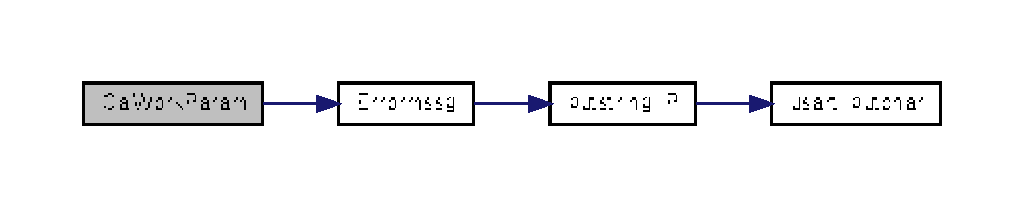
\includegraphics[width=350pt]{group__biba__drv_ga3389079a7106f1e741c0bc447dfbcbca_cgraph}
\end{center}
\end{figure}




Here is the caller graph for this function\-:
\nopagebreak
\begin{figure}[H]
\begin{center}
\leavevmode
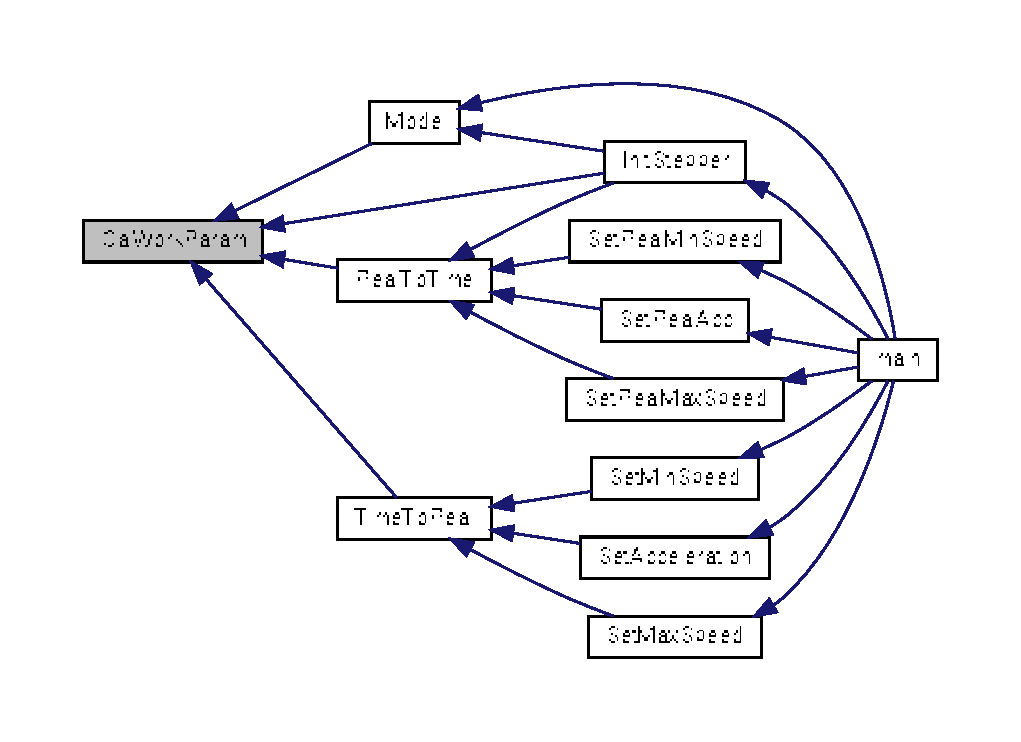
\includegraphics[width=350pt]{group__biba__drv_ga3389079a7106f1e741c0bc447dfbcbca_icgraph}
\end{center}
\end{figure}


\hypertarget{group__biba__drv_ga961e1c89176d3c56101bb4eddf6642dc}{\index{D\-R\-V8825 Library@{D\-R\-V8825 Library}!Count\-\_\-\-Step@{Count\-\_\-\-Step}}
\index{Count\-\_\-\-Step@{Count\-\_\-\-Step}!DRV8825 Library@{D\-R\-V8825 Library}}
\subsubsection[{Count\-\_\-\-Step}]{\setlength{\rightskip}{0pt plus 5cm}void Count\-\_\-\-Step (
\begin{DoxyParamCaption}
\item[{{\bf step\-\_\-type}}]{step, }
\item[{uint64\-\_\-t}]{step\-\_\-count}
\end{DoxyParamCaption}
)}}\label{group__biba__drv_ga961e1c89176d3c56101bb4eddf6642dc}
Initializes the presented steps and calculates the steps for acceleration, deacceleration and the steps for constant speed \begin{DoxySeeAlso}{See Also}
\hyperlink{group__biba__drv_ga3af682b92aa259509aea217f6dc64356}{step\-\_\-type} 
\end{DoxySeeAlso}

\begin{DoxyParams}{Parameters}
{\em step} & the first argument. \\
\hline
{\em step\-\_\-count} & the second argument. \\
\hline
\end{DoxyParams}
\begin{DoxyReturn}{Returns}
void 
\end{DoxyReturn}


Definition at line 297 of file drv\-\_\-8825.\-c.


\begin{DoxyCode}
298 \{
299 
300     uint16\_t y;
301     \hyperlink{drv__8825_8c_a237abe7878c99e9fb1c077c0b916733f}{StepDir} = step;
302 
303 
304     y = ( \hyperlink{drv__8825_8c_a4c86b1f568d93b1bfc8c30587b2c271a}{WorkingParam}.\hyperlink{structMotor__Parameters_aaf0ac3ed818f5c89cc86ea1d9174dc43}{MinSpeed} - \hyperlink{drv__8825_8c_a4c86b1f568d93b1bfc8c30587b2c271a}{WorkingParam}.
      \hyperlink{structMotor__Parameters_a501458e333945f49f03c295e2f49e3b9}{MaxSpeed} ) / \hyperlink{drv__8825_8c_a4c86b1f568d93b1bfc8c30587b2c271a}{WorkingParam}.\hyperlink{structMotor__Parameters_aa9f1146edc6d945d535eec80a01481f1}{Acceleration};
305     y = y << 1;
306     if ( y < step\_count )
307     \{
308         \hyperlink{structMotion}{Motion}.\hyperlink{structMotion_a970d0810aac5cab75c8dd0c95e4473da}{StepsAccel} = y >> 1;
309         \hyperlink{structMotion}{Motion}.\hyperlink{structMotion_a0d7942de8bba5304852a9f2d8fe833e5}{StepsDeaccel} = \hyperlink{structMotion}{Motion}.\hyperlink{structMotion_a970d0810aac5cab75c8dd0c95e4473da}{StepsAccel};
310         \hyperlink{structMotion}{Motion}.\hyperlink{structMotion_aa99fa8cb04ab25fc08e7b65664b7fdef}{StepsConstSpeed} = step\_count - ( \hyperlink{structMotion}{Motion}.
      \hyperlink{structMotion_a970d0810aac5cab75c8dd0c95e4473da}{StepsAccel} + \hyperlink{structMotion}{Motion}.\hyperlink{structMotion_a0d7942de8bba5304852a9f2d8fe833e5}{StepsDeaccel} );
311 
312     \} \textcolor{keywordflow}{else}
313     \{
314         \hyperlink{structMotion}{Motion}.\hyperlink{structMotion_aa99fa8cb04ab25fc08e7b65664b7fdef}{StepsConstSpeed} = 0;
315         \hyperlink{structMotion}{Motion}.\hyperlink{structMotion_a970d0810aac5cab75c8dd0c95e4473da}{StepsAccel} = step\_count >> 1;
316         \hyperlink{structMotion}{Motion}.\hyperlink{structMotion_a0d7942de8bba5304852a9f2d8fe833e5}{StepsDeaccel} = \hyperlink{structMotion}{Motion}.\hyperlink{structMotion_a970d0810aac5cab75c8dd0c95e4473da}{StepsAccel};
317         \textcolor{keywordflow}{if} ( ( step\_count & 1 ) )
318         \{
319             \hyperlink{structMotion}{Motion}.\hyperlink{structMotion_a970d0810aac5cab75c8dd0c95e4473da}{StepsAccel}++;
320         \}
321 
322     \}
323     \hyperlink{group__biba__config_gaf2f231c38a29a96bac24f174fe7bf8b0}{clr\_bit}( TCCR1B, CS10 );
324     \hyperlink{group__biba__config_ga4ee07d04aa2ef10d631d61c17c558464}{set\_bit}( TCCR1B, CS11 );
325     \hyperlink{group__biba__config_gaf2f231c38a29a96bac24f174fe7bf8b0}{clr\_bit}( TCCR1B, CS12 );
326     TCNT1 = 65535 - \hyperlink{drv__8825_8c_a4c86b1f568d93b1bfc8c30587b2c271a}{WorkingParam}.\hyperlink{structMotor__Parameters_aaf0ac3ed818f5c89cc86ea1d9174dc43}{MinSpeed};
327     \hyperlink{structMotion}{Motion}.\hyperlink{structMotion_a50860ebd661de5d104a36a92cd5f17c7}{CurrentSpeed} = \hyperlink{drv__8825_8c_a4c86b1f568d93b1bfc8c30587b2c271a}{WorkingParam}.\hyperlink{structMotor__Parameters_aaf0ac3ed818f5c89cc86ea1d9174dc43}{MinSpeed};
328     \hyperlink{group__biba__config_ga4ee07d04aa2ef10d631d61c17c558464}{set\_bit}( TIMSK, TOIE1 );
329 
330 \}
\end{DoxyCode}


Here is the caller graph for this function\-:
\nopagebreak
\begin{figure}[H]
\begin{center}
\leavevmode
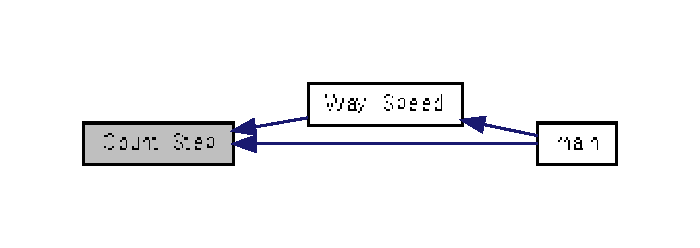
\includegraphics[width=336pt]{group__biba__drv_ga961e1c89176d3c56101bb4eddf6642dc_icgraph}
\end{center}
\end{figure}


\hypertarget{group__biba__drv_gade0e100f335652e364c58ae4a5c89ba4}{\index{D\-R\-V8825 Library@{D\-R\-V8825 Library}!Decay@{Decay}}
\index{Decay@{Decay}!DRV8825 Library@{D\-R\-V8825 Library}}
\subsubsection[{Decay}]{\setlength{\rightskip}{0pt plus 5cm}void Decay (
\begin{DoxyParamCaption}
\item[{{\bf decay\-\_\-type}}]{decay}
\end{DoxyParamCaption}
)}}\label{group__biba__drv_gade0e100f335652e364c58ae4a5c89ba4}
Function that sets the decay type. \begin{DoxySeeAlso}{See Also}
\hyperlink{group__biba__drv_gafe05744bd777532cf059c0d7293a7ab8}{decay\-\_\-type} 
\end{DoxySeeAlso}

\begin{DoxyParams}{Parameters}
{\em decay} & the first argument. \\
\hline
\end{DoxyParams}
\begin{DoxyReturn}{Returns}
void 
\end{DoxyReturn}


Definition at line 185 of file drv\-\_\-8825.\-c.


\begin{DoxyCode}
186 \{
187     \hyperlink{drv__8825_8c_a1cc7e950196402ba79f3e5098b08fa33}{CurrentDecay} = decay;
188     \hyperlink{group__biba__drv_gaaefaac2ed4c54f2008d8d236392c7261}{store}( );
189     \textcolor{keywordflow}{if} ( decay == \hyperlink{group__biba__drv_ggafe05744bd777532cf059c0d7293a7ab8af9716e06b54f75cbd7dedc154a7d49e2}{FAST\_DECAY} )
190     \{
191         \hyperlink{group__biba__config_ga91fb0adcf6533b4acfe793396836badc}{set\_as\_output}( \hyperlink{group__biba__config_ga4280725e4eff1145eac3e34c574b8383}{DDECAY}, \hyperlink{group__biba__config_ga9d211c41bcae2aa62028a3645c63cf8a}{DECAY} );
192         \hyperlink{group__biba__config_ga4ee07d04aa2ef10d631d61c17c558464}{set\_bit}( \hyperlink{group__biba__config_ga42a58bd5ca7d52e02b78dbc498bd18fc}{PDECAY}, \hyperlink{group__biba__config_ga9d211c41bcae2aa62028a3645c63cf8a}{DECAY} );
193         \textcolor{keywordflow}{return};
194     \}
195 
196     \textcolor{keywordflow}{if} ( decay == \hyperlink{group__biba__drv_ggafe05744bd777532cf059c0d7293a7ab8a05f6a902065ce2f3355101cf657f4ba4}{SLOW\_DECAY} )
197     \{
198         \hyperlink{group__biba__config_ga91fb0adcf6533b4acfe793396836badc}{set\_as\_output}( \hyperlink{group__biba__config_ga4280725e4eff1145eac3e34c574b8383}{DDECAY}, \hyperlink{group__biba__config_ga9d211c41bcae2aa62028a3645c63cf8a}{DECAY} );
199         \hyperlink{group__biba__config_gaf2f231c38a29a96bac24f174fe7bf8b0}{clr\_bit}( \hyperlink{group__biba__config_ga42a58bd5ca7d52e02b78dbc498bd18fc}{PDECAY}, \hyperlink{group__biba__config_ga9d211c41bcae2aa62028a3645c63cf8a}{DECAY} );
200         \textcolor{keywordflow}{return};
201     \}
202 
203     \hyperlink{group__biba__config_gaf5147cefc7b56baad8c6337a315ce07f}{set\_as\_input}( \hyperlink{group__biba__config_ga4280725e4eff1145eac3e34c574b8383}{DDECAY}, \hyperlink{group__biba__config_ga9d211c41bcae2aa62028a3645c63cf8a}{DECAY} );
204     \hyperlink{group__biba__config_gaf2f231c38a29a96bac24f174fe7bf8b0}{clr\_bit}( \hyperlink{group__biba__config_ga42a58bd5ca7d52e02b78dbc498bd18fc}{PDECAY}, \hyperlink{group__biba__config_ga9d211c41bcae2aa62028a3645c63cf8a}{DECAY} );
205 \}
\end{DoxyCode}


Here is the call graph for this function\-:
\nopagebreak
\begin{figure}[H]
\begin{center}
\leavevmode
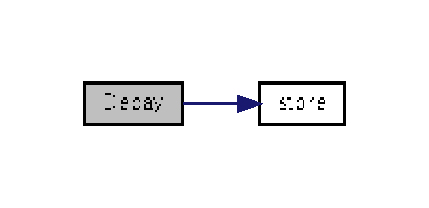
\includegraphics[width=206pt]{group__biba__drv_gade0e100f335652e364c58ae4a5c89ba4_cgraph}
\end{center}
\end{figure}




Here is the caller graph for this function\-:
\nopagebreak
\begin{figure}[H]
\begin{center}
\leavevmode
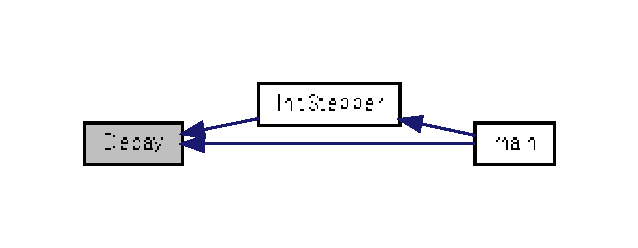
\includegraphics[width=306pt]{group__biba__drv_gade0e100f335652e364c58ae4a5c89ba4_icgraph}
\end{center}
\end{figure}


\hypertarget{group__biba__drv_ga5b763d9479149e1cd8843fa5f144a18a}{\index{D\-R\-V8825 Library@{D\-R\-V8825 Library}!Disabled\-\_\-\-Stepper@{Disabled\-\_\-\-Stepper}}
\index{Disabled\-\_\-\-Stepper@{Disabled\-\_\-\-Stepper}!DRV8825 Library@{D\-R\-V8825 Library}}
\subsubsection[{Disabled\-\_\-\-Stepper}]{\setlength{\rightskip}{0pt plus 5cm}void Disabled\-\_\-\-Stepper (
\begin{DoxyParamCaption}
\item[{void}]{}
\end{DoxyParamCaption}
)}}\label{group__biba__drv_ga5b763d9479149e1cd8843fa5f144a18a}
Function that disables the stepper motor. \begin{DoxyReturn}{Returns}
void 
\end{DoxyReturn}


Definition at line 173 of file drv\-\_\-8825.\-c.


\begin{DoxyCode}
174 \{
175     \hyperlink{group__biba__config_ga4ee07d04aa2ef10d631d61c17c558464}{set\_bit}( \hyperlink{group__biba__config_gaf49566bede8af55a9c7c7cb49722ca8a}{PENABLE\_STEPPER}, \hyperlink{group__biba__config_gaf43f2237d47f7e2e48d74999befaa9fd}{ENABLE\_STEPPER} );
176     \hyperlink{drv__8825_8c_ac23af1c3ab9ed8b840ff803e637bf070}{ModeStart} = 0;
177 \}
\end{DoxyCode}


Here is the caller graph for this function\-:
\nopagebreak
\begin{figure}[H]
\begin{center}
\leavevmode
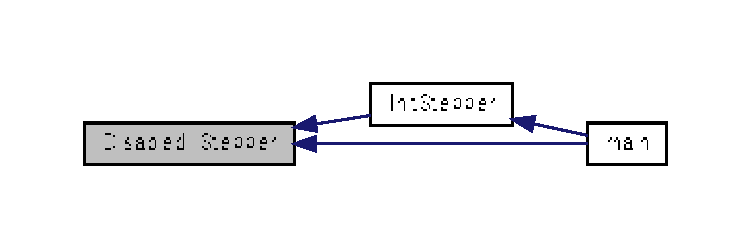
\includegraphics[width=350pt]{group__biba__drv_ga5b763d9479149e1cd8843fa5f144a18a_icgraph}
\end{center}
\end{figure}


\hypertarget{group__biba__drv_gab1ea57d26402b13aaed719a4d11097d5}{\index{D\-R\-V8825 Library@{D\-R\-V8825 Library}!Enable\-\_\-\-Stepper@{Enable\-\_\-\-Stepper}}
\index{Enable\-\_\-\-Stepper@{Enable\-\_\-\-Stepper}!DRV8825 Library@{D\-R\-V8825 Library}}
\subsubsection[{Enable\-\_\-\-Stepper}]{\setlength{\rightskip}{0pt plus 5cm}void Enable\-\_\-\-Stepper (
\begin{DoxyParamCaption}
\item[{void}]{}
\end{DoxyParamCaption}
)}}\label{group__biba__drv_gab1ea57d26402b13aaed719a4d11097d5}
Function that enables the stepper motor. \begin{DoxyReturn}{Returns}
void 
\end{DoxyReturn}


Definition at line 163 of file drv\-\_\-8825.\-c.


\begin{DoxyCode}
164 \{
165     \hyperlink{group__biba__config_gaf2f231c38a29a96bac24f174fe7bf8b0}{clr\_bit}( \hyperlink{group__biba__config_gaf49566bede8af55a9c7c7cb49722ca8a}{PENABLE\_STEPPER}, \hyperlink{group__biba__config_gaf43f2237d47f7e2e48d74999befaa9fd}{ENABLE\_STEPPER} );
166     \hyperlink{drv__8825_8c_ac23af1c3ab9ed8b840ff803e637bf070}{ModeStart} = 1;
167 \}
\end{DoxyCode}


Here is the caller graph for this function\-:
\nopagebreak
\begin{figure}[H]
\begin{center}
\leavevmode
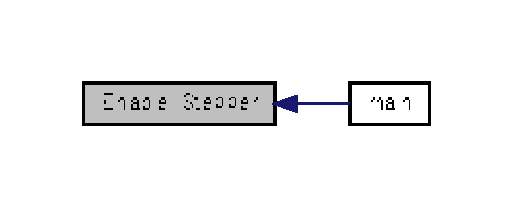
\includegraphics[width=246pt]{group__biba__drv_gab1ea57d26402b13aaed719a4d11097d5_icgraph}
\end{center}
\end{figure}


\hypertarget{group__biba__drv_ga20503ca831d18cf625abe0f6e98d281a}{\index{D\-R\-V8825 Library@{D\-R\-V8825 Library}!Get\-\_\-\-Decay@{Get\-\_\-\-Decay}}
\index{Get\-\_\-\-Decay@{Get\-\_\-\-Decay}!DRV8825 Library@{D\-R\-V8825 Library}}
\subsubsection[{Get\-\_\-\-Decay}]{\setlength{\rightskip}{0pt plus 5cm}{\bf decay\-\_\-type} Get\-\_\-\-Decay (
\begin{DoxyParamCaption}
\item[{void}]{}
\end{DoxyParamCaption}
)}}\label{group__biba__drv_ga20503ca831d18cf625abe0f6e98d281a}
Reads the setted decay. \begin{DoxySeeAlso}{See Also}
\hyperlink{group__biba__drv_gafe05744bd777532cf059c0d7293a7ab8}{decay\-\_\-type} 
\end{DoxySeeAlso}
\begin{DoxyReturn}{Returns}
decay\-\_\-type 
\end{DoxyReturn}


Definition at line 395 of file drv\-\_\-8825.\-c.


\begin{DoxyCode}
396 \{
397     \textcolor{keywordflow}{return} \hyperlink{drv__8825_8c_a1cc7e950196402ba79f3e5098b08fa33}{CurrentDecay};
398 \}
\end{DoxyCode}


Here is the caller graph for this function\-:
\nopagebreak
\begin{figure}[H]
\begin{center}
\leavevmode
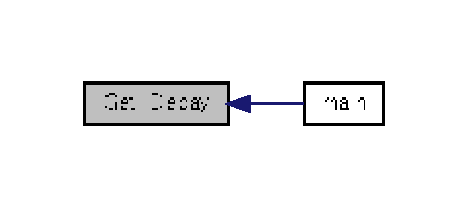
\includegraphics[width=224pt]{group__biba__drv_ga20503ca831d18cf625abe0f6e98d281a_icgraph}
\end{center}
\end{figure}


\hypertarget{group__biba__drv_ga51c375fddbfeaed5366cd0bf2f9a2dab}{\index{D\-R\-V8825 Library@{D\-R\-V8825 Library}!Get\-\_\-\-Mode@{Get\-\_\-\-Mode}}
\index{Get\-\_\-\-Mode@{Get\-\_\-\-Mode}!DRV8825 Library@{D\-R\-V8825 Library}}
\subsubsection[{Get\-\_\-\-Mode}]{\setlength{\rightskip}{0pt plus 5cm}{\bf mode\-\_\-type} Get\-\_\-\-Mode (
\begin{DoxyParamCaption}
\item[{void}]{}
\end{DoxyParamCaption}
)}}\label{group__biba__drv_ga51c375fddbfeaed5366cd0bf2f9a2dab}
Reads the setted mode. \begin{DoxySeeAlso}{See Also}
\hyperlink{group__biba__drv_ga19269c193c0c4866cdc4e5abd433f9fc}{mode\-\_\-type} 
\end{DoxySeeAlso}
\begin{DoxyReturn}{Returns}
mode\-\_\-type 
\end{DoxyReturn}


Definition at line 405 of file drv\-\_\-8825.\-c.


\begin{DoxyCode}
406 \{
407     \textcolor{keywordflow}{return} \hyperlink{drv__8825_8c_ab08e51d202664c8cc9434eac6c46f1f3}{CurrentMode};
408 \}
\end{DoxyCode}


Here is the caller graph for this function\-:
\nopagebreak
\begin{figure}[H]
\begin{center}
\leavevmode
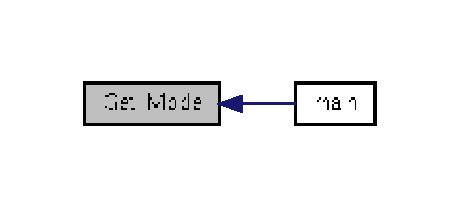
\includegraphics[width=220pt]{group__biba__drv_ga51c375fddbfeaed5366cd0bf2f9a2dab_icgraph}
\end{center}
\end{figure}


\hypertarget{group__biba__drv_gabdfa1389f4c68fca40077275f7727fea}{\index{D\-R\-V8825 Library@{D\-R\-V8825 Library}!Get\-\_\-\-Start@{Get\-\_\-\-Start}}
\index{Get\-\_\-\-Start@{Get\-\_\-\-Start}!DRV8825 Library@{D\-R\-V8825 Library}}
\subsubsection[{Get\-\_\-\-Start}]{\setlength{\rightskip}{0pt plus 5cm}uint8\-\_\-t Get\-\_\-\-Start (
\begin{DoxyParamCaption}
\item[{void}]{}
\end{DoxyParamCaption}
)}}\label{group__biba__drv_gabdfa1389f4c68fca40077275f7727fea}
Returns the mode. \begin{DoxyReturn}{Returns}
uint8\-\_\-t 
\end{DoxyReturn}


Definition at line 414 of file drv\-\_\-8825.\-c.


\begin{DoxyCode}
415 \{
416     \textcolor{keywordflow}{return} \hyperlink{drv__8825_8c_ac23af1c3ab9ed8b840ff803e637bf070}{ModeStart};
417 \}
\end{DoxyCode}


Here is the caller graph for this function\-:
\nopagebreak
\begin{figure}[H]
\begin{center}
\leavevmode
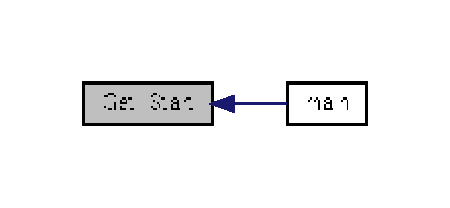
\includegraphics[width=216pt]{group__biba__drv_gabdfa1389f4c68fca40077275f7727fea_icgraph}
\end{center}
\end{figure}


\hypertarget{group__biba__drv_ga5591760e7dd32c026ec449f0d516af28}{\index{D\-R\-V8825 Library@{D\-R\-V8825 Library}!Get\-\_\-\-Steps\-\_\-revol@{Get\-\_\-\-Steps\-\_\-revol}}
\index{Get\-\_\-\-Steps\-\_\-revol@{Get\-\_\-\-Steps\-\_\-revol}!DRV8825 Library@{D\-R\-V8825 Library}}
\subsubsection[{Get\-\_\-\-Steps\-\_\-revol}]{\setlength{\rightskip}{0pt plus 5cm}uint16\-\_\-t Get\-\_\-\-Steps\-\_\-revol (
\begin{DoxyParamCaption}
\item[{void}]{}
\end{DoxyParamCaption}
)}}\label{group__biba__drv_ga5591760e7dd32c026ec449f0d516af28}
Gets the steps per revolution. \begin{DoxySeeAlso}{See Also}
\hyperlink{drv__8825_8c_a54128bfe0cfae9cbd8577cf456951f21}{Steps\-Per\-Rev} 
\end{DoxySeeAlso}
\begin{DoxyReturn}{Returns}
uint16\-\_\-t 
\end{DoxyReturn}


Definition at line 545 of file drv\-\_\-8825.\-c.


\begin{DoxyCode}
546 \{
547     \textcolor{keywordflow}{return} \hyperlink{drv__8825_8c_a54128bfe0cfae9cbd8577cf456951f21}{StepsPerRev};
548 \}
\end{DoxyCode}


Here is the caller graph for this function\-:
\nopagebreak
\begin{figure}[H]
\begin{center}
\leavevmode
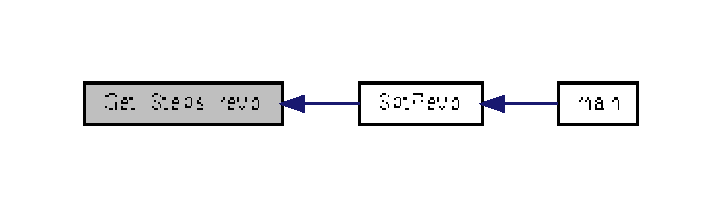
\includegraphics[width=346pt]{group__biba__drv_ga5591760e7dd32c026ec449f0d516af28_icgraph}
\end{center}
\end{figure}


\hypertarget{group__biba__drv_ga6202c4fd41a45376809e5940428467b9}{\index{D\-R\-V8825 Library@{D\-R\-V8825 Library}!Get\-Acceleration@{Get\-Acceleration}}
\index{Get\-Acceleration@{Get\-Acceleration}!DRV8825 Library@{D\-R\-V8825 Library}}
\subsubsection[{Get\-Acceleration}]{\setlength{\rightskip}{0pt plus 5cm}uint16\-\_\-t Get\-Acceleration (
\begin{DoxyParamCaption}
\item[{void}]{}
\end{DoxyParamCaption}
)}}\label{group__biba__drv_ga6202c4fd41a45376809e5940428467b9}
Reads the setted acceleration. \begin{DoxySeeAlso}{See Also}
Time\-Param.\-Acceleration 
\end{DoxySeeAlso}
\begin{DoxyReturn}{Returns}
uint16\-\_\-t 
\end{DoxyReturn}


Definition at line 445 of file drv\-\_\-8825.\-c.


\begin{DoxyCode}
446 \{
447     \textcolor{keywordflow}{return} \hyperlink{drv__8825_8c_a7d20b8cec6f96108790d4bf76b9c469d}{TimeParam}.\hyperlink{structMotor__Parameters_aa9f1146edc6d945d535eec80a01481f1}{Acceleration};
448 \}
\end{DoxyCode}


Here is the caller graph for this function\-:
\nopagebreak
\begin{figure}[H]
\begin{center}
\leavevmode
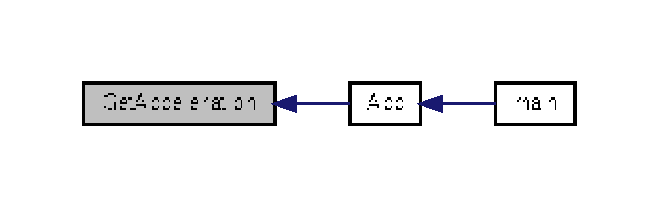
\includegraphics[width=316pt]{group__biba__drv_ga6202c4fd41a45376809e5940428467b9_icgraph}
\end{center}
\end{figure}


\hypertarget{group__biba__drv_ga56c30e2b82a23aed1c9febd704166090}{\index{D\-R\-V8825 Library@{D\-R\-V8825 Library}!Get\-Current\-Speed@{Get\-Current\-Speed}}
\index{Get\-Current\-Speed@{Get\-Current\-Speed}!DRV8825 Library@{D\-R\-V8825 Library}}
\subsubsection[{Get\-Current\-Speed}]{\setlength{\rightskip}{0pt plus 5cm}uint16\-\_\-t Get\-Current\-Speed (
\begin{DoxyParamCaption}
\item[{void}]{}
\end{DoxyParamCaption}
)}}\label{group__biba__drv_ga56c30e2b82a23aed1c9febd704166090}
Reads the current speed. \begin{DoxySeeAlso}{See Also}
Time\-Param.\-Current\-Speed 
\end{DoxySeeAlso}
\begin{DoxyReturn}{Returns}
uint16\-\_\-t 
\end{DoxyReturn}


Definition at line 456 of file drv\-\_\-8825.\-c.


\begin{DoxyCode}
457 \{
458     \textcolor{keywordflow}{return} \hyperlink{structMotion}{Motion}.\hyperlink{structMotion_a50860ebd661de5d104a36a92cd5f17c7}{CurrentSpeed};
459 \}
\end{DoxyCode}
\hypertarget{group__biba__drv_ga356f958c8327643ae22d240493ae7747}{\index{D\-R\-V8825 Library@{D\-R\-V8825 Library}!Get\-Max\-Speed@{Get\-Max\-Speed}}
\index{Get\-Max\-Speed@{Get\-Max\-Speed}!DRV8825 Library@{D\-R\-V8825 Library}}
\subsubsection[{Get\-Max\-Speed}]{\setlength{\rightskip}{0pt plus 5cm}uint16\-\_\-t Get\-Max\-Speed (
\begin{DoxyParamCaption}
\item[{void}]{}
\end{DoxyParamCaption}
)}}\label{group__biba__drv_ga356f958c8327643ae22d240493ae7747}
Reads the setted maximum speed.. \begin{DoxySeeAlso}{See Also}
Time\-Param.\-Max\-Speed 
\end{DoxySeeAlso}
\begin{DoxyReturn}{Returns}
uint16\-\_\-t 
\end{DoxyReturn}


Definition at line 424 of file drv\-\_\-8825.\-c.


\begin{DoxyCode}
425 \{
426     \textcolor{keywordflow}{return} \hyperlink{drv__8825_8c_a7d20b8cec6f96108790d4bf76b9c469d}{TimeParam}.\hyperlink{structMotor__Parameters_a501458e333945f49f03c295e2f49e3b9}{MaxSpeed};
427 \}
\end{DoxyCode}


Here is the caller graph for this function\-:
\nopagebreak
\begin{figure}[H]
\begin{center}
\leavevmode
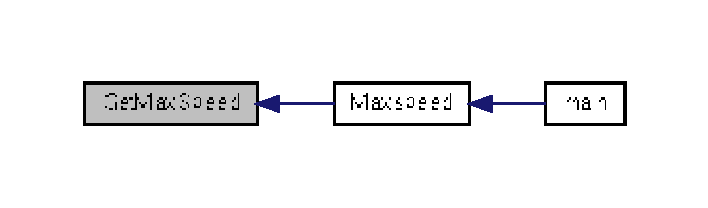
\includegraphics[width=340pt]{group__biba__drv_ga356f958c8327643ae22d240493ae7747_icgraph}
\end{center}
\end{figure}


\hypertarget{group__biba__drv_gab0cfe10ce4af9fb931391f171566fef2}{\index{D\-R\-V8825 Library@{D\-R\-V8825 Library}!Get\-Min\-Speed@{Get\-Min\-Speed}}
\index{Get\-Min\-Speed@{Get\-Min\-Speed}!DRV8825 Library@{D\-R\-V8825 Library}}
\subsubsection[{Get\-Min\-Speed}]{\setlength{\rightskip}{0pt plus 5cm}uint16\-\_\-t Get\-Min\-Speed (
\begin{DoxyParamCaption}
\item[{void}]{}
\end{DoxyParamCaption}
)}}\label{group__biba__drv_gab0cfe10ce4af9fb931391f171566fef2}
Reads the setted minimum speed. \begin{DoxySeeAlso}{See Also}
Time\-Param.\-Min\-Speed 
\end{DoxySeeAlso}
\begin{DoxyReturn}{Returns}
uint16\-\_\-t 
\end{DoxyReturn}


Definition at line 435 of file drv\-\_\-8825.\-c.


\begin{DoxyCode}
436 \{
437     \textcolor{keywordflow}{return} \hyperlink{drv__8825_8c_a7d20b8cec6f96108790d4bf76b9c469d}{TimeParam}.\hyperlink{structMotor__Parameters_aaf0ac3ed818f5c89cc86ea1d9174dc43}{MinSpeed};
438 \}
\end{DoxyCode}


Here is the caller graph for this function\-:
\nopagebreak
\begin{figure}[H]
\begin{center}
\leavevmode
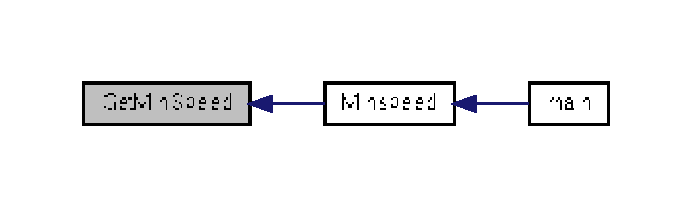
\includegraphics[width=332pt]{group__biba__drv_gab0cfe10ce4af9fb931391f171566fef2_icgraph}
\end{center}
\end{figure}


\hypertarget{group__biba__drv_ga819f85ff37467b16c6e6e31ffc858619}{\index{D\-R\-V8825 Library@{D\-R\-V8825 Library}!Get\-Real\-Acc@{Get\-Real\-Acc}}
\index{Get\-Real\-Acc@{Get\-Real\-Acc}!DRV8825 Library@{D\-R\-V8825 Library}}
\subsubsection[{Get\-Real\-Acc}]{\setlength{\rightskip}{0pt plus 5cm}uint16\-\_\-t Get\-Real\-Acc (
\begin{DoxyParamCaption}
\item[{void}]{}
\end{DoxyParamCaption}
)}}\label{group__biba__drv_ga819f85ff37467b16c6e6e31ffc858619}
Gets the real acceleration. \begin{DoxySeeAlso}{See Also}
Real\-Speed.\-Acceleration 
\end{DoxySeeAlso}
\begin{DoxyReturn}{Returns}
uint16\-\_\-t 
\end{DoxyReturn}


Definition at line 613 of file drv\-\_\-8825.\-c.


\begin{DoxyCode}
614 \{
615     \textcolor{keywordflow}{return} \hyperlink{drv__8825_8c_a2e720ed1ed0ef90dba27c1f246048dcd}{RealSpeed}.\hyperlink{structMotor__Parameters_aa9f1146edc6d945d535eec80a01481f1}{Acceleration};
616 \}
\end{DoxyCode}


Here is the caller graph for this function\-:
\nopagebreak
\begin{figure}[H]
\begin{center}
\leavevmode
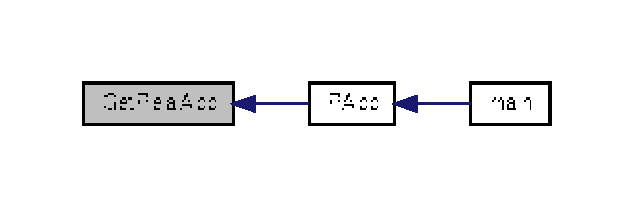
\includegraphics[width=304pt]{group__biba__drv_ga819f85ff37467b16c6e6e31ffc858619_icgraph}
\end{center}
\end{figure}


\hypertarget{group__biba__drv_ga20bfcaca6af265d5f8b2dc50f3a26779}{\index{D\-R\-V8825 Library@{D\-R\-V8825 Library}!Get\-Real\-Max\-Speed@{Get\-Real\-Max\-Speed}}
\index{Get\-Real\-Max\-Speed@{Get\-Real\-Max\-Speed}!DRV8825 Library@{D\-R\-V8825 Library}}
\subsubsection[{Get\-Real\-Max\-Speed}]{\setlength{\rightskip}{0pt plus 5cm}uint16\-\_\-t Get\-Real\-Max\-Speed (
\begin{DoxyParamCaption}
\item[{void}]{}
\end{DoxyParamCaption}
)}}\label{group__biba__drv_ga20bfcaca6af265d5f8b2dc50f3a26779}
Gets the real maximum speed. \begin{DoxySeeAlso}{See Also}
Real\-Speed.\-Max\-Speed 
\end{DoxySeeAlso}
\begin{DoxyReturn}{Returns}
uint16\-\_\-t 
\end{DoxyReturn}


Definition at line 592 of file drv\-\_\-8825.\-c.


\begin{DoxyCode}
593 \{
594     \textcolor{keywordflow}{return} \hyperlink{drv__8825_8c_a2e720ed1ed0ef90dba27c1f246048dcd}{RealSpeed}.\hyperlink{structMotor__Parameters_a501458e333945f49f03c295e2f49e3b9}{MaxSpeed};
595 \}
\end{DoxyCode}


Here is the caller graph for this function\-:
\nopagebreak
\begin{figure}[H]
\begin{center}
\leavevmode
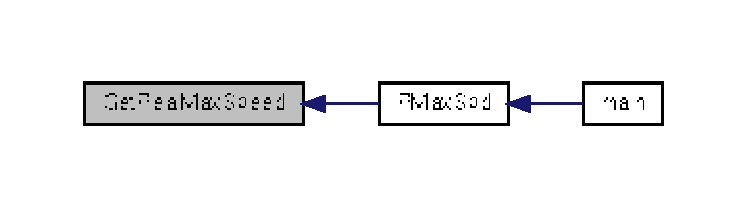
\includegraphics[width=350pt]{group__biba__drv_ga20bfcaca6af265d5f8b2dc50f3a26779_icgraph}
\end{center}
\end{figure}


\hypertarget{group__biba__drv_ga6fdcb3b4ad128890ee607c75a92e63a8}{\index{D\-R\-V8825 Library@{D\-R\-V8825 Library}!Get\-Real\-Min\-Speed@{Get\-Real\-Min\-Speed}}
\index{Get\-Real\-Min\-Speed@{Get\-Real\-Min\-Speed}!DRV8825 Library@{D\-R\-V8825 Library}}
\subsubsection[{Get\-Real\-Min\-Speed}]{\setlength{\rightskip}{0pt plus 5cm}uint16\-\_\-t Get\-Real\-Min\-Speed (
\begin{DoxyParamCaption}
\item[{void}]{}
\end{DoxyParamCaption}
)}}\label{group__biba__drv_ga6fdcb3b4ad128890ee607c75a92e63a8}
Gets the real minimum speed. \begin{DoxySeeAlso}{See Also}
Real\-Speed.\-Min\-Speed 
\end{DoxySeeAlso}
\begin{DoxyReturn}{Returns}
uint16\-\_\-t 
\end{DoxyReturn}


Definition at line 603 of file drv\-\_\-8825.\-c.


\begin{DoxyCode}
604 \{
605     \textcolor{keywordflow}{return} \hyperlink{drv__8825_8c_a2e720ed1ed0ef90dba27c1f246048dcd}{RealSpeed}.\hyperlink{structMotor__Parameters_aaf0ac3ed818f5c89cc86ea1d9174dc43}{MinSpeed};
606 \}
\end{DoxyCode}


Here is the caller graph for this function\-:
\nopagebreak
\begin{figure}[H]
\begin{center}
\leavevmode
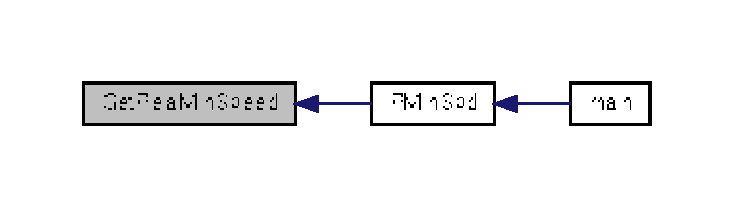
\includegraphics[width=350pt]{group__biba__drv_ga6fdcb3b4ad128890ee607c75a92e63a8_icgraph}
\end{center}
\end{figure}


\hypertarget{group__biba__drv_ga8f3808b2e4aa3b2a8f6467a2aaa31995}{\index{D\-R\-V8825 Library@{D\-R\-V8825 Library}!Helper\-Rto\-T@{Helper\-Rto\-T}}
\index{Helper\-Rto\-T@{Helper\-Rto\-T}!DRV8825 Library@{D\-R\-V8825 Library}}
\subsubsection[{Helper\-Rto\-T}]{\setlength{\rightskip}{0pt plus 5cm}uint64\-\_\-t Helper\-Rto\-T (
\begin{DoxyParamCaption}
\item[{uint64\-\_\-t}]{in}
\end{DoxyParamCaption}
)}}\label{group__biba__drv_ga8f3808b2e4aa3b2a8f6467a2aaa31995}
Helper of the function Real\-To\-Time \begin{DoxySeeAlso}{See Also}
\hyperlink{group__biba__drv_gad23127bea36c997c0b1c767f2421db6a}{Real\-To\-Time} 
\end{DoxySeeAlso}

\begin{DoxyParams}{Parameters}
{\em in} & the first argument. \\
\hline
\end{DoxyParams}
\begin{DoxyReturn}{Returns}
uint64\-\_\-t 
\end{DoxyReturn}


Definition at line 838 of file drv\-\_\-8825.\-c.


\begin{DoxyCode}
839 \{
840     uint64\_t revpermin;
841 
842 \textcolor{comment}{/*}
843 \textcolor{comment}{    revpermin = in;}
844 \textcolor{comment}{    revpermin = revpermin*StepsPerRev;}
845 \textcolor{comment}{    revpermin = revpermin / 60;}
846 \textcolor{comment}{    revpermin = 1000000000 / revpermin;}
847 \textcolor{comment}{    revpermin = revpermin / PERTMR;}
848 \textcolor{comment}{*/}
849 revpermin=\hyperlink{drv__8825_8c_a556953635433b080667d6e8888dfe876}{TIMERCONST}/(in*\hyperlink{drv__8825_8c_a54128bfe0cfae9cbd8577cf456951f21}{StepsPerRev});
850     \textcolor{keywordflow}{if} ( revpermin < 65500 )
851     \{   
852         \textcolor{keywordflow}{return} revpermin;
853     \}
854     \textcolor{keywordflow}{else}
855     \{
856         \textcolor{keywordflow}{return}  65500;
857     \}
858 \}
\end{DoxyCode}


Here is the caller graph for this function\-:
\nopagebreak
\begin{figure}[H]
\begin{center}
\leavevmode
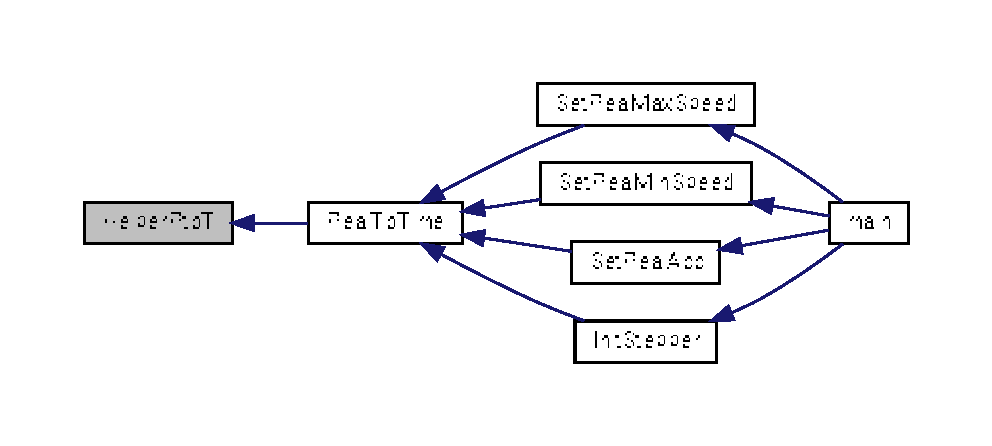
\includegraphics[width=350pt]{group__biba__drv_ga8f3808b2e4aa3b2a8f6467a2aaa31995_icgraph}
\end{center}
\end{figure}


\hypertarget{group__biba__drv_gabc1e78364b977fdff7ae3b642e720f58}{\index{D\-R\-V8825 Library@{D\-R\-V8825 Library}!Helper\-Tto\-R@{Helper\-Tto\-R}}
\index{Helper\-Tto\-R@{Helper\-Tto\-R}!DRV8825 Library@{D\-R\-V8825 Library}}
\subsubsection[{Helper\-Tto\-R}]{\setlength{\rightskip}{0pt plus 5cm}uint64\-\_\-t Helper\-Tto\-R (
\begin{DoxyParamCaption}
\item[{uint64\-\_\-t}]{in}
\end{DoxyParamCaption}
)}}\label{group__biba__drv_gabc1e78364b977fdff7ae3b642e720f58}
Helper of the function Time\-To\-Real \begin{DoxySeeAlso}{See Also}
\hyperlink{group__biba__drv_gaec239a01fef85140bc7c12fa612f421b}{Time\-To\-Real} 
\end{DoxySeeAlso}

\begin{DoxyParams}{Parameters}
{\em in} & the first argument. \\
\hline
\end{DoxyParams}
\begin{DoxyReturn}{Returns}
uint64\-\_\-t 
\end{DoxyReturn}


Definition at line 867 of file drv\-\_\-8825.\-c.


\begin{DoxyCode}
868 \{
869     uint64\_t r;
870 
871     \textcolor{comment}{//const uint64\_t l=1000000000*60;}
872     
873     r=\hyperlink{drv__8825_8c_a556953635433b080667d6e8888dfe876}{TIMERCONST}/(in*\hyperlink{drv__8825_8c_a54128bfe0cfae9cbd8577cf456951f21}{StepsPerRev});
874     
875 \textcolor{comment}{/*}
876 \textcolor{comment}{    r = in;}
877 \textcolor{comment}{}
878 \textcolor{comment}{    }
879 \textcolor{comment}{    }
880 \textcolor{comment}{    r = r * PERTMR;}
881 \textcolor{comment}{    r = r*StepsPerRev;}
882 \textcolor{comment}{    r = 10000000000 / r;}
883 \textcolor{comment}{    r = r * 6;}
884 \textcolor{comment}{}
885 \textcolor{comment}{*/}
886 
887 
888 
889     \textcolor{keywordflow}{if} ( r > 1 )
890     \{
891         \textcolor{keywordflow}{return} r;
892     \} \textcolor{keywordflow}{else}
893     \{
894         \textcolor{keywordflow}{return} 1;
895         \textcolor{comment}{//putstring\_P( PSTR( "Target MaxSpeed\(\backslash\)r" ) );}
896     \}
897 
898 \}
\end{DoxyCode}


Here is the caller graph for this function\-:
\nopagebreak
\begin{figure}[H]
\begin{center}
\leavevmode
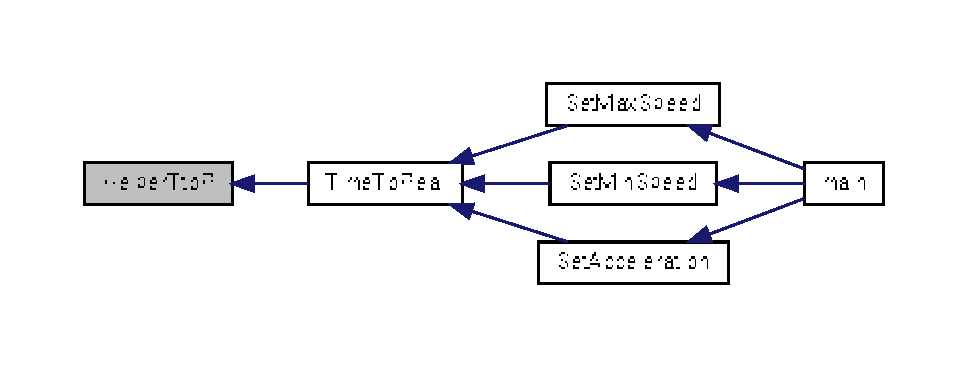
\includegraphics[width=350pt]{group__biba__drv_gabc1e78364b977fdff7ae3b642e720f58_icgraph}
\end{center}
\end{figure}


\hypertarget{group__biba__drv_gaf24afdf808aa610fe7471985b03ea134}{\index{D\-R\-V8825 Library@{D\-R\-V8825 Library}!Home@{Home}}
\index{Home@{Home}!DRV8825 Library@{D\-R\-V8825 Library}}
\subsubsection[{Home}]{\setlength{\rightskip}{0pt plus 5cm}uint8\-\_\-t Home (
\begin{DoxyParamCaption}
\item[{void}]{}
\end{DoxyParamCaption}
)}}\label{group__biba__drv_gaf24afdf808aa610fe7471985b03ea134}
The home of the motor. \begin{DoxyRefDesc}{Todo}
\item[\hyperlink{todo__todo000001}{Todo}]it doesnt work as espected \end{DoxyRefDesc}
\begin{DoxySeeAlso}{See Also}
\hyperlink{group__biba__drv_ga3af682b92aa259509aea217f6dc64356}{step\-\_\-type} 
\end{DoxySeeAlso}
\begin{DoxyReturn}{Returns}
uint8\-\_\-t 
\end{DoxyReturn}


Definition at line 376 of file drv\-\_\-8825.\-c.


\begin{DoxyCode}
377 \{
378     int16\_t i;
379 
380     \textcolor{keywordflow}{for} ( i = 0; i < 128; i++ )
381     \{
382         \hyperlink{group__biba__drv_ga7920069eba0a349a19a7e5af32321ad8}{Step}(\hyperlink{group__biba__drv_gga3af682b92aa259509aea217f6dc64356a05e804aea3cc6dd53f5d5a836d0365c9}{STEP\_COUNTER\_CLOCKWISE});
383         \textcolor{keywordflow}{if} ( !(\hyperlink{group__biba__config_ga65a9fed63ff97399d2b08295253076f3}{check\_pin}( \hyperlink{group__biba__config_gabd13263a1daa3de2c2e1417449c8e476}{IHOME}, \hyperlink{group__biba__config_ga0e26ea2db1b570d1a6fe1ac180ef4541}{HOME} )) )
384             \textcolor{keywordflow}{return} \textcolor{keyword}{true};
385     \}
386     \textcolor{keywordflow}{return} \textcolor{keyword}{false};
387 \}
\end{DoxyCode}


Here is the call graph for this function\-:
\nopagebreak
\begin{figure}[H]
\begin{center}
\leavevmode
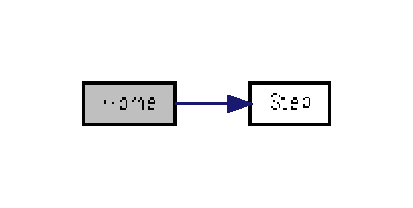
\includegraphics[width=198pt]{group__biba__drv_gaf24afdf808aa610fe7471985b03ea134_cgraph}
\end{center}
\end{figure}


\hypertarget{group__biba__drv_gad7c735bb7a3e49bba5cb72962f045d10}{\index{D\-R\-V8825 Library@{D\-R\-V8825 Library}!Init\-Stepper@{Init\-Stepper}}
\index{Init\-Stepper@{Init\-Stepper}!DRV8825 Library@{D\-R\-V8825 Library}}
\subsubsection[{Init\-Stepper}]{\setlength{\rightskip}{0pt plus 5cm}void Init\-Stepper (
\begin{DoxyParamCaption}
\item[{void}]{}
\end{DoxyParamCaption}
)}}\label{group__biba__drv_gad7c735bb7a3e49bba5cb72962f045d10}
Initialize the D\-R\-V232. \begin{DoxyReturn}{Returns}
void 
\end{DoxyReturn}


Definition at line 778 of file drv\-\_\-8825.\-c.


\begin{DoxyCode}
779 \{
780     \hyperlink{drv__8825_8c_a2e720ed1ed0ef90dba27c1f246048dcd}{RealSpeed}.\hyperlink{structMotor__Parameters_a501458e333945f49f03c295e2f49e3b9}{MaxSpeed} = eeprom\_read\_word( ( uint16\_t * ) ( 0 ) );
781     \hyperlink{drv__8825_8c_a2e720ed1ed0ef90dba27c1f246048dcd}{RealSpeed}.\hyperlink{structMotor__Parameters_aaf0ac3ed818f5c89cc86ea1d9174dc43}{MinSpeed} = eeprom\_read\_word( ( uint16\_t * ) ( 2 ) );
782     \hyperlink{drv__8825_8c_a2e720ed1ed0ef90dba27c1f246048dcd}{RealSpeed}.\hyperlink{structMotor__Parameters_aa9f1146edc6d945d535eec80a01481f1}{Acceleration} = eeprom\_read\_word( ( uint16\_t * ) ( 4 ) );
783     \hyperlink{drv__8825_8c_a54128bfe0cfae9cbd8577cf456951f21}{StepsPerRev} = eeprom\_read\_word( ( uint16\_t * ) ( 6 ) );
784     \hyperlink{drv__8825_8c_ab08e51d202664c8cc9434eac6c46f1f3}{CurrentMode} = eeprom\_read\_byte( ( uint8\_t * ) ( 8 ) );
785     \hyperlink{drv__8825_8c_a1cc7e950196402ba79f3e5098b08fa33}{CurrentDecay} = eeprom\_read\_byte( ( uint8\_t * ) ( 9 ) );
786     \textcolor{keywordflow}{if} ( ( \hyperlink{drv__8825_8c_a2e720ed1ed0ef90dba27c1f246048dcd}{RealSpeed}.\hyperlink{structMotor__Parameters_a501458e333945f49f03c295e2f49e3b9}{MaxSpeed} == 0 ) || ( \hyperlink{drv__8825_8c_a2e720ed1ed0ef90dba27c1f246048dcd}{RealSpeed}.
      \hyperlink{structMotor__Parameters_a501458e333945f49f03c295e2f49e3b9}{MaxSpeed} == 0xffff ) )
787     \{
788         \hyperlink{drv__8825_8c_a2e720ed1ed0ef90dba27c1f246048dcd}{RealSpeed}.\hyperlink{structMotor__Parameters_a501458e333945f49f03c295e2f49e3b9}{MaxSpeed} = 300;
789         \hyperlink{group__biba__drv_gade0e100f335652e364c58ae4a5c89ba4}{Decay}( \hyperlink{group__biba__drv_ggafe05744bd777532cf059c0d7293a7ab8abbe5a117b6da07d1a52741cfff2e927a}{AUTO\_DECAY} );
790         \hyperlink{group__biba__drv_gafe73070875f7ba05536a1eeb83258c91}{Mode}( \hyperlink{group__biba__drv_gga19269c193c0c4866cdc4e5abd433f9fcaed3032a935a3b2a2ab90e2500dee1177}{MODE\_FULL\_STEP} );
791     \}
792 
793     \textcolor{keywordflow}{if} ( ( \hyperlink{drv__8825_8c_a2e720ed1ed0ef90dba27c1f246048dcd}{RealSpeed}.\hyperlink{structMotor__Parameters_aaf0ac3ed818f5c89cc86ea1d9174dc43}{MinSpeed} == 0 ) || ( \hyperlink{drv__8825_8c_a2e720ed1ed0ef90dba27c1f246048dcd}{RealSpeed}.
      \hyperlink{structMotor__Parameters_aaf0ac3ed818f5c89cc86ea1d9174dc43}{MinSpeed} == 0xffff ) )
794     \{
795         \hyperlink{drv__8825_8c_a2e720ed1ed0ef90dba27c1f246048dcd}{RealSpeed}.\hyperlink{structMotor__Parameters_aaf0ac3ed818f5c89cc86ea1d9174dc43}{MinSpeed} = 10;
796     \}
797 
798     \textcolor{keywordflow}{if} ( ( \hyperlink{drv__8825_8c_a2e720ed1ed0ef90dba27c1f246048dcd}{RealSpeed}.\hyperlink{structMotor__Parameters_aa9f1146edc6d945d535eec80a01481f1}{Acceleration} == 0 ) || ( \hyperlink{drv__8825_8c_a2e720ed1ed0ef90dba27c1f246048dcd}{RealSpeed}.
      \hyperlink{structMotor__Parameters_aa9f1146edc6d945d535eec80a01481f1}{Acceleration} == 0xffff ) )
799     \{
800         \hyperlink{drv__8825_8c_a2e720ed1ed0ef90dba27c1f246048dcd}{RealSpeed}.\hyperlink{structMotor__Parameters_aa9f1146edc6d945d535eec80a01481f1}{Acceleration} = 100;
801     \}
802 
803     \textcolor{keywordflow}{if} ( ( \hyperlink{drv__8825_8c_a54128bfe0cfae9cbd8577cf456951f21}{StepsPerRev} == 0 ) || ( \hyperlink{drv__8825_8c_a54128bfe0cfae9cbd8577cf456951f21}{StepsPerRev} == 0xffff ) )
804     \{
805         \hyperlink{drv__8825_8c_a54128bfe0cfae9cbd8577cf456951f21}{StepsPerRev} = 400;
806     \}
807 
808     \hyperlink{group__biba__drv_ga5b763d9479149e1cd8843fa5f144a18a}{Disabled\_Stepper}( );
809     \hyperlink{group__biba__drv_gade0e100f335652e364c58ae4a5c89ba4}{Decay}( \hyperlink{drv__8825_8c_a1cc7e950196402ba79f3e5098b08fa33}{CurrentDecay} );
810     \hyperlink{group__biba__drv_gafe73070875f7ba05536a1eeb83258c91}{Mode}( \hyperlink{drv__8825_8c_ab08e51d202664c8cc9434eac6c46f1f3}{CurrentMode} );
811     \hyperlink{group__biba__drv_gad23127bea36c997c0b1c767f2421db6a}{RealToTime}( );
812     \hyperlink{group__biba__drv_ga3389079a7106f1e741c0bc447dfbcbca}{CalWorkParam}( );
813 \}
\end{DoxyCode}


Here is the call graph for this function\-:
\nopagebreak
\begin{figure}[H]
\begin{center}
\leavevmode
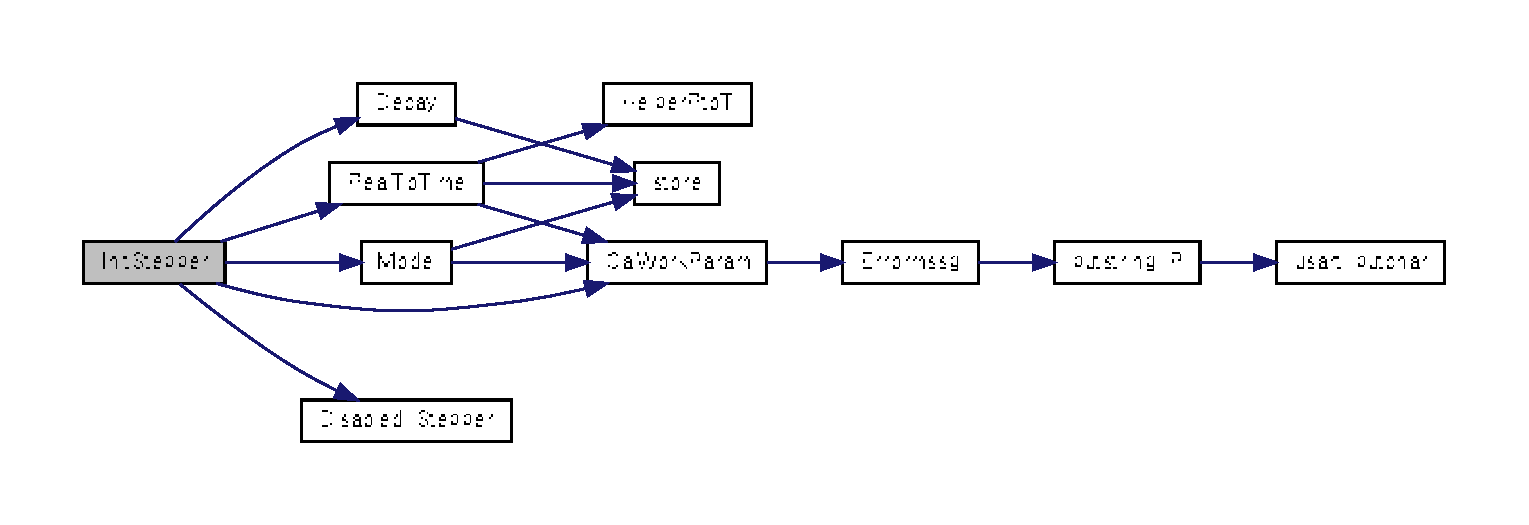
\includegraphics[width=350pt]{group__biba__drv_gad7c735bb7a3e49bba5cb72962f045d10_cgraph}
\end{center}
\end{figure}




Here is the caller graph for this function\-:
\nopagebreak
\begin{figure}[H]
\begin{center}
\leavevmode
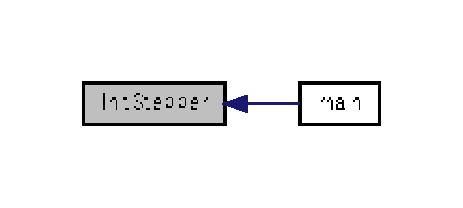
\includegraphics[width=222pt]{group__biba__drv_gad7c735bb7a3e49bba5cb72962f045d10_icgraph}
\end{center}
\end{figure}


\hypertarget{group__biba__drv_gafe73070875f7ba05536a1eeb83258c91}{\index{D\-R\-V8825 Library@{D\-R\-V8825 Library}!Mode@{Mode}}
\index{Mode@{Mode}!DRV8825 Library@{D\-R\-V8825 Library}}
\subsubsection[{Mode}]{\setlength{\rightskip}{0pt plus 5cm}void Mode (
\begin{DoxyParamCaption}
\item[{{\bf mode\-\_\-type}}]{mode}
\end{DoxyParamCaption}
)}}\label{group__biba__drv_gafe73070875f7ba05536a1eeb83258c91}
Function that sets the mode. \begin{DoxySeeAlso}{See Also}
\hyperlink{group__biba__drv_ga19269c193c0c4866cdc4e5abd433f9fc}{mode\-\_\-type} 
\end{DoxySeeAlso}

\begin{DoxyParams}{Parameters}
{\em mode} & the first argument. \\
\hline
\end{DoxyParams}
\begin{DoxyReturn}{Returns}
void 
\end{DoxyReturn}


Definition at line 215 of file drv\-\_\-8825.\-c.


\begin{DoxyCode}
216 \{
217     \hyperlink{drv__8825_8c_ab08e51d202664c8cc9434eac6c46f1f3}{CurrentMode} = mode;
218     \hyperlink{group__biba__drv_ga3389079a7106f1e741c0bc447dfbcbca}{CalWorkParam}( );
219     \hyperlink{group__biba__drv_gaaefaac2ed4c54f2008d8d236392c7261}{store}( );
220 
221     \textcolor{keywordflow}{if} ( mode == \hyperlink{group__biba__drv_gga19269c193c0c4866cdc4e5abd433f9fcaed3032a935a3b2a2ab90e2500dee1177}{MODE\_FULL\_STEP} )
222     \{
223         \hyperlink{group__biba__config_gaf2f231c38a29a96bac24f174fe7bf8b0}{clr\_bit}( \hyperlink{group__biba__config_gac31c37de4ad57d7e8e88d6a4ceb1a526}{PMODE0}, \hyperlink{group__biba__config_ga5daa4b780b82b5e8678d8c7095336b62}{MODE0} );
224         \hyperlink{group__biba__config_gaf2f231c38a29a96bac24f174fe7bf8b0}{clr\_bit}( \hyperlink{group__biba__config_gae2b3b81d452af91ecd26298a6a9954a8}{PMODE1}, \hyperlink{group__biba__config_ga443b1268c43b309560d57e34d50b5b3b}{MODE1} );
225         \hyperlink{group__biba__config_gaf2f231c38a29a96bac24f174fe7bf8b0}{clr\_bit}( \hyperlink{group__biba__config_ga4e6fd56609bbd34dc3797ee35d8610e8}{PMODE2}, \hyperlink{group__biba__config_gab2d8aca64e351712eae6f03e3f9d64ad}{MODE2} );
226     \}
227 
228     \textcolor{keywordflow}{if} ( mode == \hyperlink{group__biba__drv_gga19269c193c0c4866cdc4e5abd433f9fca7bf7cb276c55a5c4e13149d1e18b320f}{MODE\_HALF\_STEP} )
229     \{
230         \hyperlink{group__biba__config_ga4ee07d04aa2ef10d631d61c17c558464}{set\_bit}( \hyperlink{group__biba__config_gac31c37de4ad57d7e8e88d6a4ceb1a526}{PMODE0}, \hyperlink{group__biba__config_ga5daa4b780b82b5e8678d8c7095336b62}{MODE0} );
231         \hyperlink{group__biba__config_gaf2f231c38a29a96bac24f174fe7bf8b0}{clr\_bit}( \hyperlink{group__biba__config_gae2b3b81d452af91ecd26298a6a9954a8}{PMODE1}, \hyperlink{group__biba__config_ga443b1268c43b309560d57e34d50b5b3b}{MODE1} );
232         \hyperlink{group__biba__config_gaf2f231c38a29a96bac24f174fe7bf8b0}{clr\_bit}( \hyperlink{group__biba__config_ga4e6fd56609bbd34dc3797ee35d8610e8}{PMODE2}, \hyperlink{group__biba__config_gab2d8aca64e351712eae6f03e3f9d64ad}{MODE2} );
233     \}
234 
235     \textcolor{keywordflow}{if} ( mode == \hyperlink{group__biba__drv_gga19269c193c0c4866cdc4e5abd433f9fcaf16653dd137a6079ff5399de04861835}{MODE\_QUATER\_STEP} )
236     \{
237         \hyperlink{group__biba__config_gaf2f231c38a29a96bac24f174fe7bf8b0}{clr\_bit}( \hyperlink{group__biba__config_gac31c37de4ad57d7e8e88d6a4ceb1a526}{PMODE0}, \hyperlink{group__biba__config_ga5daa4b780b82b5e8678d8c7095336b62}{MODE0} );
238         \hyperlink{group__biba__config_ga4ee07d04aa2ef10d631d61c17c558464}{set\_bit}( \hyperlink{group__biba__config_gae2b3b81d452af91ecd26298a6a9954a8}{PMODE1}, \hyperlink{group__biba__config_ga443b1268c43b309560d57e34d50b5b3b}{MODE1} );
239         \hyperlink{group__biba__config_gaf2f231c38a29a96bac24f174fe7bf8b0}{clr\_bit}( \hyperlink{group__biba__config_ga4e6fd56609bbd34dc3797ee35d8610e8}{PMODE2}, \hyperlink{group__biba__config_gab2d8aca64e351712eae6f03e3f9d64ad}{MODE2} );
240     \}
241 
242     \textcolor{keywordflow}{if} ( mode == \hyperlink{group__biba__drv_gga19269c193c0c4866cdc4e5abd433f9fca4db57f4a88897e48818d92a223cd72d7}{MODE\_8\_MICROSTEP} )
243     \{
244         \hyperlink{group__biba__config_ga4ee07d04aa2ef10d631d61c17c558464}{set\_bit}( \hyperlink{group__biba__config_gac31c37de4ad57d7e8e88d6a4ceb1a526}{PMODE0}, \hyperlink{group__biba__config_ga5daa4b780b82b5e8678d8c7095336b62}{MODE0} );
245         \hyperlink{group__biba__config_ga4ee07d04aa2ef10d631d61c17c558464}{set\_bit}( \hyperlink{group__biba__config_gae2b3b81d452af91ecd26298a6a9954a8}{PMODE1}, \hyperlink{group__biba__config_ga443b1268c43b309560d57e34d50b5b3b}{MODE1} );
246         \hyperlink{group__biba__config_gaf2f231c38a29a96bac24f174fe7bf8b0}{clr\_bit}( \hyperlink{group__biba__config_ga4e6fd56609bbd34dc3797ee35d8610e8}{PMODE2}, \hyperlink{group__biba__config_gab2d8aca64e351712eae6f03e3f9d64ad}{MODE2} );
247     \}
248 
249     \textcolor{keywordflow}{if} ( mode == \hyperlink{group__biba__drv_gga19269c193c0c4866cdc4e5abd433f9fcac75bcca2721976d5185711ca481ccbb0}{MODE\_16\_MICROSTEP} )
250     \{
251         \hyperlink{group__biba__config_gaf2f231c38a29a96bac24f174fe7bf8b0}{clr\_bit}( \hyperlink{group__biba__config_gac31c37de4ad57d7e8e88d6a4ceb1a526}{PMODE0}, \hyperlink{group__biba__config_ga5daa4b780b82b5e8678d8c7095336b62}{MODE0} );
252         \hyperlink{group__biba__config_gaf2f231c38a29a96bac24f174fe7bf8b0}{clr\_bit}( \hyperlink{group__biba__config_gae2b3b81d452af91ecd26298a6a9954a8}{PMODE1}, \hyperlink{group__biba__config_ga443b1268c43b309560d57e34d50b5b3b}{MODE1} );
253         \hyperlink{group__biba__config_ga4ee07d04aa2ef10d631d61c17c558464}{set\_bit}( \hyperlink{group__biba__config_ga4e6fd56609bbd34dc3797ee35d8610e8}{PMODE2}, \hyperlink{group__biba__config_gab2d8aca64e351712eae6f03e3f9d64ad}{MODE2} );
254     \}
255 
256     \textcolor{keywordflow}{if} ( mode == \hyperlink{group__biba__drv_gga19269c193c0c4866cdc4e5abd433f9fcacb3d9ffb67d18343290fe5474bc1b4d5}{MODE\_32\_MICROSTEP} )
257     \{
258         \hyperlink{group__biba__config_ga4ee07d04aa2ef10d631d61c17c558464}{set\_bit}( \hyperlink{group__biba__config_gac31c37de4ad57d7e8e88d6a4ceb1a526}{PMODE0}, \hyperlink{group__biba__config_ga5daa4b780b82b5e8678d8c7095336b62}{MODE0} );
259         \hyperlink{group__biba__config_gaf2f231c38a29a96bac24f174fe7bf8b0}{clr\_bit}( \hyperlink{group__biba__config_gae2b3b81d452af91ecd26298a6a9954a8}{PMODE1}, \hyperlink{group__biba__config_ga443b1268c43b309560d57e34d50b5b3b}{MODE1} );
260         \hyperlink{group__biba__config_ga4ee07d04aa2ef10d631d61c17c558464}{set\_bit}( \hyperlink{group__biba__config_ga4e6fd56609bbd34dc3797ee35d8610e8}{PMODE2}, \hyperlink{group__biba__config_gab2d8aca64e351712eae6f03e3f9d64ad}{MODE2} );
261     \}
262 
263 \}
\end{DoxyCode}


Here is the call graph for this function\-:
\nopagebreak
\begin{figure}[H]
\begin{center}
\leavevmode
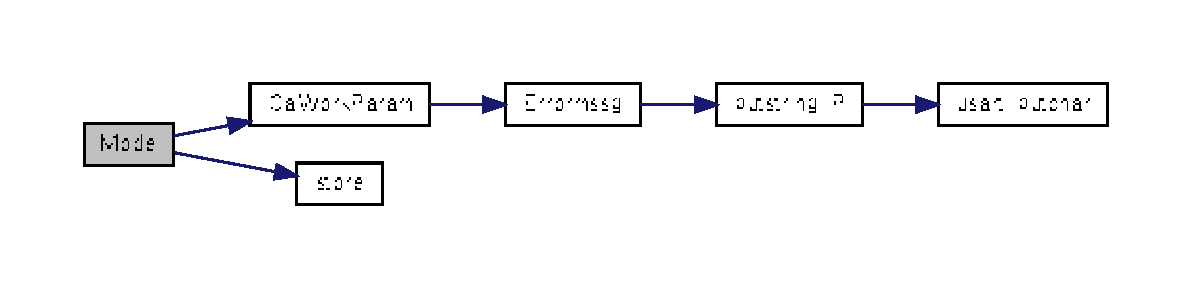
\includegraphics[width=350pt]{group__biba__drv_gafe73070875f7ba05536a1eeb83258c91_cgraph}
\end{center}
\end{figure}




Here is the caller graph for this function\-:
\nopagebreak
\begin{figure}[H]
\begin{center}
\leavevmode
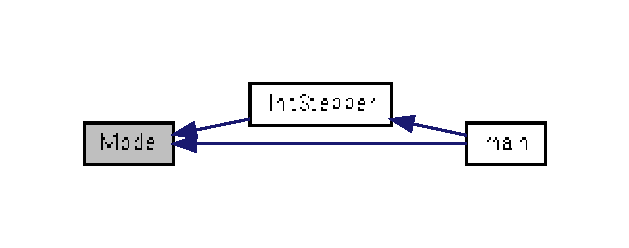
\includegraphics[width=302pt]{group__biba__drv_gafe73070875f7ba05536a1eeb83258c91_icgraph}
\end{center}
\end{figure}


\hypertarget{group__biba__drv_gad23127bea36c997c0b1c767f2421db6a}{\index{D\-R\-V8825 Library@{D\-R\-V8825 Library}!Real\-To\-Time@{Real\-To\-Time}}
\index{Real\-To\-Time@{Real\-To\-Time}!DRV8825 Library@{D\-R\-V8825 Library}}
\subsubsection[{Real\-To\-Time}]{\setlength{\rightskip}{0pt plus 5cm}void Real\-To\-Time (
\begin{DoxyParamCaption}
\item[{void}]{}
\end{DoxyParamCaption}
)}}\label{group__biba__drv_gad23127bea36c997c0b1c767f2421db6a}
Calculates the real speed to the timmer speed. \begin{DoxyReturn}{Returns}
void 
\end{DoxyReturn}


Definition at line 622 of file drv\-\_\-8825.\-c.


\begin{DoxyCode}
623 \{
624     
625     uint16\_t revpermin;
626     \hyperlink{drv__8825_8c_a7d20b8cec6f96108790d4bf76b9c469d}{TimeParam}.\hyperlink{structMotor__Parameters_a501458e333945f49f03c295e2f49e3b9}{MaxSpeed}=\hyperlink{group__biba__drv_ga8f3808b2e4aa3b2a8f6467a2aaa31995}{HelperRtoT}(\hyperlink{drv__8825_8c_a2e720ed1ed0ef90dba27c1f246048dcd}{RealSpeed}.
      \hyperlink{structMotor__Parameters_a501458e333945f49f03c295e2f49e3b9}{MaxSpeed});
627     \hyperlink{drv__8825_8c_a7d20b8cec6f96108790d4bf76b9c469d}{TimeParam}.\hyperlink{structMotor__Parameters_aaf0ac3ed818f5c89cc86ea1d9174dc43}{MinSpeed}=\hyperlink{group__biba__drv_ga8f3808b2e4aa3b2a8f6467a2aaa31995}{HelperRtoT}(\hyperlink{drv__8825_8c_a2e720ed1ed0ef90dba27c1f246048dcd}{RealSpeed}.
      \hyperlink{structMotor__Parameters_aaf0ac3ed818f5c89cc86ea1d9174dc43}{MinSpeed});
628     
629     revpermin = ( \hyperlink{drv__8825_8c_a7d20b8cec6f96108790d4bf76b9c469d}{TimeParam}.\hyperlink{structMotor__Parameters_aaf0ac3ed818f5c89cc86ea1d9174dc43}{MinSpeed} - \hyperlink{drv__8825_8c_a7d20b8cec6f96108790d4bf76b9c469d}{TimeParam}.
      \hyperlink{structMotor__Parameters_a501458e333945f49f03c295e2f49e3b9}{MaxSpeed} ) / \hyperlink{drv__8825_8c_a2e720ed1ed0ef90dba27c1f246048dcd}{RealSpeed}.\hyperlink{structMotor__Parameters_aa9f1146edc6d945d535eec80a01481f1}{Acceleration};
630 
631     \textcolor{comment}{//putstring\_P( PSTR( "acc=" ) );}
632     \textcolor{comment}{//putstring( int\_to\_string( ( uint64\_t ) ( revpermin ) ) );}
633     \textcolor{comment}{//putstring\_P( PSTR( "\(\backslash\)r" ) );}
634 
635     if ( revpermin < 1 )
636     \{
637         \hyperlink{drv__8825_8c_a7d20b8cec6f96108790d4bf76b9c469d}{TimeParam}.\hyperlink{structMotor__Parameters_aa9f1146edc6d945d535eec80a01481f1}{Acceleration} = 1;
638         \textcolor{comment}{//  putstring\_P( PSTR( "Acc  low\(\backslash\)r" ) );}
639     \} \textcolor{keywordflow}{else}
640     \{
641         \hyperlink{drv__8825_8c_a7d20b8cec6f96108790d4bf76b9c469d}{TimeParam}.\hyperlink{structMotor__Parameters_aa9f1146edc6d945d535eec80a01481f1}{Acceleration} = revpermin;
642     \}
643 
644     \hyperlink{group__biba__drv_ga3389079a7106f1e741c0bc447dfbcbca}{CalWorkParam}( );
645     \hyperlink{group__biba__drv_gaaefaac2ed4c54f2008d8d236392c7261}{store}( );
646 \}
\end{DoxyCode}


Here is the call graph for this function\-:
\nopagebreak
\begin{figure}[H]
\begin{center}
\leavevmode
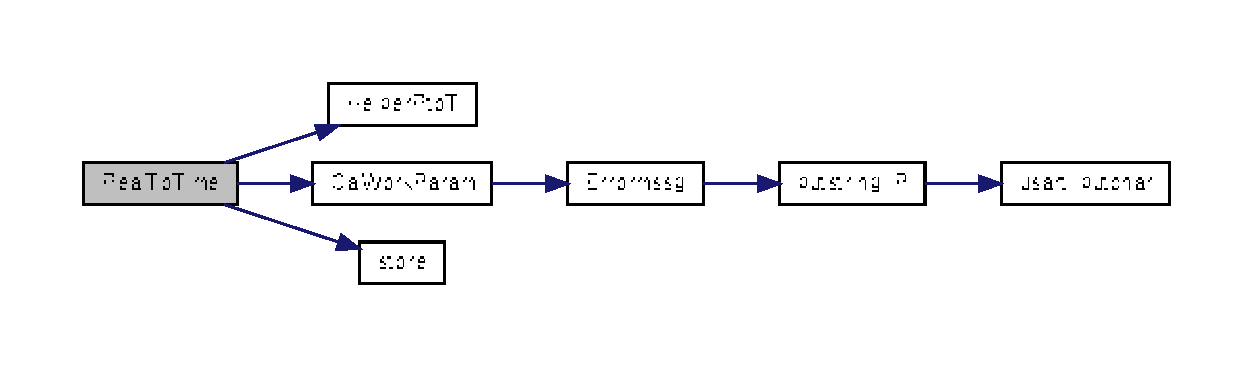
\includegraphics[width=350pt]{group__biba__drv_gad23127bea36c997c0b1c767f2421db6a_cgraph}
\end{center}
\end{figure}




Here is the caller graph for this function\-:
\nopagebreak
\begin{figure}[H]
\begin{center}
\leavevmode
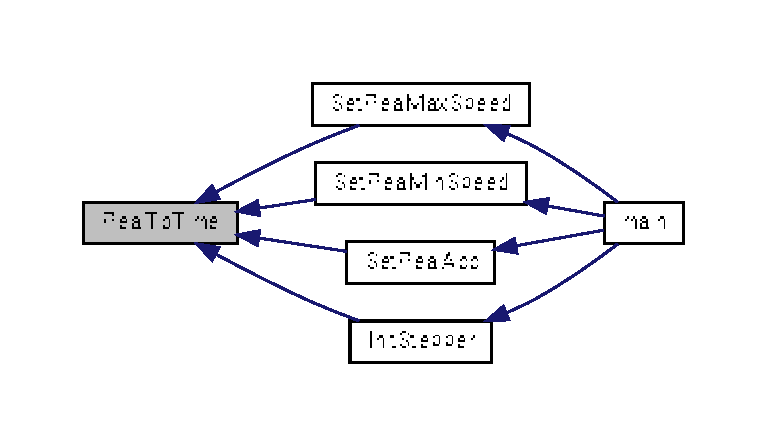
\includegraphics[width=350pt]{group__biba__drv_gad23127bea36c997c0b1c767f2421db6a_icgraph}
\end{center}
\end{figure}


\hypertarget{group__biba__drv_ga0c630286eeb4f2b49bfe96670dafd65c}{\index{D\-R\-V8825 Library@{D\-R\-V8825 Library}!Set\-\_\-\-Steps\-\_\-revol@{Set\-\_\-\-Steps\-\_\-revol}}
\index{Set\-\_\-\-Steps\-\_\-revol@{Set\-\_\-\-Steps\-\_\-revol}!DRV8825 Library@{D\-R\-V8825 Library}}
\subsubsection[{Set\-\_\-\-Steps\-\_\-revol}]{\setlength{\rightskip}{0pt plus 5cm}void Set\-\_\-\-Steps\-\_\-revol (
\begin{DoxyParamCaption}
\item[{uint16\-\_\-t}]{step\-\_\-rev}
\end{DoxyParamCaption}
)}}\label{group__biba__drv_ga0c630286eeb4f2b49bfe96670dafd65c}
Sets the steps per revolution. \begin{DoxySeeAlso}{See Also}
\hyperlink{drv__8825_8c_a54128bfe0cfae9cbd8577cf456951f21}{Steps\-Per\-Rev} 
\end{DoxySeeAlso}

\begin{DoxyParams}{Parameters}
{\em step\-\_\-rev} & the first argument. \\
\hline
\end{DoxyParams}
\begin{DoxyReturn}{Returns}
void 
\end{DoxyReturn}


Definition at line 535 of file drv\-\_\-8825.\-c.


\begin{DoxyCode}
536 \{
537     \hyperlink{drv__8825_8c_a54128bfe0cfae9cbd8577cf456951f21}{StepsPerRev} = step\_rev;
538 \}
\end{DoxyCode}


Here is the caller graph for this function\-:
\nopagebreak
\begin{figure}[H]
\begin{center}
\leavevmode
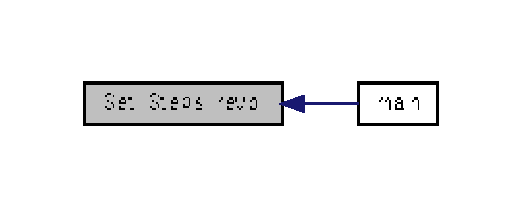
\includegraphics[width=250pt]{group__biba__drv_ga0c630286eeb4f2b49bfe96670dafd65c_icgraph}
\end{center}
\end{figure}


\hypertarget{group__biba__drv_ga746cb11e60c877a82b3ecbdbaa375f5e}{\index{D\-R\-V8825 Library@{D\-R\-V8825 Library}!Set\-Acceleration@{Set\-Acceleration}}
\index{Set\-Acceleration@{Set\-Acceleration}!DRV8825 Library@{D\-R\-V8825 Library}}
\subsubsection[{Set\-Acceleration}]{\setlength{\rightskip}{0pt plus 5cm}void Set\-Acceleration (
\begin{DoxyParamCaption}
\item[{uint16\-\_\-t}]{accel}
\end{DoxyParamCaption}
)}}\label{group__biba__drv_ga746cb11e60c877a82b3ecbdbaa375f5e}
Function that sets the acceleration. \begin{DoxySeeAlso}{See Also}
Time\-Param.\-Acceleration 
\end{DoxySeeAlso}

\begin{DoxyParams}{Parameters}
{\em accel} & the first argument. \\
\hline
\end{DoxyParams}
\begin{DoxyReturn}{Returns}
void 
\end{DoxyReturn}


Definition at line 153 of file drv\-\_\-8825.\-c.


\begin{DoxyCode}
154 \{
155     \hyperlink{drv__8825_8c_a7d20b8cec6f96108790d4bf76b9c469d}{TimeParam}.\hyperlink{structMotor__Parameters_aa9f1146edc6d945d535eec80a01481f1}{Acceleration} = accel;
156     \hyperlink{group__biba__drv_gaec239a01fef85140bc7c12fa612f421b}{TimeToReal}( );
157 \}
\end{DoxyCode}


Here is the call graph for this function\-:
\nopagebreak
\begin{figure}[H]
\begin{center}
\leavevmode
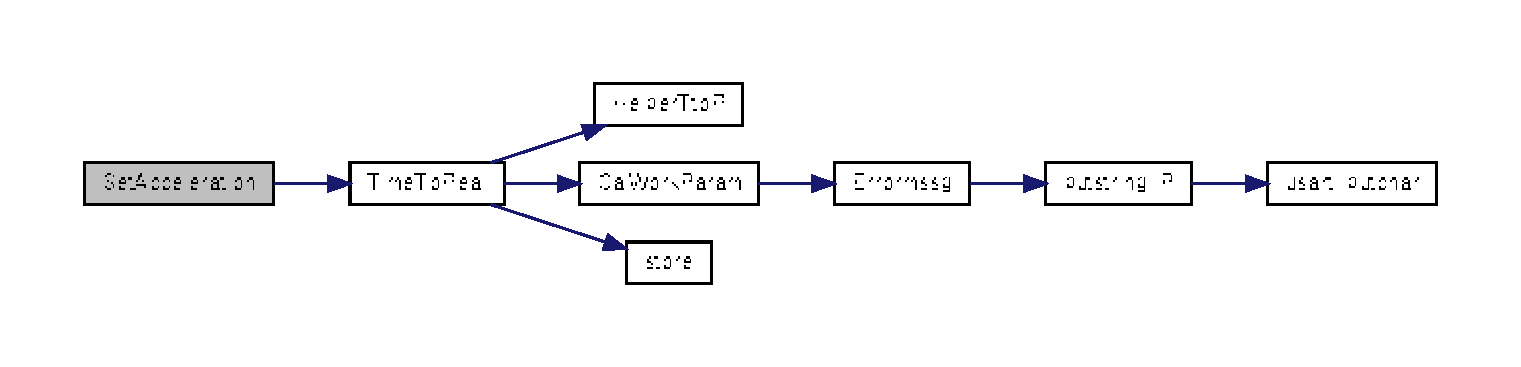
\includegraphics[width=350pt]{group__biba__drv_ga746cb11e60c877a82b3ecbdbaa375f5e_cgraph}
\end{center}
\end{figure}




Here is the caller graph for this function\-:
\nopagebreak
\begin{figure}[H]
\begin{center}
\leavevmode
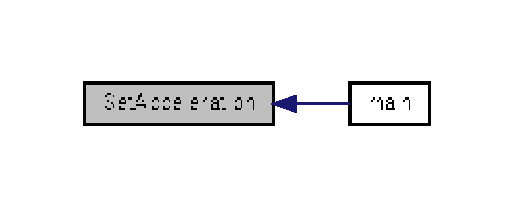
\includegraphics[width=246pt]{group__biba__drv_ga746cb11e60c877a82b3ecbdbaa375f5e_icgraph}
\end{center}
\end{figure}


\hypertarget{group__biba__drv_ga91f64f1e8f2b67bfcf24f6d2a2249373}{\index{D\-R\-V8825 Library@{D\-R\-V8825 Library}!Set\-Current\-Speed@{Set\-Current\-Speed}}
\index{Set\-Current\-Speed@{Set\-Current\-Speed}!DRV8825 Library@{D\-R\-V8825 Library}}
\subsubsection[{Set\-Current\-Speed}]{\setlength{\rightskip}{0pt plus 5cm}void Set\-Current\-Speed (
\begin{DoxyParamCaption}
\item[{uint16\-\_\-t}]{spd}
\end{DoxyParamCaption}
)}}\label{group__biba__drv_ga91f64f1e8f2b67bfcf24f6d2a2249373}
Sets the current speed. \begin{DoxySeeAlso}{See Also}
\hyperlink{structMotion_a50860ebd661de5d104a36a92cd5f17c7}{Motion.\-Current\-Speed} 
\end{DoxySeeAlso}

\begin{DoxyParams}{Parameters}
{\em spd} & the first argument. \\
\hline
\end{DoxyParams}
\begin{DoxyReturn}{Returns}
void 
\end{DoxyReturn}


Definition at line 468 of file drv\-\_\-8825.\-c.


\begin{DoxyCode}
469 \{
470     \hyperlink{structMotion}{Motion}.\hyperlink{structMotion_a50860ebd661de5d104a36a92cd5f17c7}{CurrentSpeed} = spd;
471 \}
\end{DoxyCode}
\hypertarget{group__biba__drv_gaf56c9e829e6f40a75e89bd16f5051c63}{\index{D\-R\-V8825 Library@{D\-R\-V8825 Library}!Set\-Max\-Speed@{Set\-Max\-Speed}}
\index{Set\-Max\-Speed@{Set\-Max\-Speed}!DRV8825 Library@{D\-R\-V8825 Library}}
\subsubsection[{Set\-Max\-Speed}]{\setlength{\rightskip}{0pt plus 5cm}void Set\-Max\-Speed (
\begin{DoxyParamCaption}
\item[{uint16\-\_\-t}]{spd}
\end{DoxyParamCaption}
)}}\label{group__biba__drv_gaf56c9e829e6f40a75e89bd16f5051c63}
Function that sets the maximum speed. \begin{DoxySeeAlso}{See Also}
Time\-Param.\-Max\-Speed 
\end{DoxySeeAlso}

\begin{DoxyParams}{Parameters}
{\em spd} & the first argument. \\
\hline
\end{DoxyParams}
\begin{DoxyReturn}{Returns}
void 
\end{DoxyReturn}


Definition at line 128 of file drv\-\_\-8825.\-c.


\begin{DoxyCode}
129 \{
130     \hyperlink{drv__8825_8c_a7d20b8cec6f96108790d4bf76b9c469d}{TimeParam}.\hyperlink{structMotor__Parameters_a501458e333945f49f03c295e2f49e3b9}{MaxSpeed} = spd;
131     \hyperlink{group__biba__drv_gaec239a01fef85140bc7c12fa612f421b}{TimeToReal}( );
132 \}
\end{DoxyCode}


Here is the call graph for this function\-:
\nopagebreak
\begin{figure}[H]
\begin{center}
\leavevmode
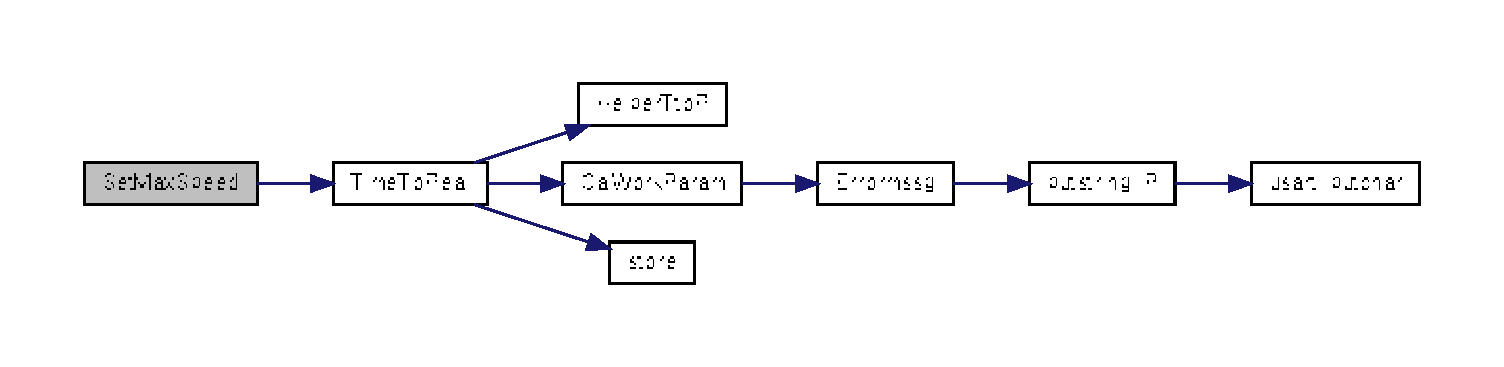
\includegraphics[width=350pt]{group__biba__drv_gaf56c9e829e6f40a75e89bd16f5051c63_cgraph}
\end{center}
\end{figure}




Here is the caller graph for this function\-:
\nopagebreak
\begin{figure}[H]
\begin{center}
\leavevmode
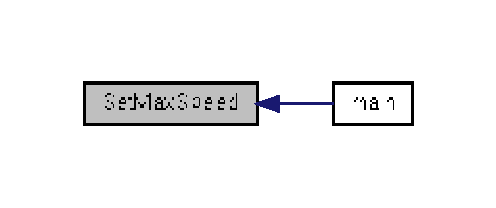
\includegraphics[width=238pt]{group__biba__drv_gaf56c9e829e6f40a75e89bd16f5051c63_icgraph}
\end{center}
\end{figure}


\hypertarget{group__biba__drv_ga39d145b6dc7b1fa19582960613440fd4}{\index{D\-R\-V8825 Library@{D\-R\-V8825 Library}!Set\-Min\-Speed@{Set\-Min\-Speed}}
\index{Set\-Min\-Speed@{Set\-Min\-Speed}!DRV8825 Library@{D\-R\-V8825 Library}}
\subsubsection[{Set\-Min\-Speed}]{\setlength{\rightskip}{0pt plus 5cm}void Set\-Min\-Speed (
\begin{DoxyParamCaption}
\item[{uint16\-\_\-t}]{spd}
\end{DoxyParamCaption}
)}}\label{group__biba__drv_ga39d145b6dc7b1fa19582960613440fd4}
Function that sets the minimum speed. \begin{DoxySeeAlso}{See Also}
Time\-Param.\-Min\-Speed 
\end{DoxySeeAlso}

\begin{DoxyParams}{Parameters}
{\em spd} & the first argument. \\
\hline
\end{DoxyParams}
\begin{DoxyReturn}{Returns}
void 
\end{DoxyReturn}


Definition at line 141 of file drv\-\_\-8825.\-c.


\begin{DoxyCode}
142 \{
143     \hyperlink{drv__8825_8c_a7d20b8cec6f96108790d4bf76b9c469d}{TimeParam}.\hyperlink{structMotor__Parameters_aaf0ac3ed818f5c89cc86ea1d9174dc43}{MinSpeed} = spd;
144     \hyperlink{group__biba__drv_gaec239a01fef85140bc7c12fa612f421b}{TimeToReal}( );
145 \}
\end{DoxyCode}


Here is the call graph for this function\-:
\nopagebreak
\begin{figure}[H]
\begin{center}
\leavevmode
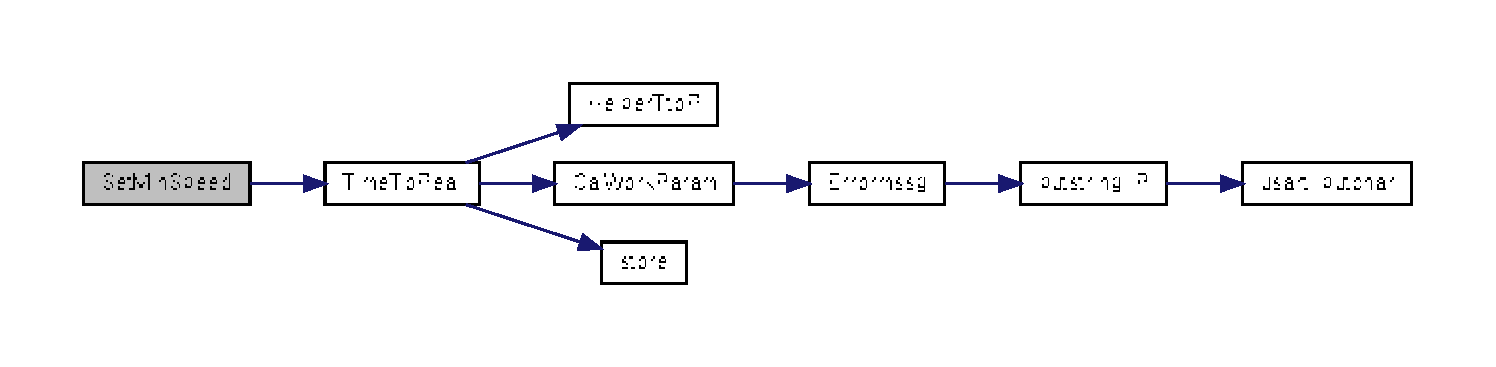
\includegraphics[width=350pt]{group__biba__drv_ga39d145b6dc7b1fa19582960613440fd4_cgraph}
\end{center}
\end{figure}




Here is the caller graph for this function\-:
\nopagebreak
\begin{figure}[H]
\begin{center}
\leavevmode
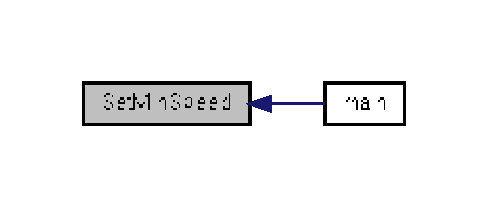
\includegraphics[width=234pt]{group__biba__drv_ga39d145b6dc7b1fa19582960613440fd4_icgraph}
\end{center}
\end{figure}


\hypertarget{group__biba__drv_gaf272b22659980a7a5b9be13378963f67}{\index{D\-R\-V8825 Library@{D\-R\-V8825 Library}!Set\-Real\-Acc@{Set\-Real\-Acc}}
\index{Set\-Real\-Acc@{Set\-Real\-Acc}!DRV8825 Library@{D\-R\-V8825 Library}}
\subsubsection[{Set\-Real\-Acc}]{\setlength{\rightskip}{0pt plus 5cm}void Set\-Real\-Acc (
\begin{DoxyParamCaption}
\item[{uint16\-\_\-t}]{realacc}
\end{DoxyParamCaption}
)}}\label{group__biba__drv_gaf272b22659980a7a5b9be13378963f67}
Sets the real acceleration. \begin{DoxySeeAlso}{See Also}
Real\-Speed.\-Acceleration 
\end{DoxySeeAlso}

\begin{DoxyParams}{Parameters}
{\em realacc} & the first argument. \\
\hline
\end{DoxyParams}
\begin{DoxyReturn}{Returns}
void 
\end{DoxyReturn}


Definition at line 581 of file drv\-\_\-8825.\-c.


\begin{DoxyCode}
582 \{
583     \hyperlink{drv__8825_8c_a2e720ed1ed0ef90dba27c1f246048dcd}{RealSpeed}.\hyperlink{structMotor__Parameters_aa9f1146edc6d945d535eec80a01481f1}{Acceleration} = realacc;
584     \hyperlink{group__biba__drv_gad23127bea36c997c0b1c767f2421db6a}{RealToTime}( );
585 \}
\end{DoxyCode}


Here is the call graph for this function\-:
\nopagebreak
\begin{figure}[H]
\begin{center}
\leavevmode
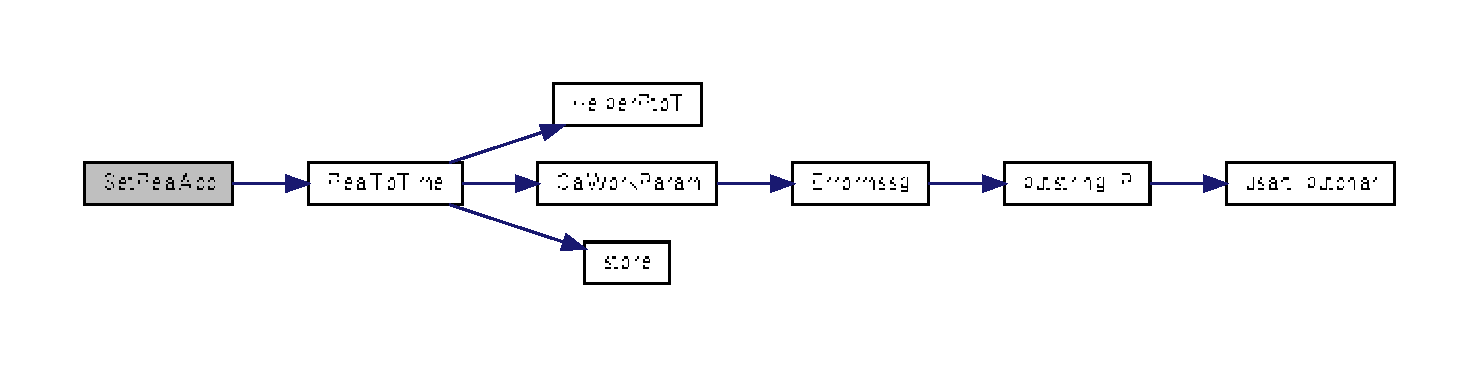
\includegraphics[width=350pt]{group__biba__drv_gaf272b22659980a7a5b9be13378963f67_cgraph}
\end{center}
\end{figure}




Here is the caller graph for this function\-:
\nopagebreak
\begin{figure}[H]
\begin{center}
\leavevmode
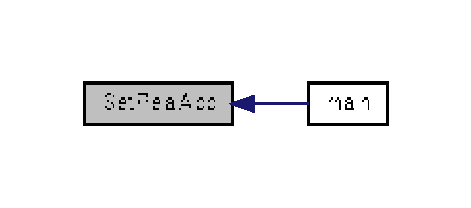
\includegraphics[width=226pt]{group__biba__drv_gaf272b22659980a7a5b9be13378963f67_icgraph}
\end{center}
\end{figure}


\hypertarget{group__biba__drv_ga544f7d7cdcd1fc93afaaa833d1086654}{\index{D\-R\-V8825 Library@{D\-R\-V8825 Library}!Set\-Real\-Max\-Speed@{Set\-Real\-Max\-Speed}}
\index{Set\-Real\-Max\-Speed@{Set\-Real\-Max\-Speed}!DRV8825 Library@{D\-R\-V8825 Library}}
\subsubsection[{Set\-Real\-Max\-Speed}]{\setlength{\rightskip}{0pt plus 5cm}void Set\-Real\-Max\-Speed (
\begin{DoxyParamCaption}
\item[{uint16\-\_\-t}]{maxspd}
\end{DoxyParamCaption}
)}}\label{group__biba__drv_ga544f7d7cdcd1fc93afaaa833d1086654}
Sets the real maximum speed. \begin{DoxySeeAlso}{See Also}
Real\-Speed.\-Max\-Speed 
\end{DoxySeeAlso}

\begin{DoxyParams}{Parameters}
{\em maxspd} & the first argument. \\
\hline
\end{DoxyParams}
\begin{DoxyReturn}{Returns}
void 
\end{DoxyReturn}


Definition at line 557 of file drv\-\_\-8825.\-c.


\begin{DoxyCode}
558 \{
559     \hyperlink{drv__8825_8c_a2e720ed1ed0ef90dba27c1f246048dcd}{RealSpeed}.\hyperlink{structMotor__Parameters_a501458e333945f49f03c295e2f49e3b9}{MaxSpeed} = maxspd;
560     \hyperlink{group__biba__drv_gad23127bea36c997c0b1c767f2421db6a}{RealToTime}( );
561 \}
\end{DoxyCode}


Here is the call graph for this function\-:
\nopagebreak
\begin{figure}[H]
\begin{center}
\leavevmode
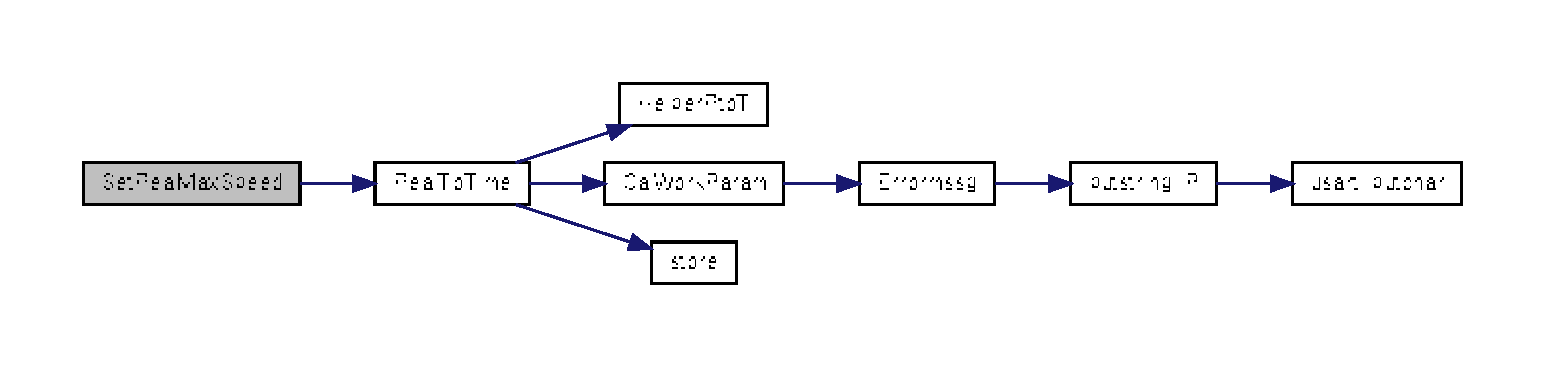
\includegraphics[width=350pt]{group__biba__drv_ga544f7d7cdcd1fc93afaaa833d1086654_cgraph}
\end{center}
\end{figure}




Here is the caller graph for this function\-:
\nopagebreak
\begin{figure}[H]
\begin{center}
\leavevmode
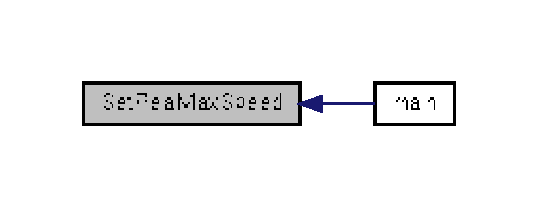
\includegraphics[width=258pt]{group__biba__drv_ga544f7d7cdcd1fc93afaaa833d1086654_icgraph}
\end{center}
\end{figure}


\hypertarget{group__biba__drv_gaf589e1659ecdbe47a83571e1368dc0e2}{\index{D\-R\-V8825 Library@{D\-R\-V8825 Library}!Set\-Real\-Min\-Speed@{Set\-Real\-Min\-Speed}}
\index{Set\-Real\-Min\-Speed@{Set\-Real\-Min\-Speed}!DRV8825 Library@{D\-R\-V8825 Library}}
\subsubsection[{Set\-Real\-Min\-Speed}]{\setlength{\rightskip}{0pt plus 5cm}void Set\-Real\-Min\-Speed (
\begin{DoxyParamCaption}
\item[{uint16\-\_\-t}]{minspd}
\end{DoxyParamCaption}
)}}\label{group__biba__drv_gaf589e1659ecdbe47a83571e1368dc0e2}
Sets the real minimum speed. \begin{DoxySeeAlso}{See Also}
Real\-Speed.\-Min\-Speed 
\end{DoxySeeAlso}

\begin{DoxyParams}{Parameters}
{\em minspd} & the first argument. \\
\hline
\end{DoxyParams}
\begin{DoxyReturn}{Returns}
void 
\end{DoxyReturn}


Definition at line 569 of file drv\-\_\-8825.\-c.


\begin{DoxyCode}
570 \{
571     \hyperlink{drv__8825_8c_a2e720ed1ed0ef90dba27c1f246048dcd}{RealSpeed}.\hyperlink{structMotor__Parameters_aaf0ac3ed818f5c89cc86ea1d9174dc43}{MinSpeed} = minspd;
572     \hyperlink{group__biba__drv_gad23127bea36c997c0b1c767f2421db6a}{RealToTime}( );
573 \}
\end{DoxyCode}


Here is the call graph for this function\-:
\nopagebreak
\begin{figure}[H]
\begin{center}
\leavevmode
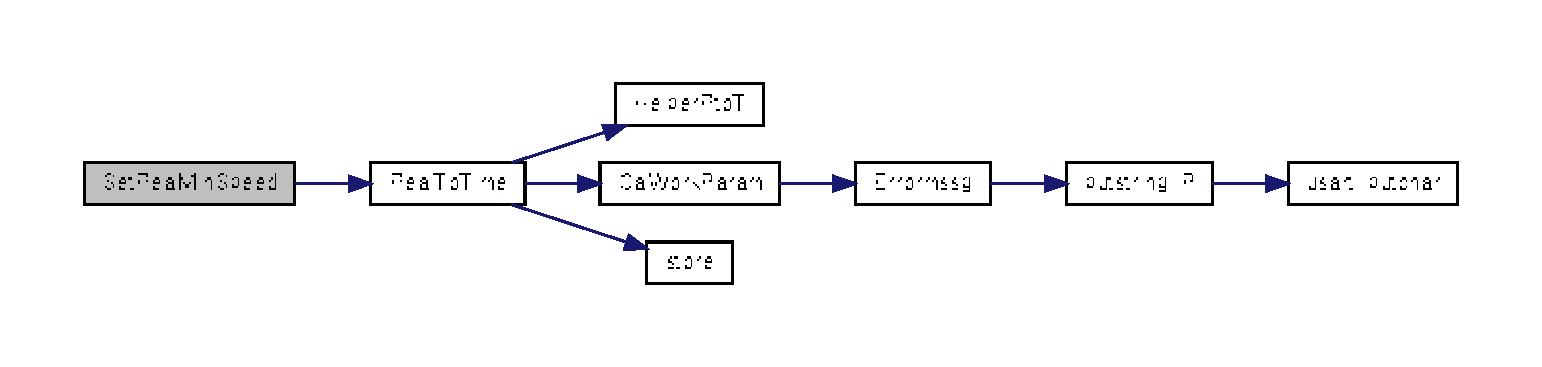
\includegraphics[width=350pt]{group__biba__drv_gaf589e1659ecdbe47a83571e1368dc0e2_cgraph}
\end{center}
\end{figure}




Here is the caller graph for this function\-:
\nopagebreak
\begin{figure}[H]
\begin{center}
\leavevmode
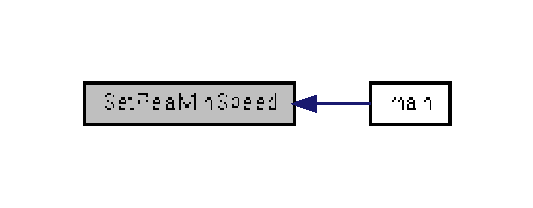
\includegraphics[width=256pt]{group__biba__drv_gaf589e1659ecdbe47a83571e1368dc0e2_icgraph}
\end{center}
\end{figure}


\hypertarget{group__biba__drv_ga7920069eba0a349a19a7e5af32321ad8}{\index{D\-R\-V8825 Library@{D\-R\-V8825 Library}!Step@{Step}}
\index{Step@{Step}!DRV8825 Library@{D\-R\-V8825 Library}}
\subsubsection[{Step}]{\setlength{\rightskip}{0pt plus 5cm}void Step (
\begin{DoxyParamCaption}
\item[{{\bf step\-\_\-type}}]{step}
\end{DoxyParamCaption}
)}}\label{group__biba__drv_ga7920069eba0a349a19a7e5af32321ad8}
Performs single step. \begin{DoxySeeAlso}{See Also}
\hyperlink{group__biba__drv_ga3af682b92aa259509aea217f6dc64356}{step\-\_\-type} 
\end{DoxySeeAlso}

\begin{DoxyParams}{Parameters}
{\em step} & the first argument. \\
\hline
\end{DoxyParams}
\begin{DoxyReturn}{Returns}
void 
\end{DoxyReturn}


Definition at line 272 of file drv\-\_\-8825.\-c.


\begin{DoxyCode}
273 \{
274     \textcolor{keywordflow}{if} ( step == \hyperlink{group__biba__drv_gga3af682b92aa259509aea217f6dc64356aafe6025725d6001f0b0a973f1e719cc4}{STEP\_CLOCKWISE} )
275     \{
276         \hyperlink{group__biba__config_ga4ee07d04aa2ef10d631d61c17c558464}{set\_bit}( \hyperlink{group__biba__config_ga27c908eae571c75c5a5e37d6fcc8db9d}{PDIRECTION}, \hyperlink{group__biba__config_ga1d692daf1ffadae2243a5ab556589629}{DIRECTION} );
277 
278     \} \textcolor{keywordflow}{else}
279     \{
280         \hyperlink{group__biba__config_gaf2f231c38a29a96bac24f174fe7bf8b0}{clr\_bit}( \hyperlink{group__biba__config_ga27c908eae571c75c5a5e37d6fcc8db9d}{PDIRECTION}, \hyperlink{group__biba__config_ga1d692daf1ffadae2243a5ab556589629}{DIRECTION} );
281     \}
282     \hyperlink{group__biba__config_ga4ee07d04aa2ef10d631d61c17c558464}{set\_bit}( \hyperlink{group__biba__config_gaa3a1d04d71d6791ec7d5d9bd6d2d8cb1}{PSTEP}, \hyperlink{group__biba__config_ga70be2dc5c8bdc85b027ea6118753cca1}{STEP} );
283     \_delay\_us( 2 );
284     \hyperlink{group__biba__config_gaf2f231c38a29a96bac24f174fe7bf8b0}{clr\_bit}( \hyperlink{group__biba__config_gaa3a1d04d71d6791ec7d5d9bd6d2d8cb1}{PSTEP}, \hyperlink{group__biba__config_ga70be2dc5c8bdc85b027ea6118753cca1}{STEP} );
285     \_delay\_us( 2 );
286 \}
\end{DoxyCode}


Here is the caller graph for this function\-:
\nopagebreak
\begin{figure}[H]
\begin{center}
\leavevmode
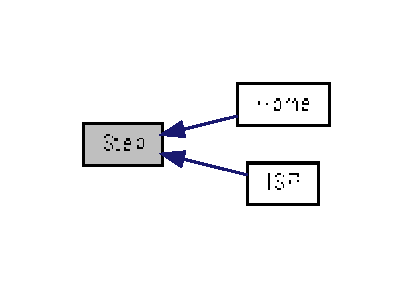
\includegraphics[width=198pt]{group__biba__drv_ga7920069eba0a349a19a7e5af32321ad8_icgraph}
\end{center}
\end{figure}


\hypertarget{group__biba__drv_ga1db502f9943a62943380a04ba0bd52cb}{\index{D\-R\-V8825 Library@{D\-R\-V8825 Library}!Stop\-\_\-\-Motion\-\_\-fast@{Stop\-\_\-\-Motion\-\_\-fast}}
\index{Stop\-\_\-\-Motion\-\_\-fast@{Stop\-\_\-\-Motion\-\_\-fast}!DRV8825 Library@{D\-R\-V8825 Library}}
\subsubsection[{Stop\-\_\-\-Motion\-\_\-fast}]{\setlength{\rightskip}{0pt plus 5cm}void Stop\-\_\-\-Motion\-\_\-fast (
\begin{DoxyParamCaption}
\item[{void}]{}
\end{DoxyParamCaption}
)}}\label{group__biba__drv_ga1db502f9943a62943380a04ba0bd52cb}
Stops the movement without deacceleration at the end. \begin{DoxyReturn}{Returns}
void 
\end{DoxyReturn}


Definition at line 361 of file drv\-\_\-8825.\-c.


\begin{DoxyCode}
362 \{
363     \hyperlink{drv__8825_8c_a295a33258d6c0cfd0dd62f0574952f21}{ConstSpd} = 0;
364     \hyperlink{structMotion}{Motion}.\hyperlink{structMotion_a970d0810aac5cab75c8dd0c95e4473da}{StepsAccel} = 0;
365     \hyperlink{structMotion}{Motion}.\hyperlink{structMotion_aa99fa8cb04ab25fc08e7b65664b7fdef}{StepsConstSpeed} = 0;
366     \hyperlink{structMotion}{Motion}.\hyperlink{structMotion_a0d7942de8bba5304852a9f2d8fe833e5}{StepsDeaccel} = 0;
367 \}
\end{DoxyCode}


Here is the caller graph for this function\-:
\nopagebreak
\begin{figure}[H]
\begin{center}
\leavevmode
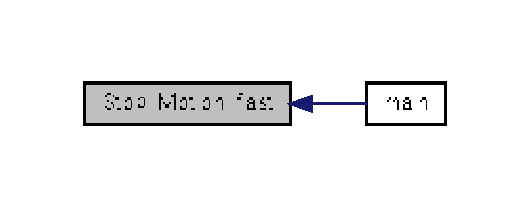
\includegraphics[width=254pt]{group__biba__drv_ga1db502f9943a62943380a04ba0bd52cb_icgraph}
\end{center}
\end{figure}


\hypertarget{group__biba__drv_ga95c2965416e69e644b9f5a482707ae9f}{\index{D\-R\-V8825 Library@{D\-R\-V8825 Library}!Stop\-\_\-\-Motion\-\_\-normal@{Stop\-\_\-\-Motion\-\_\-normal}}
\index{Stop\-\_\-\-Motion\-\_\-normal@{Stop\-\_\-\-Motion\-\_\-normal}!DRV8825 Library@{D\-R\-V8825 Library}}
\subsubsection[{Stop\-\_\-\-Motion\-\_\-normal}]{\setlength{\rightskip}{0pt plus 5cm}void Stop\-\_\-\-Motion\-\_\-normal (
\begin{DoxyParamCaption}
\item[{void}]{}
\end{DoxyParamCaption}
)}}\label{group__biba__drv_ga95c2965416e69e644b9f5a482707ae9f}
Stops the movement with deacceleration at the end. \begin{DoxyReturn}{Returns}
void 
\end{DoxyReturn}


Definition at line 349 of file drv\-\_\-8825.\-c.


\begin{DoxyCode}
350 \{
351     \hyperlink{drv__8825_8c_a295a33258d6c0cfd0dd62f0574952f21}{ConstSpd} = 0;
352     \hyperlink{structMotion}{Motion}.\hyperlink{structMotion_a970d0810aac5cab75c8dd0c95e4473da}{StepsAccel} = 0;
353     \hyperlink{structMotion}{Motion}.\hyperlink{structMotion_aa99fa8cb04ab25fc08e7b65664b7fdef}{StepsConstSpeed} = 0;
354 \}
\end{DoxyCode}


Here is the caller graph for this function\-:
\nopagebreak
\begin{figure}[H]
\begin{center}
\leavevmode
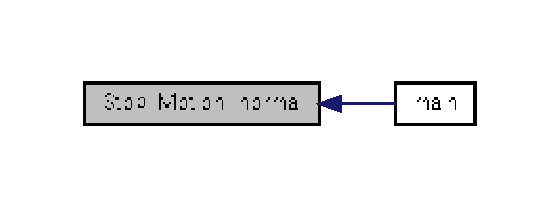
\includegraphics[width=268pt]{group__biba__drv_ga95c2965416e69e644b9f5a482707ae9f_icgraph}
\end{center}
\end{figure}


\hypertarget{group__biba__drv_gaaefaac2ed4c54f2008d8d236392c7261}{\index{D\-R\-V8825 Library@{D\-R\-V8825 Library}!store@{store}}
\index{store@{store}!DRV8825 Library@{D\-R\-V8825 Library}}
\subsubsection[{store}]{\setlength{\rightskip}{0pt plus 5cm}void store (
\begin{DoxyParamCaption}
\item[{void}]{}
\end{DoxyParamCaption}
)}}\label{group__biba__drv_gaaefaac2ed4c54f2008d8d236392c7261}
Calculates the real maximum speed,real minimum speed, real acceleration, steps per revolution, current mode and the current decay. \begin{DoxyReturn}{Returns}
void 
\end{DoxyReturn}


Definition at line 820 of file drv\-\_\-8825.\-c.


\begin{DoxyCode}
821 \{
822     eeprom\_write\_word( ( uint16\_t * ) ( 0 ), \hyperlink{drv__8825_8c_a2e720ed1ed0ef90dba27c1f246048dcd}{RealSpeed}.\hyperlink{structMotor__Parameters_a501458e333945f49f03c295e2f49e3b9}{MaxSpeed} );
823     eeprom\_write\_word( ( uint16\_t * ) ( 2 ), \hyperlink{drv__8825_8c_a2e720ed1ed0ef90dba27c1f246048dcd}{RealSpeed}.\hyperlink{structMotor__Parameters_aaf0ac3ed818f5c89cc86ea1d9174dc43}{MinSpeed} );
824     eeprom\_write\_word( ( uint16\_t * ) ( 4 ), \hyperlink{drv__8825_8c_a2e720ed1ed0ef90dba27c1f246048dcd}{RealSpeed}.\hyperlink{structMotor__Parameters_aa9f1146edc6d945d535eec80a01481f1}{Acceleration} );
825     eeprom\_write\_word( ( uint16\_t * ) ( 6 ), \hyperlink{drv__8825_8c_a54128bfe0cfae9cbd8577cf456951f21}{StepsPerRev} );
826     eeprom\_write\_byte( ( uint8\_t * ) ( 8 ), \hyperlink{drv__8825_8c_ab08e51d202664c8cc9434eac6c46f1f3}{CurrentMode} );
827     eeprom\_write\_byte( ( uint8\_t * ) ( 9 ), \hyperlink{drv__8825_8c_a1cc7e950196402ba79f3e5098b08fa33}{CurrentDecay} );
828 
829 
830 \}
\end{DoxyCode}


Here is the caller graph for this function\-:
\nopagebreak
\begin{figure}[H]
\begin{center}
\leavevmode
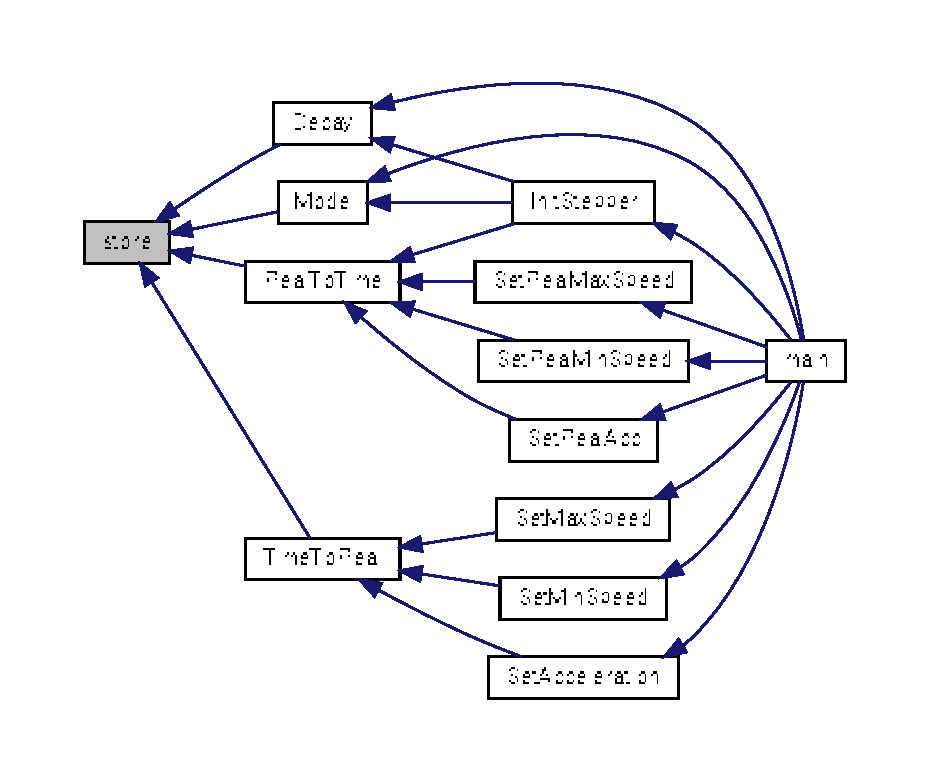
\includegraphics[width=350pt]{group__biba__drv_gaaefaac2ed4c54f2008d8d236392c7261_icgraph}
\end{center}
\end{figure}


\hypertarget{group__biba__drv_gaec239a01fef85140bc7c12fa612f421b}{\index{D\-R\-V8825 Library@{D\-R\-V8825 Library}!Time\-To\-Real@{Time\-To\-Real}}
\index{Time\-To\-Real@{Time\-To\-Real}!DRV8825 Library@{D\-R\-V8825 Library}}
\subsubsection[{Time\-To\-Real}]{\setlength{\rightskip}{0pt plus 5cm}void Time\-To\-Real (
\begin{DoxyParamCaption}
\item[{void}]{}
\end{DoxyParamCaption}
)}}\label{group__biba__drv_gaec239a01fef85140bc7c12fa612f421b}
Calculates the timmer speed to the real speed. \begin{DoxyReturn}{Returns}
void 
\end{DoxyReturn}


Definition at line 652 of file drv\-\_\-8825.\-c.


\begin{DoxyCode}
653 \{
654     uint16\_t r;
655     \hyperlink{drv__8825_8c_a2e720ed1ed0ef90dba27c1f246048dcd}{RealSpeed}.\hyperlink{structMotor__Parameters_a501458e333945f49f03c295e2f49e3b9}{MaxSpeed}=\hyperlink{group__biba__drv_gabc1e78364b977fdff7ae3b642e720f58}{HelperTtoR}(\hyperlink{drv__8825_8c_a7d20b8cec6f96108790d4bf76b9c469d}{TimeParam}.
      \hyperlink{structMotor__Parameters_a501458e333945f49f03c295e2f49e3b9}{MaxSpeed});
656     \hyperlink{drv__8825_8c_a2e720ed1ed0ef90dba27c1f246048dcd}{RealSpeed}.\hyperlink{structMotor__Parameters_aaf0ac3ed818f5c89cc86ea1d9174dc43}{MinSpeed}=\hyperlink{group__biba__drv_gabc1e78364b977fdff7ae3b642e720f58}{HelperTtoR}(\hyperlink{drv__8825_8c_a7d20b8cec6f96108790d4bf76b9c469d}{TimeParam}.
      \hyperlink{structMotor__Parameters_aaf0ac3ed818f5c89cc86ea1d9174dc43}{MinSpeed});
657 
658 \textcolor{comment}{/*}
659 \textcolor{comment}{    }
660 \textcolor{comment}{}
661 \textcolor{comment}{    //const uint64\_t l=1000000000*60;}
662 \textcolor{comment}{}
663 \textcolor{comment}{    r = TimeParam.MaxSpeed;}
664 \textcolor{comment}{}
665 \textcolor{comment}{    r = r * PERTMR;}
666 \textcolor{comment}{    r = r*StepsPerRev;}
667 \textcolor{comment}{    r = 10000000000 / r;}
668 \textcolor{comment}{    r = r * 6;}
669 \textcolor{comment}{}
670 \textcolor{comment}{}
671 \textcolor{comment}{}
672 \textcolor{comment}{}
673 \textcolor{comment}{    if ( r > 1 )}
674 \textcolor{comment}{    \{}
675 \textcolor{comment}{        RealSpeed.MaxSpeed = r;}
676 \textcolor{comment}{    \} else}
677 \textcolor{comment}{    \{}
678 \textcolor{comment}{        RealSpeed.MaxSpeed = 1;}
679 \textcolor{comment}{        //putstring\_P( PSTR( "Target MaxSpeed\(\backslash\)r" ) );}
680 \textcolor{comment}{    \}}
681 \textcolor{comment}{}
682 \textcolor{comment}{}
683 \textcolor{comment}{    r = TimeParam.MinSpeed;}
684 \textcolor{comment}{    r = r * PERTMR;}
685 \textcolor{comment}{    r = r*StepsPerRev;}
686 \textcolor{comment}{    r = 60000000000 / r;}
687 \textcolor{comment}{    //r=r*6;}
688 \textcolor{comment}{}
689 \textcolor{comment}{}
690 \textcolor{comment}{    if ( r > 1 )}
691 \textcolor{comment}{    \{}
692 \textcolor{comment}{        RealSpeed.MinSpeed = r;}
693 \textcolor{comment}{    \} else}
694 \textcolor{comment}{    \{}
695 \textcolor{comment}{        RealSpeed.MinSpeed = 1;}
696 \textcolor{comment}{        //putstring\_P( PSTR( "Target Minspeed\(\backslash\)r" ) );}
697 \textcolor{comment}{    \}}
698 \textcolor{comment}{}
699 \textcolor{comment}{*/}
700 
701     r = ( \hyperlink{drv__8825_8c_a7d20b8cec6f96108790d4bf76b9c469d}{TimeParam}.\hyperlink{structMotor__Parameters_aaf0ac3ed818f5c89cc86ea1d9174dc43}{MinSpeed} - \hyperlink{drv__8825_8c_a7d20b8cec6f96108790d4bf76b9c469d}{TimeParam}.\hyperlink{structMotor__Parameters_a501458e333945f49f03c295e2f49e3b9}{MaxSpeed} ) / 
      \hyperlink{drv__8825_8c_a7d20b8cec6f96108790d4bf76b9c469d}{TimeParam}.\hyperlink{structMotor__Parameters_aa9f1146edc6d945d535eec80a01481f1}{Acceleration};
702 
703     if ( r < 1 )
704     \{
705         \hyperlink{drv__8825_8c_a2e720ed1ed0ef90dba27c1f246048dcd}{RealSpeed}.\hyperlink{structMotor__Parameters_aa9f1146edc6d945d535eec80a01481f1}{Acceleration} = 1;
706         \textcolor{comment}{//putstring\_P( PSTR( "Acc low\(\backslash\)r" ) );}
707     \} \textcolor{keywordflow}{else}
708     \{
709         \hyperlink{drv__8825_8c_a2e720ed1ed0ef90dba27c1f246048dcd}{RealSpeed}.\hyperlink{structMotor__Parameters_aa9f1146edc6d945d535eec80a01481f1}{Acceleration} = r;
710     \}
711 
712     \hyperlink{group__biba__drv_ga3389079a7106f1e741c0bc447dfbcbca}{CalWorkParam}( );
713     \hyperlink{group__biba__drv_gaaefaac2ed4c54f2008d8d236392c7261}{store}( );
714 \}
\end{DoxyCode}


Here is the call graph for this function\-:
\nopagebreak
\begin{figure}[H]
\begin{center}
\leavevmode
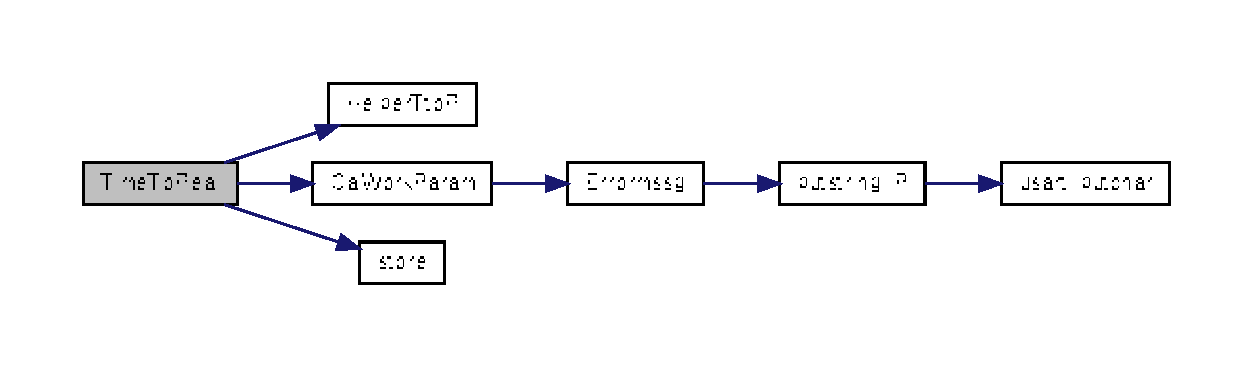
\includegraphics[width=350pt]{group__biba__drv_gaec239a01fef85140bc7c12fa612f421b_cgraph}
\end{center}
\end{figure}




Here is the caller graph for this function\-:
\nopagebreak
\begin{figure}[H]
\begin{center}
\leavevmode
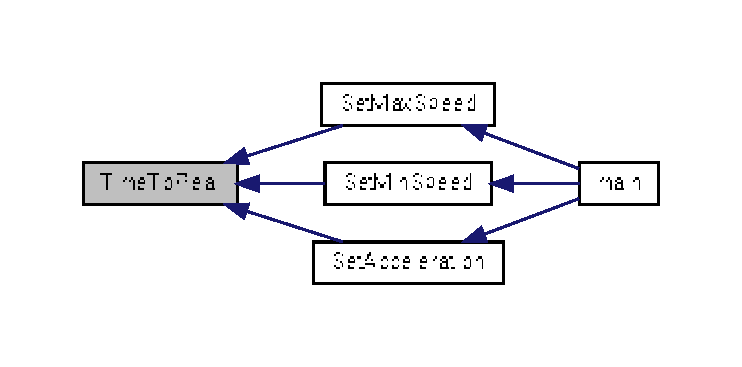
\includegraphics[width=350pt]{group__biba__drv_gaec239a01fef85140bc7c12fa612f421b_icgraph}
\end{center}
\end{figure}


\hypertarget{group__biba__drv_ga102f936b773a4a26032cc6b8cd1a273d}{\index{D\-R\-V8825 Library@{D\-R\-V8825 Library}!Way\-\_\-\-Speed@{Way\-\_\-\-Speed}}
\index{Way\-\_\-\-Speed@{Way\-\_\-\-Speed}!DRV8825 Library@{D\-R\-V8825 Library}}
\subsubsection[{Way\-\_\-\-Speed}]{\setlength{\rightskip}{0pt plus 5cm}void Way\-\_\-\-Speed (
\begin{DoxyParamCaption}
\item[{{\bf step\-\_\-type}}]{step}
\end{DoxyParamCaption}
)}}\label{group__biba__drv_ga102f936b773a4a26032cc6b8cd1a273d}
Movement with constant speed and constant r\-P\-M \begin{DoxySeeAlso}{See Also}
\hyperlink{group__biba__drv_ga3af682b92aa259509aea217f6dc64356}{step\-\_\-type} 
\end{DoxySeeAlso}

\begin{DoxyParams}{Parameters}
{\em step} & the first argument. \\
\hline
\end{DoxyParams}
\begin{DoxyReturn}{Returns}
void 
\end{DoxyReturn}


Definition at line 339 of file drv\-\_\-8825.\-c.


\begin{DoxyCode}
340 \{
341     \hyperlink{drv__8825_8c_a295a33258d6c0cfd0dd62f0574952f21}{ConstSpd} = 1;
342     \hyperlink{group__biba__drv_ga961e1c89176d3c56101bb4eddf6642dc}{Count\_Step}( step, 60000 );
343 \}
\end{DoxyCode}


Here is the call graph for this function\-:
\nopagebreak
\begin{figure}[H]
\begin{center}
\leavevmode
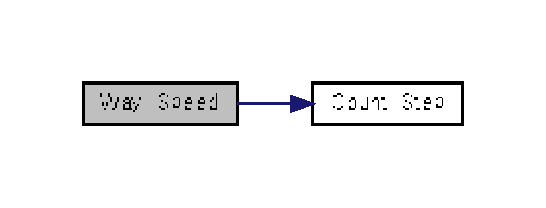
\includegraphics[width=262pt]{group__biba__drv_ga102f936b773a4a26032cc6b8cd1a273d_cgraph}
\end{center}
\end{figure}




Here is the caller graph for this function\-:
\nopagebreak
\begin{figure}[H]
\begin{center}
\leavevmode
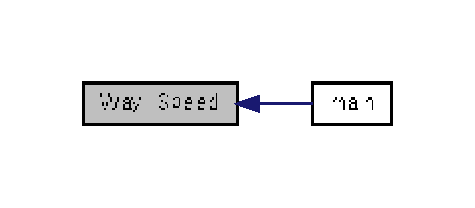
\includegraphics[width=228pt]{group__biba__drv_ga102f936b773a4a26032cc6b8cd1a273d_icgraph}
\end{center}
\end{figure}



\hypertarget{group__biba__main}{\section{main Library}
\label{group__biba__main}\index{main Library@{main Library}}
}


This turns on the motor and directly goes in the continuos loop for controlling it.  


\subsection*{Functions}
\begin{DoxyCompactItemize}
\item 
void \hyperlink{group__biba__main_ga18fa08105e4cb9cce10290e3c5c4ca01}{Init\-\_\-\-Input\-\_\-\-Output} (void)
\item 
void \hyperlink{group__biba__main_ga708a4c1a4d0c4acc4c447310dd4db27f}{test} (void)
\end{DoxyCompactItemize}


\subsection{Detailed Description}
This turns on the motor and directly goes in the continuos loop for controlling it. 
\begin{DoxyCode}
\textcolor{preprocessor}{#include <\hyperlink{main_8h}{main.h}>} 
\end{DoxyCode}


This turns on the motor and directly goes in the continuos loop for controlling it.

\begin{DoxyNote}{Note}
this is whear all the magic happens 
\end{DoxyNote}
\begin{DoxyAuthor}{Author}
Bilyana Borisova \href{mailto:bibishte@gmail.com}{\tt bibishte@gmail.\-com} 
\end{DoxyAuthor}


\subsection{Function Documentation}
\hypertarget{group__biba__main_ga18fa08105e4cb9cce10290e3c5c4ca01}{\index{main Library@{main Library}!Init\-\_\-\-Input\-\_\-\-Output@{Init\-\_\-\-Input\-\_\-\-Output}}
\index{Init\-\_\-\-Input\-\_\-\-Output@{Init\-\_\-\-Input\-\_\-\-Output}!main Library@{main Library}}
\subsubsection[{Init\-\_\-\-Input\-\_\-\-Output}]{\setlength{\rightskip}{0pt plus 5cm}void Init\-\_\-\-Input\-\_\-\-Output (
\begin{DoxyParamCaption}
\item[{void}]{}
\end{DoxyParamCaption}
)}}\label{group__biba__main_ga18fa08105e4cb9cce10290e3c5c4ca01}
Initial initialisation of input and output of microcontroller \begin{DoxyReturn}{Returns}
void 
\end{DoxyReturn}


Definition at line 561 of file main.\-c.


\begin{DoxyCode}
562 \{
563     \textcolor{comment}{//input init}
564 
565     \hyperlink{group__biba__config_gaf5147cefc7b56baad8c6337a315ce07f}{set\_as\_input}( \hyperlink{group__biba__config_ga90f5e4a0bd154d1e2b2a6f688dced82e}{DRXD}, \hyperlink{group__biba__config_ga95855eaf9cee62de5402f124b1b8a27b}{RXD} );
566     \hyperlink{group__biba__config_gaf5147cefc7b56baad8c6337a315ce07f}{set\_as\_input}( \hyperlink{group__biba__config_ga80ca054824bc462b54a3fcfdf7f6be87}{DHOME}, \hyperlink{group__biba__config_ga0e26ea2db1b570d1a6fe1ac180ef4541}{HOME} );
567     \hyperlink{group__biba__config_gaf5147cefc7b56baad8c6337a315ce07f}{set\_as\_input}( \hyperlink{group__biba__config_ga813e08916fb1e6f00505d36e1bb830c3}{DSCL}, \hyperlink{group__biba__config_gab5ffc4751921608954bb7a5687566b2d}{SCL} );
568     \hyperlink{group__biba__config_gaf5147cefc7b56baad8c6337a315ce07f}{set\_as\_input}( \hyperlink{group__biba__config_gafc00dbf97764b4d68c05e9bfc6761e4d}{DMISO}, \hyperlink{group__biba__config_ga7334c540878c8c4d801fd75ed9fd8063}{MISO} );
569     \hyperlink{group__biba__config_gaf5147cefc7b56baad8c6337a315ce07f}{set\_as\_input}( \hyperlink{group__biba__config_ga6b14a46014e8d8efa630e7df0f08b368}{DFAULT}, \hyperlink{group__biba__config_ga4115eb21750f37d540839cc51fca5401}{FAULT} );
570 
571     \hyperlink{group__biba__config_ga4ee07d04aa2ef10d631d61c17c558464}{set\_bit}( \hyperlink{group__biba__config_gae632439c6ad45e36bc003a03e22e9e7a}{PRXD}, \hyperlink{group__biba__config_ga95855eaf9cee62de5402f124b1b8a27b}{RXD} );
572     \hyperlink{group__biba__config_ga4ee07d04aa2ef10d631d61c17c558464}{set\_bit}( \hyperlink{group__biba__config_ga40b96047acab9312add35336b138f140}{PSCL}, \hyperlink{group__biba__config_gab5ffc4751921608954bb7a5687566b2d}{SCL} );
573     \hyperlink{group__biba__config_ga4ee07d04aa2ef10d631d61c17c558464}{set\_bit}( \hyperlink{group__biba__config_gaaf98ae1f6b0c231d734e204906a0e992}{PMISO}, \hyperlink{group__biba__config_ga7334c540878c8c4d801fd75ed9fd8063}{MISO} );
574     \hyperlink{group__biba__config_ga4ee07d04aa2ef10d631d61c17c558464}{set\_bit}(\hyperlink{group__biba__config_ga431ab20bf2b9e58830a8ecd2a294e8bc}{PHOME}, \hyperlink{group__biba__config_ga0e26ea2db1b570d1a6fe1ac180ef4541}{HOME});
575 
576     \textcolor{comment}{//output init}
577 
578     \hyperlink{group__biba__config_ga91fb0adcf6533b4acfe793396836badc}{set\_as\_output}( \hyperlink{group__biba__config_ga11a7f88811704d85bf9e6e88e5b4a13a}{DENABLE\_STEPPER}, \hyperlink{group__biba__config_gaf43f2237d47f7e2e48d74999befaa9fd}{ENABLE\_STEPPER} );
579     \hyperlink{group__biba__config_ga91fb0adcf6533b4acfe793396836badc}{set\_as\_output}( \hyperlink{group__biba__config_gafcb7b56ec9ef5d20fcc86f61034a6a73}{DTXD}, \hyperlink{group__biba__config_ga0466ccb605cb0395fb03b72f476ec855}{TXD} );
580     \hyperlink{group__biba__config_ga91fb0adcf6533b4acfe793396836badc}{set\_as\_output}( \hyperlink{group__biba__config_ga652846ae5576cfc7a97e79569c9b9426}{DMODE0}, \hyperlink{group__biba__config_ga5daa4b780b82b5e8678d8c7095336b62}{MODE0} );
581     \hyperlink{group__biba__config_ga91fb0adcf6533b4acfe793396836badc}{set\_as\_output}( \hyperlink{group__biba__config_ga583975602ab120ab85362c7281e4b1dc}{DMODE1}, \hyperlink{group__biba__config_ga443b1268c43b309560d57e34d50b5b3b}{MODE1} );
582     \hyperlink{group__biba__config_ga91fb0adcf6533b4acfe793396836badc}{set\_as\_output}( \hyperlink{group__biba__config_gab30b2507134f18696809327fcfb86c51}{DMODE2}, \hyperlink{group__biba__config_gab2d8aca64e351712eae6f03e3f9d64ad}{MODE2} );
583     \hyperlink{group__biba__config_gaf5147cefc7b56baad8c6337a315ce07f}{set\_as\_input}( \hyperlink{group__biba__config_ga4280725e4eff1145eac3e34c574b8383}{DDECAY}, \hyperlink{group__biba__config_ga9d211c41bcae2aa62028a3645c63cf8a}{DECAY} );
584     \hyperlink{group__biba__config_ga91fb0adcf6533b4acfe793396836badc}{set\_as\_output}( \hyperlink{group__biba__config_gafec4ba65dc31b3c5c4ca6a3471054994}{DSTEP}, \hyperlink{group__biba__config_ga70be2dc5c8bdc85b027ea6118753cca1}{STEP} );
585     \hyperlink{group__biba__config_ga91fb0adcf6533b4acfe793396836badc}{set\_as\_output}( \hyperlink{group__biba__config_ga1421c0c377bbe274867c9dbaca51d707}{DMOSI}, \hyperlink{group__biba__config_ga5d3f11f2fdf8a7e27b975291e0c2c8cc}{MOSI} );
586     \hyperlink{group__biba__config_ga91fb0adcf6533b4acfe793396836badc}{set\_as\_output}( \hyperlink{group__biba__config_ga75cfe7b50065d13aa41a1b28815b78df}{DDIRECTION}, \hyperlink{group__biba__config_ga1d692daf1ffadae2243a5ab556589629}{DIRECTION} );
587     \hyperlink{group__biba__config_ga91fb0adcf6533b4acfe793396836badc}{set\_as\_output}( \hyperlink{group__biba__config_gab2a611474dce8378023836a4c5e07b3a}{DDIR\_485}, \hyperlink{group__biba__config_ga251b49d43197436ec9943946734a7945}{DIR\_485} );
588 
589     \hyperlink{group__biba__config_ga4ee07d04aa2ef10d631d61c17c558464}{set\_bit}( \hyperlink{group__biba__config_gaf49566bede8af55a9c7c7cb49722ca8a}{PENABLE\_STEPPER}, \hyperlink{group__biba__config_gaf43f2237d47f7e2e48d74999befaa9fd}{ENABLE\_STEPPER} );
590     \hyperlink{group__biba__config_gaf2f231c38a29a96bac24f174fe7bf8b0}{clr\_bit}( \hyperlink{group__biba__config_gac31c37de4ad57d7e8e88d6a4ceb1a526}{PMODE0}, \hyperlink{group__biba__config_ga5daa4b780b82b5e8678d8c7095336b62}{MODE0} );
591     \hyperlink{group__biba__config_gaf2f231c38a29a96bac24f174fe7bf8b0}{clr\_bit}( \hyperlink{group__biba__config_gae2b3b81d452af91ecd26298a6a9954a8}{PMODE1}, \hyperlink{group__biba__config_ga443b1268c43b309560d57e34d50b5b3b}{MODE1} );
592     \hyperlink{group__biba__config_gaf2f231c38a29a96bac24f174fe7bf8b0}{clr\_bit}( \hyperlink{group__biba__config_ga4e6fd56609bbd34dc3797ee35d8610e8}{PMODE2}, \hyperlink{group__biba__config_gab2d8aca64e351712eae6f03e3f9d64ad}{MODE2} );
593     \hyperlink{group__biba__config_gaf2f231c38a29a96bac24f174fe7bf8b0}{clr\_bit}( \hyperlink{group__biba__config_ga42a58bd5ca7d52e02b78dbc498bd18fc}{PDECAY}, \hyperlink{group__biba__config_ga9d211c41bcae2aa62028a3645c63cf8a}{DECAY} );
594     \hyperlink{group__biba__config_gaf2f231c38a29a96bac24f174fe7bf8b0}{clr\_bit}( \hyperlink{group__biba__config_ga27c908eae571c75c5a5e37d6fcc8db9d}{PDIRECTION}, \hyperlink{group__biba__config_ga1d692daf1ffadae2243a5ab556589629}{DIRECTION} );
595     \hyperlink{group__biba__config_ga4ee07d04aa2ef10d631d61c17c558464}{set\_bit}( \hyperlink{group__biba__config_ga68d026b2f91c535d306bc10e7576056f}{PDIR\_485}, \hyperlink{group__biba__config_ga251b49d43197436ec9943946734a7945}{DIR\_485} );
596 
597 \}
\end{DoxyCode}


Here is the caller graph for this function\-:
\nopagebreak
\begin{figure}[H]
\begin{center}
\leavevmode
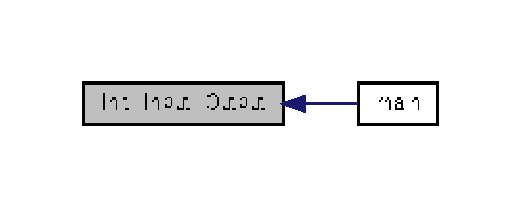
\includegraphics[width=250pt]{group__biba__main_ga18fa08105e4cb9cce10290e3c5c4ca01_icgraph}
\end{center}
\end{figure}


\hypertarget{group__biba__main_ga708a4c1a4d0c4acc4c447310dd4db27f}{\index{main Library@{main Library}!test@{test}}
\index{test@{test}!main Library@{main Library}}
\subsubsection[{test}]{\setlength{\rightskip}{0pt plus 5cm}void test (
\begin{DoxyParamCaption}
\item[{void}]{}
\end{DoxyParamCaption}
)}}\label{group__biba__main_ga708a4c1a4d0c4acc4c447310dd4db27f}
Just for testing \begin{DoxyReturn}{Returns}
void 
\end{DoxyReturn}


Definition at line 603 of file main.\-c.


\begin{DoxyCode}
604 \{
605     \hyperlink{group__biba__utils_gaf1b54c4c5b890362b485636395859b3d}{putstring\_P}( PSTR( \textcolor{stringliteral}{"Test?"} ) );
606 
607 \}
\end{DoxyCode}


Here is the call graph for this function\-:
\nopagebreak
\begin{figure}[H]
\begin{center}
\leavevmode
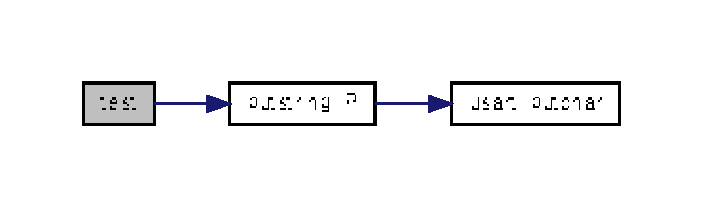
\includegraphics[width=338pt]{group__biba__main_ga708a4c1a4d0c4acc4c447310dd4db27f_cgraph}
\end{center}
\end{figure}




Here is the caller graph for this function\-:
\nopagebreak
\begin{figure}[H]
\begin{center}
\leavevmode
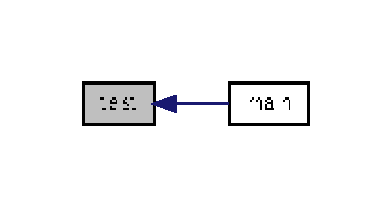
\includegraphics[width=188pt]{group__biba__main_ga708a4c1a4d0c4acc4c447310dd4db27f_icgraph}
\end{center}
\end{figure}



\hypertarget{group__biba__messges}{\section{messages Library}
\label{group__biba__messges}\index{messages Library@{messages Library}}
}


This module contains functions that are printing messages.  


\subsection*{Functions}
\begin{DoxyCompactItemize}
\item 
void \hyperlink{group__biba__messges_ga6e96dc2b209da9d4eef98fb809f1f615}{Acc} (void)
\item 
void \hyperlink{group__biba__messges_ga4df90f192fc647ecf71806dc05b290b5}{A\-Dec} (void)
\item 
void \hyperlink{group__biba__messges_gaa77012dc6d2b6aba302311b04e512abc}{Errormssg} (void)
\item 
void \hyperlink{group__biba__messges_ga0dd076c947adc7f37ed9024c16def436}{F\-Dec} (void)
\item 
void \hyperlink{group__biba__messges_ga6a0297ad8db89b689f7314473dd7cd7a}{Fstep} (void)
\item 
void \hyperlink{group__biba__messges_ga53669298f54817f8d2b140050dc910f1}{H\-Step} (void)
\item 
void \hyperlink{group__biba__messges_ga286e4f6b6038548b06d71fb6badfd28b}{M16\-Step} (void)
\item 
void \hyperlink{group__biba__messges_ga5b419cf59d479fba5c67c575b553e158}{M32\-Step} (void)
\item 
void \hyperlink{group__biba__messges_ga40b8844aa998b3549f6194d437100ee7}{M8\-Step} (void)
\item 
void \hyperlink{group__biba__messges_gaa5f13f30a59a97aca9198b06a0c90112}{Maxspeed} (void)
\item 
void \hyperlink{group__biba__messges_ga46822b53dd41e304ef1887ef7075ffd7}{Minspeed} (void)
\item 
void \hyperlink{group__biba__messges_ga11901ed666ca738e518ff569cf8d947a}{Qstep} (void)
\item 
void \hyperlink{group__biba__messges_gad576f94f72a14d6cf14d7a3217d3fdb5}{R\-Acc} (void)
\item 
void \hyperlink{group__biba__messges_ga1cee417b557775a8a769eb5bc2306f08}{R\-Max\-Spd} (void)
\item 
void \hyperlink{group__biba__messges_gaabc2b68cf794e6851e1826ba9e083c3b}{R\-Min\-Spd} (void)
\item 
void \hyperlink{group__biba__messges_gad5028f9e871f7e63759218b94a829f45}{S\-Dec} (void)
\item 
void \hyperlink{group__biba__messges_ga98ca8e64d40da656ab802f68b0eb84a1}{Spt\-Revol} (void)
\item 
void \hyperlink{group__biba__messges_ga76c658dc5f4332e4b034419dca518c1c}{Stop} (void)
\end{DoxyCompactItemize}


\subsection{Detailed Description}
This module contains functions that are printing messages. 
\begin{DoxyCode}
\textcolor{preprocessor}{#include <\hyperlink{messages_8h}{messages.h}>} 
\end{DoxyCode}


This module contains functions that are printing stuff

\begin{DoxyNote}{Note}
Typical functions that are saving me memory. 
\end{DoxyNote}
\begin{DoxyAuthor}{Author}
Bilyana Borisova \href{mailto:bibishte@gmail.com}{\tt bibishte@gmail.\-com} 
\end{DoxyAuthor}


\subsection{Function Documentation}
\hypertarget{group__biba__messges_ga6e96dc2b209da9d4eef98fb809f1f615}{\index{messages Library@{messages Library}!Acc@{Acc}}
\index{Acc@{Acc}!messages Library@{messages Library}}
\subsubsection[{Acc}]{\setlength{\rightskip}{0pt plus 5cm}void Acc (
\begin{DoxyParamCaption}
\item[{void}]{}
\end{DoxyParamCaption}
)}}\label{group__biba__messges_ga6e96dc2b209da9d4eef98fb809f1f615}


Definition at line 77 of file messages.\-c.


\begin{DoxyCode}
78 \{
79     \hyperlink{group__biba__utils_gaf1b54c4c5b890362b485636395859b3d}{putstring\_P}( PSTR( \textcolor{stringliteral}{"Acc="} ) );
80     \hyperlink{group__biba__utils_ga354be7728c1265a82ba2510f1800cea4}{putstring}( \hyperlink{group__biba__utils_ga3d33c2ff89043a4bf00d652d182dfc27}{int\_to\_string}( ( uint64\_t ) ( 
      \hyperlink{group__biba__drv_ga6202c4fd41a45376809e5940428467b9}{GetAcceleration}( ) ) ) );
81     \hyperlink{group__biba__utils_gaf1b54c4c5b890362b485636395859b3d}{putstring\_P}( PSTR( \textcolor{stringliteral}{"\(\backslash\)r"} ) );
82 \}
\end{DoxyCode}


Here is the call graph for this function\-:
\nopagebreak
\begin{figure}[H]
\begin{center}
\leavevmode
\includegraphics[width=350pt]{group__biba__messges_ga6e96dc2b209da9d4eef98fb809f1f615_cgraph}
\end{center}
\end{figure}




Here is the caller graph for this function\-:
\nopagebreak
\begin{figure}[H]
\begin{center}
\leavevmode
\includegraphics[width=188pt]{group__biba__messges_ga6e96dc2b209da9d4eef98fb809f1f615_icgraph}
\end{center}
\end{figure}


\hypertarget{group__biba__messges_ga4df90f192fc647ecf71806dc05b290b5}{\index{messages Library@{messages Library}!A\-Dec@{A\-Dec}}
\index{A\-Dec@{A\-Dec}!messages Library@{messages Library}}
\subsubsection[{A\-Dec}]{\setlength{\rightskip}{0pt plus 5cm}void A\-Dec (
\begin{DoxyParamCaption}
\item[{void}]{}
\end{DoxyParamCaption}
)}}\label{group__biba__messges_ga4df90f192fc647ecf71806dc05b290b5}


Definition at line 42 of file messages.\-c.


\begin{DoxyCode}
43 \{
44     \hyperlink{group__biba__utils_gaf1b54c4c5b890362b485636395859b3d}{putstring\_P}( PSTR( \textcolor{stringliteral}{"ADec\(\backslash\)r"} ) );
45 \}
\end{DoxyCode}


Here is the call graph for this function\-:
\nopagebreak
\begin{figure}[H]
\begin{center}
\leavevmode
\includegraphics[width=346pt]{group__biba__messges_ga4df90f192fc647ecf71806dc05b290b5_cgraph}
\end{center}
\end{figure}




Here is the caller graph for this function\-:
\nopagebreak
\begin{figure}[H]
\begin{center}
\leavevmode
\includegraphics[width=196pt]{group__biba__messges_ga4df90f192fc647ecf71806dc05b290b5_icgraph}
\end{center}
\end{figure}


\hypertarget{group__biba__messges_gaa77012dc6d2b6aba302311b04e512abc}{\index{messages Library@{messages Library}!Errormssg@{Errormssg}}
\index{Errormssg@{Errormssg}!messages Library@{messages Library}}
\subsubsection[{Errormssg}]{\setlength{\rightskip}{0pt plus 5cm}void Errormssg (
\begin{DoxyParamCaption}
\item[{void}]{}
\end{DoxyParamCaption}
)}}\label{group__biba__messges_gaa77012dc6d2b6aba302311b04e512abc}


Definition at line 91 of file messages.\-c.


\begin{DoxyCode}
92 \{
93     \hyperlink{group__biba__utils_gaf1b54c4c5b890362b485636395859b3d}{putstring\_P}( PSTR( \textcolor{stringliteral}{"ERROR\(\backslash\)r"} ) );
94 \}
\end{DoxyCode}


Here is the call graph for this function\-:
\nopagebreak
\begin{figure}[H]
\begin{center}
\leavevmode
\includegraphics[width=350pt]{group__biba__messges_gaa77012dc6d2b6aba302311b04e512abc_cgraph}
\end{center}
\end{figure}




Here is the caller graph for this function\-:
\nopagebreak
\begin{figure}[H]
\begin{center}
\leavevmode
\includegraphics[width=350pt]{group__biba__messges_gaa77012dc6d2b6aba302311b04e512abc_icgraph}
\end{center}
\end{figure}


\hypertarget{group__biba__messges_ga0dd076c947adc7f37ed9024c16def436}{\index{messages Library@{messages Library}!F\-Dec@{F\-Dec}}
\index{F\-Dec@{F\-Dec}!messages Library@{messages Library}}
\subsubsection[{F\-Dec}]{\setlength{\rightskip}{0pt plus 5cm}void F\-Dec (
\begin{DoxyParamCaption}
\item[{void}]{}
\end{DoxyParamCaption}
)}}\label{group__biba__messges_ga0dd076c947adc7f37ed9024c16def436}


Definition at line 37 of file messages.\-c.


\begin{DoxyCode}
38 \{
39     \hyperlink{group__biba__utils_gaf1b54c4c5b890362b485636395859b3d}{putstring\_P}( PSTR( \textcolor{stringliteral}{"FDec\(\backslash\)r"} ) );
40 \}
\end{DoxyCode}


Here is the call graph for this function\-:
\nopagebreak
\begin{figure}[H]
\begin{center}
\leavevmode
\includegraphics[width=346pt]{group__biba__messges_ga0dd076c947adc7f37ed9024c16def436_cgraph}
\end{center}
\end{figure}




Here is the caller graph for this function\-:
\nopagebreak
\begin{figure}[H]
\begin{center}
\leavevmode
\includegraphics[width=196pt]{group__biba__messges_ga0dd076c947adc7f37ed9024c16def436_icgraph}
\end{center}
\end{figure}


\hypertarget{group__biba__messges_ga6a0297ad8db89b689f7314473dd7cd7a}{\index{messages Library@{messages Library}!Fstep@{Fstep}}
\index{Fstep@{Fstep}!messages Library@{messages Library}}
\subsubsection[{Fstep}]{\setlength{\rightskip}{0pt plus 5cm}void Fstep (
\begin{DoxyParamCaption}
\item[{void}]{}
\end{DoxyParamCaption}
)}}\label{group__biba__messges_ga6a0297ad8db89b689f7314473dd7cd7a}


Definition at line 47 of file messages.\-c.


\begin{DoxyCode}
48 \{
49     \hyperlink{group__biba__utils_gaf1b54c4c5b890362b485636395859b3d}{putstring\_P}( PSTR( \textcolor{stringliteral}{"full step\(\backslash\)r"} ) );
50 \}
\end{DoxyCode}


Here is the call graph for this function\-:
\nopagebreak
\begin{figure}[H]
\begin{center}
\leavevmode
\includegraphics[width=348pt]{group__biba__messges_ga6a0297ad8db89b689f7314473dd7cd7a_cgraph}
\end{center}
\end{figure}




Here is the caller graph for this function\-:
\nopagebreak
\begin{figure}[H]
\begin{center}
\leavevmode
\includegraphics[width=198pt]{group__biba__messges_ga6a0297ad8db89b689f7314473dd7cd7a_icgraph}
\end{center}
\end{figure}


\hypertarget{group__biba__messges_ga53669298f54817f8d2b140050dc910f1}{\index{messages Library@{messages Library}!H\-Step@{H\-Step}}
\index{H\-Step@{H\-Step}!messages Library@{messages Library}}
\subsubsection[{H\-Step}]{\setlength{\rightskip}{0pt plus 5cm}void H\-Step (
\begin{DoxyParamCaption}
\item[{void}]{}
\end{DoxyParamCaption}
)}}\label{group__biba__messges_ga53669298f54817f8d2b140050dc910f1}


Definition at line 52 of file messages.\-c.


\begin{DoxyCode}
53 \{
54     \hyperlink{group__biba__utils_gaf1b54c4c5b890362b485636395859b3d}{putstring\_P}( PSTR( \textcolor{stringliteral}{"half step\(\backslash\)r"} ) );
55 \}
\end{DoxyCode}


Here is the call graph for this function\-:
\nopagebreak
\begin{figure}[H]
\begin{center}
\leavevmode
\includegraphics[width=350pt]{group__biba__messges_ga53669298f54817f8d2b140050dc910f1_cgraph}
\end{center}
\end{figure}




Here is the caller graph for this function\-:
\nopagebreak
\begin{figure}[H]
\begin{center}
\leavevmode
\includegraphics[width=200pt]{group__biba__messges_ga53669298f54817f8d2b140050dc910f1_icgraph}
\end{center}
\end{figure}


\hypertarget{group__biba__messges_ga286e4f6b6038548b06d71fb6badfd28b}{\index{messages Library@{messages Library}!M16\-Step@{M16\-Step}}
\index{M16\-Step@{M16\-Step}!messages Library@{messages Library}}
\subsubsection[{M16\-Step}]{\setlength{\rightskip}{0pt plus 5cm}void M16\-Step (
\begin{DoxyParamCaption}
\item[{void}]{}
\end{DoxyParamCaption}
)}}\label{group__biba__messges_ga286e4f6b6038548b06d71fb6badfd28b}


Definition at line 67 of file messages.\-c.


\begin{DoxyCode}
68 \{
69     \hyperlink{group__biba__utils_gaf1b54c4c5b890362b485636395859b3d}{putstring\_P}( PSTR( \textcolor{stringliteral}{"16 microsteps\(\backslash\)r"} ) );
70 \}
\end{DoxyCode}


Here is the call graph for this function\-:
\nopagebreak
\begin{figure}[H]
\begin{center}
\leavevmode
\includegraphics[width=350pt]{group__biba__messges_ga286e4f6b6038548b06d71fb6badfd28b_cgraph}
\end{center}
\end{figure}




Here is the caller graph for this function\-:
\nopagebreak
\begin{figure}[H]
\begin{center}
\leavevmode
\includegraphics[width=214pt]{group__biba__messges_ga286e4f6b6038548b06d71fb6badfd28b_icgraph}
\end{center}
\end{figure}


\hypertarget{group__biba__messges_ga5b419cf59d479fba5c67c575b553e158}{\index{messages Library@{messages Library}!M32\-Step@{M32\-Step}}
\index{M32\-Step@{M32\-Step}!messages Library@{messages Library}}
\subsubsection[{M32\-Step}]{\setlength{\rightskip}{0pt plus 5cm}void M32\-Step (
\begin{DoxyParamCaption}
\item[{void}]{}
\end{DoxyParamCaption}
)}}\label{group__biba__messges_ga5b419cf59d479fba5c67c575b553e158}


Definition at line 72 of file messages.\-c.


\begin{DoxyCode}
73 \{
74     \hyperlink{group__biba__utils_gaf1b54c4c5b890362b485636395859b3d}{putstring\_P}( PSTR( \textcolor{stringliteral}{"32 microsteps\(\backslash\)r"} ) );
75 \}
\end{DoxyCode}


Here is the call graph for this function\-:
\nopagebreak
\begin{figure}[H]
\begin{center}
\leavevmode
\includegraphics[width=350pt]{group__biba__messges_ga5b419cf59d479fba5c67c575b553e158_cgraph}
\end{center}
\end{figure}




Here is the caller graph for this function\-:
\nopagebreak
\begin{figure}[H]
\begin{center}
\leavevmode
\includegraphics[width=214pt]{group__biba__messges_ga5b419cf59d479fba5c67c575b553e158_icgraph}
\end{center}
\end{figure}


\hypertarget{group__biba__messges_ga40b8844aa998b3549f6194d437100ee7}{\index{messages Library@{messages Library}!M8\-Step@{M8\-Step}}
\index{M8\-Step@{M8\-Step}!messages Library@{messages Library}}
\subsubsection[{M8\-Step}]{\setlength{\rightskip}{0pt plus 5cm}void M8\-Step (
\begin{DoxyParamCaption}
\item[{void}]{}
\end{DoxyParamCaption}
)}}\label{group__biba__messges_ga40b8844aa998b3549f6194d437100ee7}


Definition at line 62 of file messages.\-c.


\begin{DoxyCode}
63 \{
64     \hyperlink{group__biba__utils_gaf1b54c4c5b890362b485636395859b3d}{putstring\_P}( PSTR( \textcolor{stringliteral}{"8 microsteps\(\backslash\)r"} ) );
65 \}
\end{DoxyCode}


Here is the call graph for this function\-:
\nopagebreak
\begin{figure}[H]
\begin{center}
\leavevmode
\includegraphics[width=350pt]{group__biba__messges_ga40b8844aa998b3549f6194d437100ee7_cgraph}
\end{center}
\end{figure}




Here is the caller graph for this function\-:
\nopagebreak
\begin{figure}[H]
\begin{center}
\leavevmode
\includegraphics[width=208pt]{group__biba__messges_ga40b8844aa998b3549f6194d437100ee7_icgraph}
\end{center}
\end{figure}


\hypertarget{group__biba__messges_gaa5f13f30a59a97aca9198b06a0c90112}{\index{messages Library@{messages Library}!Maxspeed@{Maxspeed}}
\index{Maxspeed@{Maxspeed}!messages Library@{messages Library}}
\subsubsection[{Maxspeed}]{\setlength{\rightskip}{0pt plus 5cm}void Maxspeed (
\begin{DoxyParamCaption}
\item[{void}]{}
\end{DoxyParamCaption}
)}}\label{group__biba__messges_gaa5f13f30a59a97aca9198b06a0c90112}


Definition at line 96 of file messages.\-c.


\begin{DoxyCode}
97 \{
98     \hyperlink{group__biba__utils_gaf1b54c4c5b890362b485636395859b3d}{putstring\_P}( PSTR( \textcolor{stringliteral}{"MaxSPD="} ) );
99     \hyperlink{group__biba__utils_ga354be7728c1265a82ba2510f1800cea4}{putstring}( \hyperlink{group__biba__utils_ga3d33c2ff89043a4bf00d652d182dfc27}{int\_to\_string}( ( uint64\_t ) ( \hyperlink{group__biba__drv_ga356f958c8327643ae22d240493ae7747}{GetMaxSpeed}( ) ) ) );
100     \hyperlink{group__biba__utils_gaf1b54c4c5b890362b485636395859b3d}{putstring\_P}( PSTR( \textcolor{stringliteral}{"\(\backslash\)r"} ) );
101 \}
\end{DoxyCode}


Here is the call graph for this function\-:
\nopagebreak
\begin{figure}[H]
\begin{center}
\leavevmode
\includegraphics[width=350pt]{group__biba__messges_gaa5f13f30a59a97aca9198b06a0c90112_cgraph}
\end{center}
\end{figure}




Here is the caller graph for this function\-:
\nopagebreak
\begin{figure}[H]
\begin{center}
\leavevmode
\includegraphics[width=220pt]{group__biba__messges_gaa5f13f30a59a97aca9198b06a0c90112_icgraph}
\end{center}
\end{figure}


\hypertarget{group__biba__messges_ga46822b53dd41e304ef1887ef7075ffd7}{\index{messages Library@{messages Library}!Minspeed@{Minspeed}}
\index{Minspeed@{Minspeed}!messages Library@{messages Library}}
\subsubsection[{Minspeed}]{\setlength{\rightskip}{0pt plus 5cm}void Minspeed (
\begin{DoxyParamCaption}
\item[{void}]{}
\end{DoxyParamCaption}
)}}\label{group__biba__messges_ga46822b53dd41e304ef1887ef7075ffd7}


Definition at line 84 of file messages.\-c.


\begin{DoxyCode}
85 \{
86     \hyperlink{group__biba__utils_gaf1b54c4c5b890362b485636395859b3d}{putstring\_P}( PSTR( \textcolor{stringliteral}{"MinSPD="} ) );
87     \hyperlink{group__biba__utils_ga354be7728c1265a82ba2510f1800cea4}{putstring}( \hyperlink{group__biba__utils_ga3d33c2ff89043a4bf00d652d182dfc27}{int\_to\_string}( ( uint64\_t ) ( \hyperlink{group__biba__drv_gab0cfe10ce4af9fb931391f171566fef2}{GetMinSpeed}( ) ) ) );
88     \hyperlink{group__biba__utils_gaf1b54c4c5b890362b485636395859b3d}{putstring\_P}( PSTR( \textcolor{stringliteral}{"\(\backslash\)r"} ) );
89 \}
\end{DoxyCode}


Here is the call graph for this function\-:
\nopagebreak
\begin{figure}[H]
\begin{center}
\leavevmode
\includegraphics[width=350pt]{group__biba__messges_ga46822b53dd41e304ef1887ef7075ffd7_cgraph}
\end{center}
\end{figure}




Here is the caller graph for this function\-:
\nopagebreak
\begin{figure}[H]
\begin{center}
\leavevmode
\includegraphics[width=216pt]{group__biba__messges_ga46822b53dd41e304ef1887ef7075ffd7_icgraph}
\end{center}
\end{figure}


\hypertarget{group__biba__messges_ga11901ed666ca738e518ff569cf8d947a}{\index{messages Library@{messages Library}!Qstep@{Qstep}}
\index{Qstep@{Qstep}!messages Library@{messages Library}}
\subsubsection[{Qstep}]{\setlength{\rightskip}{0pt plus 5cm}void Qstep (
\begin{DoxyParamCaption}
\item[{void}]{}
\end{DoxyParamCaption}
)}}\label{group__biba__messges_ga11901ed666ca738e518ff569cf8d947a}


Definition at line 57 of file messages.\-c.


\begin{DoxyCode}
58 \{
59     \hyperlink{group__biba__utils_gaf1b54c4c5b890362b485636395859b3d}{putstring\_P}( PSTR( \textcolor{stringliteral}{"quater step\(\backslash\)r"} ) );
60 \}
\end{DoxyCode}


Here is the call graph for this function\-:
\nopagebreak
\begin{figure}[H]
\begin{center}
\leavevmode
\includegraphics[width=348pt]{group__biba__messges_ga11901ed666ca738e518ff569cf8d947a_cgraph}
\end{center}
\end{figure}




Here is the caller graph for this function\-:
\nopagebreak
\begin{figure}[H]
\begin{center}
\leavevmode
\includegraphics[width=198pt]{group__biba__messges_ga11901ed666ca738e518ff569cf8d947a_icgraph}
\end{center}
\end{figure}


\hypertarget{group__biba__messges_gad576f94f72a14d6cf14d7a3217d3fdb5}{\index{messages Library@{messages Library}!R\-Acc@{R\-Acc}}
\index{R\-Acc@{R\-Acc}!messages Library@{messages Library}}
\subsubsection[{R\-Acc}]{\setlength{\rightskip}{0pt plus 5cm}void R\-Acc (
\begin{DoxyParamCaption}
\item[{void}]{}
\end{DoxyParamCaption}
)}}\label{group__biba__messges_gad576f94f72a14d6cf14d7a3217d3fdb5}


Definition at line 124 of file messages.\-c.


\begin{DoxyCode}
125 \{
126     \hyperlink{group__biba__utils_gaf1b54c4c5b890362b485636395859b3d}{putstring\_P}( PSTR( \textcolor{stringliteral}{"RAcc="} ) );
127     \hyperlink{group__biba__utils_ga354be7728c1265a82ba2510f1800cea4}{putstring}( \hyperlink{group__biba__utils_ga3d33c2ff89043a4bf00d652d182dfc27}{int\_to\_string}( ( uint16\_t ) ( \hyperlink{group__biba__drv_ga819f85ff37467b16c6e6e31ffc858619}{GetRealAcc}( ) ) ) );
128     \hyperlink{group__biba__utils_gaf1b54c4c5b890362b485636395859b3d}{putstring\_P}( PSTR( \textcolor{stringliteral}{"\(\backslash\)r"} ) );
129 \}
\end{DoxyCode}


Here is the call graph for this function\-:
\nopagebreak
\begin{figure}[H]
\begin{center}
\leavevmode
\includegraphics[width=350pt]{group__biba__messges_gad576f94f72a14d6cf14d7a3217d3fdb5_cgraph}
\end{center}
\end{figure}




Here is the caller graph for this function\-:
\nopagebreak
\begin{figure}[H]
\begin{center}
\leavevmode
\includegraphics[width=196pt]{group__biba__messges_gad576f94f72a14d6cf14d7a3217d3fdb5_icgraph}
\end{center}
\end{figure}


\hypertarget{group__biba__messges_ga1cee417b557775a8a769eb5bc2306f08}{\index{messages Library@{messages Library}!R\-Max\-Spd@{R\-Max\-Spd}}
\index{R\-Max\-Spd@{R\-Max\-Spd}!messages Library@{messages Library}}
\subsubsection[{R\-Max\-Spd}]{\setlength{\rightskip}{0pt plus 5cm}void R\-Max\-Spd (
\begin{DoxyParamCaption}
\item[{void}]{}
\end{DoxyParamCaption}
)}}\label{group__biba__messges_ga1cee417b557775a8a769eb5bc2306f08}


Definition at line 117 of file messages.\-c.


\begin{DoxyCode}
118 \{
119     \hyperlink{group__biba__utils_gaf1b54c4c5b890362b485636395859b3d}{putstring\_P}( PSTR( \textcolor{stringliteral}{"RMaxSPD="} ) );
120     \hyperlink{group__biba__utils_ga354be7728c1265a82ba2510f1800cea4}{putstring}( \hyperlink{group__biba__utils_ga3d33c2ff89043a4bf00d652d182dfc27}{int\_to\_string}( ( uint64\_t ) ( 
      \hyperlink{group__biba__drv_ga20bfcaca6af265d5f8b2dc50f3a26779}{GetRealMaxSpeed}( ) ) ) );
121     \hyperlink{group__biba__utils_gaf1b54c4c5b890362b485636395859b3d}{putstring\_P}( PSTR( \textcolor{stringliteral}{"\(\backslash\)r"} ) );
122 \}
\end{DoxyCode}


Here is the call graph for this function\-:
\nopagebreak
\begin{figure}[H]
\begin{center}
\leavevmode
\includegraphics[width=350pt]{group__biba__messges_ga1cee417b557775a8a769eb5bc2306f08_cgraph}
\end{center}
\end{figure}




Here is the caller graph for this function\-:
\nopagebreak
\begin{figure}[H]
\begin{center}
\leavevmode
\includegraphics[width=216pt]{group__biba__messges_ga1cee417b557775a8a769eb5bc2306f08_icgraph}
\end{center}
\end{figure}


\hypertarget{group__biba__messges_gaabc2b68cf794e6851e1826ba9e083c3b}{\index{messages Library@{messages Library}!R\-Min\-Spd@{R\-Min\-Spd}}
\index{R\-Min\-Spd@{R\-Min\-Spd}!messages Library@{messages Library}}
\subsubsection[{R\-Min\-Spd}]{\setlength{\rightskip}{0pt plus 5cm}void R\-Min\-Spd (
\begin{DoxyParamCaption}
\item[{void}]{}
\end{DoxyParamCaption}
)}}\label{group__biba__messges_gaabc2b68cf794e6851e1826ba9e083c3b}


Definition at line 110 of file messages.\-c.


\begin{DoxyCode}
111 \{
112     \hyperlink{group__biba__utils_gaf1b54c4c5b890362b485636395859b3d}{putstring\_P}( PSTR( \textcolor{stringliteral}{"RMinSpd="} ) );
113     \hyperlink{group__biba__utils_ga354be7728c1265a82ba2510f1800cea4}{putstring}( \hyperlink{group__biba__utils_ga3d33c2ff89043a4bf00d652d182dfc27}{int\_to\_string}( ( uint16\_t ) ( 
      \hyperlink{group__biba__drv_ga6fdcb3b4ad128890ee607c75a92e63a8}{GetRealMinSpeed}( ) ) ) );
114     \hyperlink{group__biba__utils_gaf1b54c4c5b890362b485636395859b3d}{putstring\_P}( PSTR( \textcolor{stringliteral}{"\(\backslash\)r"} ) );
115 \}
\end{DoxyCode}


Here is the call graph for this function\-:
\nopagebreak
\begin{figure}[H]
\begin{center}
\leavevmode
\includegraphics[width=350pt]{group__biba__messges_gaabc2b68cf794e6851e1826ba9e083c3b_cgraph}
\end{center}
\end{figure}




Here is the caller graph for this function\-:
\nopagebreak
\begin{figure}[H]
\begin{center}
\leavevmode
\includegraphics[width=214pt]{group__biba__messges_gaabc2b68cf794e6851e1826ba9e083c3b_icgraph}
\end{center}
\end{figure}


\hypertarget{group__biba__messges_gad5028f9e871f7e63759218b94a829f45}{\index{messages Library@{messages Library}!S\-Dec@{S\-Dec}}
\index{S\-Dec@{S\-Dec}!messages Library@{messages Library}}
\subsubsection[{S\-Dec}]{\setlength{\rightskip}{0pt plus 5cm}void S\-Dec (
\begin{DoxyParamCaption}
\item[{void}]{}
\end{DoxyParamCaption}
)}}\label{group__biba__messges_gad5028f9e871f7e63759218b94a829f45}


Definition at line 32 of file messages.\-c.


\begin{DoxyCode}
33 \{
34     \hyperlink{group__biba__utils_gaf1b54c4c5b890362b485636395859b3d}{putstring\_P}( PSTR( \textcolor{stringliteral}{"SDec\(\backslash\)r"} ) );
35 \}
\end{DoxyCode}


Here is the call graph for this function\-:
\nopagebreak
\begin{figure}[H]
\begin{center}
\leavevmode
\includegraphics[width=346pt]{group__biba__messges_gad5028f9e871f7e63759218b94a829f45_cgraph}
\end{center}
\end{figure}




Here is the caller graph for this function\-:
\nopagebreak
\begin{figure}[H]
\begin{center}
\leavevmode
\includegraphics[width=196pt]{group__biba__messges_gad5028f9e871f7e63759218b94a829f45_icgraph}
\end{center}
\end{figure}


\hypertarget{group__biba__messges_ga98ca8e64d40da656ab802f68b0eb84a1}{\index{messages Library@{messages Library}!Spt\-Revol@{Spt\-Revol}}
\index{Spt\-Revol@{Spt\-Revol}!messages Library@{messages Library}}
\subsubsection[{Spt\-Revol}]{\setlength{\rightskip}{0pt plus 5cm}void Spt\-Revol (
\begin{DoxyParamCaption}
\item[{void}]{}
\end{DoxyParamCaption}
)}}\label{group__biba__messges_ga98ca8e64d40da656ab802f68b0eb84a1}


Definition at line 103 of file messages.\-c.


\begin{DoxyCode}
104 \{
105     \hyperlink{group__biba__utils_gaf1b54c4c5b890362b485636395859b3d}{putstring\_P}( PSTR( \textcolor{stringliteral}{"SPR="} ) );
106     \hyperlink{group__biba__utils_ga354be7728c1265a82ba2510f1800cea4}{putstring}( \hyperlink{group__biba__utils_ga3d33c2ff89043a4bf00d652d182dfc27}{int\_to\_string}( ( uint16\_t ) ( 
      \hyperlink{group__biba__drv_ga5591760e7dd32c026ec449f0d516af28}{Get\_Steps\_revol}( ) ) ) );
107     \hyperlink{group__biba__utils_gaf1b54c4c5b890362b485636395859b3d}{putstring\_P}( PSTR( \textcolor{stringliteral}{"\(\backslash\)r"} ) );
108 \}
\end{DoxyCode}


Here is the call graph for this function\-:
\nopagebreak
\begin{figure}[H]
\begin{center}
\leavevmode
\includegraphics[width=350pt]{group__biba__messges_ga98ca8e64d40da656ab802f68b0eb84a1_cgraph}
\end{center}
\end{figure}




Here is the caller graph for this function\-:
\nopagebreak
\begin{figure}[H]
\begin{center}
\leavevmode
\includegraphics[width=214pt]{group__biba__messges_ga98ca8e64d40da656ab802f68b0eb84a1_icgraph}
\end{center}
\end{figure}


\hypertarget{group__biba__messges_ga76c658dc5f4332e4b034419dca518c1c}{\index{messages Library@{messages Library}!Stop@{Stop}}
\index{Stop@{Stop}!messages Library@{messages Library}}
\subsubsection[{Stop}]{\setlength{\rightskip}{0pt plus 5cm}void Stop (
\begin{DoxyParamCaption}
\item[{void}]{}
\end{DoxyParamCaption}
)}}\label{group__biba__messges_ga76c658dc5f4332e4b034419dca518c1c}


Definition at line 131 of file messages.\-c.


\begin{DoxyCode}
132 \{
133     \hyperlink{group__biba__utils_gaf1b54c4c5b890362b485636395859b3d}{putstring\_P}( PSTR( \textcolor{stringliteral}{"Stop"} ) );
134 \}
\end{DoxyCode}


Here is the call graph for this function\-:
\nopagebreak
\begin{figure}[H]
\begin{center}
\leavevmode
\includegraphics[width=342pt]{group__biba__messges_ga76c658dc5f4332e4b034419dca518c1c_cgraph}
\end{center}
\end{figure}




Here is the caller graph for this function\-:
\nopagebreak
\begin{figure}[H]
\begin{center}
\leavevmode
\includegraphics[width=192pt]{group__biba__messges_ga76c658dc5f4332e4b034419dca518c1c_icgraph}
\end{center}
\end{figure}



\hypertarget{group__pfleury__uart}{\section{U\-A\-R\-T Library}
\label{group__pfleury__uart}\index{U\-A\-R\-T Library@{U\-A\-R\-T Library}}
}


Interrupt U\-A\-R\-T library using the built-\/in U\-A\-R\-T with transmit and receive circular buffers.  


\subsection*{Macros}
\begin{DoxyCompactItemize}
\item 
\#define \hyperlink{group__pfleury__uart_ga81b884d0763f1925a0efeac39322413d}{U\-S\-A\-R\-T\-\_\-\-B\-A\-U\-D\-\_\-\-S\-E\-L\-E\-C\-T}(baud\-Rate, xtal\-Cpu)~((xtal\-Cpu)/((baud\-Rate)$\ast$16l)-\/1)
\begin{DoxyCompactList}\small\item\em U\-S\-A\-R\-T Baudrate Expression. \end{DoxyCompactList}\item 
\#define \hyperlink{group__pfleury__uart_ga8c35b761fccbace5f3a903cd20eb4b5e}{U\-S\-A\-R\-T\-\_\-\-B\-A\-U\-D\-\_\-\-S\-E\-L\-E\-C\-T\-\_\-\-D\-O\-U\-B\-L\-E\-\_\-\-S\-P\-E\-E\-D}(baud\-Rate, xtal\-Cpu)~(((xtal\-Cpu)/((baud\-Rate)$\ast$8l)-\/1)$|$0x8000)
\begin{DoxyCompactList}\small\item\em U\-S\-A\-R\-T Baudrate Expression for A\-Tmega double speed mode. \end{DoxyCompactList}\item 
\#define \hyperlink{group__pfleury__uart_ga659dbdf07b27a95c6ca57fb14a9e15ad}{V\-E\-O\-L}~(char) 0x0d
\end{DoxyCompactItemize}
\subsection*{Functions}
\begin{DoxyCompactItemize}
\item 
int \hyperlink{group__pfleury__uart_ga927612c41ef22fe455959b428e7f33cc}{usart\-\_\-getchar} (F\-I\-L\-E $\ast$stream)
\begin{DoxyCompactList}\small\item\em Get received byte from ringbuffer. \end{DoxyCompactList}\item 
void \hyperlink{group__pfleury__uart_ga31c0af992d7fc4db12191bb47a416da9}{usart\-\_\-init} (unsigned int)
\begin{DoxyCompactList}\small\item\em Initialize U\-S\-A\-R\-T and set baudrate. \end{DoxyCompactList}\item 
int \hyperlink{group__pfleury__uart_ga5db1b15d2f108232a6162b87c9fb352e}{usart\-\_\-putchar} (char c, F\-I\-L\-E $\ast$stream)
\begin{DoxyCompactList}\small\item\em Put byte to ringbuffer for transmitting via U\-A\-R\-T. \end{DoxyCompactList}\end{DoxyCompactItemize}


\subsection{Detailed Description}
Interrupt U\-A\-R\-T library using the built-\/in U\-A\-R\-T with transmit and receive circular buffers. 
\begin{DoxyCode}
\textcolor{preprocessor}{#include <\hyperlink{usart_8h}{usart.h}>} 
\end{DoxyCode}


This library can be used to transmit and receive data through the built in U\-A\-R\-T.

An interrupt is generated when the U\-A\-R\-T has finished transmitting or receiving a byte. The interrupt handling routines use circular buffers for buffering received and transmitted data.

The U\-A\-R\-T\-\_\-\-R\-X\-\_\-\-B\-U\-F\-F\-E\-R\-\_\-\-S\-I\-Z\-E and U\-A\-R\-T\-\_\-\-T\-X\-\_\-\-B\-U\-F\-F\-E\-R\-\_\-\-S\-I\-Z\-E constants define the size of the circular buffers in bytes. Note that these constants must be a power of 2. You may need to adapt this constants to your target and your application by adding C\-D\-E\-F\-S += -\/\-D\-U\-A\-R\-T\-\_\-\-R\-X\-\_\-\-B\-U\-F\-F\-E\-R\-\_\-\-S\-I\-Z\-E=nn -\/\-D\-U\-A\-R\-T\-\_\-\-R\-X\-\_\-\-B\-U\-F\-F\-E\-R\-\_\-\-S\-I\-Z\-E=nn to your Makefile.

\begin{DoxyNote}{Note}
Based on Atmel Application Note A\-V\-R306 
\end{DoxyNote}
\begin{DoxyAuthor}{Author}
Peter Fleury \href{mailto:pfleury@gmx.ch}{\tt pfleury@gmx.\-ch} \href{http://jump.to/fleury}{\tt http\-://jump.\-to/fleury} 
\end{DoxyAuthor}


\subsection{Macro Definition Documentation}
\hypertarget{group__pfleury__uart_ga81b884d0763f1925a0efeac39322413d}{\index{U\-A\-R\-T Library@{U\-A\-R\-T Library}!U\-S\-A\-R\-T\-\_\-\-B\-A\-U\-D\-\_\-\-S\-E\-L\-E\-C\-T@{U\-S\-A\-R\-T\-\_\-\-B\-A\-U\-D\-\_\-\-S\-E\-L\-E\-C\-T}}
\index{U\-S\-A\-R\-T\-\_\-\-B\-A\-U\-D\-\_\-\-S\-E\-L\-E\-C\-T@{U\-S\-A\-R\-T\-\_\-\-B\-A\-U\-D\-\_\-\-S\-E\-L\-E\-C\-T}!UART Library@{U\-A\-R\-T Library}}
\subsubsection[{U\-S\-A\-R\-T\-\_\-\-B\-A\-U\-D\-\_\-\-S\-E\-L\-E\-C\-T}]{\setlength{\rightskip}{0pt plus 5cm}\#define U\-S\-A\-R\-T\-\_\-\-B\-A\-U\-D\-\_\-\-S\-E\-L\-E\-C\-T(
\begin{DoxyParamCaption}
\item[{}]{baud\-Rate, }
\item[{}]{xtal\-Cpu}
\end{DoxyParamCaption}
)~((xtal\-Cpu)/((baud\-Rate)$\ast$16l)-\/1)}}\label{group__pfleury__uart_ga81b884d0763f1925a0efeac39322413d}


U\-S\-A\-R\-T Baudrate Expression. 


\begin{DoxyParams}{Parameters}
{\em xtalcpu} & system clock in Mhz, e.\-g. 4000000\-L for 4\-Mhz \\
\hline
{\em baudrate} & baudrate in bps, e.\-g. 1200, 2400, 9600 \\
\hline
\end{DoxyParams}


Definition at line 87 of file usart.\-h.

\hypertarget{group__pfleury__uart_ga8c35b761fccbace5f3a903cd20eb4b5e}{\index{U\-A\-R\-T Library@{U\-A\-R\-T Library}!U\-S\-A\-R\-T\-\_\-\-B\-A\-U\-D\-\_\-\-S\-E\-L\-E\-C\-T\-\_\-\-D\-O\-U\-B\-L\-E\-\_\-\-S\-P\-E\-E\-D@{U\-S\-A\-R\-T\-\_\-\-B\-A\-U\-D\-\_\-\-S\-E\-L\-E\-C\-T\-\_\-\-D\-O\-U\-B\-L\-E\-\_\-\-S\-P\-E\-E\-D}}
\index{U\-S\-A\-R\-T\-\_\-\-B\-A\-U\-D\-\_\-\-S\-E\-L\-E\-C\-T\-\_\-\-D\-O\-U\-B\-L\-E\-\_\-\-S\-P\-E\-E\-D@{U\-S\-A\-R\-T\-\_\-\-B\-A\-U\-D\-\_\-\-S\-E\-L\-E\-C\-T\-\_\-\-D\-O\-U\-B\-L\-E\-\_\-\-S\-P\-E\-E\-D}!UART Library@{U\-A\-R\-T Library}}
\subsubsection[{U\-S\-A\-R\-T\-\_\-\-B\-A\-U\-D\-\_\-\-S\-E\-L\-E\-C\-T\-\_\-\-D\-O\-U\-B\-L\-E\-\_\-\-S\-P\-E\-E\-D}]{\setlength{\rightskip}{0pt plus 5cm}\#define U\-S\-A\-R\-T\-\_\-\-B\-A\-U\-D\-\_\-\-S\-E\-L\-E\-C\-T\-\_\-\-D\-O\-U\-B\-L\-E\-\_\-\-S\-P\-E\-E\-D(
\begin{DoxyParamCaption}
\item[{}]{baud\-Rate, }
\item[{}]{xtal\-Cpu}
\end{DoxyParamCaption}
)~(((xtal\-Cpu)/((baud\-Rate)$\ast$8l)-\/1)$|$0x8000)}}\label{group__pfleury__uart_ga8c35b761fccbace5f3a903cd20eb4b5e}


U\-S\-A\-R\-T Baudrate Expression for A\-Tmega double speed mode. 


\begin{DoxyParams}{Parameters}
{\em xtalcpu} & system clock in Mhz, e.\-g. 4000000\-L for 4\-Mhz \\
\hline
{\em baudrate} & baudrate in bps, e.\-g. 1200, 2400, 9600 \\
\hline
\end{DoxyParams}


Definition at line 93 of file usart.\-h.

\hypertarget{group__pfleury__uart_ga659dbdf07b27a95c6ca57fb14a9e15ad}{\index{U\-A\-R\-T Library@{U\-A\-R\-T Library}!V\-E\-O\-L@{V\-E\-O\-L}}
\index{V\-E\-O\-L@{V\-E\-O\-L}!UART Library@{U\-A\-R\-T Library}}
\subsubsection[{V\-E\-O\-L}]{\setlength{\rightskip}{0pt plus 5cm}\#define V\-E\-O\-L~(char) 0x0d}}\label{group__pfleury__uart_ga659dbdf07b27a95c6ca57fb14a9e15ad}
End of line character. 

Definition at line 98 of file usart.\-h.



\subsection{Function Documentation}
\hypertarget{group__pfleury__uart_ga927612c41ef22fe455959b428e7f33cc}{\index{U\-A\-R\-T Library@{U\-A\-R\-T Library}!usart\-\_\-getchar@{usart\-\_\-getchar}}
\index{usart\-\_\-getchar@{usart\-\_\-getchar}!UART Library@{U\-A\-R\-T Library}}
\subsubsection[{usart\-\_\-getchar}]{\setlength{\rightskip}{0pt plus 5cm}int usart\-\_\-getchar (
\begin{DoxyParamCaption}
\item[{F\-I\-L\-E $\ast$}]{stream}
\end{DoxyParamCaption}
)}}\label{group__pfleury__uart_ga927612c41ef22fe455959b428e7f33cc}


Get received byte from ringbuffer. 

Returns in the lower byte the received character and in the higher byte the last receive error. U\-A\-R\-T\-\_\-\-N\-O\-\_\-\-D\-A\-T\-A is returned when no data is available.


\begin{DoxyParams}{Parameters}
{\em void} & \\
\hline
\end{DoxyParams}
\begin{DoxyReturn}{Returns}
lower byte\-: received byte from ringbuffer 

higher byte\-: last receive status
\begin{DoxyItemize}
\item {\bfseries 0} successfully received data from U\-A\-R\-T
\item {\bfseries U\-A\-R\-T\-\_\-\-N\-O\-\_\-\-D\-A\-T\-A} \par
no receive data available
\item {\bfseries U\-A\-R\-T\-\_\-\-B\-U\-F\-F\-E\-R\-\_\-\-O\-V\-E\-R\-F\-L\-O\-W} \par
Receive ringbuffer overflow. We are not reading the receive buffer fast enough, one or more received character have been dropped
\item {\bfseries U\-A\-R\-T\-\_\-\-O\-V\-E\-R\-R\-U\-N\-\_\-\-E\-R\-R\-O\-R} \par
Overrun condition by U\-A\-R\-T. A character already present in the U\-A\-R\-T U\-D\-R register was not read by the interrupt handler before the next character arrived, one or more received characters have been dropped.
\item {\bfseries U\-A\-R\-T\-\_\-\-F\-R\-A\-M\-E\-\_\-\-E\-R\-R\-O\-R} \par
Framing Error by U\-A\-R\-T
\end{DoxyItemize}
\end{DoxyReturn}
Read byte from ring buffer 
\begin{DoxyParams}{Parameters}
{\em F\-I\-L\-E} & stream \\
\hline
\end{DoxyParams}
\begin{DoxyReturn}{Returns}
byte from ring buffer 
\end{DoxyReturn}


Definition at line 128 of file usart.\-c.


\begin{DoxyCode}
129 \{
130     uint8\_t c;
131 
132     \textcolor{keywordflow}{if} (\hyperlink{usart_8c_a89c6e7ab71283948838e13efe4cbdfb1}{usart\_rx}.\hyperlink{structring__buffer_abf5dc043ad613d205133e0800570fec2}{fillcount} == 0)
133         \textcolor{keywordflow}{return} EOF;
134 
135     \textcolor{keywordflow}{if} (\hyperlink{usart_8c_a89c6e7ab71283948838e13efe4cbdfb1}{usart\_rx}.\hyperlink{structring__buffer_aafdca1edc68f0b8080f87d0b3a64e62e}{nlines} == 0)
136         \textcolor{keywordflow}{return} EOF;
137 
138     c = \hyperlink{usart_8c_a89c6e7ab71283948838e13efe4cbdfb1}{usart\_rx}.\hyperlink{structring__buffer_afd2830d5078005b02a9621169c6cf1f4}{data}[\hyperlink{usart_8c_a89c6e7ab71283948838e13efe4cbdfb1}{usart\_rx}.\hyperlink{structring__buffer_ab0f9f0c2eae533546f76d08b39a71fc8}{tail}];
139     \hyperlink{usart_8c_a89c6e7ab71283948838e13efe4cbdfb1}{usart\_rx}.\hyperlink{structring__buffer_ab0f9f0c2eae533546f76d08b39a71fc8}{tail} = (\hyperlink{usart_8c_a89c6e7ab71283948838e13efe4cbdfb1}{usart\_rx}.\hyperlink{structring__buffer_ab0f9f0c2eae533546f76d08b39a71fc8}{tail} + 1) & (\hyperlink{usart_8c_a89c6e7ab71283948838e13efe4cbdfb1}{usart\_rx}.
      \hyperlink{structring__buffer_afc24f89ba4a6c5783a381e2a10fcbedd}{size} - 1);
140 
141     \textcolor{comment}{//Disable RXC interrupt to run next lines atomic}
142     \hyperlink{usartm8_8h_a2ded98d79bd558dff7d52298728fd9b8}{UCSR0B} &= ~(1 << \hyperlink{usartm8_8h_a790906757f759fad4325c63ac3b0c9ab}{RXCIE0});
143     \hyperlink{usart_8c_a89c6e7ab71283948838e13efe4cbdfb1}{usart\_rx}.\hyperlink{structring__buffer_abf5dc043ad613d205133e0800570fec2}{fillcount}--;
144 
145     \textcolor{comment}{//Behavior similar to Unix stty ICRNL}
146     \textcolor{keywordflow}{if} (c == \hyperlink{group__pfleury__uart_ga659dbdf07b27a95c6ca57fb14a9e15ad}{VEOL})
147     \{
148         c = \textcolor{charliteral}{'\(\backslash\)n'};
149         \hyperlink{usart_8c_a89c6e7ab71283948838e13efe4cbdfb1}{usart\_rx}.\hyperlink{structring__buffer_aafdca1edc68f0b8080f87d0b3a64e62e}{nlines}--;
150     \}
151 
152     \textcolor{comment}{//Enable RXC interrupt}
153     \hyperlink{usartm8_8h_a2ded98d79bd558dff7d52298728fd9b8}{UCSR0B} |= (1 << \hyperlink{usartm8_8h_a790906757f759fad4325c63ac3b0c9ab}{RXCIE0});
154 
155     \textcolor{keywordflow}{return} c;
156 \}\textcolor{comment}{/* usart\_getchar */}
\end{DoxyCode}
\hypertarget{group__pfleury__uart_ga31c0af992d7fc4db12191bb47a416da9}{\index{U\-A\-R\-T Library@{U\-A\-R\-T Library}!usart\-\_\-init@{usart\-\_\-init}}
\index{usart\-\_\-init@{usart\-\_\-init}!UART Library@{U\-A\-R\-T Library}}
\subsubsection[{usart\-\_\-init}]{\setlength{\rightskip}{0pt plus 5cm}void usart\-\_\-init (
\begin{DoxyParamCaption}
\item[{unsigned int}]{baudrate}
\end{DoxyParamCaption}
)}}\label{group__pfleury__uart_ga31c0af992d7fc4db12191bb47a416da9}


Initialize U\-S\-A\-R\-T and set baudrate. 


\begin{DoxyParams}{Parameters}
{\em baudrate} & Specify baudrate using macro U\-A\-R\-T\-\_\-\-B\-A\-U\-D\-\_\-\-S\-E\-L\-E\-C\-T() \\
\hline
\end{DoxyParams}
\begin{DoxyReturn}{Returns}
none
\end{DoxyReturn}
Initialize U\-S\-A\-R\-T and set baudrate Baudrate using macro \hyperlink{group__pfleury__uart_ga81b884d0763f1925a0efeac39322413d}{U\-S\-A\-R\-T\-\_\-\-B\-A\-U\-D\-\_\-\-S\-E\-L\-E\-C\-T()} 
\begin{DoxyParams}{Parameters}
{\em baudrate} & \\
\hline
\end{DoxyParams}


Definition at line 69 of file usart.\-c.


\begin{DoxyCode}
70 \{
71     ATOMIC\_BLOCK(ATOMIC\_RESTORESTATE)
72     \{
73         \hyperlink{usart_8c_a89c6e7ab71283948838e13efe4cbdfb1}{usart\_rx}.\hyperlink{structring__buffer_afd2830d5078005b02a9621169c6cf1f4}{data} = \hyperlink{usart_8c_ab1e8994b5f6467f5ea20b67e58452d0c}{brx};
74         \hyperlink{usart_8c_a89c6e7ab71283948838e13efe4cbdfb1}{usart\_rx}.\hyperlink{structring__buffer_afc24f89ba4a6c5783a381e2a10fcbedd}{size} = \hyperlink{usart_8c_a403cf3149c084cea115b85c90721039a}{BSIZE};
75         \hyperlink{usart_8c_a89c6e7ab71283948838e13efe4cbdfb1}{usart\_rx}.\hyperlink{structring__buffer_af1343044f173745cd6b3d70b10a3c5bb}{head} = 0;
76         \hyperlink{usart_8c_a89c6e7ab71283948838e13efe4cbdfb1}{usart\_rx}.\hyperlink{structring__buffer_ab0f9f0c2eae533546f76d08b39a71fc8}{tail} = 0;
77         \hyperlink{usart_8c_a89c6e7ab71283948838e13efe4cbdfb1}{usart\_rx}.\hyperlink{structring__buffer_abf5dc043ad613d205133e0800570fec2}{fillcount} = 0;
78         \hyperlink{usart_8c_a89c6e7ab71283948838e13efe4cbdfb1}{usart\_rx}.\hyperlink{structring__buffer_aafdca1edc68f0b8080f87d0b3a64e62e}{nlines} = 0;
79 
80         \hyperlink{usart_8c_a898850590437dfd2516494a732560c4c}{usart\_tx}.\hyperlink{structring__buffer_afd2830d5078005b02a9621169c6cf1f4}{data} = \hyperlink{usart_8c_a9fd172d91b4883e4431518231478e027}{btx};
81         \hyperlink{usart_8c_a898850590437dfd2516494a732560c4c}{usart\_tx}.\hyperlink{structring__buffer_afc24f89ba4a6c5783a381e2a10fcbedd}{size} = \hyperlink{usart_8c_a403cf3149c084cea115b85c90721039a}{BSIZE};
82         \hyperlink{usart_8c_a898850590437dfd2516494a732560c4c}{usart\_tx}.\hyperlink{structring__buffer_af1343044f173745cd6b3d70b10a3c5bb}{head} = 0;
83         \hyperlink{usart_8c_a898850590437dfd2516494a732560c4c}{usart\_tx}.\hyperlink{structring__buffer_ab0f9f0c2eae533546f76d08b39a71fc8}{tail} = 0;
84         \hyperlink{usart_8c_a898850590437dfd2516494a732560c4c}{usart\_tx}.\hyperlink{structring__buffer_abf5dc043ad613d205133e0800570fec2}{fillcount} = 0;
85         \hyperlink{usart_8c_a898850590437dfd2516494a732560c4c}{usart\_tx}.\hyperlink{structring__buffer_aafdca1edc68f0b8080f87d0b3a64e62e}{nlines} = 0;
86 
87         \textcolor{comment}{/* Set baud rate */}
88         \textcolor{keywordflow}{if} (baudrate & 0x8000)
89         \{
90             \hyperlink{usartm8_8h_afd390ccfd96d1e33ba363a2a86edfa0a}{UCSR0A} = (1 << \hyperlink{usartm8_8h_af765fa1eab56235dbab161f00d69a5fa}{U2X0}); \textcolor{comment}{//Enable 2x speed}
91             baudrate &= ~0x8000;
92         \}
93         \hyperlink{usartm8_8h_a70e1c1bfc855cc280848f7203182230d}{UBRR0H} = (\textcolor{keywordtype}{unsigned} char) (baudrate >> 8);
94         \hyperlink{usartm8_8h_ae96d0b97b754e1958c734dfb9d37f9ee}{UBRR0L} = (\textcolor{keywordtype}{unsigned} char) baudrate;
95 
96 \textcolor{preprocessor}{#if (USART0\_TYPE) == 485
}
97 \textcolor{preprocessor}{}
98 \textcolor{preprocessor}{#if  defined(\_\_AVR\_ATmega8\_\_)  || defined(\_\_AVR\_ATmega16\_\_) || defined(\_\_AVR\_ATmega32\_\_) \(\backslash\)
}
99 \textcolor{preprocessor}{  || defined(\_\_AVR\_ATmega323\_\_)
}
100 \textcolor{preprocessor}{}        PORTD |= (1 << PD0); \textcolor{comment}{//pull-up RX0}
101 \textcolor{preprocessor}{#elif defined(\_\_AVR\_ATmega162\_\_)
}
102 \textcolor{preprocessor}{}        PORTB |= (1 << PB2); \textcolor{comment}{//pull-up RX1}
103 \textcolor{preprocessor}{#else
}
104 \textcolor{preprocessor}{}\textcolor{preprocessor}{#error "RX port is not internally pulled up"
}
105 \textcolor{preprocessor}{}\textcolor{preprocessor}{#endif
}
106 \textcolor{preprocessor}{}
107         \textcolor{comment}{//Receiver output enable}
108         transmitter0\_disable();
109         \hyperlink{group__biba__config_ga91fb0adcf6533b4acfe793396836badc}{set\_as\_output}(DDRB, transceiver0);
110 
111         \textcolor{comment}{//Enable USART0 receiver and transmitter, receive complete}
112         \textcolor{comment}{//and transmit complete interrupt.}
113         \hyperlink{usartm8_8h_a2ded98d79bd558dff7d52298728fd9b8}{UCSR0B} = (1 << \hyperlink{usartm8_8h_a790906757f759fad4325c63ac3b0c9ab}{RXCIE0}) | (1 << \hyperlink{usartm8_8h_a81c6f3daa20eb28ecc75337bee559c84}{TXCIE0}) | (1 << \hyperlink{usartm8_8h_ac11695cf8ce78bca8074ddc11da43586}{RXEN0}) | (1 << 
      \hyperlink{usartm8_8h_a85ebab0cc6f7f45060a63ae97c32d38f}{TXEN0});
114 \textcolor{preprocessor}{#else
}
115 \textcolor{preprocessor}{}        \textcolor{comment}{/* Enable USART receiver and transmitter and receive complete interrupt */}
116         \hyperlink{usartm8_8h_a2ded98d79bd558dff7d52298728fd9b8}{UCSR0B} = (1 << \hyperlink{usartm8_8h_a790906757f759fad4325c63ac3b0c9ab}{RXCIE0}) | (1 << \hyperlink{usartm8_8h_ac11695cf8ce78bca8074ddc11da43586}{RXEN0}) | (1 << \hyperlink{usartm8_8h_a85ebab0cc6f7f45060a63ae97c32d38f}{TXEN0});
117 \textcolor{preprocessor}{#endif
}
118 \textcolor{preprocessor}{}        \textcolor{comment}{/* Set frame format: asynchronous, 8data, no parity, 1stop bit */}
119         \hyperlink{usartm8_8h_ac337badc6764b225812868e8d330d765}{UCSR0C} = (1 << \hyperlink{usartm8_8h_a28b7b2e4d53a8ebf645fdb2550100809}{URSEL0}) | (1 << \hyperlink{usartm8_8h_a58d3de3766761188ebe46268a9556960}{UCSZ01}) | (1 << \hyperlink{usartm8_8h_a5860c8afad33f2c2ef4fc6d929deb6bd}{UCSZ00});
120     \}
121 \}\textcolor{comment}{/* usart\_init */}
\end{DoxyCode}


Here is the caller graph for this function\-:
\nopagebreak
\begin{figure}[H]
\begin{center}
\leavevmode
\includegraphics[width=214pt]{group__pfleury__uart_ga31c0af992d7fc4db12191bb47a416da9_icgraph}
\end{center}
\end{figure}


\hypertarget{group__pfleury__uart_ga5db1b15d2f108232a6162b87c9fb352e}{\index{U\-A\-R\-T Library@{U\-A\-R\-T Library}!usart\-\_\-putchar@{usart\-\_\-putchar}}
\index{usart\-\_\-putchar@{usart\-\_\-putchar}!UART Library@{U\-A\-R\-T Library}}
\subsubsection[{usart\-\_\-putchar}]{\setlength{\rightskip}{0pt plus 5cm}int usart\-\_\-putchar (
\begin{DoxyParamCaption}
\item[{char}]{c, }
\item[{F\-I\-L\-E $\ast$}]{stream}
\end{DoxyParamCaption}
)}}\label{group__pfleury__uart_ga5db1b15d2f108232a6162b87c9fb352e}


Put byte to ringbuffer for transmitting via U\-A\-R\-T. 


\begin{DoxyParams}{Parameters}
{\em data} & byte to be transmitted \\
\hline
\end{DoxyParams}
\begin{DoxyReturn}{Returns}
none
\end{DoxyReturn}
Write byte to ring buffer for transmitting via U\-S\-A\-R\-T 
\begin{DoxyParams}{Parameters}
{\em c} & byte to be transmitted \\
\hline
{\em stream} & \\
\hline
\end{DoxyParams}
\begin{DoxyReturn}{Returns}

\end{DoxyReturn}


Definition at line 164 of file usart.\-c.


\begin{DoxyCode}
165 \{
166 \textcolor{preprocessor}{#if (USART0\_TYPE) == 485
}
167 \textcolor{preprocessor}{}    \textcolor{comment}{//Driver output enable}
168     transmitter0\_enable();
169 \textcolor{preprocessor}{#endif
}
170 \textcolor{preprocessor}{}
171     \textcolor{keywordflow}{if} (c == \textcolor{charliteral}{'\(\backslash\)n'})
172         c = \hyperlink{group__pfleury__uart_ga659dbdf07b27a95c6ca57fb14a9e15ad}{VEOL};
173 
174     \textcolor{keywordflow}{while} (\hyperlink{usart_8c_a898850590437dfd2516494a732560c4c}{usart\_tx}.\hyperlink{structring__buffer_abf5dc043ad613d205133e0800570fec2}{fillcount} == \hyperlink{usart_8c_a898850590437dfd2516494a732560c4c}{usart\_tx}.\hyperlink{structring__buffer_afc24f89ba4a6c5783a381e2a10fcbedd}{size})
175         ; \textcolor{comment}{//wait for free space in buffer}
176 
177     \hyperlink{usart_8c_a898850590437dfd2516494a732560c4c}{usart\_tx}.\hyperlink{structring__buffer_afd2830d5078005b02a9621169c6cf1f4}{data}[\hyperlink{usart_8c_a898850590437dfd2516494a732560c4c}{usart\_tx}.\hyperlink{structring__buffer_af1343044f173745cd6b3d70b10a3c5bb}{head}] = c;
178     \hyperlink{usart_8c_a898850590437dfd2516494a732560c4c}{usart\_tx}.\hyperlink{structring__buffer_af1343044f173745cd6b3d70b10a3c5bb}{head} = (\hyperlink{usart_8c_a898850590437dfd2516494a732560c4c}{usart\_tx}.\hyperlink{structring__buffer_af1343044f173745cd6b3d70b10a3c5bb}{head} + 1) & (\hyperlink{usart_8c_a898850590437dfd2516494a732560c4c}{usart\_tx}.
      \hyperlink{structring__buffer_afc24f89ba4a6c5783a381e2a10fcbedd}{size} - 1);
179 
180     \textcolor{comment}{//Disable UDRE interrupt to run next lines atomic}
181     \hyperlink{usartm8_8h_a2ded98d79bd558dff7d52298728fd9b8}{UCSR0B} &= ~(1 << \hyperlink{usartm8_8h_aaf5d679b6390e6caa37f8501d03a266d}{UDRIE0});
182 
183     \hyperlink{usart_8c_a898850590437dfd2516494a732560c4c}{usart\_tx}.\hyperlink{structring__buffer_abf5dc043ad613d205133e0800570fec2}{fillcount}++;
184 
185     \textcolor{comment}{//Enable UDRE interrupt}
186     \hyperlink{usartm8_8h_a2ded98d79bd558dff7d52298728fd9b8}{UCSR0B} |= (1 << \hyperlink{usartm8_8h_aaf5d679b6390e6caa37f8501d03a266d}{UDRIE0});
187 
188     \textcolor{keywordflow}{return} 0;
189 \}\textcolor{comment}{/* usart\_putchar */}
\end{DoxyCode}


Here is the caller graph for this function\-:
\nopagebreak
\begin{figure}[H]
\begin{center}
\leavevmode
\includegraphics[width=350pt]{group__pfleury__uart_ga5db1b15d2f108232a6162b87c9fb352e_icgraph}
\end{center}
\end{figure}



\hypertarget{group__biba__utils}{\section{utils Library}
\label{group__biba__utils}\index{utils Library@{utils Library}}
}


This module contains functions that are converting A\-S\-C\-I to uint64\-\_\-t.  


\subsection*{Functions}
\begin{DoxyCompactItemize}
\item 
uint64\-\_\-t \hyperlink{group__biba__utils_gade0d11aaaeeeb0b4369bcef0819dd8f9}{Convert\-A\-S\-C\-Itouint64} (char $\ast$in)
\item 
char $\ast$ \hyperlink{group__biba__utils_ga3d33c2ff89043a4bf00d652d182dfc27}{int\-\_\-to\-\_\-string} (uint64\-\_\-t i)
\item 
void \hyperlink{group__biba__utils_ga354be7728c1265a82ba2510f1800cea4}{putstring} (const char $\ast$putc)
\item 
void \hyperlink{group__biba__utils_gaf1b54c4c5b890362b485636395859b3d}{putstring\-\_\-\-P} (const char $\ast$putc)
\end{DoxyCompactItemize}


\subsection{Detailed Description}
This module contains functions that are converting A\-S\-C\-I to uint64\-\_\-t. 
\begin{DoxyCode}
\textcolor{preprocessor}{#include <\hyperlink{utils_8h}{utils.h}>} 
\end{DoxyCode}


This module contains functions that are converting A\-S\-C\-I to uint64\-\_\-t

\begin{DoxyNote}{Note}
Typical functions that are saving me memory. 
\end{DoxyNote}
\begin{DoxyAuthor}{Author}
Bilyana Borisova \href{mailto:bibishte@gmail.com}{\tt bibishte@gmail.\-com} 
\end{DoxyAuthor}


\subsection{Function Documentation}
\hypertarget{group__biba__utils_gade0d11aaaeeeb0b4369bcef0819dd8f9}{\index{utils Library@{utils Library}!Convert\-A\-S\-C\-Itouint64@{Convert\-A\-S\-C\-Itouint64}}
\index{Convert\-A\-S\-C\-Itouint64@{Convert\-A\-S\-C\-Itouint64}!utils Library@{utils Library}}
\subsubsection[{Convert\-A\-S\-C\-Itouint64}]{\setlength{\rightskip}{0pt plus 5cm}uint64\-\_\-t Convert\-A\-S\-C\-Itouint64 (
\begin{DoxyParamCaption}
\item[{char $\ast$}]{in}
\end{DoxyParamCaption}
)}}\label{group__biba__utils_gade0d11aaaeeeb0b4369bcef0819dd8f9}
Function that converts A\-S\-C\-I to uint64\-\_\-t 
\begin{DoxyParams}{Parameters}
{\em in} & the first argument. \\
\hline
\end{DoxyParams}
\begin{DoxyReturn}{Returns}
uint64\-\_\-t 
\end{DoxyReturn}


Definition at line 45 of file utils.\-c.


\begin{DoxyCode}
46 \{
47     \textcolor{keywordtype}{char} *b;
48     uint64\_t c=0;
49     uint64\_t multi=1;
50     
51     b = in;
52 
53     \textcolor{keywordflow}{while} ( ( (*b > 47) && (*b < 58 )) || ( *b == 32 ) || ( *b == 46 ) || ( *b ==44 ) )
54     \{
55         b++;
56     \}
57     
58     \textcolor{keywordflow}{while}(b>=in)
59     \{
60         \textcolor{keywordflow}{if}(( (*b > 47) && (*b < 58 )))
61         \{
62             c=c+multi*(*b-\textcolor{charliteral}{'0'});
63             multi=multi*10;
64         \}
65         
66         b--;
67     \}
68     \textcolor{keywordflow}{return} c;
69 \}
\end{DoxyCode}


Here is the caller graph for this function\-:
\nopagebreak
\begin{figure}[H]
\begin{center}
\leavevmode
\includegraphics[width=270pt]{group__biba__utils_gade0d11aaaeeeb0b4369bcef0819dd8f9_icgraph}
\end{center}
\end{figure}


\hypertarget{group__biba__utils_ga3d33c2ff89043a4bf00d652d182dfc27}{\index{utils Library@{utils Library}!int\-\_\-to\-\_\-string@{int\-\_\-to\-\_\-string}}
\index{int\-\_\-to\-\_\-string@{int\-\_\-to\-\_\-string}!utils Library@{utils Library}}
\subsubsection[{int\-\_\-to\-\_\-string}]{\setlength{\rightskip}{0pt plus 5cm}char$\ast$ int\-\_\-to\-\_\-string (
\begin{DoxyParamCaption}
\item[{uint64\-\_\-t}]{i}
\end{DoxyParamCaption}
)}}\label{group__biba__utils_ga3d33c2ff89043a4bf00d652d182dfc27}
Function that converts intiger to string. 
\begin{DoxyParams}{Parameters}
{\em t} & the first argument. \\
\hline
\end{DoxyParams}
\begin{DoxyReturn}{Returns}
char 
\end{DoxyReturn}


Definition at line 76 of file utils.\-c.


\begin{DoxyCode}
77 \{
78     \textcolor{keywordtype}{unsigned} \textcolor{keywordtype}{char} temp;
79     \textcolor{keywordtype}{unsigned} \textcolor{keywordtype}{char} s = 0,t = 0;
80     \textcolor{keywordflow}{if}(i==0)
81     \{
82         \hyperlink{utils_8c_a9b2c184788fa540108d86ce03be4d11c}{buf}[0]=\textcolor{charliteral}{'0'};
83         \hyperlink{utils_8c_a9b2c184788fa540108d86ce03be4d11c}{buf}[1]=0;
84         \textcolor{keywordflow}{return} \hyperlink{utils_8c_a9b2c184788fa540108d86ce03be4d11c}{buf};
85     \}
86     \textcolor{keywordflow}{while}(i) \{
87         \hyperlink{utils_8c_a9b2c184788fa540108d86ce03be4d11c}{buf}[s++] = i % 10 + \textcolor{charliteral}{'0'};
88         i /= (uint64\_t)(10);
89     \}
90     \hyperlink{utils_8c_a9b2c184788fa540108d86ce03be4d11c}{buf}[s] = 0;
91     s-=1;
92     \textcolor{keywordflow}{for}(;t<s;t++,s--) \{
93         temp = \hyperlink{utils_8c_a9b2c184788fa540108d86ce03be4d11c}{buf}[s];
94         \hyperlink{utils_8c_a9b2c184788fa540108d86ce03be4d11c}{buf}[s]=\hyperlink{utils_8c_a9b2c184788fa540108d86ce03be4d11c}{buf}[t];
95         \hyperlink{utils_8c_a9b2c184788fa540108d86ce03be4d11c}{buf}[t] = temp;
96     \}
97     \textcolor{keywordflow}{return} \hyperlink{utils_8c_a9b2c184788fa540108d86ce03be4d11c}{buf};
98 \}
\end{DoxyCode}


Here is the caller graph for this function\-:
\nopagebreak
\begin{figure}[H]
\begin{center}
\leavevmode
\includegraphics[width=332pt]{group__biba__utils_ga3d33c2ff89043a4bf00d652d182dfc27_icgraph}
\end{center}
\end{figure}


\hypertarget{group__biba__utils_ga354be7728c1265a82ba2510f1800cea4}{\index{utils Library@{utils Library}!putstring@{putstring}}
\index{putstring@{putstring}!utils Library@{utils Library}}
\subsubsection[{putstring}]{\setlength{\rightskip}{0pt plus 5cm}void putstring (
\begin{DoxyParamCaption}
\item[{const char $\ast$}]{putc}
\end{DoxyParamCaption}
)}}\label{group__biba__utils_ga354be7728c1265a82ba2510f1800cea4}
Function that reaplaces the printf for uint64\-\_\-t. 
\begin{DoxyParams}{Parameters}
{\em putc} & the first argument. \\
\hline
\end{DoxyParams}
\begin{DoxyReturn}{Returns}
void 
\end{DoxyReturn}


Definition at line 105 of file utils.\-c.


\begin{DoxyCode}
106 \{
107     \textcolor{keyword}{const} \textcolor{keywordtype}{char} *p;
108     p=putc;
109     \textcolor{keywordflow}{while} (*p!=0)
110     \{
111         \hyperlink{group__pfleury__uart_ga5db1b15d2f108232a6162b87c9fb352e}{usart\_putchar}(*p, stdout);
112         p++;
113     \}
114     
115     \textcolor{keywordflow}{return};
116 \}
\end{DoxyCode}


Here is the call graph for this function\-:
\nopagebreak
\begin{figure}[H]
\begin{center}
\leavevmode
\includegraphics[width=256pt]{group__biba__utils_ga354be7728c1265a82ba2510f1800cea4_cgraph}
\end{center}
\end{figure}




Here is the caller graph for this function\-:
\nopagebreak
\begin{figure}[H]
\begin{center}
\leavevmode
\includegraphics[width=314pt]{group__biba__utils_ga354be7728c1265a82ba2510f1800cea4_icgraph}
\end{center}
\end{figure}


\hypertarget{group__biba__utils_gaf1b54c4c5b890362b485636395859b3d}{\index{utils Library@{utils Library}!putstring\-\_\-\-P@{putstring\-\_\-\-P}}
\index{putstring\-\_\-\-P@{putstring\-\_\-\-P}!utils Library@{utils Library}}
\subsubsection[{putstring\-\_\-\-P}]{\setlength{\rightskip}{0pt plus 5cm}void putstring\-\_\-\-P (
\begin{DoxyParamCaption}
\item[{const char $\ast$}]{putc}
\end{DoxyParamCaption}
)}}\label{group__biba__utils_gaf1b54c4c5b890362b485636395859b3d}
Function that reaplaces the printf from Programme memmory space. 
\begin{DoxyParams}{Parameters}
{\em putc} & the first argument. \\
\hline
\end{DoxyParams}
\begin{DoxyReturn}{Returns}
void 
\end{DoxyReturn}


Definition at line 124 of file utils.\-c.


\begin{DoxyCode}
125 \{
126     \textcolor{keywordflow}{while} (pgm\_read\_byte ( putc )!=0)
127     \{
128         \hyperlink{group__pfleury__uart_ga5db1b15d2f108232a6162b87c9fb352e}{usart\_putchar}(pgm\_read\_byte ( putc ), stdout);
129         putc++;
130     \}
131     
132     \textcolor{keywordflow}{return};
133 \}
\end{DoxyCode}


Here is the call graph for this function\-:
\nopagebreak
\begin{figure}[H]
\begin{center}
\leavevmode
\includegraphics[width=268pt]{group__biba__utils_gaf1b54c4c5b890362b485636395859b3d_cgraph}
\end{center}
\end{figure}




Here is the caller graph for this function\-:
\nopagebreak
\begin{figure}[H]
\begin{center}
\leavevmode
\includegraphics[height=550pt]{group__biba__utils_gaf1b54c4c5b890362b485636395859b3d_icgraph}
\end{center}
\end{figure}



\chapter{Data Structure Documentation}
\hypertarget{structcmd__struct}{\section{cmd\-\_\-struct Struct Reference}
\label{structcmd__struct}\index{cmd\-\_\-struct@{cmd\-\_\-struct}}
}


Collaboration diagram for cmd\-\_\-struct\-:
\nopagebreak
\begin{figure}[H]
\begin{center}
\leavevmode
\includegraphics[width=244pt]{structcmd__struct__coll__graph}
\end{center}
\end{figure}
\subsection*{Data Fields}
\begin{DoxyCompactItemize}
\item 
signed char \hyperlink{structcmd__struct_aef60eff615b829ce802d4c60aef7b9d2}{id}
\item 
char const $\ast$ \hyperlink{structcmd__struct_a35071dc464890b0c7aa50fa6d8cab54c}{name}
\end{DoxyCompactItemize}


\subsection{Detailed Description}


Definition at line 13 of file interpreter.\-c.



\subsection{Field Documentation}
\hypertarget{structcmd__struct_aef60eff615b829ce802d4c60aef7b9d2}{\index{cmd\-\_\-struct@{cmd\-\_\-struct}!id@{id}}
\index{id@{id}!cmd_struct@{cmd\-\_\-struct}}
\subsubsection[{id}]{\setlength{\rightskip}{0pt plus 5cm}signed char cmd\-\_\-struct\-::id}}\label{structcmd__struct_aef60eff615b829ce802d4c60aef7b9d2}


Definition at line 15 of file interpreter.\-c.

\hypertarget{structcmd__struct_a35071dc464890b0c7aa50fa6d8cab54c}{\index{cmd\-\_\-struct@{cmd\-\_\-struct}!name@{name}}
\index{name@{name}!cmd_struct@{cmd\-\_\-struct}}
\subsubsection[{name}]{\setlength{\rightskip}{0pt plus 5cm}char const$\ast$ cmd\-\_\-struct\-::name}}\label{structcmd__struct_a35071dc464890b0c7aa50fa6d8cab54c}


Definition at line 16 of file interpreter.\-c.



The documentation for this struct was generated from the following file\-:\begin{DoxyCompactItemize}
\item 
\hyperlink{interpreter_8c}{interpreter.\-c}\end{DoxyCompactItemize}

\hypertarget{structMotion}{\section{Motion Struct Reference}
\label{structMotion}\index{Motion@{Motion}}
}


This structure defines the current step execution status. This structure is used for the timmer interrupting and in the comments for initializing the spin.  




Collaboration diagram for Motion\-:
\nopagebreak
\begin{figure}[H]
\begin{center}
\leavevmode
\includegraphics[width=292pt]{structMotion__coll__graph}
\end{center}
\end{figure}
\subsection*{Data Fields}
\begin{DoxyCompactItemize}
\item 
uint16\-\_\-t \hyperlink{structMotion_a50860ebd661de5d104a36a92cd5f17c7}{Current\-Speed}
\item 
uint16\-\_\-t \hyperlink{structMotion_a970d0810aac5cab75c8dd0c95e4473da}{Steps\-Accel}
\item 
uint64\-\_\-t \hyperlink{structMotion_aa99fa8cb04ab25fc08e7b65664b7fdef}{Steps\-Const\-Speed}
\item 
uint16\-\_\-t \hyperlink{structMotion_a0d7942de8bba5304852a9f2d8fe833e5}{Steps\-Deaccel}
\end{DoxyCompactItemize}


\subsection{Detailed Description}
This structure defines the current step execution status. This structure is used for the timmer interrupting and in the comments for initializing the spin. 

Definition at line 73 of file drv\-\_\-8825.\-c.



\subsection{Field Documentation}
\hypertarget{structMotion_a50860ebd661de5d104a36a92cd5f17c7}{\index{Motion@{Motion}!Current\-Speed@{Current\-Speed}}
\index{Current\-Speed@{Current\-Speed}!Motion@{Motion}}
\subsubsection[{Current\-Speed}]{\setlength{\rightskip}{0pt plus 5cm}Motion\-::\-Current\-Speed}}\label{structMotion_a50860ebd661de5d104a36a92cd5f17c7}
Member 'Current\-Speed' defines current speed saved in the timmer 

Definition at line 78 of file drv\-\_\-8825.\-c.

\hypertarget{structMotion_a970d0810aac5cab75c8dd0c95e4473da}{\index{Motion@{Motion}!Steps\-Accel@{Steps\-Accel}}
\index{Steps\-Accel@{Steps\-Accel}!Motion@{Motion}}
\subsubsection[{Steps\-Accel}]{\setlength{\rightskip}{0pt plus 5cm}Motion\-::\-Steps\-Accel}}\label{structMotion_a970d0810aac5cab75c8dd0c95e4473da}
Member 'Steps\-Accel' defines the remaining steps for acceleration process 

Definition at line 75 of file drv\-\_\-8825.\-c.

\hypertarget{structMotion_aa99fa8cb04ab25fc08e7b65664b7fdef}{\index{Motion@{Motion}!Steps\-Const\-Speed@{Steps\-Const\-Speed}}
\index{Steps\-Const\-Speed@{Steps\-Const\-Speed}!Motion@{Motion}}
\subsubsection[{Steps\-Const\-Speed}]{\setlength{\rightskip}{0pt plus 5cm}Motion\-::\-Steps\-Const\-Speed}}\label{structMotion_aa99fa8cb04ab25fc08e7b65664b7fdef}
Member 'Steps\-Const\-Speed' defines remaining steps for constant speed 

Definition at line 76 of file drv\-\_\-8825.\-c.

\hypertarget{structMotion_a0d7942de8bba5304852a9f2d8fe833e5}{\index{Motion@{Motion}!Steps\-Deaccel@{Steps\-Deaccel}}
\index{Steps\-Deaccel@{Steps\-Deaccel}!Motion@{Motion}}
\subsubsection[{Steps\-Deaccel}]{\setlength{\rightskip}{0pt plus 5cm}Motion\-::\-Steps\-Deaccel}}\label{structMotion_a0d7942de8bba5304852a9f2d8fe833e5}
Member 'Steps\-Deaccel' defines the remaining steps for deacceleration 

Definition at line 77 of file drv\-\_\-8825.\-c.



The documentation for this struct was generated from the following file\-:\begin{DoxyCompactItemize}
\item 
\hyperlink{drv__8825_8c}{drv\-\_\-8825.\-c}\end{DoxyCompactItemize}

\hypertarget{structMotor__Parameters}{\section{Motor\-\_\-\-Parameters Struct Reference}
\label{structMotor__Parameters}\index{Motor\-\_\-\-Parameters@{Motor\-\_\-\-Parameters}}
}


This structure defines types for motor parameters This type is used for declaration of three structures that are for the motor paramenters used for timmer, the real parameters of the motor and the working parameters that have been already calculated according to the microstep mode.  




Collaboration diagram for Motor\-\_\-\-Parameters\-:
\nopagebreak
\begin{figure}[H]
\begin{center}
\leavevmode
\includegraphics[width=198pt]{structMotor__Parameters__coll__graph}
\end{center}
\end{figure}
\subsection*{Data Fields}
\begin{DoxyCompactItemize}
\item 
uint16\-\_\-t \hyperlink{structMotor__Parameters_aa9f1146edc6d945d535eec80a01481f1}{Acceleration}
\item 
uint16\-\_\-t \hyperlink{structMotor__Parameters_a501458e333945f49f03c295e2f49e3b9}{Max\-Speed}
\item 
uint16\-\_\-t \hyperlink{structMotor__Parameters_aaf0ac3ed818f5c89cc86ea1d9174dc43}{Min\-Speed}
\end{DoxyCompactItemize}


\subsection{Detailed Description}
This structure defines types for motor parameters This type is used for declaration of three structures that are for the motor paramenters used for timmer, the real parameters of the motor and the working parameters that have been already calculated according to the microstep mode. 

Definition at line 52 of file drv\-\_\-8825.\-c.



\subsection{Field Documentation}
\hypertarget{structMotor__Parameters_aa9f1146edc6d945d535eec80a01481f1}{\index{Motor\-\_\-\-Parameters@{Motor\-\_\-\-Parameters}!Acceleration@{Acceleration}}
\index{Acceleration@{Acceleration}!Motor_Parameters@{Motor\-\_\-\-Parameters}}
\subsubsection[{Acceleration}]{\setlength{\rightskip}{0pt plus 5cm}Motor\-\_\-\-Parameters\-::\-Acceleration}}\label{structMotor__Parameters_aa9f1146edc6d945d535eec80a01481f1}
Member 'Acceleration' defines the step of acceleration 

Definition at line 56 of file drv\-\_\-8825.\-c.

\hypertarget{structMotor__Parameters_a501458e333945f49f03c295e2f49e3b9}{\index{Motor\-\_\-\-Parameters@{Motor\-\_\-\-Parameters}!Max\-Speed@{Max\-Speed}}
\index{Max\-Speed@{Max\-Speed}!Motor_Parameters@{Motor\-\_\-\-Parameters}}
\subsubsection[{Max\-Speed}]{\setlength{\rightskip}{0pt plus 5cm}Motor\-\_\-\-Parameters\-::\-Max\-Speed}}\label{structMotor__Parameters_a501458e333945f49f03c295e2f49e3b9}
Member 'Max\-Speed' defines the maximum allowed speed 

Definition at line 54 of file drv\-\_\-8825.\-c.

\hypertarget{structMotor__Parameters_aaf0ac3ed818f5c89cc86ea1d9174dc43}{\index{Motor\-\_\-\-Parameters@{Motor\-\_\-\-Parameters}!Min\-Speed@{Min\-Speed}}
\index{Min\-Speed@{Min\-Speed}!Motor_Parameters@{Motor\-\_\-\-Parameters}}
\subsubsection[{Min\-Speed}]{\setlength{\rightskip}{0pt plus 5cm}Motor\-\_\-\-Parameters\-::\-Min\-Speed}}\label{structMotor__Parameters_aaf0ac3ed818f5c89cc86ea1d9174dc43}
Member 'Min\-Speed' defines the minimum allowed speed 

Definition at line 55 of file drv\-\_\-8825.\-c.



The documentation for this struct was generated from the following file\-:\begin{DoxyCompactItemize}
\item 
\hyperlink{drv__8825_8c}{drv\-\_\-8825.\-c}\end{DoxyCompactItemize}

\hypertarget{structring__buffer}{\section{ring\-\_\-buffer Struct Reference}
\label{structring__buffer}\index{ring\-\_\-buffer@{ring\-\_\-buffer}}
}


Collaboration diagram for ring\-\_\-buffer\-:
\nopagebreak
\begin{figure}[H]
\begin{center}
\leavevmode
\includegraphics[width=202pt]{structring__buffer__coll__graph}
\end{center}
\end{figure}
\subsection*{Data Fields}
\begin{DoxyCompactItemize}
\item 
uint8\-\_\-t $\ast$ \hyperlink{structring__buffer_afd2830d5078005b02a9621169c6cf1f4}{data}
\item 
uint8\-\_\-t \hyperlink{structring__buffer_abf5dc043ad613d205133e0800570fec2}{fillcount}
\item 
uint8\-\_\-t \hyperlink{structring__buffer_af1343044f173745cd6b3d70b10a3c5bb}{head}
\item 
uint8\-\_\-t \hyperlink{structring__buffer_aafdca1edc68f0b8080f87d0b3a64e62e}{nlines}
\item 
uint8\-\_\-t \hyperlink{structring__buffer_afc24f89ba4a6c5783a381e2a10fcbedd}{size}
\item 
uint8\-\_\-t \hyperlink{structring__buffer_ab0f9f0c2eae533546f76d08b39a71fc8}{tail}
\end{DoxyCompactItemize}


\subsection{Detailed Description}


Definition at line 39 of file usart.\-c.



\subsection{Field Documentation}
\hypertarget{structring__buffer_afd2830d5078005b02a9621169c6cf1f4}{\index{ring\-\_\-buffer@{ring\-\_\-buffer}!data@{data}}
\index{data@{data}!ring_buffer@{ring\-\_\-buffer}}
\subsubsection[{data}]{\setlength{\rightskip}{0pt plus 5cm}uint8\-\_\-t$\ast$ ring\-\_\-buffer\-::data}}\label{structring__buffer_afd2830d5078005b02a9621169c6cf1f4}


Definition at line 41 of file usart.\-c.

\hypertarget{structring__buffer_abf5dc043ad613d205133e0800570fec2}{\index{ring\-\_\-buffer@{ring\-\_\-buffer}!fillcount@{fillcount}}
\index{fillcount@{fillcount}!ring_buffer@{ring\-\_\-buffer}}
\subsubsection[{fillcount}]{\setlength{\rightskip}{0pt plus 5cm}uint8\-\_\-t ring\-\_\-buffer\-::fillcount}}\label{structring__buffer_abf5dc043ad613d205133e0800570fec2}


Definition at line 45 of file usart.\-c.

\hypertarget{structring__buffer_af1343044f173745cd6b3d70b10a3c5bb}{\index{ring\-\_\-buffer@{ring\-\_\-buffer}!head@{head}}
\index{head@{head}!ring_buffer@{ring\-\_\-buffer}}
\subsubsection[{head}]{\setlength{\rightskip}{0pt plus 5cm}uint8\-\_\-t ring\-\_\-buffer\-::head}}\label{structring__buffer_af1343044f173745cd6b3d70b10a3c5bb}


Definition at line 43 of file usart.\-c.

\hypertarget{structring__buffer_aafdca1edc68f0b8080f87d0b3a64e62e}{\index{ring\-\_\-buffer@{ring\-\_\-buffer}!nlines@{nlines}}
\index{nlines@{nlines}!ring_buffer@{ring\-\_\-buffer}}
\subsubsection[{nlines}]{\setlength{\rightskip}{0pt plus 5cm}uint8\-\_\-t ring\-\_\-buffer\-::nlines}}\label{structring__buffer_aafdca1edc68f0b8080f87d0b3a64e62e}


Definition at line 46 of file usart.\-c.

\hypertarget{structring__buffer_afc24f89ba4a6c5783a381e2a10fcbedd}{\index{ring\-\_\-buffer@{ring\-\_\-buffer}!size@{size}}
\index{size@{size}!ring_buffer@{ring\-\_\-buffer}}
\subsubsection[{size}]{\setlength{\rightskip}{0pt plus 5cm}uint8\-\_\-t ring\-\_\-buffer\-::size}}\label{structring__buffer_afc24f89ba4a6c5783a381e2a10fcbedd}


Definition at line 42 of file usart.\-c.

\hypertarget{structring__buffer_ab0f9f0c2eae533546f76d08b39a71fc8}{\index{ring\-\_\-buffer@{ring\-\_\-buffer}!tail@{tail}}
\index{tail@{tail}!ring_buffer@{ring\-\_\-buffer}}
\subsubsection[{tail}]{\setlength{\rightskip}{0pt plus 5cm}uint8\-\_\-t ring\-\_\-buffer\-::tail}}\label{structring__buffer_ab0f9f0c2eae533546f76d08b39a71fc8}


Definition at line 44 of file usart.\-c.



The documentation for this struct was generated from the following file\-:\begin{DoxyCompactItemize}
\item 
\hyperlink{usart_8c}{usart.\-c}\end{DoxyCompactItemize}

\chapter{File Documentation}
\hypertarget{config_8h}{\section{config.\-h File Reference}
\label{config_8h}\index{config.\-h@{config.\-h}}
}
{\ttfamily \#include $<$avr/io.\-h$>$}\\*
Include dependency graph for config.\-h\-:
\nopagebreak
\begin{figure}[H]
\begin{center}
\leavevmode
\includegraphics[width=132pt]{config_8h__incl}
\end{center}
\end{figure}
This graph shows which files directly or indirectly include this file\-:
\nopagebreak
\begin{figure}[H]
\begin{center}
\leavevmode
\includegraphics[width=276pt]{config_8h__dep__incl}
\end{center}
\end{figure}
\subsection*{Macros}
\begin{DoxyCompactItemize}
\item 
\#define \hyperlink{group__biba__config_ga65a9fed63ff97399d2b08295253076f3}{check\-\_\-pin}(P\-I\-Nx, P\-I\-Nxn)~(P\-I\-Nx \& (1 $<$$<$ P\-I\-Nxn))
\item 
\#define \hyperlink{group__biba__config_ga1d47feb8b05cf197117763115ac90485}{C\-H\-E\-C\-K\-P\-I\-N}(x, y)~((x\&(1$<$$<$y))!=0?1\-:0)
\item 
\#define \hyperlink{group__biba__config_gaf2f231c38a29a96bac24f174fe7bf8b0}{clr\-\_\-bit}(byte, bit)~byte \&= $\sim$(1 $<$$<$ bit)
\item 
\#define \hyperlink{group__biba__config_ga984f41d756890774ffc7ce744024a000}{clr\-\_\-port}(P\-O\-R\-Tx, P\-O\-R\-Txn)~P\-O\-R\-Tx \&= $\sim$(1 $<$$<$ P\-O\-R\-Txn)
\item 
\#define \hyperlink{group__biba__config_ga4280725e4eff1145eac3e34c574b8383}{D\-D\-E\-C\-A\-Y}~D\-D\-R\-C
\item 
\#define \hyperlink{group__biba__config_gab2a611474dce8378023836a4c5e07b3a}{D\-D\-I\-R\-\_\-485}~D\-D\-R\-B
\item 
\#define \hyperlink{group__biba__config_ga75cfe7b50065d13aa41a1b28815b78df}{D\-D\-I\-R\-E\-C\-T\-I\-O\-N}~D\-D\-R\-B
\item 
\#define \hyperlink{group__biba__config_ga9d211c41bcae2aa62028a3645c63cf8a}{D\-E\-C\-A\-Y}~P\-C1
\item 
\#define \hyperlink{group__biba__config_ga11a7f88811704d85bf9e6e88e5b4a13a}{D\-E\-N\-A\-B\-L\-E\-\_\-\-S\-T\-E\-P\-P\-E\-R}~D\-D\-R\-D
\item 
\#define \hyperlink{group__biba__config_ga6b14a46014e8d8efa630e7df0f08b368}{D\-F\-A\-U\-L\-T}~D\-D\-R\-B
\item 
\#define \hyperlink{group__biba__config_ga80ca054824bc462b54a3fcfdf7f6be87}{D\-H\-O\-M\-E}~D\-D\-R\-C
\item 
\#define \hyperlink{group__biba__config_ga251b49d43197436ec9943946734a7945}{D\-I\-R\-\_\-485}~P\-B0
\item 
\#define \hyperlink{group__biba__config_ga1d692daf1ffadae2243a5ab556589629}{D\-I\-R\-E\-C\-T\-I\-O\-N}~P\-B2
\item 
\#define \hyperlink{group__biba__config_gafc00dbf97764b4d68c05e9bfc6761e4d}{D\-M\-I\-S\-O}~D\-D\-R\-B
\item 
\#define \hyperlink{group__biba__config_ga652846ae5576cfc7a97e79569c9b9426}{D\-M\-O\-D\-E0}~D\-D\-R\-C
\item 
\#define \hyperlink{group__biba__config_ga583975602ab120ab85362c7281e4b1dc}{D\-M\-O\-D\-E1}~D\-D\-R\-C
\item 
\#define \hyperlink{group__biba__config_gab30b2507134f18696809327fcfb86c51}{D\-M\-O\-D\-E2}~D\-D\-R\-C
\item 
\#define \hyperlink{group__biba__config_ga1421c0c377bbe274867c9dbaca51d707}{D\-M\-O\-S\-I}~D\-D\-R\-B
\item 
\#define \hyperlink{group__biba__config_ga90f5e4a0bd154d1e2b2a6f688dced82e}{D\-R\-X\-D}~D\-D\-R\-D
\item 
\#define \hyperlink{group__biba__config_ga813e08916fb1e6f00505d36e1bb830c3}{D\-S\-C\-L}~D\-D\-R\-B
\item 
\#define \hyperlink{group__biba__config_gafec4ba65dc31b3c5c4ca6a3471054994}{D\-S\-T\-E\-P}~D\-D\-R\-C
\item 
\#define \hyperlink{group__biba__config_gafcb7b56ec9ef5d20fcc86f61034a6a73}{D\-T\-X\-D}~D\-D\-R\-D
\item 
\#define \hyperlink{group__biba__config_gaf43f2237d47f7e2e48d74999befaa9fd}{E\-N\-A\-B\-L\-E\-\_\-\-S\-T\-E\-P\-P\-E\-R}~P\-D5
\item 
\#define \hyperlink{group__biba__config_ga65e9886d74aaee76545e83dd09011727}{false}~1!=1
\item 
\#define \hyperlink{group__biba__config_ga4115eb21750f37d540839cc51fca5401}{F\-A\-U\-L\-T}~P\-B1
\item 
\#define \hyperlink{group__biba__config_ga0e26ea2db1b570d1a6fe1ac180ef4541}{H\-O\-M\-E}~P\-C2
\item 
\#define \hyperlink{group__biba__config_ga7295c6f7b10d528d2a6878ddb5cedee9}{I\-D\-E\-C\-A\-Y}~P\-I\-N\-C
\item 
\#define \hyperlink{group__biba__config_ga8c1dcb1285a3f6b595aa403bfc2046e9}{I\-D\-I\-R\-\_\-485}~P\-I\-N\-B
\item 
\#define \hyperlink{group__biba__config_ga05466c17e001989bf527098e9ea8b20c}{I\-D\-I\-R\-E\-C\-T\-I\-O\-N}~P\-I\-N\-B
\item 
\#define \hyperlink{group__biba__config_ga38a64ed512258be4847202d41c945f1d}{I\-E\-N\-A\-B\-L\-E\-\_\-\-S\-T\-E\-P\-P\-E\-R}~P\-I\-N\-D
\item 
\#define \hyperlink{group__biba__config_gaeddf690491247a8a3a624d3e52904fe7}{I\-F\-A\-U\-L\-T}~P\-I\-N\-B
\item 
\#define \hyperlink{group__biba__config_gabd13263a1daa3de2c2e1417449c8e476}{I\-H\-O\-M\-E}~P\-I\-N\-C
\item 
\#define \hyperlink{group__biba__config_ga2bfb9bd5b79538403a1caa9656e248d9}{I\-M\-I\-S\-O}~P\-I\-N\-B
\item 
\#define \hyperlink{group__biba__config_ga2d3f9ece079a1fd5f865181487c06deb}{I\-M\-O\-D\-E0}~P\-I\-N\-C
\item 
\#define \hyperlink{group__biba__config_gaacd24160a55e79573bf115736964e481}{I\-M\-O\-D\-E1}~P\-I\-N\-C
\item 
\#define \hyperlink{group__biba__config_ga0c375abc5fc38a870d36c0432ddf4673}{I\-M\-O\-D\-E2}~P\-I\-N\-C
\item 
\#define \hyperlink{group__biba__config_gadbbd69302ff10bfa13cf87e3e810a79f}{I\-M\-O\-S\-I}~P\-I\-N\-B
\item 
\#define \hyperlink{group__biba__config_ga566802973e97fd0cf4b0ee55aad5a176}{I\-R\-X\-D}~P\-I\-N\-D
\item 
\#define \hyperlink{group__biba__config_ga067354c27a0600f5750fb6bf7db25524}{I\-S\-C\-L}~P\-I\-N\-B
\item 
\#define \hyperlink{group__biba__config_ga5bd5979291487b59ffbe66c85249a0db}{I\-S\-T\-E\-P}~P\-I\-N\-C
\item 
\#define \hyperlink{group__biba__config_ga251454338fb90e437951f785af82f31a}{I\-T\-X\-D}~P\-I\-N\-D
\item 
\#define \hyperlink{group__biba__config_ga7334c540878c8c4d801fd75ed9fd8063}{M\-I\-S\-O}~P\-B4
\item 
\#define \hyperlink{group__biba__config_ga5daa4b780b82b5e8678d8c7095336b62}{M\-O\-D\-E0}~P\-C3
\item 
\#define \hyperlink{group__biba__config_ga443b1268c43b309560d57e34d50b5b3b}{M\-O\-D\-E1}~P\-C4
\item 
\#define \hyperlink{group__biba__config_gab2d8aca64e351712eae6f03e3f9d64ad}{M\-O\-D\-E2}~P\-C5
\item 
\#define \hyperlink{group__biba__config_ga5d3f11f2fdf8a7e27b975291e0c2c8cc}{M\-O\-S\-I}~P\-B3
\item 
\#define \hyperlink{group__biba__config_ga42a58bd5ca7d52e02b78dbc498bd18fc}{P\-D\-E\-C\-A\-Y}~P\-O\-R\-T\-C
\item 
\#define \hyperlink{group__biba__config_ga68d026b2f91c535d306bc10e7576056f}{P\-D\-I\-R\-\_\-485}~P\-O\-R\-T\-B
\item 
\#define \hyperlink{group__biba__config_ga27c908eae571c75c5a5e37d6fcc8db9d}{P\-D\-I\-R\-E\-C\-T\-I\-O\-N}~P\-O\-R\-T\-B
\item 
\#define \hyperlink{group__biba__config_gaf49566bede8af55a9c7c7cb49722ca8a}{P\-E\-N\-A\-B\-L\-E\-\_\-\-S\-T\-E\-P\-P\-E\-R}~P\-O\-R\-T\-D
\item 
\#define \hyperlink{group__biba__config_gae646a630dc8c353cefb0a13c0fbe4a09}{P\-F\-A\-U\-L\-T}~P\-O\-R\-T\-B
\item 
\#define \hyperlink{group__biba__config_ga431ab20bf2b9e58830a8ecd2a294e8bc}{P\-H\-O\-M\-E}~P\-O\-R\-T\-C
\item 
\#define \hyperlink{group__biba__config_gaaf98ae1f6b0c231d734e204906a0e992}{P\-M\-I\-S\-O}~P\-O\-R\-T\-B
\item 
\#define \hyperlink{group__biba__config_gac31c37de4ad57d7e8e88d6a4ceb1a526}{P\-M\-O\-D\-E0}~P\-O\-R\-T\-C
\item 
\#define \hyperlink{group__biba__config_gae2b3b81d452af91ecd26298a6a9954a8}{P\-M\-O\-D\-E1}~P\-O\-R\-T\-C
\item 
\#define \hyperlink{group__biba__config_ga4e6fd56609bbd34dc3797ee35d8610e8}{P\-M\-O\-D\-E2}~P\-O\-R\-T\-C
\item 
\#define \hyperlink{group__biba__config_ga0bffda68fcafad7e4ec33f7acc04edb0}{P\-M\-O\-S\-I}~P\-O\-R\-T\-B
\item 
\#define \hyperlink{group__biba__config_gae632439c6ad45e36bc003a03e22e9e7a}{P\-R\-X\-D}~P\-O\-R\-T\-D
\item 
\#define \hyperlink{group__biba__config_ga40b96047acab9312add35336b138f140}{P\-S\-C\-L}~P\-O\-R\-T\-B
\item 
\#define \hyperlink{group__biba__config_gaa3a1d04d71d6791ec7d5d9bd6d2d8cb1}{P\-S\-T\-E\-P}~P\-O\-R\-T\-C
\item 
\#define \hyperlink{group__biba__config_ga56847c27276a6b03d9b40ca2141760d4}{P\-T\-X\-D}~P\-O\-R\-T\-D
\item 
\#define \hyperlink{group__biba__config_ga95855eaf9cee62de5402f124b1b8a27b}{R\-X\-D}~P\-D0
\item 
\#define \hyperlink{group__biba__config_gab5ffc4751921608954bb7a5687566b2d}{S\-C\-L}~P\-B5
\item 
\#define \hyperlink{group__biba__config_gaf5147cefc7b56baad8c6337a315ce07f}{set\-\_\-as\-\_\-input}(D\-D\-Rx, D\-Dxn)~D\-D\-Rx \&= $\sim$(1 $<$$<$ D\-Dxn)
\item 
\#define \hyperlink{group__biba__config_ga91fb0adcf6533b4acfe793396836badc}{set\-\_\-as\-\_\-output}(D\-D\-Rx, D\-Dxn)~D\-D\-Rx $|$= (1 $<$$<$ D\-Dxn)
\item 
\#define \hyperlink{group__biba__config_ga4ee07d04aa2ef10d631d61c17c558464}{set\-\_\-bit}(byte, bit)~byte $|$= (1 $<$$<$ bit)
\item 
\#define \hyperlink{group__biba__config_gaf35e079ba65545e8d32741037add9b40}{set\-\_\-port}(P\-O\-R\-Tx, P\-O\-R\-Txn)~P\-O\-R\-Tx $|$= (1 $<$$<$ P\-O\-R\-Txn)
\item 
\#define \hyperlink{group__biba__config_ga70be2dc5c8bdc85b027ea6118753cca1}{S\-T\-E\-P}~P\-C0
\item 
\#define \hyperlink{group__biba__config_ga41f9c5fb8b08eb5dc3edce4dcb37fee7}{true}~1==1
\item 
\#define \hyperlink{group__biba__config_ga0466ccb605cb0395fb03b72f476ec855}{T\-X\-D}~P\-D1
\end{DoxyCompactItemize}

\hypertarget{drv__8825_8c}{\section{drv\-\_\-8825.\-c File Reference}
\label{drv__8825_8c}\index{drv\-\_\-8825.\-c@{drv\-\_\-8825.\-c}}
}
{\ttfamily \#include \char`\"{}drv\-\_\-8825.\-h\char`\"{}}\\*
{\ttfamily \#include \char`\"{}config.\-h\char`\"{}}\\*
{\ttfamily \#include $<$util/delay.\-h$>$}\\*
{\ttfamily \#include $<$avr/interrupt.\-h$>$}\\*
{\ttfamily \#include $<$stdio.\-h$>$}\\*
{\ttfamily \#include \char`\"{}utils.\-h\char`\"{}}\\*
{\ttfamily \#include \char`\"{}messages.\-h\char`\"{}}\\*
{\ttfamily \#include $<$avr/pgmspace.\-h$>$}\\*
{\ttfamily \#include $<$avr/eeprom.\-h$>$}\\*
Include dependency graph for drv\-\_\-8825.\-c\-:
\nopagebreak
\begin{figure}[H]
\begin{center}
\leavevmode
\includegraphics[width=350pt]{drv__8825_8c__incl}
\end{center}
\end{figure}
\subsection*{Data Structures}
\begin{DoxyCompactItemize}
\item 
struct \hyperlink{structMotion}{Motion}
\begin{DoxyCompactList}\small\item\em This structure defines the current step execution status. This structure is used for the timmer interrupting and in the comments for initializing the spin. \end{DoxyCompactList}\item 
struct \hyperlink{structMotor__Parameters}{Motor\-\_\-\-Parameters}
\begin{DoxyCompactList}\small\item\em This structure defines types for motor parameters This type is used for declaration of three structures that are for the motor paramenters used for timmer, the real parameters of the motor and the working parameters that have been already calculated according to the microstep mode. \end{DoxyCompactList}\end{DoxyCompactItemize}
\subsection*{Macros}
\begin{DoxyCompactItemize}
\item 
\#define \hyperlink{drv__8825_8c_a6bfd15ff180f734cbc5b69e729ac5b65}{P\-E\-R\-T\-M\-R}~723
\item 
\#define \hyperlink{drv__8825_8c_a556953635433b080667d6e8888dfe876}{T\-I\-M\-E\-R\-C\-O\-N\-S\-T}~82987552
\end{DoxyCompactItemize}
\subsection*{Typedefs}
\begin{DoxyCompactItemize}
\item 
typedef struct \hyperlink{structMotor__Parameters}{Motor\-\_\-\-Parameters} \hyperlink{drv__8825_8c_a00e5331474326ef8ed2d76943e17fb5b}{Motor\-\_\-\-Parameters}
\end{DoxyCompactItemize}
\subsection*{Functions}
\begin{DoxyCompactItemize}
\item 
void \hyperlink{group__biba__drv_ga3389079a7106f1e741c0bc447dfbcbca}{Cal\-Work\-Param} (void)
\item 
void \hyperlink{group__biba__drv_ga961e1c89176d3c56101bb4eddf6642dc}{Count\-\_\-\-Step} (\hyperlink{group__biba__drv_ga3af682b92aa259509aea217f6dc64356}{step\-\_\-type} step, uint64\-\_\-t step\-\_\-count)
\item 
void \hyperlink{group__biba__drv_gade0e100f335652e364c58ae4a5c89ba4}{Decay} (\hyperlink{group__biba__drv_gafe05744bd777532cf059c0d7293a7ab8}{decay\-\_\-type} decay)
\item 
void \hyperlink{group__biba__drv_ga5b763d9479149e1cd8843fa5f144a18a}{Disabled\-\_\-\-Stepper} (void)
\item 
void \hyperlink{group__biba__drv_gab1ea57d26402b13aaed719a4d11097d5}{Enable\-\_\-\-Stepper} (void)
\item 
\hyperlink{group__biba__drv_gafe05744bd777532cf059c0d7293a7ab8}{decay\-\_\-type} \hyperlink{group__biba__drv_ga20503ca831d18cf625abe0f6e98d281a}{Get\-\_\-\-Decay} (void)
\item 
\hyperlink{group__biba__drv_ga19269c193c0c4866cdc4e5abd433f9fc}{mode\-\_\-type} \hyperlink{group__biba__drv_ga51c375fddbfeaed5366cd0bf2f9a2dab}{Get\-\_\-\-Mode} (void)
\item 
uint8\-\_\-t \hyperlink{group__biba__drv_gabdfa1389f4c68fca40077275f7727fea}{Get\-\_\-\-Start} (void)
\item 
uint16\-\_\-t \hyperlink{group__biba__drv_ga5591760e7dd32c026ec449f0d516af28}{Get\-\_\-\-Steps\-\_\-revol} (void)
\item 
uint16\-\_\-t \hyperlink{group__biba__drv_ga6202c4fd41a45376809e5940428467b9}{Get\-Acceleration} (void)
\item 
uint16\-\_\-t \hyperlink{group__biba__drv_ga56c30e2b82a23aed1c9febd704166090}{Get\-Current\-Speed} (void)
\item 
uint16\-\_\-t \hyperlink{group__biba__drv_ga356f958c8327643ae22d240493ae7747}{Get\-Max\-Speed} (void)
\item 
uint16\-\_\-t \hyperlink{group__biba__drv_gab0cfe10ce4af9fb931391f171566fef2}{Get\-Min\-Speed} (void)
\item 
uint16\-\_\-t \hyperlink{group__biba__drv_ga819f85ff37467b16c6e6e31ffc858619}{Get\-Real\-Acc} (void)
\item 
uint16\-\_\-t \hyperlink{group__biba__drv_ga20bfcaca6af265d5f8b2dc50f3a26779}{Get\-Real\-Max\-Speed} (void)
\item 
uint16\-\_\-t \hyperlink{group__biba__drv_ga6fdcb3b4ad128890ee607c75a92e63a8}{Get\-Real\-Min\-Speed} (void)
\item 
uint64\-\_\-t \hyperlink{group__biba__drv_ga8f3808b2e4aa3b2a8f6467a2aaa31995}{Helper\-Rto\-T} (uint64\-\_\-t in)
\item 
uint64\-\_\-t \hyperlink{group__biba__drv_gabc1e78364b977fdff7ae3b642e720f58}{Helper\-Tto\-R} (uint64\-\_\-t in)
\item 
uint8\-\_\-t \hyperlink{group__biba__drv_gaf24afdf808aa610fe7471985b03ea134}{Home} (void)
\item 
void \hyperlink{group__biba__drv_gad7c735bb7a3e49bba5cb72962f045d10}{Init\-Stepper} (void)
\item 
\hyperlink{drv__8825_8c_ab16889ae984b9b798989a0d239283cac}{I\-S\-R} (T\-I\-M\-E\-R1\-\_\-\-O\-V\-F\-\_\-vect)
\item 
void \hyperlink{group__biba__drv_gafe73070875f7ba05536a1eeb83258c91}{Mode} (\hyperlink{group__biba__drv_ga19269c193c0c4866cdc4e5abd433f9fc}{mode\-\_\-type} mode)
\item 
void \hyperlink{group__biba__drv_gad23127bea36c997c0b1c767f2421db6a}{Real\-To\-Time} (void)
\item 
void \hyperlink{group__biba__drv_ga0c630286eeb4f2b49bfe96670dafd65c}{Set\-\_\-\-Steps\-\_\-revol} (uint16\-\_\-t step\-\_\-rev)
\item 
void \hyperlink{group__biba__drv_ga746cb11e60c877a82b3ecbdbaa375f5e}{Set\-Acceleration} (uint16\-\_\-t accel)
\item 
void \hyperlink{group__biba__drv_ga91f64f1e8f2b67bfcf24f6d2a2249373}{Set\-Current\-Speed} (uint16\-\_\-t spd)
\item 
void \hyperlink{group__biba__drv_gaf56c9e829e6f40a75e89bd16f5051c63}{Set\-Max\-Speed} (uint16\-\_\-t spd)
\item 
void \hyperlink{group__biba__drv_ga39d145b6dc7b1fa19582960613440fd4}{Set\-Min\-Speed} (uint16\-\_\-t spd)
\item 
void \hyperlink{group__biba__drv_gaf272b22659980a7a5b9be13378963f67}{Set\-Real\-Acc} (uint16\-\_\-t realacc)
\item 
void \hyperlink{group__biba__drv_ga544f7d7cdcd1fc93afaaa833d1086654}{Set\-Real\-Max\-Speed} (uint16\-\_\-t maxspd)
\item 
void \hyperlink{group__biba__drv_gaf589e1659ecdbe47a83571e1368dc0e2}{Set\-Real\-Min\-Speed} (uint16\-\_\-t minspd)
\item 
void \hyperlink{group__biba__drv_ga7920069eba0a349a19a7e5af32321ad8}{Step} (\hyperlink{group__biba__drv_ga3af682b92aa259509aea217f6dc64356}{step\-\_\-type} step)
\item 
void \hyperlink{group__biba__drv_ga1db502f9943a62943380a04ba0bd52cb}{Stop\-\_\-\-Motion\-\_\-fast} (void)
\item 
void \hyperlink{group__biba__drv_ga95c2965416e69e644b9f5a482707ae9f}{Stop\-\_\-\-Motion\-\_\-normal} (void)
\item 
void \hyperlink{group__biba__drv_gaaefaac2ed4c54f2008d8d236392c7261}{store} (void)
\item 
void \hyperlink{group__biba__drv_gaec239a01fef85140bc7c12fa612f421b}{Time\-To\-Real} (void)
\item 
void \hyperlink{group__biba__drv_ga102f936b773a4a26032cc6b8cd1a273d}{Way\-\_\-\-Speed} (\hyperlink{group__biba__drv_ga3af682b92aa259509aea217f6dc64356}{step\-\_\-type} step)
\end{DoxyCompactItemize}
\subsection*{Variables}
\begin{DoxyCompactItemize}
\item 
static volatile uint8\-\_\-t \hyperlink{drv__8825_8c_a295a33258d6c0cfd0dd62f0574952f21}{Const\-Spd}
\item 
static volatile \hyperlink{group__biba__drv_gafe05744bd777532cf059c0d7293a7ab8}{decay\-\_\-type} \hyperlink{drv__8825_8c_a1cc7e950196402ba79f3e5098b08fa33}{Current\-Decay}
\item 
static volatile \hyperlink{group__biba__drv_ga19269c193c0c4866cdc4e5abd433f9fc}{mode\-\_\-type} \hyperlink{drv__8825_8c_ab08e51d202664c8cc9434eac6c46f1f3}{Current\-Mode}
\item 
static volatile uint8\-\_\-t \hyperlink{drv__8825_8c_ac23af1c3ab9ed8b840ff803e637bf070}{Mode\-Start}
\item 
static volatile struct \hyperlink{structMotion}{Motion} \hyperlink{drv__8825_8c_aa953c05832677849e86563c10df2a014}{Motion}
\item 
static volatile \hyperlink{structMotor__Parameters}{Motor\-\_\-\-Parameters} \hyperlink{drv__8825_8c_a2e720ed1ed0ef90dba27c1f246048dcd}{Real\-Speed}
\item 
static volatile \hyperlink{group__biba__drv_ga3af682b92aa259509aea217f6dc64356}{step\-\_\-type} \hyperlink{drv__8825_8c_a237abe7878c99e9fb1c077c0b916733f}{Step\-Dir}
\item 
static volatile uint16\-\_\-t \hyperlink{drv__8825_8c_a54128bfe0cfae9cbd8577cf456951f21}{Steps\-Per\-Rev}
\item 
static volatile \hyperlink{structMotor__Parameters}{Motor\-\_\-\-Parameters} \hyperlink{drv__8825_8c_a7d20b8cec6f96108790d4bf76b9c469d}{Time\-Param}
\item 
static volatile \hyperlink{structMotor__Parameters}{Motor\-\_\-\-Parameters} \hyperlink{drv__8825_8c_a4c86b1f568d93b1bfc8c30587b2c271a}{Working\-Param}
\end{DoxyCompactItemize}


\subsection{Macro Definition Documentation}
\hypertarget{drv__8825_8c_a6bfd15ff180f734cbc5b69e729ac5b65}{\index{drv\-\_\-8825.\-c@{drv\-\_\-8825.\-c}!P\-E\-R\-T\-M\-R@{P\-E\-R\-T\-M\-R}}
\index{P\-E\-R\-T\-M\-R@{P\-E\-R\-T\-M\-R}!drv_8825.c@{drv\-\_\-8825.\-c}}
\subsubsection[{P\-E\-R\-T\-M\-R}]{\setlength{\rightskip}{0pt plus 5cm}\#define P\-E\-R\-T\-M\-R~723}}\label{drv__8825_8c_a6bfd15ff180f734cbc5b69e729ac5b65}
Defines the Timer 

Definition at line 37 of file drv\-\_\-8825.\-c.

\hypertarget{drv__8825_8c_a556953635433b080667d6e8888dfe876}{\index{drv\-\_\-8825.\-c@{drv\-\_\-8825.\-c}!T\-I\-M\-E\-R\-C\-O\-N\-S\-T@{T\-I\-M\-E\-R\-C\-O\-N\-S\-T}}
\index{T\-I\-M\-E\-R\-C\-O\-N\-S\-T@{T\-I\-M\-E\-R\-C\-O\-N\-S\-T}!drv_8825.c@{drv\-\_\-8825.\-c}}
\subsubsection[{T\-I\-M\-E\-R\-C\-O\-N\-S\-T}]{\setlength{\rightskip}{0pt plus 5cm}\#define T\-I\-M\-E\-R\-C\-O\-N\-S\-T~82987552}}\label{drv__8825_8c_a556953635433b080667d6e8888dfe876}
Calculate the Timer Constant 

Definition at line 38 of file drv\-\_\-8825.\-c.



\subsection{Typedef Documentation}
\hypertarget{drv__8825_8c_a00e5331474326ef8ed2d76943e17fb5b}{\index{drv\-\_\-8825.\-c@{drv\-\_\-8825.\-c}!Motor\-\_\-\-Parameters@{Motor\-\_\-\-Parameters}}
\index{Motor\-\_\-\-Parameters@{Motor\-\_\-\-Parameters}!drv_8825.c@{drv\-\_\-8825.\-c}}
\subsubsection[{Motor\-\_\-\-Parameters}]{\setlength{\rightskip}{0pt plus 5cm}typedef struct {\bf Motor\-\_\-\-Parameters}  {\bf Motor\-\_\-\-Parameters}}}\label{drv__8825_8c_a00e5331474326ef8ed2d76943e17fb5b}


\subsection{Function Documentation}
\hypertarget{drv__8825_8c_ab16889ae984b9b798989a0d239283cac}{\index{drv\-\_\-8825.\-c@{drv\-\_\-8825.\-c}!I\-S\-R@{I\-S\-R}}
\index{I\-S\-R@{I\-S\-R}!drv_8825.c@{drv\-\_\-8825.\-c}}
\subsubsection[{I\-S\-R}]{\setlength{\rightskip}{0pt plus 5cm}I\-S\-R (
\begin{DoxyParamCaption}
\item[{T\-I\-M\-E\-R1\-\_\-\-O\-V\-F\-\_\-vect}]{}
\end{DoxyParamCaption}
)}}\label{drv__8825_8c_ab16889ae984b9b798989a0d239283cac}
Interrupt sours routine.\-Makes a step and then loads the next value of the timmer 

Definition at line 477 of file drv\-\_\-8825.\-c.


\begin{DoxyCode}
478 \{
479     \textcolor{keywordflow}{if} ( \hyperlink{drv__8825_8c_a295a33258d6c0cfd0dd62f0574952f21}{ConstSpd} == 1 )
480     \{
481         \hyperlink{structMotion}{Motion}.\hyperlink{structMotion_aa99fa8cb04ab25fc08e7b65664b7fdef}{StepsConstSpeed}++;
482     \}
483     \textcolor{keywordflow}{if} ( \hyperlink{structMotion}{Motion}.\hyperlink{structMotion_a970d0810aac5cab75c8dd0c95e4473da}{StepsAccel} > 0 )
484     \{
485         \textcolor{keywordflow}{if} ( \hyperlink{structMotion}{Motion}.\hyperlink{structMotion_a50860ebd661de5d104a36a92cd5f17c7}{CurrentSpeed} > \hyperlink{drv__8825_8c_a4c86b1f568d93b1bfc8c30587b2c271a}{WorkingParam}.
      \hyperlink{structMotor__Parameters_aa9f1146edc6d945d535eec80a01481f1}{Acceleration} )
486         \{
487             \hyperlink{structMotion}{Motion}.\hyperlink{structMotion_a50860ebd661de5d104a36a92cd5f17c7}{CurrentSpeed} = \hyperlink{structMotion}{Motion}.\hyperlink{structMotion_a50860ebd661de5d104a36a92cd5f17c7}{CurrentSpeed} - 
      \hyperlink{drv__8825_8c_a4c86b1f568d93b1bfc8c30587b2c271a}{WorkingParam}.\hyperlink{structMotor__Parameters_aa9f1146edc6d945d535eec80a01481f1}{Acceleration};
488         \} \textcolor{keywordflow}{else}
489         \{
490             \hyperlink{structMotion}{Motion}.\hyperlink{structMotion_a50860ebd661de5d104a36a92cd5f17c7}{CurrentSpeed} = \hyperlink{drv__8825_8c_a4c86b1f568d93b1bfc8c30587b2c271a}{WorkingParam}.
      \hyperlink{structMotor__Parameters_a501458e333945f49f03c295e2f49e3b9}{MaxSpeed};
491         \}
492 
493         \textcolor{keywordflow}{if} ( \hyperlink{structMotion}{Motion}.\hyperlink{structMotion_a50860ebd661de5d104a36a92cd5f17c7}{CurrentSpeed} < \hyperlink{drv__8825_8c_a4c86b1f568d93b1bfc8c30587b2c271a}{WorkingParam}.
      \hyperlink{structMotor__Parameters_a501458e333945f49f03c295e2f49e3b9}{MaxSpeed} )
494         \{
495             \hyperlink{structMotion}{Motion}.\hyperlink{structMotion_a50860ebd661de5d104a36a92cd5f17c7}{CurrentSpeed} = \hyperlink{drv__8825_8c_a4c86b1f568d93b1bfc8c30587b2c271a}{WorkingParam}.
      \hyperlink{structMotor__Parameters_a501458e333945f49f03c295e2f49e3b9}{MaxSpeed};
496         \}
497         TCNT1 = 0 - \hyperlink{structMotion}{Motion}.\hyperlink{structMotion_a50860ebd661de5d104a36a92cd5f17c7}{CurrentSpeed};
498         \hyperlink{group__biba__drv_ga7920069eba0a349a19a7e5af32321ad8}{Step}( \hyperlink{drv__8825_8c_a237abe7878c99e9fb1c077c0b916733f}{StepDir} );
499         \hyperlink{structMotion}{Motion}.\hyperlink{structMotion_a970d0810aac5cab75c8dd0c95e4473da}{StepsAccel}--;
500 
501         \textcolor{keywordflow}{return};
502     \}
503 
504     \textcolor{keywordflow}{if} ( \hyperlink{structMotion}{Motion}.\hyperlink{structMotion_aa99fa8cb04ab25fc08e7b65664b7fdef}{StepsConstSpeed} > 0 )
505     \{
506         \hyperlink{structMotion}{Motion}.\hyperlink{structMotion_aa99fa8cb04ab25fc08e7b65664b7fdef}{StepsConstSpeed}--;
507         TCNT1 = 0 - \hyperlink{drv__8825_8c_a4c86b1f568d93b1bfc8c30587b2c271a}{WorkingParam}.\hyperlink{structMotor__Parameters_a501458e333945f49f03c295e2f49e3b9}{MaxSpeed};
508         \hyperlink{group__biba__drv_ga7920069eba0a349a19a7e5af32321ad8}{Step}( \hyperlink{drv__8825_8c_a237abe7878c99e9fb1c077c0b916733f}{StepDir} );
509 
510         \textcolor{keywordflow}{return};
511     \}
512 
513 
514     \textcolor{keywordflow}{if} ( \hyperlink{structMotion}{Motion}.\hyperlink{structMotion_a0d7942de8bba5304852a9f2d8fe833e5}{StepsDeaccel} > 0 )
515     \{
516         \hyperlink{structMotion}{Motion}.\hyperlink{structMotion_a0d7942de8bba5304852a9f2d8fe833e5}{StepsDeaccel}--;
517         \hyperlink{structMotion}{Motion}.\hyperlink{structMotion_a50860ebd661de5d104a36a92cd5f17c7}{CurrentSpeed} = \hyperlink{structMotion}{Motion}.\hyperlink{structMotion_a50860ebd661de5d104a36a92cd5f17c7}{CurrentSpeed} + 
      \hyperlink{drv__8825_8c_a4c86b1f568d93b1bfc8c30587b2c271a}{WorkingParam}.\hyperlink{structMotor__Parameters_aa9f1146edc6d945d535eec80a01481f1}{Acceleration};
518         TCNT1 = 0 - \hyperlink{structMotion}{Motion}.\hyperlink{structMotion_a50860ebd661de5d104a36a92cd5f17c7}{CurrentSpeed};
519         \hyperlink{group__biba__drv_ga7920069eba0a349a19a7e5af32321ad8}{Step}( \hyperlink{drv__8825_8c_a237abe7878c99e9fb1c077c0b916733f}{StepDir} );
520 
521         \textcolor{keywordflow}{return};
522     \}
523 
524     \hyperlink{group__biba__config_gaf2f231c38a29a96bac24f174fe7bf8b0}{clr\_bit}( TIMSK, TOIE1 );
525     TCNT1 = 65535 - \hyperlink{drv__8825_8c_a4c86b1f568d93b1bfc8c30587b2c271a}{WorkingParam}.\hyperlink{structMotor__Parameters_aaf0ac3ed818f5c89cc86ea1d9174dc43}{MinSpeed};
526 \}
\end{DoxyCode}


Here is the call graph for this function\-:
\nopagebreak
\begin{figure}[H]
\begin{center}
\leavevmode
\includegraphics[width=188pt]{drv__8825_8c_ab16889ae984b9b798989a0d239283cac_cgraph}
\end{center}
\end{figure}




\subsection{Variable Documentation}
\hypertarget{drv__8825_8c_a295a33258d6c0cfd0dd62f0574952f21}{\index{drv\-\_\-8825.\-c@{drv\-\_\-8825.\-c}!Const\-Spd@{Const\-Spd}}
\index{Const\-Spd@{Const\-Spd}!drv_8825.c@{drv\-\_\-8825.\-c}}
\subsubsection[{Const\-Spd}]{\setlength{\rightskip}{0pt plus 5cm}volatile uint8\-\_\-t Const\-Spd\hspace{0.3cm}{\ttfamily [static]}}}\label{drv__8825_8c_a295a33258d6c0cfd0dd62f0574952f21}
Flag used for constant speed mode. 

Definition at line 97 of file drv\-\_\-8825.\-c.

\hypertarget{drv__8825_8c_a1cc7e950196402ba79f3e5098b08fa33}{\index{drv\-\_\-8825.\-c@{drv\-\_\-8825.\-c}!Current\-Decay@{Current\-Decay}}
\index{Current\-Decay@{Current\-Decay}!drv_8825.c@{drv\-\_\-8825.\-c}}
\subsubsection[{Current\-Decay}]{\setlength{\rightskip}{0pt plus 5cm}volatile {\bf decay\-\_\-type} Current\-Decay\hspace{0.3cm}{\ttfamily [static]}}}\label{drv__8825_8c_a1cc7e950196402ba79f3e5098b08fa33}
Store the current decay mode. 

Definition at line 102 of file drv\-\_\-8825.\-c.

\hypertarget{drv__8825_8c_ab08e51d202664c8cc9434eac6c46f1f3}{\index{drv\-\_\-8825.\-c@{drv\-\_\-8825.\-c}!Current\-Mode@{Current\-Mode}}
\index{Current\-Mode@{Current\-Mode}!drv_8825.c@{drv\-\_\-8825.\-c}}
\subsubsection[{Current\-Mode}]{\setlength{\rightskip}{0pt plus 5cm}volatile {\bf mode\-\_\-type} Current\-Mode\hspace{0.3cm}{\ttfamily [static]}}}\label{drv__8825_8c_ab08e51d202664c8cc9434eac6c46f1f3}
Store the current step mode. 

Definition at line 106 of file drv\-\_\-8825.\-c.

\hypertarget{drv__8825_8c_ac23af1c3ab9ed8b840ff803e637bf070}{\index{drv\-\_\-8825.\-c@{drv\-\_\-8825.\-c}!Mode\-Start@{Mode\-Start}}
\index{Mode\-Start@{Mode\-Start}!drv_8825.c@{drv\-\_\-8825.\-c}}
\subsubsection[{Mode\-Start}]{\setlength{\rightskip}{0pt plus 5cm}volatile uint8\-\_\-t Mode\-Start\hspace{0.3cm}{\ttfamily [static]}}}\label{drv__8825_8c_ac23af1c3ab9ed8b840ff803e637bf070}
Flog for enable and disable stepper motor 

Definition at line 110 of file drv\-\_\-8825.\-c.

\hypertarget{drv__8825_8c_aa953c05832677849e86563c10df2a014}{\index{drv\-\_\-8825.\-c@{drv\-\_\-8825.\-c}!Motion@{Motion}}
\index{Motion@{Motion}!drv_8825.c@{drv\-\_\-8825.\-c}}
\subsubsection[{Motion}]{\setlength{\rightskip}{0pt plus 5cm}volatile struct {\bf Motion}  {\bf Motion}\hspace{0.3cm}{\ttfamily [static]}}}\label{drv__8825_8c_aa953c05832677849e86563c10df2a014}
\hypertarget{drv__8825_8c_a2e720ed1ed0ef90dba27c1f246048dcd}{\index{drv\-\_\-8825.\-c@{drv\-\_\-8825.\-c}!Real\-Speed@{Real\-Speed}}
\index{Real\-Speed@{Real\-Speed}!drv_8825.c@{drv\-\_\-8825.\-c}}
\subsubsection[{Real\-Speed}]{\setlength{\rightskip}{0pt plus 5cm}volatile {\bf Motor\-\_\-\-Parameters} Real\-Speed\hspace{0.3cm}{\ttfamily [static]}}}\label{drv__8825_8c_a2e720ed1ed0ef90dba27c1f246048dcd}
This is used for calculating the timer values. This is the real speed of the motor. 

Definition at line 93 of file drv\-\_\-8825.\-c.

\hypertarget{drv__8825_8c_a237abe7878c99e9fb1c077c0b916733f}{\index{drv\-\_\-8825.\-c@{drv\-\_\-8825.\-c}!Step\-Dir@{Step\-Dir}}
\index{Step\-Dir@{Step\-Dir}!drv_8825.c@{drv\-\_\-8825.\-c}}
\subsubsection[{Step\-Dir}]{\setlength{\rightskip}{0pt plus 5cm}volatile {\bf step\-\_\-type} Step\-Dir\hspace{0.3cm}{\ttfamily [static]}}}\label{drv__8825_8c_a237abe7878c99e9fb1c077c0b916733f}
Flag for stepper direction. 

Definition at line 114 of file drv\-\_\-8825.\-c.

\hypertarget{drv__8825_8c_a54128bfe0cfae9cbd8577cf456951f21}{\index{drv\-\_\-8825.\-c@{drv\-\_\-8825.\-c}!Steps\-Per\-Rev@{Steps\-Per\-Rev}}
\index{Steps\-Per\-Rev@{Steps\-Per\-Rev}!drv_8825.c@{drv\-\_\-8825.\-c}}
\subsubsection[{Steps\-Per\-Rev}]{\setlength{\rightskip}{0pt plus 5cm}volatile uint16\-\_\-t Steps\-Per\-Rev\hspace{0.3cm}{\ttfamily [static]}}}\label{drv__8825_8c_a54128bfe0cfae9cbd8577cf456951f21}
Motor parameter -\/ Steps per revolution. 

Definition at line 119 of file drv\-\_\-8825.\-c.

\hypertarget{drv__8825_8c_a7d20b8cec6f96108790d4bf76b9c469d}{\index{drv\-\_\-8825.\-c@{drv\-\_\-8825.\-c}!Time\-Param@{Time\-Param}}
\index{Time\-Param@{Time\-Param}!drv_8825.c@{drv\-\_\-8825.\-c}}
\subsubsection[{Time\-Param}]{\setlength{\rightskip}{0pt plus 5cm}volatile {\bf Motor\-\_\-\-Parameters} Time\-Param\hspace{0.3cm}{\ttfamily [static]}}}\label{drv__8825_8c_a7d20b8cec6f96108790d4bf76b9c469d}
This is used for calculating the timer values for full step mode. 

Definition at line 85 of file drv\-\_\-8825.\-c.

\hypertarget{drv__8825_8c_a4c86b1f568d93b1bfc8c30587b2c271a}{\index{drv\-\_\-8825.\-c@{drv\-\_\-8825.\-c}!Working\-Param@{Working\-Param}}
\index{Working\-Param@{Working\-Param}!drv_8825.c@{drv\-\_\-8825.\-c}}
\subsubsection[{Working\-Param}]{\setlength{\rightskip}{0pt plus 5cm}volatile {\bf Motor\-\_\-\-Parameters} Working\-Param\hspace{0.3cm}{\ttfamily [static]}}}\label{drv__8825_8c_a4c86b1f568d93b1bfc8c30587b2c271a}
This is used for the timmer and it is calculated based on the mode. 

Definition at line 89 of file drv\-\_\-8825.\-c.


\hypertarget{drv__8825_8h}{\section{drv\-\_\-8825.\-h File Reference}
\label{drv__8825_8h}\index{drv\-\_\-8825.\-h@{drv\-\_\-8825.\-h}}
}
{\ttfamily \#include $<$stdint.\-h$>$}\\*
Include dependency graph for drv\-\_\-8825.\-h\-:
\nopagebreak
\begin{figure}[H]
\begin{center}
\leavevmode
\includegraphics[width=150pt]{drv__8825_8h__incl}
\end{center}
\end{figure}
This graph shows which files directly or indirectly include this file\-:
\nopagebreak
\begin{figure}[H]
\begin{center}
\leavevmode
\includegraphics[width=300pt]{drv__8825_8h__dep__incl}
\end{center}
\end{figure}
\subsection*{Enumerations}
\begin{DoxyCompactItemize}
\item 
enum \hyperlink{group__biba__drv_gafe05744bd777532cf059c0d7293a7ab8}{decay\-\_\-type} \{ \hyperlink{group__biba__drv_ggafe05744bd777532cf059c0d7293a7ab8a05f6a902065ce2f3355101cf657f4ba4}{S\-L\-O\-W\-\_\-\-D\-E\-C\-A\-Y}, 
\hyperlink{group__biba__drv_ggafe05744bd777532cf059c0d7293a7ab8af9716e06b54f75cbd7dedc154a7d49e2}{F\-A\-S\-T\-\_\-\-D\-E\-C\-A\-Y}, 
\hyperlink{group__biba__drv_ggafe05744bd777532cf059c0d7293a7ab8abbe5a117b6da07d1a52741cfff2e927a}{A\-U\-T\-O\-\_\-\-D\-E\-C\-A\-Y}
 \}
\begin{DoxyCompactList}\small\item\em Type for decay status. \end{DoxyCompactList}\item 
enum \hyperlink{group__biba__drv_ga19269c193c0c4866cdc4e5abd433f9fc}{mode\-\_\-type} \{ \\*
\hyperlink{group__biba__drv_gga19269c193c0c4866cdc4e5abd433f9fcaed3032a935a3b2a2ab90e2500dee1177}{M\-O\-D\-E\-\_\-\-F\-U\-L\-L\-\_\-\-S\-T\-E\-P}, 
\hyperlink{group__biba__drv_gga19269c193c0c4866cdc4e5abd433f9fca7bf7cb276c55a5c4e13149d1e18b320f}{M\-O\-D\-E\-\_\-\-H\-A\-L\-F\-\_\-\-S\-T\-E\-P}, 
\hyperlink{group__biba__drv_gga19269c193c0c4866cdc4e5abd433f9fcaf16653dd137a6079ff5399de04861835}{M\-O\-D\-E\-\_\-\-Q\-U\-A\-T\-E\-R\-\_\-\-S\-T\-E\-P}, 
\hyperlink{group__biba__drv_gga19269c193c0c4866cdc4e5abd433f9fca4db57f4a88897e48818d92a223cd72d7}{M\-O\-D\-E\-\_\-8\-\_\-\-M\-I\-C\-R\-O\-S\-T\-E\-P}, 
\\*
\hyperlink{group__biba__drv_gga19269c193c0c4866cdc4e5abd433f9fcac75bcca2721976d5185711ca481ccbb0}{M\-O\-D\-E\-\_\-16\-\_\-\-M\-I\-C\-R\-O\-S\-T\-E\-P}, 
\hyperlink{group__biba__drv_gga19269c193c0c4866cdc4e5abd433f9fcacb3d9ffb67d18343290fe5474bc1b4d5}{M\-O\-D\-E\-\_\-32\-\_\-\-M\-I\-C\-R\-O\-S\-T\-E\-P}
 \}
\begin{DoxyCompactList}\small\item\em Type for mode status. \end{DoxyCompactList}\item 
enum \hyperlink{group__biba__drv_ga3af682b92aa259509aea217f6dc64356}{step\-\_\-type} \{ \hyperlink{group__biba__drv_gga3af682b92aa259509aea217f6dc64356a05e804aea3cc6dd53f5d5a836d0365c9}{S\-T\-E\-P\-\_\-\-C\-O\-U\-N\-T\-E\-R\-\_\-\-C\-L\-O\-C\-K\-W\-I\-S\-E}, 
\hyperlink{group__biba__drv_gga3af682b92aa259509aea217f6dc64356aafe6025725d6001f0b0a973f1e719cc4}{S\-T\-E\-P\-\_\-\-C\-L\-O\-C\-K\-W\-I\-S\-E}
 \}
\begin{DoxyCompactList}\small\item\em Type for the direction status. \end{DoxyCompactList}\end{DoxyCompactItemize}
\subsection*{Functions}
\begin{DoxyCompactItemize}
\item 
void \hyperlink{group__biba__drv_ga3389079a7106f1e741c0bc447dfbcbca}{Cal\-Work\-Param} (void)
\item 
void \hyperlink{group__biba__drv_ga961e1c89176d3c56101bb4eddf6642dc}{Count\-\_\-\-Step} (\hyperlink{group__biba__drv_ga3af682b92aa259509aea217f6dc64356}{step\-\_\-type} step, uint64\-\_\-t step\-\_\-count)
\item 
void \hyperlink{group__biba__drv_gade0e100f335652e364c58ae4a5c89ba4}{Decay} (\hyperlink{group__biba__drv_gafe05744bd777532cf059c0d7293a7ab8}{decay\-\_\-type} decay)
\item 
void \hyperlink{group__biba__drv_ga5b763d9479149e1cd8843fa5f144a18a}{Disabled\-\_\-\-Stepper} (void)
\item 
void \hyperlink{group__biba__drv_gab1ea57d26402b13aaed719a4d11097d5}{Enable\-\_\-\-Stepper} (void)
\item 
\hyperlink{group__biba__drv_gafe05744bd777532cf059c0d7293a7ab8}{decay\-\_\-type} \hyperlink{group__biba__drv_ga20503ca831d18cf625abe0f6e98d281a}{Get\-\_\-\-Decay} (void)
\item 
\hyperlink{group__biba__drv_ga19269c193c0c4866cdc4e5abd433f9fc}{mode\-\_\-type} \hyperlink{group__biba__drv_ga51c375fddbfeaed5366cd0bf2f9a2dab}{Get\-\_\-\-Mode} (void)
\item 
uint8\-\_\-t \hyperlink{group__biba__drv_gabdfa1389f4c68fca40077275f7727fea}{Get\-\_\-\-Start} (void)
\item 
uint16\-\_\-t \hyperlink{group__biba__drv_ga5591760e7dd32c026ec449f0d516af28}{Get\-\_\-\-Steps\-\_\-revol} (void)
\item 
uint16\-\_\-t \hyperlink{group__biba__drv_ga6202c4fd41a45376809e5940428467b9}{Get\-Acceleration} (void)
\item 
uint16\-\_\-t \hyperlink{group__biba__drv_ga56c30e2b82a23aed1c9febd704166090}{Get\-Current\-Speed} (void)
\item 
uint16\-\_\-t \hyperlink{group__biba__drv_ga356f958c8327643ae22d240493ae7747}{Get\-Max\-Speed} (void)
\item 
uint16\-\_\-t \hyperlink{group__biba__drv_gab0cfe10ce4af9fb931391f171566fef2}{Get\-Min\-Speed} (void)
\item 
uint16\-\_\-t \hyperlink{group__biba__drv_ga819f85ff37467b16c6e6e31ffc858619}{Get\-Real\-Acc} (void)
\item 
uint16\-\_\-t \hyperlink{group__biba__drv_ga20bfcaca6af265d5f8b2dc50f3a26779}{Get\-Real\-Max\-Speed} (void)
\item 
uint16\-\_\-t \hyperlink{group__biba__drv_ga6fdcb3b4ad128890ee607c75a92e63a8}{Get\-Real\-Min\-Speed} (void)
\item 
uint64\-\_\-t \hyperlink{group__biba__drv_ga8f3808b2e4aa3b2a8f6467a2aaa31995}{Helper\-Rto\-T} (uint64\-\_\-t)
\item 
uint64\-\_\-t \hyperlink{group__biba__drv_gabc1e78364b977fdff7ae3b642e720f58}{Helper\-Tto\-R} (uint64\-\_\-t)
\item 
uint8\-\_\-t \hyperlink{group__biba__drv_gaf24afdf808aa610fe7471985b03ea134}{Home} (void)
\item 
void \hyperlink{group__biba__drv_gad7c735bb7a3e49bba5cb72962f045d10}{Init\-Stepper} (void)
\item 
void \hyperlink{group__biba__drv_gafe73070875f7ba05536a1eeb83258c91}{Mode} (\hyperlink{group__biba__drv_ga19269c193c0c4866cdc4e5abd433f9fc}{mode\-\_\-type} mode)
\item 
void \hyperlink{group__biba__drv_gad23127bea36c997c0b1c767f2421db6a}{Real\-To\-Time} (void)
\item 
void \hyperlink{group__biba__drv_ga0c630286eeb4f2b49bfe96670dafd65c}{Set\-\_\-\-Steps\-\_\-revol} (uint16\-\_\-t step\-\_\-rev)
\item 
void \hyperlink{group__biba__drv_ga746cb11e60c877a82b3ecbdbaa375f5e}{Set\-Acceleration} (uint16\-\_\-t accel)
\item 
void \hyperlink{group__biba__drv_ga91f64f1e8f2b67bfcf24f6d2a2249373}{Set\-Current\-Speed} (uint16\-\_\-t spd)
\item 
void \hyperlink{group__biba__drv_gaf56c9e829e6f40a75e89bd16f5051c63}{Set\-Max\-Speed} (uint16\-\_\-t spd)
\item 
void \hyperlink{group__biba__drv_ga39d145b6dc7b1fa19582960613440fd4}{Set\-Min\-Speed} (uint16\-\_\-t spd)
\item 
void \hyperlink{group__biba__drv_gaf272b22659980a7a5b9be13378963f67}{Set\-Real\-Acc} (uint16\-\_\-t realacc)
\item 
void \hyperlink{group__biba__drv_ga544f7d7cdcd1fc93afaaa833d1086654}{Set\-Real\-Max\-Speed} (uint16\-\_\-t maxspd)
\item 
void \hyperlink{group__biba__drv_gaf589e1659ecdbe47a83571e1368dc0e2}{Set\-Real\-Min\-Speed} (uint16\-\_\-t minspd)
\item 
void \hyperlink{group__biba__drv_ga7920069eba0a349a19a7e5af32321ad8}{Step} (\hyperlink{group__biba__drv_ga3af682b92aa259509aea217f6dc64356}{step\-\_\-type} step)
\item 
void \hyperlink{group__biba__drv_ga1db502f9943a62943380a04ba0bd52cb}{Stop\-\_\-\-Motion\-\_\-fast} (void)
\item 
void \hyperlink{group__biba__drv_ga95c2965416e69e644b9f5a482707ae9f}{Stop\-\_\-\-Motion\-\_\-normal} (void)
\item 
void \hyperlink{group__biba__drv_gaaefaac2ed4c54f2008d8d236392c7261}{store} (void)
\item 
void \hyperlink{group__biba__drv_gaec239a01fef85140bc7c12fa612f421b}{Time\-To\-Real} (void)
\item 
void \hyperlink{group__biba__drv_ga102f936b773a4a26032cc6b8cd1a273d}{Way\-\_\-\-Speed} (\hyperlink{group__biba__drv_ga3af682b92aa259509aea217f6dc64356}{step\-\_\-type} step)
\end{DoxyCompactItemize}

\hypertarget{interpreter_8c}{\section{interpreter.\-c File Reference}
\label{interpreter_8c}\index{interpreter.\-c@{interpreter.\-c}}
}
{\ttfamily \#include $<$string.\-h$>$}\\*
{\ttfamily \#include \char`\"{}interpreter.\-h\char`\"{}}\\*
Include dependency graph for interpreter.\-c\-:
\nopagebreak
\begin{figure}[H]
\begin{center}
\leavevmode
\includegraphics[width=222pt]{interpreter_8c__incl}
\end{center}
\end{figure}
\subsection*{Data Structures}
\begin{DoxyCompactItemize}
\item 
struct \hyperlink{structcmd__struct}{cmd\-\_\-struct}
\end{DoxyCompactItemize}
\subsection*{Functions}
\begin{DoxyCompactItemize}
\item 
char \hyperlink{interpreter_8c_a70379adfcbe9ce00e996ac1bfc1b12c6}{get\-\_\-cmd\-\_\-id} (char $\ast$name)
\item 
char const $\ast$ \hyperlink{interpreter_8c_a290f954ecc7694751a55343897b8ff26}{get\-\_\-cmd\-\_\-name} (char id)
\end{DoxyCompactItemize}
\subsection*{Variables}
\begin{DoxyCompactItemize}
\item 
struct \hyperlink{structcmd__struct}{cmd\-\_\-struct} \hyperlink{interpreter_8c_a298c6b7406a09661fcde064ac4d344e0}{cmd\-\_\-tbl} \mbox{[}$\,$\mbox{]}
\end{DoxyCompactItemize}


\subsection{Function Documentation}
\hypertarget{interpreter_8c_a70379adfcbe9ce00e996ac1bfc1b12c6}{\index{interpreter.\-c@{interpreter.\-c}!get\-\_\-cmd\-\_\-id@{get\-\_\-cmd\-\_\-id}}
\index{get\-\_\-cmd\-\_\-id@{get\-\_\-cmd\-\_\-id}!interpreter.c@{interpreter.\-c}}
\subsubsection[{get\-\_\-cmd\-\_\-id}]{\setlength{\rightskip}{0pt plus 5cm}char get\-\_\-cmd\-\_\-id (
\begin{DoxyParamCaption}
\item[{char $\ast$}]{name}
\end{DoxyParamCaption}
)}}\label{interpreter_8c_a70379adfcbe9ce00e996ac1bfc1b12c6}

\begin{DoxyParams}{Parameters}
{\em name} & \\
\hline
\end{DoxyParams}
\begin{DoxyReturn}{Returns}

\end{DoxyReturn}


Definition at line 60 of file interpreter.\-c.


\begin{DoxyCode}
61 \{
62     \textcolor{keywordtype}{unsigned} \textcolor{keywordtype}{char} i = 0;
63 
64     \textcolor{keywordflow}{if} (name[0] == 0)
65         \textcolor{keywordflow}{return} -2;
66 
67     \textcolor{keywordflow}{for} (i = 0; \hyperlink{interpreter_8c_a298c6b7406a09661fcde064ac4d344e0}{cmd\_tbl}[i].\hyperlink{structcmd__struct_aef60eff615b829ce802d4c60aef7b9d2}{id} != -1; i++)
68         \textcolor{keywordflow}{if} (!strncmp(name, \hyperlink{interpreter_8c_a298c6b7406a09661fcde064ac4d344e0}{cmd\_tbl}[i].name,strlen(\hyperlink{interpreter_8c_a298c6b7406a09661fcde064ac4d344e0}{cmd\_tbl}[i].name)))
69             \textcolor{keywordflow}{return} \hyperlink{interpreter_8c_a298c6b7406a09661fcde064ac4d344e0}{cmd\_tbl}[i].\hyperlink{structcmd__struct_aef60eff615b829ce802d4c60aef7b9d2}{id};
70 
71     \textcolor{keywordflow}{return} -1;
72 \}
\end{DoxyCode}


Here is the caller graph for this function\-:
\nopagebreak
\begin{figure}[H]
\begin{center}
\leavevmode
\includegraphics[width=226pt]{interpreter_8c_a70379adfcbe9ce00e996ac1bfc1b12c6_icgraph}
\end{center}
\end{figure}


\hypertarget{interpreter_8c_a290f954ecc7694751a55343897b8ff26}{\index{interpreter.\-c@{interpreter.\-c}!get\-\_\-cmd\-\_\-name@{get\-\_\-cmd\-\_\-name}}
\index{get\-\_\-cmd\-\_\-name@{get\-\_\-cmd\-\_\-name}!interpreter.c@{interpreter.\-c}}
\subsubsection[{get\-\_\-cmd\-\_\-name}]{\setlength{\rightskip}{0pt plus 5cm}char const$\ast$ get\-\_\-cmd\-\_\-name (
\begin{DoxyParamCaption}
\item[{char}]{id}
\end{DoxyParamCaption}
)}}\label{interpreter_8c_a290f954ecc7694751a55343897b8ff26}

\begin{DoxyParams}{Parameters}
{\em id} & \\
\hline
\end{DoxyParams}
\begin{DoxyReturn}{Returns}
command name or N\-U\-L\-L if not found 
\end{DoxyReturn}


Definition at line 79 of file interpreter.\-c.


\begin{DoxyCode}
80 \{
81     \textcolor{keywordtype}{unsigned} \textcolor{keywordtype}{char} i;
82 
83     \textcolor{keywordflow}{for} (i = 0; \hyperlink{interpreter_8c_a298c6b7406a09661fcde064ac4d344e0}{cmd\_tbl}[i].\hyperlink{structcmd__struct_aef60eff615b829ce802d4c60aef7b9d2}{id} != -1; i++)
84         \textcolor{keywordflow}{if} (\textcolor{keywordtype}{id} == \hyperlink{interpreter_8c_a298c6b7406a09661fcde064ac4d344e0}{cmd\_tbl}[i].\textcolor{keywordtype}{id})
85             \textcolor{keywordflow}{return} \hyperlink{interpreter_8c_a298c6b7406a09661fcde064ac4d344e0}{cmd\_tbl}[i].\hyperlink{structcmd__struct_a35071dc464890b0c7aa50fa6d8cab54c}{name};
86 
87     \textcolor{keywordflow}{return} NULL;
88 \}
\end{DoxyCode}


Here is the caller graph for this function\-:
\nopagebreak
\begin{figure}[H]
\begin{center}
\leavevmode
\includegraphics[width=242pt]{interpreter_8c_a290f954ecc7694751a55343897b8ff26_icgraph}
\end{center}
\end{figure}




\subsection{Variable Documentation}
\hypertarget{interpreter_8c_a298c6b7406a09661fcde064ac4d344e0}{\index{interpreter.\-c@{interpreter.\-c}!cmd\-\_\-tbl@{cmd\-\_\-tbl}}
\index{cmd\-\_\-tbl@{cmd\-\_\-tbl}!interpreter.c@{interpreter.\-c}}
\subsubsection[{cmd\-\_\-tbl}]{\setlength{\rightskip}{0pt plus 5cm}struct {\bf cmd\-\_\-struct}  cmd\-\_\-tbl\mbox{[}$\,$\mbox{]}}}\label{interpreter_8c_a298c6b7406a09661fcde064ac4d344e0}

\hypertarget{interpreter_8h}{\section{interpreter.\-h File Reference}
\label{interpreter_8h}\index{interpreter.\-h@{interpreter.\-h}}
}
This graph shows which files directly or indirectly include this file\-:
\nopagebreak
\begin{figure}[H]
\begin{center}
\leavevmode
\includegraphics[width=218pt]{interpreter_8h__dep__incl}
\end{center}
\end{figure}
\subsection*{Enumerations}
\begin{DoxyCompactItemize}
\item 
enum \{ \\*
\hyperlink{interpreter_8h_a06fc87d81c62e9abb8790b6e5713c55ba52f49aba124a600ad9581caabe6a099a}{V\-E\-R\-S\-I\-O\-N}, 
\hyperlink{interpreter_8h_a06fc87d81c62e9abb8790b6e5713c55ba9f5cb747b2e1f0ea781d2b1f2a5b4824}{H\-E\-L\-P}, 
\hyperlink{interpreter_8h_a06fc87d81c62e9abb8790b6e5713c55bab2f0cd22b1963becef8b91d29d567fe8}{T\-E\-S\-T}, 
\hyperlink{interpreter_8h_a06fc87d81c62e9abb8790b6e5713c55ba4998096b25353cc07269962f86300dec}{S\-E\-T\-\_\-\-D\-E\-C\-\_\-\-S\-L\-O\-W}, 
\\*
\hyperlink{interpreter_8h_a06fc87d81c62e9abb8790b6e5713c55ba20b2c32ca5b9510332e3a8c016b0eb04}{S\-E\-T\-\_\-\-D\-E\-C\-\_\-\-F\-A\-S\-T}, 
\hyperlink{interpreter_8h_a06fc87d81c62e9abb8790b6e5713c55ba8db62e91d4c755602fccdf364b216639}{S\-E\-T\-\_\-\-D\-E\-C\-\_\-\-A\-U\-T\-O}, 
\hyperlink{interpreter_8h_a06fc87d81c62e9abb8790b6e5713c55baf39287d15da3c9b77b2a43913e0d6a55}{S\-E\-T\-\_\-\-M\-O\-D\-E\-\_\-\-F\-U\-L\-L}, 
\hyperlink{interpreter_8h_a06fc87d81c62e9abb8790b6e5713c55ba92a94251b6d39b5dca4f6e70abfa39ad}{S\-E\-T\-\_\-\-M\-O\-D\-E\-\_\-\-H\-A\-L\-F}, 
\\*
\hyperlink{interpreter_8h_a06fc87d81c62e9abb8790b6e5713c55bac800303390d29709b53c835d772731d8}{S\-E\-T\-\_\-\-M\-O\-D\-E\-\_\-\-Q\-U\-A\-T\-E\-R}, 
\hyperlink{interpreter_8h_a06fc87d81c62e9abb8790b6e5713c55ba49307cfe2722f10529d25da9dcf1c300}{S\-E\-T\-\_\-\-M\-O\-D\-E\-\_\-8}, 
\hyperlink{interpreter_8h_a06fc87d81c62e9abb8790b6e5713c55ba68150c4e0abdf6219ce9251fefef45c4}{S\-E\-T\-\_\-\-M\-O\-D\-E\-\_\-16}, 
\hyperlink{interpreter_8h_a06fc87d81c62e9abb8790b6e5713c55bacd2480b2e23d39f8d446723dbb092dfc}{S\-E\-T\-\_\-\-M\-O\-D\-E\-\_\-32}, 
\\*
\hyperlink{interpreter_8h_a06fc87d81c62e9abb8790b6e5713c55badb9cc256399338bce161b5e2c53761a7}{S\-E\-T\-\_\-\-H\-O\-M\-E}, 
\hyperlink{interpreter_8h_a06fc87d81c62e9abb8790b6e5713c55ba2e77b74b45dcaabb40265be8c45d9c65}{S\-E\-T\-\_\-\-A\-C\-C}, 
\hyperlink{interpreter_8h_a06fc87d81c62e9abb8790b6e5713c55ba9b77b97753f6732abf16d3229b8f55ca}{S\-E\-T\-\_\-\-M\-I\-N\-\_\-\-S\-P\-E\-E\-D}, 
\hyperlink{interpreter_8h_a06fc87d81c62e9abb8790b6e5713c55ba787e6a32f2657afbac1a33fb51768380}{S\-E\-T\-\_\-\-M\-A\-X\-\_\-\-S\-P\-E\-E\-D}, 
\\*
\hyperlink{interpreter_8h_a06fc87d81c62e9abb8790b6e5713c55bab31b29b24ef72167ea6b821e44f2d8f1}{S\-E\-T\-\_\-\-S\-T\-P\-\_\-\-R\-E\-V}, 
\hyperlink{interpreter_8h_a06fc87d81c62e9abb8790b6e5713c55ba221e7d4226cd726a8ef18e3fd020e489}{S\-E\-T\-\_\-\-R\-\_\-\-M\-I\-N\-\_\-\-S\-P\-D}, 
\hyperlink{interpreter_8h_a06fc87d81c62e9abb8790b6e5713c55badc11e570f337ebe74c0bebdac21abece}{S\-E\-T\-\_\-\-R\-\_\-\-M\-A\-X\-\_\-\-S\-P\-D}, 
\hyperlink{interpreter_8h_a06fc87d81c62e9abb8790b6e5713c55ba1d893b8b5c4ab593a3397741d0821ea5}{S\-E\-T\-\_\-\-R\-\_\-\-A\-C\-C}, 
\\*
\hyperlink{interpreter_8h_a06fc87d81c62e9abb8790b6e5713c55ba83e3c74ce80c2f92348594c8a64760a3}{G\-E\-T\-\_\-\-A\-C\-C}, 
\hyperlink{interpreter_8h_a06fc87d81c62e9abb8790b6e5713c55ba474e3ca39b8a023f6c6ddd642e380318}{G\-E\-T\-\_\-\-M\-I\-N\-\_\-\-S\-P\-E\-E\-D}, 
\hyperlink{interpreter_8h_a06fc87d81c62e9abb8790b6e5713c55ba8f1952d9895650e841fff43f63054597}{G\-E\-T\-\_\-\-M\-A\-X\-\_\-\-S\-P\-E\-E\-D}, 
\hyperlink{interpreter_8h_a06fc87d81c62e9abb8790b6e5713c55bae530aa115c4fef95ee14f81c50f0ac3a}{G\-E\-T\-\_\-\-S\-T\-P\-\_\-\-R\-E\-V}, 
\\*
\hyperlink{interpreter_8h_a06fc87d81c62e9abb8790b6e5713c55babfc89f5a756f65ae5d834223fc475a8d}{G\-E\-T\-\_\-\-R\-\_\-\-M\-I\-N\-\_\-\-S\-P\-D}, 
\hyperlink{interpreter_8h_a06fc87d81c62e9abb8790b6e5713c55ba76cf279e34beeda6f6b38c6d740f9643}{G\-E\-T\-\_\-\-R\-\_\-\-M\-A\-X\-\_\-\-S\-P\-D}, 
\hyperlink{interpreter_8h_a06fc87d81c62e9abb8790b6e5713c55baa4324fb70da22cad40b92e1ae431952f}{G\-E\-T\-\_\-\-R\-\_\-\-A\-C\-C}, 
\hyperlink{interpreter_8h_a06fc87d81c62e9abb8790b6e5713c55ba7d46875fa3ebd2c34d2756950eda83bf}{E\-N\-A\-B\-L\-E}, 
\\*
\hyperlink{interpreter_8h_a06fc87d81c62e9abb8790b6e5713c55bad3a9df141be0ccf10389b640f492b26d}{D\-I\-S\-A\-B\-L\-E}, 
\hyperlink{interpreter_8h_a06fc87d81c62e9abb8790b6e5713c55badf1256e4198172eedfbf12c770d11589}{G\-O\-T\-O}, 
\hyperlink{interpreter_8h_a06fc87d81c62e9abb8790b6e5713c55baf16265197dcba32be2aee36c9a436790}{S\-T\-O\-P\-N}, 
\hyperlink{interpreter_8h_a06fc87d81c62e9abb8790b6e5713c55ba4ea51e371cdc6827591a99c3119e002a}{S\-T\-O\-P\-F}, 
\\*
\hyperlink{interpreter_8h_a06fc87d81c62e9abb8790b6e5713c55baf6acafdeb6976b7ff675ea2ef6944c9f}{C\-O\-N\-S\-T\-S\-P\-D}, 
\hyperlink{interpreter_8h_a06fc87d81c62e9abb8790b6e5713c55bab15379688176677d49474245a6178d97}{S\-T\-A\-T\-U\-S}
 \}
\end{DoxyCompactItemize}
\subsection*{Functions}
\begin{DoxyCompactItemize}
\item 
char \hyperlink{interpreter_8h_a64f768c62c179fb2b70ad3d1d5cd0adf}{get\-\_\-cmd\-\_\-id} (char $\ast$)
\item 
char const $\ast$ \hyperlink{interpreter_8h_a619c51b42b1b72046a23f945b8b8cb74}{get\-\_\-cmd\-\_\-name} (char)
\end{DoxyCompactItemize}


\subsection{Enumeration Type Documentation}
\hypertarget{interpreter_8h_a06fc87d81c62e9abb8790b6e5713c55b}{\subsubsection[{anonymous enum}]{\setlength{\rightskip}{0pt plus 5cm}anonymous enum}}\label{interpreter_8h_a06fc87d81c62e9abb8790b6e5713c55b}
\begin{Desc}
\item[Enumerator]\par
\begin{description}
\index{V\-E\-R\-S\-I\-O\-N@{V\-E\-R\-S\-I\-O\-N}!interpreter.\-h@{interpreter.\-h}}\index{interpreter.\-h@{interpreter.\-h}!V\-E\-R\-S\-I\-O\-N@{V\-E\-R\-S\-I\-O\-N}}\item[{\em 
\hypertarget{interpreter_8h_a06fc87d81c62e9abb8790b6e5713c55ba52f49aba124a600ad9581caabe6a099a}{V\-E\-R\-S\-I\-O\-N}\label{interpreter_8h_a06fc87d81c62e9abb8790b6e5713c55ba52f49aba124a600ad9581caabe6a099a}
}]\index{H\-E\-L\-P@{H\-E\-L\-P}!interpreter.\-h@{interpreter.\-h}}\index{interpreter.\-h@{interpreter.\-h}!H\-E\-L\-P@{H\-E\-L\-P}}\item[{\em 
\hypertarget{interpreter_8h_a06fc87d81c62e9abb8790b6e5713c55ba9f5cb747b2e1f0ea781d2b1f2a5b4824}{H\-E\-L\-P}\label{interpreter_8h_a06fc87d81c62e9abb8790b6e5713c55ba9f5cb747b2e1f0ea781d2b1f2a5b4824}
}]\index{T\-E\-S\-T@{T\-E\-S\-T}!interpreter.\-h@{interpreter.\-h}}\index{interpreter.\-h@{interpreter.\-h}!T\-E\-S\-T@{T\-E\-S\-T}}\item[{\em 
\hypertarget{interpreter_8h_a06fc87d81c62e9abb8790b6e5713c55bab2f0cd22b1963becef8b91d29d567fe8}{T\-E\-S\-T}\label{interpreter_8h_a06fc87d81c62e9abb8790b6e5713c55bab2f0cd22b1963becef8b91d29d567fe8}
}]\index{S\-E\-T\-\_\-\-D\-E\-C\-\_\-\-S\-L\-O\-W@{S\-E\-T\-\_\-\-D\-E\-C\-\_\-\-S\-L\-O\-W}!interpreter.\-h@{interpreter.\-h}}\index{interpreter.\-h@{interpreter.\-h}!S\-E\-T\-\_\-\-D\-E\-C\-\_\-\-S\-L\-O\-W@{S\-E\-T\-\_\-\-D\-E\-C\-\_\-\-S\-L\-O\-W}}\item[{\em 
\hypertarget{interpreter_8h_a06fc87d81c62e9abb8790b6e5713c55ba4998096b25353cc07269962f86300dec}{S\-E\-T\-\_\-\-D\-E\-C\-\_\-\-S\-L\-O\-W}\label{interpreter_8h_a06fc87d81c62e9abb8790b6e5713c55ba4998096b25353cc07269962f86300dec}
}]\index{S\-E\-T\-\_\-\-D\-E\-C\-\_\-\-F\-A\-S\-T@{S\-E\-T\-\_\-\-D\-E\-C\-\_\-\-F\-A\-S\-T}!interpreter.\-h@{interpreter.\-h}}\index{interpreter.\-h@{interpreter.\-h}!S\-E\-T\-\_\-\-D\-E\-C\-\_\-\-F\-A\-S\-T@{S\-E\-T\-\_\-\-D\-E\-C\-\_\-\-F\-A\-S\-T}}\item[{\em 
\hypertarget{interpreter_8h_a06fc87d81c62e9abb8790b6e5713c55ba20b2c32ca5b9510332e3a8c016b0eb04}{S\-E\-T\-\_\-\-D\-E\-C\-\_\-\-F\-A\-S\-T}\label{interpreter_8h_a06fc87d81c62e9abb8790b6e5713c55ba20b2c32ca5b9510332e3a8c016b0eb04}
}]\index{S\-E\-T\-\_\-\-D\-E\-C\-\_\-\-A\-U\-T\-O@{S\-E\-T\-\_\-\-D\-E\-C\-\_\-\-A\-U\-T\-O}!interpreter.\-h@{interpreter.\-h}}\index{interpreter.\-h@{interpreter.\-h}!S\-E\-T\-\_\-\-D\-E\-C\-\_\-\-A\-U\-T\-O@{S\-E\-T\-\_\-\-D\-E\-C\-\_\-\-A\-U\-T\-O}}\item[{\em 
\hypertarget{interpreter_8h_a06fc87d81c62e9abb8790b6e5713c55ba8db62e91d4c755602fccdf364b216639}{S\-E\-T\-\_\-\-D\-E\-C\-\_\-\-A\-U\-T\-O}\label{interpreter_8h_a06fc87d81c62e9abb8790b6e5713c55ba8db62e91d4c755602fccdf364b216639}
}]\index{S\-E\-T\-\_\-\-M\-O\-D\-E\-\_\-\-F\-U\-L\-L@{S\-E\-T\-\_\-\-M\-O\-D\-E\-\_\-\-F\-U\-L\-L}!interpreter.\-h@{interpreter.\-h}}\index{interpreter.\-h@{interpreter.\-h}!S\-E\-T\-\_\-\-M\-O\-D\-E\-\_\-\-F\-U\-L\-L@{S\-E\-T\-\_\-\-M\-O\-D\-E\-\_\-\-F\-U\-L\-L}}\item[{\em 
\hypertarget{interpreter_8h_a06fc87d81c62e9abb8790b6e5713c55baf39287d15da3c9b77b2a43913e0d6a55}{S\-E\-T\-\_\-\-M\-O\-D\-E\-\_\-\-F\-U\-L\-L}\label{interpreter_8h_a06fc87d81c62e9abb8790b6e5713c55baf39287d15da3c9b77b2a43913e0d6a55}
}]\index{S\-E\-T\-\_\-\-M\-O\-D\-E\-\_\-\-H\-A\-L\-F@{S\-E\-T\-\_\-\-M\-O\-D\-E\-\_\-\-H\-A\-L\-F}!interpreter.\-h@{interpreter.\-h}}\index{interpreter.\-h@{interpreter.\-h}!S\-E\-T\-\_\-\-M\-O\-D\-E\-\_\-\-H\-A\-L\-F@{S\-E\-T\-\_\-\-M\-O\-D\-E\-\_\-\-H\-A\-L\-F}}\item[{\em 
\hypertarget{interpreter_8h_a06fc87d81c62e9abb8790b6e5713c55ba92a94251b6d39b5dca4f6e70abfa39ad}{S\-E\-T\-\_\-\-M\-O\-D\-E\-\_\-\-H\-A\-L\-F}\label{interpreter_8h_a06fc87d81c62e9abb8790b6e5713c55ba92a94251b6d39b5dca4f6e70abfa39ad}
}]\index{S\-E\-T\-\_\-\-M\-O\-D\-E\-\_\-\-Q\-U\-A\-T\-E\-R@{S\-E\-T\-\_\-\-M\-O\-D\-E\-\_\-\-Q\-U\-A\-T\-E\-R}!interpreter.\-h@{interpreter.\-h}}\index{interpreter.\-h@{interpreter.\-h}!S\-E\-T\-\_\-\-M\-O\-D\-E\-\_\-\-Q\-U\-A\-T\-E\-R@{S\-E\-T\-\_\-\-M\-O\-D\-E\-\_\-\-Q\-U\-A\-T\-E\-R}}\item[{\em 
\hypertarget{interpreter_8h_a06fc87d81c62e9abb8790b6e5713c55bac800303390d29709b53c835d772731d8}{S\-E\-T\-\_\-\-M\-O\-D\-E\-\_\-\-Q\-U\-A\-T\-E\-R}\label{interpreter_8h_a06fc87d81c62e9abb8790b6e5713c55bac800303390d29709b53c835d772731d8}
}]\index{S\-E\-T\-\_\-\-M\-O\-D\-E\-\_\-8@{S\-E\-T\-\_\-\-M\-O\-D\-E\-\_\-8}!interpreter.\-h@{interpreter.\-h}}\index{interpreter.\-h@{interpreter.\-h}!S\-E\-T\-\_\-\-M\-O\-D\-E\-\_\-8@{S\-E\-T\-\_\-\-M\-O\-D\-E\-\_\-8}}\item[{\em 
\hypertarget{interpreter_8h_a06fc87d81c62e9abb8790b6e5713c55ba49307cfe2722f10529d25da9dcf1c300}{S\-E\-T\-\_\-\-M\-O\-D\-E\-\_\-8}\label{interpreter_8h_a06fc87d81c62e9abb8790b6e5713c55ba49307cfe2722f10529d25da9dcf1c300}
}]\index{S\-E\-T\-\_\-\-M\-O\-D\-E\-\_\-16@{S\-E\-T\-\_\-\-M\-O\-D\-E\-\_\-16}!interpreter.\-h@{interpreter.\-h}}\index{interpreter.\-h@{interpreter.\-h}!S\-E\-T\-\_\-\-M\-O\-D\-E\-\_\-16@{S\-E\-T\-\_\-\-M\-O\-D\-E\-\_\-16}}\item[{\em 
\hypertarget{interpreter_8h_a06fc87d81c62e9abb8790b6e5713c55ba68150c4e0abdf6219ce9251fefef45c4}{S\-E\-T\-\_\-\-M\-O\-D\-E\-\_\-16}\label{interpreter_8h_a06fc87d81c62e9abb8790b6e5713c55ba68150c4e0abdf6219ce9251fefef45c4}
}]\index{S\-E\-T\-\_\-\-M\-O\-D\-E\-\_\-32@{S\-E\-T\-\_\-\-M\-O\-D\-E\-\_\-32}!interpreter.\-h@{interpreter.\-h}}\index{interpreter.\-h@{interpreter.\-h}!S\-E\-T\-\_\-\-M\-O\-D\-E\-\_\-32@{S\-E\-T\-\_\-\-M\-O\-D\-E\-\_\-32}}\item[{\em 
\hypertarget{interpreter_8h_a06fc87d81c62e9abb8790b6e5713c55bacd2480b2e23d39f8d446723dbb092dfc}{S\-E\-T\-\_\-\-M\-O\-D\-E\-\_\-32}\label{interpreter_8h_a06fc87d81c62e9abb8790b6e5713c55bacd2480b2e23d39f8d446723dbb092dfc}
}]\index{S\-E\-T\-\_\-\-H\-O\-M\-E@{S\-E\-T\-\_\-\-H\-O\-M\-E}!interpreter.\-h@{interpreter.\-h}}\index{interpreter.\-h@{interpreter.\-h}!S\-E\-T\-\_\-\-H\-O\-M\-E@{S\-E\-T\-\_\-\-H\-O\-M\-E}}\item[{\em 
\hypertarget{interpreter_8h_a06fc87d81c62e9abb8790b6e5713c55badb9cc256399338bce161b5e2c53761a7}{S\-E\-T\-\_\-\-H\-O\-M\-E}\label{interpreter_8h_a06fc87d81c62e9abb8790b6e5713c55badb9cc256399338bce161b5e2c53761a7}
}]\index{S\-E\-T\-\_\-\-A\-C\-C@{S\-E\-T\-\_\-\-A\-C\-C}!interpreter.\-h@{interpreter.\-h}}\index{interpreter.\-h@{interpreter.\-h}!S\-E\-T\-\_\-\-A\-C\-C@{S\-E\-T\-\_\-\-A\-C\-C}}\item[{\em 
\hypertarget{interpreter_8h_a06fc87d81c62e9abb8790b6e5713c55ba2e77b74b45dcaabb40265be8c45d9c65}{S\-E\-T\-\_\-\-A\-C\-C}\label{interpreter_8h_a06fc87d81c62e9abb8790b6e5713c55ba2e77b74b45dcaabb40265be8c45d9c65}
}]\index{S\-E\-T\-\_\-\-M\-I\-N\-\_\-\-S\-P\-E\-E\-D@{S\-E\-T\-\_\-\-M\-I\-N\-\_\-\-S\-P\-E\-E\-D}!interpreter.\-h@{interpreter.\-h}}\index{interpreter.\-h@{interpreter.\-h}!S\-E\-T\-\_\-\-M\-I\-N\-\_\-\-S\-P\-E\-E\-D@{S\-E\-T\-\_\-\-M\-I\-N\-\_\-\-S\-P\-E\-E\-D}}\item[{\em 
\hypertarget{interpreter_8h_a06fc87d81c62e9abb8790b6e5713c55ba9b77b97753f6732abf16d3229b8f55ca}{S\-E\-T\-\_\-\-M\-I\-N\-\_\-\-S\-P\-E\-E\-D}\label{interpreter_8h_a06fc87d81c62e9abb8790b6e5713c55ba9b77b97753f6732abf16d3229b8f55ca}
}]\index{S\-E\-T\-\_\-\-M\-A\-X\-\_\-\-S\-P\-E\-E\-D@{S\-E\-T\-\_\-\-M\-A\-X\-\_\-\-S\-P\-E\-E\-D}!interpreter.\-h@{interpreter.\-h}}\index{interpreter.\-h@{interpreter.\-h}!S\-E\-T\-\_\-\-M\-A\-X\-\_\-\-S\-P\-E\-E\-D@{S\-E\-T\-\_\-\-M\-A\-X\-\_\-\-S\-P\-E\-E\-D}}\item[{\em 
\hypertarget{interpreter_8h_a06fc87d81c62e9abb8790b6e5713c55ba787e6a32f2657afbac1a33fb51768380}{S\-E\-T\-\_\-\-M\-A\-X\-\_\-\-S\-P\-E\-E\-D}\label{interpreter_8h_a06fc87d81c62e9abb8790b6e5713c55ba787e6a32f2657afbac1a33fb51768380}
}]\index{S\-E\-T\-\_\-\-S\-T\-P\-\_\-\-R\-E\-V@{S\-E\-T\-\_\-\-S\-T\-P\-\_\-\-R\-E\-V}!interpreter.\-h@{interpreter.\-h}}\index{interpreter.\-h@{interpreter.\-h}!S\-E\-T\-\_\-\-S\-T\-P\-\_\-\-R\-E\-V@{S\-E\-T\-\_\-\-S\-T\-P\-\_\-\-R\-E\-V}}\item[{\em 
\hypertarget{interpreter_8h_a06fc87d81c62e9abb8790b6e5713c55bab31b29b24ef72167ea6b821e44f2d8f1}{S\-E\-T\-\_\-\-S\-T\-P\-\_\-\-R\-E\-V}\label{interpreter_8h_a06fc87d81c62e9abb8790b6e5713c55bab31b29b24ef72167ea6b821e44f2d8f1}
}]\index{S\-E\-T\-\_\-\-R\-\_\-\-M\-I\-N\-\_\-\-S\-P\-D@{S\-E\-T\-\_\-\-R\-\_\-\-M\-I\-N\-\_\-\-S\-P\-D}!interpreter.\-h@{interpreter.\-h}}\index{interpreter.\-h@{interpreter.\-h}!S\-E\-T\-\_\-\-R\-\_\-\-M\-I\-N\-\_\-\-S\-P\-D@{S\-E\-T\-\_\-\-R\-\_\-\-M\-I\-N\-\_\-\-S\-P\-D}}\item[{\em 
\hypertarget{interpreter_8h_a06fc87d81c62e9abb8790b6e5713c55ba221e7d4226cd726a8ef18e3fd020e489}{S\-E\-T\-\_\-\-R\-\_\-\-M\-I\-N\-\_\-\-S\-P\-D}\label{interpreter_8h_a06fc87d81c62e9abb8790b6e5713c55ba221e7d4226cd726a8ef18e3fd020e489}
}]\index{S\-E\-T\-\_\-\-R\-\_\-\-M\-A\-X\-\_\-\-S\-P\-D@{S\-E\-T\-\_\-\-R\-\_\-\-M\-A\-X\-\_\-\-S\-P\-D}!interpreter.\-h@{interpreter.\-h}}\index{interpreter.\-h@{interpreter.\-h}!S\-E\-T\-\_\-\-R\-\_\-\-M\-A\-X\-\_\-\-S\-P\-D@{S\-E\-T\-\_\-\-R\-\_\-\-M\-A\-X\-\_\-\-S\-P\-D}}\item[{\em 
\hypertarget{interpreter_8h_a06fc87d81c62e9abb8790b6e5713c55badc11e570f337ebe74c0bebdac21abece}{S\-E\-T\-\_\-\-R\-\_\-\-M\-A\-X\-\_\-\-S\-P\-D}\label{interpreter_8h_a06fc87d81c62e9abb8790b6e5713c55badc11e570f337ebe74c0bebdac21abece}
}]\index{S\-E\-T\-\_\-\-R\-\_\-\-A\-C\-C@{S\-E\-T\-\_\-\-R\-\_\-\-A\-C\-C}!interpreter.\-h@{interpreter.\-h}}\index{interpreter.\-h@{interpreter.\-h}!S\-E\-T\-\_\-\-R\-\_\-\-A\-C\-C@{S\-E\-T\-\_\-\-R\-\_\-\-A\-C\-C}}\item[{\em 
\hypertarget{interpreter_8h_a06fc87d81c62e9abb8790b6e5713c55ba1d893b8b5c4ab593a3397741d0821ea5}{S\-E\-T\-\_\-\-R\-\_\-\-A\-C\-C}\label{interpreter_8h_a06fc87d81c62e9abb8790b6e5713c55ba1d893b8b5c4ab593a3397741d0821ea5}
}]\index{G\-E\-T\-\_\-\-A\-C\-C@{G\-E\-T\-\_\-\-A\-C\-C}!interpreter.\-h@{interpreter.\-h}}\index{interpreter.\-h@{interpreter.\-h}!G\-E\-T\-\_\-\-A\-C\-C@{G\-E\-T\-\_\-\-A\-C\-C}}\item[{\em 
\hypertarget{interpreter_8h_a06fc87d81c62e9abb8790b6e5713c55ba83e3c74ce80c2f92348594c8a64760a3}{G\-E\-T\-\_\-\-A\-C\-C}\label{interpreter_8h_a06fc87d81c62e9abb8790b6e5713c55ba83e3c74ce80c2f92348594c8a64760a3}
}]\index{G\-E\-T\-\_\-\-M\-I\-N\-\_\-\-S\-P\-E\-E\-D@{G\-E\-T\-\_\-\-M\-I\-N\-\_\-\-S\-P\-E\-E\-D}!interpreter.\-h@{interpreter.\-h}}\index{interpreter.\-h@{interpreter.\-h}!G\-E\-T\-\_\-\-M\-I\-N\-\_\-\-S\-P\-E\-E\-D@{G\-E\-T\-\_\-\-M\-I\-N\-\_\-\-S\-P\-E\-E\-D}}\item[{\em 
\hypertarget{interpreter_8h_a06fc87d81c62e9abb8790b6e5713c55ba474e3ca39b8a023f6c6ddd642e380318}{G\-E\-T\-\_\-\-M\-I\-N\-\_\-\-S\-P\-E\-E\-D}\label{interpreter_8h_a06fc87d81c62e9abb8790b6e5713c55ba474e3ca39b8a023f6c6ddd642e380318}
}]\index{G\-E\-T\-\_\-\-M\-A\-X\-\_\-\-S\-P\-E\-E\-D@{G\-E\-T\-\_\-\-M\-A\-X\-\_\-\-S\-P\-E\-E\-D}!interpreter.\-h@{interpreter.\-h}}\index{interpreter.\-h@{interpreter.\-h}!G\-E\-T\-\_\-\-M\-A\-X\-\_\-\-S\-P\-E\-E\-D@{G\-E\-T\-\_\-\-M\-A\-X\-\_\-\-S\-P\-E\-E\-D}}\item[{\em 
\hypertarget{interpreter_8h_a06fc87d81c62e9abb8790b6e5713c55ba8f1952d9895650e841fff43f63054597}{G\-E\-T\-\_\-\-M\-A\-X\-\_\-\-S\-P\-E\-E\-D}\label{interpreter_8h_a06fc87d81c62e9abb8790b6e5713c55ba8f1952d9895650e841fff43f63054597}
}]\index{G\-E\-T\-\_\-\-S\-T\-P\-\_\-\-R\-E\-V@{G\-E\-T\-\_\-\-S\-T\-P\-\_\-\-R\-E\-V}!interpreter.\-h@{interpreter.\-h}}\index{interpreter.\-h@{interpreter.\-h}!G\-E\-T\-\_\-\-S\-T\-P\-\_\-\-R\-E\-V@{G\-E\-T\-\_\-\-S\-T\-P\-\_\-\-R\-E\-V}}\item[{\em 
\hypertarget{interpreter_8h_a06fc87d81c62e9abb8790b6e5713c55bae530aa115c4fef95ee14f81c50f0ac3a}{G\-E\-T\-\_\-\-S\-T\-P\-\_\-\-R\-E\-V}\label{interpreter_8h_a06fc87d81c62e9abb8790b6e5713c55bae530aa115c4fef95ee14f81c50f0ac3a}
}]\index{G\-E\-T\-\_\-\-R\-\_\-\-M\-I\-N\-\_\-\-S\-P\-D@{G\-E\-T\-\_\-\-R\-\_\-\-M\-I\-N\-\_\-\-S\-P\-D}!interpreter.\-h@{interpreter.\-h}}\index{interpreter.\-h@{interpreter.\-h}!G\-E\-T\-\_\-\-R\-\_\-\-M\-I\-N\-\_\-\-S\-P\-D@{G\-E\-T\-\_\-\-R\-\_\-\-M\-I\-N\-\_\-\-S\-P\-D}}\item[{\em 
\hypertarget{interpreter_8h_a06fc87d81c62e9abb8790b6e5713c55babfc89f5a756f65ae5d834223fc475a8d}{G\-E\-T\-\_\-\-R\-\_\-\-M\-I\-N\-\_\-\-S\-P\-D}\label{interpreter_8h_a06fc87d81c62e9abb8790b6e5713c55babfc89f5a756f65ae5d834223fc475a8d}
}]\index{G\-E\-T\-\_\-\-R\-\_\-\-M\-A\-X\-\_\-\-S\-P\-D@{G\-E\-T\-\_\-\-R\-\_\-\-M\-A\-X\-\_\-\-S\-P\-D}!interpreter.\-h@{interpreter.\-h}}\index{interpreter.\-h@{interpreter.\-h}!G\-E\-T\-\_\-\-R\-\_\-\-M\-A\-X\-\_\-\-S\-P\-D@{G\-E\-T\-\_\-\-R\-\_\-\-M\-A\-X\-\_\-\-S\-P\-D}}\item[{\em 
\hypertarget{interpreter_8h_a06fc87d81c62e9abb8790b6e5713c55ba76cf279e34beeda6f6b38c6d740f9643}{G\-E\-T\-\_\-\-R\-\_\-\-M\-A\-X\-\_\-\-S\-P\-D}\label{interpreter_8h_a06fc87d81c62e9abb8790b6e5713c55ba76cf279e34beeda6f6b38c6d740f9643}
}]\index{G\-E\-T\-\_\-\-R\-\_\-\-A\-C\-C@{G\-E\-T\-\_\-\-R\-\_\-\-A\-C\-C}!interpreter.\-h@{interpreter.\-h}}\index{interpreter.\-h@{interpreter.\-h}!G\-E\-T\-\_\-\-R\-\_\-\-A\-C\-C@{G\-E\-T\-\_\-\-R\-\_\-\-A\-C\-C}}\item[{\em 
\hypertarget{interpreter_8h_a06fc87d81c62e9abb8790b6e5713c55baa4324fb70da22cad40b92e1ae431952f}{G\-E\-T\-\_\-\-R\-\_\-\-A\-C\-C}\label{interpreter_8h_a06fc87d81c62e9abb8790b6e5713c55baa4324fb70da22cad40b92e1ae431952f}
}]\index{E\-N\-A\-B\-L\-E@{E\-N\-A\-B\-L\-E}!interpreter.\-h@{interpreter.\-h}}\index{interpreter.\-h@{interpreter.\-h}!E\-N\-A\-B\-L\-E@{E\-N\-A\-B\-L\-E}}\item[{\em 
\hypertarget{interpreter_8h_a06fc87d81c62e9abb8790b6e5713c55ba7d46875fa3ebd2c34d2756950eda83bf}{E\-N\-A\-B\-L\-E}\label{interpreter_8h_a06fc87d81c62e9abb8790b6e5713c55ba7d46875fa3ebd2c34d2756950eda83bf}
}]\index{D\-I\-S\-A\-B\-L\-E@{D\-I\-S\-A\-B\-L\-E}!interpreter.\-h@{interpreter.\-h}}\index{interpreter.\-h@{interpreter.\-h}!D\-I\-S\-A\-B\-L\-E@{D\-I\-S\-A\-B\-L\-E}}\item[{\em 
\hypertarget{interpreter_8h_a06fc87d81c62e9abb8790b6e5713c55bad3a9df141be0ccf10389b640f492b26d}{D\-I\-S\-A\-B\-L\-E}\label{interpreter_8h_a06fc87d81c62e9abb8790b6e5713c55bad3a9df141be0ccf10389b640f492b26d}
}]\index{G\-O\-T\-O@{G\-O\-T\-O}!interpreter.\-h@{interpreter.\-h}}\index{interpreter.\-h@{interpreter.\-h}!G\-O\-T\-O@{G\-O\-T\-O}}\item[{\em 
\hypertarget{interpreter_8h_a06fc87d81c62e9abb8790b6e5713c55badf1256e4198172eedfbf12c770d11589}{G\-O\-T\-O}\label{interpreter_8h_a06fc87d81c62e9abb8790b6e5713c55badf1256e4198172eedfbf12c770d11589}
}]\index{S\-T\-O\-P\-N@{S\-T\-O\-P\-N}!interpreter.\-h@{interpreter.\-h}}\index{interpreter.\-h@{interpreter.\-h}!S\-T\-O\-P\-N@{S\-T\-O\-P\-N}}\item[{\em 
\hypertarget{interpreter_8h_a06fc87d81c62e9abb8790b6e5713c55baf16265197dcba32be2aee36c9a436790}{S\-T\-O\-P\-N}\label{interpreter_8h_a06fc87d81c62e9abb8790b6e5713c55baf16265197dcba32be2aee36c9a436790}
}]\index{S\-T\-O\-P\-F@{S\-T\-O\-P\-F}!interpreter.\-h@{interpreter.\-h}}\index{interpreter.\-h@{interpreter.\-h}!S\-T\-O\-P\-F@{S\-T\-O\-P\-F}}\item[{\em 
\hypertarget{interpreter_8h_a06fc87d81c62e9abb8790b6e5713c55ba4ea51e371cdc6827591a99c3119e002a}{S\-T\-O\-P\-F}\label{interpreter_8h_a06fc87d81c62e9abb8790b6e5713c55ba4ea51e371cdc6827591a99c3119e002a}
}]\index{C\-O\-N\-S\-T\-S\-P\-D@{C\-O\-N\-S\-T\-S\-P\-D}!interpreter.\-h@{interpreter.\-h}}\index{interpreter.\-h@{interpreter.\-h}!C\-O\-N\-S\-T\-S\-P\-D@{C\-O\-N\-S\-T\-S\-P\-D}}\item[{\em 
\hypertarget{interpreter_8h_a06fc87d81c62e9abb8790b6e5713c55baf6acafdeb6976b7ff675ea2ef6944c9f}{C\-O\-N\-S\-T\-S\-P\-D}\label{interpreter_8h_a06fc87d81c62e9abb8790b6e5713c55baf6acafdeb6976b7ff675ea2ef6944c9f}
}]\index{S\-T\-A\-T\-U\-S@{S\-T\-A\-T\-U\-S}!interpreter.\-h@{interpreter.\-h}}\index{interpreter.\-h@{interpreter.\-h}!S\-T\-A\-T\-U\-S@{S\-T\-A\-T\-U\-S}}\item[{\em 
\hypertarget{interpreter_8h_a06fc87d81c62e9abb8790b6e5713c55bab15379688176677d49474245a6178d97}{S\-T\-A\-T\-U\-S}\label{interpreter_8h_a06fc87d81c62e9abb8790b6e5713c55bab15379688176677d49474245a6178d97}
}]\end{description}
\end{Desc}


Definition at line 11 of file interpreter.\-h.


\begin{DoxyCode}
11      \{
12     \hyperlink{interpreter_8h_a06fc87d81c62e9abb8790b6e5713c55ba52f49aba124a600ad9581caabe6a099a}{VERSION},
13     \hyperlink{interpreter_8h_a06fc87d81c62e9abb8790b6e5713c55ba9f5cb747b2e1f0ea781d2b1f2a5b4824}{HELP},
14     \hyperlink{interpreter_8h_a06fc87d81c62e9abb8790b6e5713c55bab2f0cd22b1963becef8b91d29d567fe8}{TEST},
15     \hyperlink{interpreter_8h_a06fc87d81c62e9abb8790b6e5713c55ba4998096b25353cc07269962f86300dec}{SET\_DEC\_SLOW},
16     \hyperlink{interpreter_8h_a06fc87d81c62e9abb8790b6e5713c55ba20b2c32ca5b9510332e3a8c016b0eb04}{SET\_DEC\_FAST},
17     \hyperlink{interpreter_8h_a06fc87d81c62e9abb8790b6e5713c55ba8db62e91d4c755602fccdf364b216639}{SET\_DEC\_AUTO},
18     \hyperlink{interpreter_8h_a06fc87d81c62e9abb8790b6e5713c55baf39287d15da3c9b77b2a43913e0d6a55}{SET\_MODE\_FULL},
19     \hyperlink{interpreter_8h_a06fc87d81c62e9abb8790b6e5713c55ba92a94251b6d39b5dca4f6e70abfa39ad}{SET\_MODE\_HALF},
20     \hyperlink{interpreter_8h_a06fc87d81c62e9abb8790b6e5713c55bac800303390d29709b53c835d772731d8}{SET\_MODE\_QUATER},
21     \hyperlink{interpreter_8h_a06fc87d81c62e9abb8790b6e5713c55ba49307cfe2722f10529d25da9dcf1c300}{SET\_MODE\_8},
22     \hyperlink{interpreter_8h_a06fc87d81c62e9abb8790b6e5713c55ba68150c4e0abdf6219ce9251fefef45c4}{SET\_MODE\_16},
23     \hyperlink{interpreter_8h_a06fc87d81c62e9abb8790b6e5713c55bacd2480b2e23d39f8d446723dbb092dfc}{SET\_MODE\_32},
24     \hyperlink{interpreter_8h_a06fc87d81c62e9abb8790b6e5713c55badb9cc256399338bce161b5e2c53761a7}{SET\_HOME},
25     \hyperlink{interpreter_8h_a06fc87d81c62e9abb8790b6e5713c55ba2e77b74b45dcaabb40265be8c45d9c65}{SET\_ACC},
26     \hyperlink{interpreter_8h_a06fc87d81c62e9abb8790b6e5713c55ba9b77b97753f6732abf16d3229b8f55ca}{SET\_MIN\_SPEED},
27     \hyperlink{interpreter_8h_a06fc87d81c62e9abb8790b6e5713c55ba787e6a32f2657afbac1a33fb51768380}{SET\_MAX\_SPEED},
28     \hyperlink{interpreter_8h_a06fc87d81c62e9abb8790b6e5713c55bab31b29b24ef72167ea6b821e44f2d8f1}{SET\_STP\_REV},
29     \hyperlink{interpreter_8h_a06fc87d81c62e9abb8790b6e5713c55ba221e7d4226cd726a8ef18e3fd020e489}{SET\_R\_MIN\_SPD},
30     \hyperlink{interpreter_8h_a06fc87d81c62e9abb8790b6e5713c55badc11e570f337ebe74c0bebdac21abece}{SET\_R\_MAX\_SPD},
31     \hyperlink{interpreter_8h_a06fc87d81c62e9abb8790b6e5713c55ba1d893b8b5c4ab593a3397741d0821ea5}{SET\_R\_ACC},
32     \hyperlink{interpreter_8h_a06fc87d81c62e9abb8790b6e5713c55ba83e3c74ce80c2f92348594c8a64760a3}{GET\_ACC},
33     \hyperlink{interpreter_8h_a06fc87d81c62e9abb8790b6e5713c55ba474e3ca39b8a023f6c6ddd642e380318}{GET\_MIN\_SPEED},
34     \hyperlink{interpreter_8h_a06fc87d81c62e9abb8790b6e5713c55ba8f1952d9895650e841fff43f63054597}{GET\_MAX\_SPEED},
35     \hyperlink{interpreter_8h_a06fc87d81c62e9abb8790b6e5713c55bae530aa115c4fef95ee14f81c50f0ac3a}{GET\_STP\_REV},
36     \hyperlink{interpreter_8h_a06fc87d81c62e9abb8790b6e5713c55babfc89f5a756f65ae5d834223fc475a8d}{GET\_R\_MIN\_SPD},
37     \hyperlink{interpreter_8h_a06fc87d81c62e9abb8790b6e5713c55ba76cf279e34beeda6f6b38c6d740f9643}{GET\_R\_MAX\_SPD},
38     \hyperlink{interpreter_8h_a06fc87d81c62e9abb8790b6e5713c55baa4324fb70da22cad40b92e1ae431952f}{GET\_R\_ACC},
39     \hyperlink{interpreter_8h_a06fc87d81c62e9abb8790b6e5713c55ba7d46875fa3ebd2c34d2756950eda83bf}{ENABLE},
40     \hyperlink{interpreter_8h_a06fc87d81c62e9abb8790b6e5713c55bad3a9df141be0ccf10389b640f492b26d}{DISABLE},
41     \hyperlink{interpreter_8h_a06fc87d81c62e9abb8790b6e5713c55badf1256e4198172eedfbf12c770d11589}{GOTO},
42     \hyperlink{interpreter_8h_a06fc87d81c62e9abb8790b6e5713c55baf16265197dcba32be2aee36c9a436790}{STOPN},
43     \hyperlink{interpreter_8h_a06fc87d81c62e9abb8790b6e5713c55ba4ea51e371cdc6827591a99c3119e002a}{STOPF},
44     \hyperlink{interpreter_8h_a06fc87d81c62e9abb8790b6e5713c55baf6acafdeb6976b7ff675ea2ef6944c9f}{CONSTSPD},
45     \hyperlink{interpreter_8h_a06fc87d81c62e9abb8790b6e5713c55bab15379688176677d49474245a6178d97}{STATUS}
46   
47 \};
\end{DoxyCode}


\subsection{Function Documentation}
\hypertarget{interpreter_8h_a64f768c62c179fb2b70ad3d1d5cd0adf}{\index{interpreter.\-h@{interpreter.\-h}!get\-\_\-cmd\-\_\-id@{get\-\_\-cmd\-\_\-id}}
\index{get\-\_\-cmd\-\_\-id@{get\-\_\-cmd\-\_\-id}!interpreter.h@{interpreter.\-h}}
\subsubsection[{get\-\_\-cmd\-\_\-id}]{\setlength{\rightskip}{0pt plus 5cm}char get\-\_\-cmd\-\_\-id (
\begin{DoxyParamCaption}
\item[{char $\ast$}]{name}
\end{DoxyParamCaption}
)}}\label{interpreter_8h_a64f768c62c179fb2b70ad3d1d5cd0adf}

\begin{DoxyParams}{Parameters}
{\em name} & \\
\hline
\end{DoxyParams}
\begin{DoxyReturn}{Returns}

\end{DoxyReturn}


Definition at line 60 of file interpreter.\-c.


\begin{DoxyCode}
61 \{
62     \textcolor{keywordtype}{unsigned} \textcolor{keywordtype}{char} i = 0;
63 
64     \textcolor{keywordflow}{if} (name[0] == 0)
65         \textcolor{keywordflow}{return} -2;
66 
67     \textcolor{keywordflow}{for} (i = 0; \hyperlink{interpreter_8c_a298c6b7406a09661fcde064ac4d344e0}{cmd\_tbl}[i].\hyperlink{structcmd__struct_aef60eff615b829ce802d4c60aef7b9d2}{id} != -1; i++)
68         \textcolor{keywordflow}{if} (!strncmp(name, \hyperlink{interpreter_8c_a298c6b7406a09661fcde064ac4d344e0}{cmd\_tbl}[i].name,strlen(\hyperlink{interpreter_8c_a298c6b7406a09661fcde064ac4d344e0}{cmd\_tbl}[i].name)))
69             \textcolor{keywordflow}{return} \hyperlink{interpreter_8c_a298c6b7406a09661fcde064ac4d344e0}{cmd\_tbl}[i].\hyperlink{structcmd__struct_aef60eff615b829ce802d4c60aef7b9d2}{id};
70 
71     \textcolor{keywordflow}{return} -1;
72 \}
\end{DoxyCode}


Here is the caller graph for this function\-:
\nopagebreak
\begin{figure}[H]
\begin{center}
\leavevmode
\includegraphics[width=226pt]{interpreter_8h_a64f768c62c179fb2b70ad3d1d5cd0adf_icgraph}
\end{center}
\end{figure}


\hypertarget{interpreter_8h_a619c51b42b1b72046a23f945b8b8cb74}{\index{interpreter.\-h@{interpreter.\-h}!get\-\_\-cmd\-\_\-name@{get\-\_\-cmd\-\_\-name}}
\index{get\-\_\-cmd\-\_\-name@{get\-\_\-cmd\-\_\-name}!interpreter.h@{interpreter.\-h}}
\subsubsection[{get\-\_\-cmd\-\_\-name}]{\setlength{\rightskip}{0pt plus 5cm}char const$\ast$ get\-\_\-cmd\-\_\-name (
\begin{DoxyParamCaption}
\item[{char}]{id}
\end{DoxyParamCaption}
)}}\label{interpreter_8h_a619c51b42b1b72046a23f945b8b8cb74}

\begin{DoxyParams}{Parameters}
{\em id} & \\
\hline
\end{DoxyParams}
\begin{DoxyReturn}{Returns}
command name or N\-U\-L\-L if not found 
\end{DoxyReturn}


Definition at line 79 of file interpreter.\-c.


\begin{DoxyCode}
80 \{
81     \textcolor{keywordtype}{unsigned} \textcolor{keywordtype}{char} i;
82 
83     \textcolor{keywordflow}{for} (i = 0; \hyperlink{interpreter_8c_a298c6b7406a09661fcde064ac4d344e0}{cmd\_tbl}[i].\hyperlink{structcmd__struct_aef60eff615b829ce802d4c60aef7b9d2}{id} != -1; i++)
84         \textcolor{keywordflow}{if} (\textcolor{keywordtype}{id} == \hyperlink{interpreter_8c_a298c6b7406a09661fcde064ac4d344e0}{cmd\_tbl}[i].\textcolor{keywordtype}{id})
85             \textcolor{keywordflow}{return} \hyperlink{interpreter_8c_a298c6b7406a09661fcde064ac4d344e0}{cmd\_tbl}[i].\hyperlink{structcmd__struct_a35071dc464890b0c7aa50fa6d8cab54c}{name};
86 
87     \textcolor{keywordflow}{return} NULL;
88 \}
\end{DoxyCode}


Here is the caller graph for this function\-:
\nopagebreak
\begin{figure}[H]
\begin{center}
\leavevmode
\includegraphics[width=242pt]{interpreter_8h_a619c51b42b1b72046a23f945b8b8cb74_icgraph}
\end{center}
\end{figure}



\hypertarget{main_8c}{\section{main.\-c File Reference}
\label{main_8c}\index{main.\-c@{main.\-c}}
}
{\ttfamily \#include $<$avr/io.\-h$>$}\\*
{\ttfamily \#include $<$avr/interrupt.\-h$>$}\\*
{\ttfamily \#include $<$util/delay.\-h$>$}\\*
{\ttfamily \#include $<$avr/eeprom.\-h$>$}\\*
{\ttfamily \#include $<$stdlib.\-h$>$}\\*
{\ttfamily \#include $<$stdio.\-h$>$}\\*
{\ttfamily \#include $<$string.\-h$>$}\\*
{\ttfamily \#include $<$avr/pgmspace.\-h$>$}\\*
{\ttfamily \#include \char`\"{}usart.\-h\char`\"{}}\\*
{\ttfamily \#include \char`\"{}messages.\-h\char`\"{}}\\*
{\ttfamily \#include \char`\"{}interpreter.\-h\char`\"{}}\\*
{\ttfamily \#include \char`\"{}config.\-h\char`\"{}}\\*
{\ttfamily \#include \char`\"{}drv\-\_\-8825.\-h\char`\"{}}\\*
{\ttfamily \#include \char`\"{}utils.\-h\char`\"{}}\\*
{\ttfamily \#include \char`\"{}main.\-h\char`\"{}}\\*
Include dependency graph for main.\-c\-:
\nopagebreak
\begin{figure}[H]
\begin{center}
\leavevmode
\includegraphics[width=350pt]{main_8c__incl}
\end{center}
\end{figure}
\subsection*{Macros}
\begin{DoxyCompactItemize}
\item 
\#define \hyperlink{main_8c_a43bafb28b29491ec7f871319b5a3b2f8}{F\-\_\-\-C\-P\-U}~11059200\-U\-L
\begin{DoxyCompactList}\small\item\em define C\-P\-U frequency in Mhz here if not defined in Makefile \end{DoxyCompactList}\item 
\#define \hyperlink{main_8c_ab54b68a1ee096155399ca2ee8bf5362e}{U\-S\-A\-R\-T\-\_\-\-B\-A\-U\-D\-\_\-\-R\-A\-T\-E}~115200
\begin{DoxyCompactList}\small\item\em 115200 baud \end{DoxyCompactList}\end{DoxyCompactItemize}
\subsection*{Functions}
\begin{DoxyCompactItemize}
\item 
void \hyperlink{group__biba__main_ga18fa08105e4cb9cce10290e3c5c4ca01}{Init\-\_\-\-Input\-\_\-\-Output} (void)
\item 
int16\-\_\-t \hyperlink{main_8c_aec570f4ab450e8224be63b7dcfa62b35}{main} (void)
\begin{DoxyCompactList}\small\item\em main loop \end{DoxyCompactList}\item 
void \hyperlink{group__biba__main_ga708a4c1a4d0c4acc4c447310dd4db27f}{test} (void)
\end{DoxyCompactItemize}
\subsection*{Variables}
\begin{DoxyCompactItemize}
\item 
F\-I\-L\-E \hyperlink{main_8c_a366295bc7a65603cd821dad87abee42d}{usart\-\_\-str}
\end{DoxyCompactItemize}


\subsection{Macro Definition Documentation}
\hypertarget{main_8c_a43bafb28b29491ec7f871319b5a3b2f8}{\index{main.\-c@{main.\-c}!F\-\_\-\-C\-P\-U@{F\-\_\-\-C\-P\-U}}
\index{F\-\_\-\-C\-P\-U@{F\-\_\-\-C\-P\-U}!main.c@{main.\-c}}
\subsubsection[{F\-\_\-\-C\-P\-U}]{\setlength{\rightskip}{0pt plus 5cm}\#define F\-\_\-\-C\-P\-U~11059200\-U\-L}}\label{main_8c_a43bafb28b29491ec7f871319b5a3b2f8}


define C\-P\-U frequency in Mhz here if not defined in Makefile 



Definition at line 46 of file main.\-c.

\hypertarget{main_8c_ab54b68a1ee096155399ca2ee8bf5362e}{\index{main.\-c@{main.\-c}!U\-S\-A\-R\-T\-\_\-\-B\-A\-U\-D\-\_\-\-R\-A\-T\-E@{U\-S\-A\-R\-T\-\_\-\-B\-A\-U\-D\-\_\-\-R\-A\-T\-E}}
\index{U\-S\-A\-R\-T\-\_\-\-B\-A\-U\-D\-\_\-\-R\-A\-T\-E@{U\-S\-A\-R\-T\-\_\-\-B\-A\-U\-D\-\_\-\-R\-A\-T\-E}!main.c@{main.\-c}}
\subsubsection[{U\-S\-A\-R\-T\-\_\-\-B\-A\-U\-D\-\_\-\-R\-A\-T\-E}]{\setlength{\rightskip}{0pt plus 5cm}\#define U\-S\-A\-R\-T\-\_\-\-B\-A\-U\-D\-\_\-\-R\-A\-T\-E~115200}}\label{main_8c_ab54b68a1ee096155399ca2ee8bf5362e}


115200 baud 



Definition at line 50 of file main.\-c.



\subsection{Function Documentation}
\hypertarget{main_8c_aec570f4ab450e8224be63b7dcfa62b35}{\index{main.\-c@{main.\-c}!main@{main}}
\index{main@{main}!main.c@{main.\-c}}
\subsubsection[{main}]{\setlength{\rightskip}{0pt plus 5cm}int16\-\_\-t main (
\begin{DoxyParamCaption}
\item[{void}]{}
\end{DoxyParamCaption}
)}}\label{main_8c_aec570f4ab450e8224be63b7dcfa62b35}


main loop 



Definition at line 62 of file main.\-c.


\begin{DoxyCode}
63 \{
64     \textcolor{keywordtype}{char} message[32]; \textcolor{comment}{// 1 byte + for string termination}
65 
66     int8\_t cmd;
67     \textcolor{keyword}{const} \textcolor{keywordtype}{char} *cptr;
68     \textcolor{keywordtype}{char} * pch;
69     uint64\_t ch;
70     uint8\_t i;
71 
72 
73     SFIOR &= 0xfb; \textcolor{comment}{//11111011 -> PUD=0}
74     \textcolor{comment}{/*}
75 \textcolor{comment}{     * Set ports data direction
}
76 \textcolor{comment}{     */}
77     \hyperlink{group__biba__main_ga18fa08105e4cb9cce10290e3c5c4ca01}{Init\_Input\_Output}( );
78 
79     \hyperlink{group__pfleury__uart_ga31c0af992d7fc4db12191bb47a416da9}{usart\_init}( \hyperlink{group__pfleury__uart_ga81b884d0763f1925a0efeac39322413d}{USART\_BAUD\_SELECT}( \hyperlink{main_8c_ab54b68a1ee096155399ca2ee8bf5362e}{USART\_BAUD\_RATE}, 
      \hyperlink{main_8c_a43bafb28b29491ec7f871319b5a3b2f8}{F\_CPU} ) );
80 
81 
82 
83     \textcolor{comment}{/*}
84 \textcolor{comment}{     * now enable interrupt, since USART library is interrupt controlled
}
85 \textcolor{comment}{     */}
86     sei( );
87     stdout = stdin = &\hyperlink{main_8c_a366295bc7a65603cd821dad87abee42d}{usart\_str};
88 
89     \_delay\_ms( 100 );
90     
91 
92     \hyperlink{group__biba__drv_gad7c735bb7a3e49bba5cb72962f045d10}{InitStepper}();
93 
94 
95     \textcolor{keywordflow}{for} (;; )
96     \{
97 
98         \textcolor{keywordflow}{if} ( ( cptr = fgets( message, \textcolor{keyword}{sizeof} message - 1, stdin ) ) )
99         \{
100 
101 
102             cmd = \hyperlink{interpreter_8c_a70379adfcbe9ce00e996ac1bfc1b12c6}{get\_cmd\_id}( message );
103 
104             \textcolor{keywordflow}{switch} ( cmd )
105             \{
106                 \textcolor{keywordflow}{case} \hyperlink{interpreter_8h_a06fc87d81c62e9abb8790b6e5713c55ba52f49aba124a600ad9581caabe6a099a}{VERSION}:
107                     \hyperlink{group__biba__utils_gaf1b54c4c5b890362b485636395859b3d}{putstring\_P}( PSTR( \textcolor{stringliteral}{"1.0\(\backslash\)r"} ) );
108                     \textcolor{keywordflow}{break};
109 
110 
111                 \textcolor{keywordflow}{case} \hyperlink{interpreter_8h_a06fc87d81c62e9abb8790b6e5713c55ba9f5cb747b2e1f0ea781d2b1f2a5b4824}{HELP}:
112                     \textcolor{comment}{//  putstring\_P( PSTR( "help?\(\backslash\)r" ) );}
113 
114                     i = 0;
115 
116                     \textcolor{keywordflow}{do}
117                     \{
118                         cptr = \hyperlink{interpreter_8c_a290f954ecc7694751a55343897b8ff26}{get\_cmd\_name}( i++ );
119                         \textcolor{keywordflow}{if} ( cptr )
120                         \{
121                             \hyperlink{group__biba__utils_ga354be7728c1265a82ba2510f1800cea4}{putstring}( cptr );
122                             \hyperlink{group__biba__utils_gaf1b54c4c5b890362b485636395859b3d}{putstring\_P}( PSTR( \textcolor{stringliteral}{"\(\backslash\)r"} ) );
123                         \}
124                     \}
125                     \textcolor{keywordflow}{while} ( cptr );
126 
127                     \textcolor{keywordflow}{break};
128 
129                 \textcolor{keywordflow}{case} \hyperlink{interpreter_8h_a06fc87d81c62e9abb8790b6e5713c55bab2f0cd22b1963becef8b91d29d567fe8}{TEST}:
130                     \hyperlink{group__biba__main_ga708a4c1a4d0c4acc4c447310dd4db27f}{test}( );
131                     \textcolor{keywordflow}{break};
132 
133                 \textcolor{keywordflow}{case} \hyperlink{interpreter_8h_a06fc87d81c62e9abb8790b6e5713c55ba4998096b25353cc07269962f86300dec}{SET\_DEC\_SLOW}:
134                     \hyperlink{group__biba__drv_gade0e100f335652e364c58ae4a5c89ba4}{Decay}( \hyperlink{group__biba__drv_ggafe05744bd777532cf059c0d7293a7ab8a05f6a902065ce2f3355101cf657f4ba4}{SLOW\_DECAY} );
135                     \hyperlink{group__biba__messges_gad5028f9e871f7e63759218b94a829f45}{SDec}( );
136                     \textcolor{keywordflow}{break};
137 
138                 \textcolor{keywordflow}{case} \hyperlink{interpreter_8h_a06fc87d81c62e9abb8790b6e5713c55ba20b2c32ca5b9510332e3a8c016b0eb04}{SET\_DEC\_FAST}:
139                     \hyperlink{group__biba__drv_gade0e100f335652e364c58ae4a5c89ba4}{Decay}( \hyperlink{group__biba__drv_ggafe05744bd777532cf059c0d7293a7ab8af9716e06b54f75cbd7dedc154a7d49e2}{FAST\_DECAY} );
140                     \hyperlink{group__biba__messges_ga0dd076c947adc7f37ed9024c16def436}{FDec}( );
141                     \textcolor{keywordflow}{break};
142 
143                 \textcolor{keywordflow}{case} \hyperlink{interpreter_8h_a06fc87d81c62e9abb8790b6e5713c55ba8db62e91d4c755602fccdf364b216639}{SET\_DEC\_AUTO}:
144                     \hyperlink{group__biba__drv_gade0e100f335652e364c58ae4a5c89ba4}{Decay}( \hyperlink{group__biba__drv_ggafe05744bd777532cf059c0d7293a7ab8abbe5a117b6da07d1a52741cfff2e927a}{AUTO\_DECAY} );
145                     \hyperlink{group__biba__messges_ga4df90f192fc647ecf71806dc05b290b5}{ADec}( );
146                     \textcolor{keywordflow}{break};
147 
148                 \textcolor{keywordflow}{case} \hyperlink{interpreter_8h_a06fc87d81c62e9abb8790b6e5713c55baf39287d15da3c9b77b2a43913e0d6a55}{SET\_MODE\_FULL}:
149                     \hyperlink{group__biba__drv_gafe73070875f7ba05536a1eeb83258c91}{Mode}( \hyperlink{group__biba__drv_gga19269c193c0c4866cdc4e5abd433f9fcaed3032a935a3b2a2ab90e2500dee1177}{MODE\_FULL\_STEP} );
150                     \hyperlink{group__biba__messges_ga6a0297ad8db89b689f7314473dd7cd7a}{Fstep}( );
151                     \textcolor{keywordflow}{break};
152 
153                 \textcolor{keywordflow}{case} \hyperlink{interpreter_8h_a06fc87d81c62e9abb8790b6e5713c55ba92a94251b6d39b5dca4f6e70abfa39ad}{SET\_MODE\_HALF}:
154                     \hyperlink{group__biba__drv_gafe73070875f7ba05536a1eeb83258c91}{Mode}( \hyperlink{group__biba__drv_gga19269c193c0c4866cdc4e5abd433f9fca7bf7cb276c55a5c4e13149d1e18b320f}{MODE\_HALF\_STEP} );
155                     \hyperlink{group__biba__messges_ga53669298f54817f8d2b140050dc910f1}{HStep}( );
156                     \textcolor{keywordflow}{break};
157 
158                 \textcolor{keywordflow}{case} \hyperlink{interpreter_8h_a06fc87d81c62e9abb8790b6e5713c55bac800303390d29709b53c835d772731d8}{SET\_MODE\_QUATER}:
159                     \hyperlink{group__biba__drv_gafe73070875f7ba05536a1eeb83258c91}{Mode}( \hyperlink{group__biba__drv_gga19269c193c0c4866cdc4e5abd433f9fcaf16653dd137a6079ff5399de04861835}{MODE\_QUATER\_STEP} );
160                     \hyperlink{group__biba__messges_ga11901ed666ca738e518ff569cf8d947a}{Qstep}( );
161                     \textcolor{keywordflow}{break};
162 
163                 \textcolor{keywordflow}{case} \hyperlink{interpreter_8h_a06fc87d81c62e9abb8790b6e5713c55ba49307cfe2722f10529d25da9dcf1c300}{SET\_MODE\_8}:
164                     \hyperlink{group__biba__drv_gafe73070875f7ba05536a1eeb83258c91}{Mode}( \hyperlink{group__biba__drv_gga19269c193c0c4866cdc4e5abd433f9fca4db57f4a88897e48818d92a223cd72d7}{MODE\_8\_MICROSTEP} );
165                     \hyperlink{group__biba__messges_ga40b8844aa998b3549f6194d437100ee7}{M8Step}( );
166                     \textcolor{keywordflow}{break};
167 
168                 \textcolor{keywordflow}{case} \hyperlink{interpreter_8h_a06fc87d81c62e9abb8790b6e5713c55ba68150c4e0abdf6219ce9251fefef45c4}{SET\_MODE\_16}:
169                     \hyperlink{group__biba__drv_gafe73070875f7ba05536a1eeb83258c91}{Mode}( \hyperlink{group__biba__drv_gga19269c193c0c4866cdc4e5abd433f9fcac75bcca2721976d5185711ca481ccbb0}{MODE\_16\_MICROSTEP} );
170                     \hyperlink{group__biba__messges_ga286e4f6b6038548b06d71fb6badfd28b}{M16Step}( );
171                     \textcolor{keywordflow}{break};
172 
173                 \textcolor{keywordflow}{case} \hyperlink{interpreter_8h_a06fc87d81c62e9abb8790b6e5713c55bacd2480b2e23d39f8d446723dbb092dfc}{SET\_MODE\_32}:
174                     \hyperlink{group__biba__drv_gafe73070875f7ba05536a1eeb83258c91}{Mode}( \hyperlink{group__biba__drv_gga19269c193c0c4866cdc4e5abd433f9fcacb3d9ffb67d18343290fe5474bc1b4d5}{MODE\_32\_MICROSTEP} );
175                     \hyperlink{group__biba__messges_ga5b419cf59d479fba5c67c575b553e158}{M32Step}( );
176                     \textcolor{keywordflow}{break};
177 
178                 \textcolor{keywordflow}{case} \hyperlink{interpreter_8h_a06fc87d81c62e9abb8790b6e5713c55badb9cc256399338bce161b5e2c53761a7}{SET\_HOME}:
179                     \textcolor{comment}{//              putstring("home%d\(\backslash\)r", Home());}
180                     \hyperlink{group__biba__utils_gaf1b54c4c5b890362b485636395859b3d}{putstring\_P}( PSTR( \textcolor{stringliteral}{"home "} ) );
181                     \textcolor{keywordflow}{if} ( !(\hyperlink{group__biba__config_ga65a9fed63ff97399d2b08295253076f3}{check\_pin}( \hyperlink{group__biba__config_gabd13263a1daa3de2c2e1417449c8e476}{IHOME}, \hyperlink{group__biba__config_ga0e26ea2db1b570d1a6fe1ac180ef4541}{HOME} )) )
182                     \{
183                         \hyperlink{group__biba__utils_gaf1b54c4c5b890362b485636395859b3d}{putstring\_P}( PSTR( \textcolor{stringliteral}{"TRUE"} ) );
184                     \} \textcolor{keywordflow}{else}
185                     \{
186                         \hyperlink{group__biba__utils_gaf1b54c4c5b890362b485636395859b3d}{putstring\_P}( PSTR( \textcolor{stringliteral}{"FALSE"} ) );
187                     \}
188                     \textcolor{comment}{//              putstring(ConvertASCItouint64(Home()));}
189                     \hyperlink{group__biba__utils_gaf1b54c4c5b890362b485636395859b3d}{putstring\_P}( PSTR( \textcolor{stringliteral}{"\(\backslash\)r"} ) );
190 
191                     \textcolor{keywordflow}{break};
192 
193                 \textcolor{keywordflow}{case} \hyperlink{interpreter_8h_a06fc87d81c62e9abb8790b6e5713c55ba2e77b74b45dcaabb40265be8c45d9c65}{SET\_ACC}:
194                     pch = strstr( message, \textcolor{stringliteral}{"="} );
195                     \textcolor{keywordflow}{if} ( pch != NULL )
196                     \{
197                         pch = strstr( pch, \textcolor{stringliteral}{"="} );
198                         ch = \hyperlink{group__biba__utils_gade0d11aaaeeeb0b4369bcef0819dd8f9}{ConvertASCItouint64}( pch + 1 );
199                         \textcolor{keywordflow}{if} ( ch > 0 )
200                         \{
201                             \hyperlink{group__biba__drv_ga746cb11e60c877a82b3ecbdbaa375f5e}{SetAcceleration}( ch );
202                             \hyperlink{group__biba__messges_ga6e96dc2b209da9d4eef98fb809f1f615}{Acc}( );
203                             \textcolor{keywordflow}{break};
204                         \} \textcolor{keywordflow}{else}
205                         \{
206                             \hyperlink{group__biba__messges_gaa77012dc6d2b6aba302311b04e512abc}{Errormssg}( );
207                             \textcolor{keywordflow}{break};
208                         \}
209                     \}
210                     \textcolor{keywordflow}{break};
211 
212                 \textcolor{keywordflow}{case} \hyperlink{interpreter_8h_a06fc87d81c62e9abb8790b6e5713c55ba9b77b97753f6732abf16d3229b8f55ca}{SET\_MIN\_SPEED}:
213                     pch = strstr( message, \textcolor{stringliteral}{"="} );
214                     \textcolor{keywordflow}{if} ( pch != NULL )
215                     \{
216                         pch = strstr( pch, \textcolor{stringliteral}{"="} );
217                         ch = \hyperlink{group__biba__utils_gade0d11aaaeeeb0b4369bcef0819dd8f9}{ConvertASCItouint64}( pch + 1 );
218                         \textcolor{keywordflow}{if} ( ch > 0 )
219                         \{
220                             \hyperlink{group__biba__drv_ga39d145b6dc7b1fa19582960613440fd4}{SetMinSpeed}( ch );
221                             \hyperlink{group__biba__messges_ga46822b53dd41e304ef1887ef7075ffd7}{Minspeed}( );
222                             \textcolor{keywordflow}{break};
223                         \} \textcolor{keywordflow}{else}
224                         \{
225                             \hyperlink{group__biba__messges_gaa77012dc6d2b6aba302311b04e512abc}{Errormssg}( );
226                             \textcolor{keywordflow}{break};
227                         \}
228                     \}
229                     \textcolor{keywordflow}{break};
230 
231                 \textcolor{keywordflow}{case} \hyperlink{interpreter_8h_a06fc87d81c62e9abb8790b6e5713c55ba787e6a32f2657afbac1a33fb51768380}{SET\_MAX\_SPEED}:
232                     pch = strstr( message, \textcolor{stringliteral}{"="} );
233                     \textcolor{keywordflow}{if} ( pch != NULL )
234                     \{
235                         pch = strstr( pch, \textcolor{stringliteral}{"="} );
236                         ch = \hyperlink{group__biba__utils_gade0d11aaaeeeb0b4369bcef0819dd8f9}{ConvertASCItouint64}( pch + 1 );
237                         \textcolor{keywordflow}{if} ( ch > 0 )
238                         \{
239                             \hyperlink{group__biba__drv_gaf56c9e829e6f40a75e89bd16f5051c63}{SetMaxSpeed}( ch );
240                             \hyperlink{group__biba__messges_gaa5f13f30a59a97aca9198b06a0c90112}{Maxspeed}( );
241                             \textcolor{keywordflow}{break};
242                         \} \textcolor{keywordflow}{else}
243                         \{
244                             \hyperlink{group__biba__messges_gaa77012dc6d2b6aba302311b04e512abc}{Errormssg}( );
245                             \textcolor{keywordflow}{break};
246                         \}
247                     \}
248                     \textcolor{keywordflow}{break};
249 
250                 \textcolor{keywordflow}{case} \hyperlink{interpreter_8h_a06fc87d81c62e9abb8790b6e5713c55bab31b29b24ef72167ea6b821e44f2d8f1}{SET\_STP\_REV}:
251 
252                     pch = strstr( message, \textcolor{stringliteral}{"="} );
253                     \textcolor{keywordflow}{if} ( pch != NULL )
254                     \{
255                         pch = strstr( pch, \textcolor{stringliteral}{"="} );
256                         ch = \hyperlink{group__biba__utils_gade0d11aaaeeeb0b4369bcef0819dd8f9}{ConvertASCItouint64}( pch + 1 );
257                         \textcolor{keywordflow}{if} ( ch > 0 )
258                         \{
259                             \hyperlink{group__biba__drv_ga0c630286eeb4f2b49bfe96670dafd65c}{Set\_Steps\_revol}( ch );
260                             \hyperlink{group__biba__messges_ga98ca8e64d40da656ab802f68b0eb84a1}{SptRevol}();
261                             \textcolor{keywordflow}{break};
262                         \}
263                         \textcolor{keywordflow}{else}
264                         \{
265                             \hyperlink{group__biba__messges_gaa77012dc6d2b6aba302311b04e512abc}{Errormssg}( );
266                             \textcolor{keywordflow}{break};
267                         \}
268                     \}
269 
270                     \textcolor{keywordflow}{break};
271 
272                 \textcolor{keywordflow}{case} \hyperlink{interpreter_8h_a06fc87d81c62e9abb8790b6e5713c55ba221e7d4226cd726a8ef18e3fd020e489}{SET\_R\_MIN\_SPD}:
273 
274                     pch = strstr( message, \textcolor{stringliteral}{"="} );
275                     \textcolor{keywordflow}{if} ( pch != NULL )
276                     \{
277                         \textcolor{comment}{//pch = strstr( pch, "=" );}
278                         ch = \hyperlink{group__biba__utils_gade0d11aaaeeeb0b4369bcef0819dd8f9}{ConvertASCItouint64}( pch + 1 );
279                         \textcolor{keywordflow}{if} ( ch > 0 )
280                         \{
281                             \hyperlink{group__biba__drv_gaf589e1659ecdbe47a83571e1368dc0e2}{SetRealMinSpeed}( ch );
282                             \hyperlink{group__biba__messges_gaabc2b68cf794e6851e1826ba9e083c3b}{RMinSpd}();
283                             \textcolor{keywordflow}{break};
284                         \}
285                         \textcolor{keywordflow}{else}
286                         \{
287                             \hyperlink{group__biba__messges_gaa77012dc6d2b6aba302311b04e512abc}{Errormssg}( );
288                             \textcolor{keywordflow}{break};
289                         \}
290                     \}
291 
292                     \textcolor{keywordflow}{break};
293 
294                 \textcolor{keywordflow}{case} \hyperlink{interpreter_8h_a06fc87d81c62e9abb8790b6e5713c55badc11e570f337ebe74c0bebdac21abece}{SET\_R\_MAX\_SPD}:
295 
296                     pch = strstr( message, \textcolor{stringliteral}{"="} );
297                     \textcolor{keywordflow}{if} ( pch != NULL )
298                     \{
299                         pch = strstr( pch, \textcolor{stringliteral}{"="} );
300                         ch = \hyperlink{group__biba__utils_gade0d11aaaeeeb0b4369bcef0819dd8f9}{ConvertASCItouint64}( pch + 1 );
301                         \textcolor{keywordflow}{if} ( ch > 0 )
302                         \{
303 
304 
305                             \hyperlink{group__biba__drv_ga544f7d7cdcd1fc93afaaa833d1086654}{SetRealMaxSpeed}( ch );
306                             \hyperlink{group__biba__messges_ga1cee417b557775a8a769eb5bc2306f08}{RMaxSpd}();
307                             \textcolor{keywordflow}{break};
308                         \}
309                         \textcolor{keywordflow}{else}
310                         \{
311                             \hyperlink{group__biba__messges_gaa77012dc6d2b6aba302311b04e512abc}{Errormssg}( );
312                             \textcolor{keywordflow}{break};
313                         \}
314                     \}
315 
316                     \textcolor{keywordflow}{break};
317 
318 
319                 \textcolor{keywordflow}{case} \hyperlink{interpreter_8h_a06fc87d81c62e9abb8790b6e5713c55ba1d893b8b5c4ab593a3397741d0821ea5}{SET\_R\_ACC}:
320 
321                     pch = strstr( message, \textcolor{stringliteral}{"="} );
322                     \textcolor{keywordflow}{if} ( pch != NULL )
323                     \{
324                         pch = strstr( pch, \textcolor{stringliteral}{"="} );
325                         ch = \hyperlink{group__biba__utils_gade0d11aaaeeeb0b4369bcef0819dd8f9}{ConvertASCItouint64}( pch + 1 );
326                         \textcolor{keywordflow}{if} ( ch > 0 )
327                         \{
328                             \hyperlink{group__biba__drv_gaf272b22659980a7a5b9be13378963f67}{SetRealAcc}( ch );
329                             \hyperlink{group__biba__messges_gad576f94f72a14d6cf14d7a3217d3fdb5}{RAcc}();
330                             \textcolor{keywordflow}{break};
331                         \} \textcolor{keywordflow}{else}
332                         \{
333                             \hyperlink{group__biba__messges_gaa77012dc6d2b6aba302311b04e512abc}{Errormssg}( );
334                             \textcolor{keywordflow}{break};
335                         \}
336                     \}
337 
338                     \textcolor{keywordflow}{break};
339 
340 
341                 \textcolor{keywordflow}{case} \hyperlink{interpreter_8h_a06fc87d81c62e9abb8790b6e5713c55ba83e3c74ce80c2f92348594c8a64760a3}{GET\_ACC}:
342                     \hyperlink{group__biba__messges_ga6e96dc2b209da9d4eef98fb809f1f615}{Acc}( );
343                     \textcolor{keywordflow}{break};
344 
345                 \textcolor{keywordflow}{case} \hyperlink{interpreter_8h_a06fc87d81c62e9abb8790b6e5713c55ba474e3ca39b8a023f6c6ddd642e380318}{GET\_MIN\_SPEED}:
346                     \hyperlink{group__biba__messges_ga46822b53dd41e304ef1887ef7075ffd7}{Minspeed}( );
347                     \textcolor{keywordflow}{break};
348 
349                 \textcolor{keywordflow}{case} \hyperlink{interpreter_8h_a06fc87d81c62e9abb8790b6e5713c55ba8f1952d9895650e841fff43f63054597}{GET\_MAX\_SPEED}:
350                     \hyperlink{group__biba__messges_gaa5f13f30a59a97aca9198b06a0c90112}{Maxspeed}( );
351                     \textcolor{keywordflow}{break};
352 
353 
354                 \textcolor{keywordflow}{case} \hyperlink{interpreter_8h_a06fc87d81c62e9abb8790b6e5713c55bae530aa115c4fef95ee14f81c50f0ac3a}{GET\_STP\_REV}:
355                     \hyperlink{group__biba__messges_ga98ca8e64d40da656ab802f68b0eb84a1}{SptRevol}();
356                     \textcolor{keywordflow}{break};
357 
358 
359                 \textcolor{keywordflow}{case} \hyperlink{interpreter_8h_a06fc87d81c62e9abb8790b6e5713c55babfc89f5a756f65ae5d834223fc475a8d}{GET\_R\_MIN\_SPD}:
360                     \hyperlink{group__biba__messges_gaabc2b68cf794e6851e1826ba9e083c3b}{RMinSpd}();
361                     \textcolor{keywordflow}{break};
362 
363                 \textcolor{keywordflow}{case} \hyperlink{interpreter_8h_a06fc87d81c62e9abb8790b6e5713c55ba76cf279e34beeda6f6b38c6d740f9643}{GET\_R\_MAX\_SPD}:
364                     \hyperlink{group__biba__messges_ga1cee417b557775a8a769eb5bc2306f08}{RMaxSpd}();
365                     \textcolor{keywordflow}{break};
366 
367                 \textcolor{keywordflow}{case} \hyperlink{interpreter_8h_a06fc87d81c62e9abb8790b6e5713c55baa4324fb70da22cad40b92e1ae431952f}{GET\_R\_ACC}:
368                     \hyperlink{group__biba__messges_gad576f94f72a14d6cf14d7a3217d3fdb5}{RAcc}();
369                     \textcolor{keywordflow}{break};
370 
371 
372                     
373                 \textcolor{keywordflow}{case} \hyperlink{interpreter_8h_a06fc87d81c62e9abb8790b6e5713c55ba4ea51e371cdc6827591a99c3119e002a}{STOPF}:
374                     \hyperlink{group__biba__drv_ga1db502f9943a62943380a04ba0bd52cb}{Stop\_Motion\_fast}();
375                     \hyperlink{group__biba__messges_ga76c658dc5f4332e4b034419dca518c1c}{Stop}();
376                     \textcolor{keywordflow}{break};
377                     
378                 \textcolor{keywordflow}{case} \hyperlink{interpreter_8h_a06fc87d81c62e9abb8790b6e5713c55baf16265197dcba32be2aee36c9a436790}{STOPN}:
379                     \hyperlink{group__biba__drv_ga95c2965416e69e644b9f5a482707ae9f}{Stop\_Motion\_normal}();
380                     \hyperlink{group__biba__messges_ga76c658dc5f4332e4b034419dca518c1c}{Stop}();
381                     \textcolor{keywordflow}{break};
382                     
383                 \textcolor{keywordflow}{case} \hyperlink{interpreter_8h_a06fc87d81c62e9abb8790b6e5713c55baf6acafdeb6976b7ff675ea2ef6944c9f}{CONSTSPD}:
384                     pch = strstr( message, \textcolor{stringliteral}{"clock"} );
385                     \textcolor{keywordflow}{if} ( pch != NULL )
386                     \{
387                         \hyperlink{group__biba__drv_ga102f936b773a4a26032cc6b8cd1a273d}{Way\_Speed}(\hyperlink{group__biba__drv_gga3af682b92aa259509aea217f6dc64356aafe6025725d6001f0b0a973f1e719cc4}{STEP\_CLOCKWISE});
388                             \hyperlink{group__biba__utils_gaf1b54c4c5b890362b485636395859b3d}{putstring\_P}( PSTR( \textcolor{stringliteral}{"DONE\(\backslash\)r "} ) );
389                             \textcolor{keywordflow}{break};
390                         
391                     \}
392 
393                     pch = strstr( message, \textcolor{stringliteral}{"against"} );
394                     \textcolor{keywordflow}{if} ( pch != NULL )
395                     \{
396                     
397                             \hyperlink{group__biba__drv_ga102f936b773a4a26032cc6b8cd1a273d}{Way\_Speed}( \hyperlink{group__biba__drv_gga3af682b92aa259509aea217f6dc64356a05e804aea3cc6dd53f5d5a836d0365c9}{STEP\_COUNTER\_CLOCKWISE} );
398                             \hyperlink{group__biba__utils_gaf1b54c4c5b890362b485636395859b3d}{putstring\_P}( PSTR( \textcolor{stringliteral}{"DONE\(\backslash\)r"} ) );
399                             \textcolor{keywordflow}{break};
400                     \}
401                     
402                     \hyperlink{group__biba__messges_gaa77012dc6d2b6aba302311b04e512abc}{Errormssg}();
403                     \textcolor{keywordflow}{break};
404 
405 
406                 \textcolor{keywordflow}{case} \hyperlink{interpreter_8h_a06fc87d81c62e9abb8790b6e5713c55ba7d46875fa3ebd2c34d2756950eda83bf}{ENABLE}:
407                     \hyperlink{group__biba__drv_gab1ea57d26402b13aaed719a4d11097d5}{Enable\_Stepper}( );
408                     \textcolor{comment}{//putstring\_P( PSTR( "Enable\(\backslash\)r" ) );}
409                     \textcolor{keywordflow}{break};
410 
411                 \textcolor{keywordflow}{case} \hyperlink{interpreter_8h_a06fc87d81c62e9abb8790b6e5713c55bad3a9df141be0ccf10389b640f492b26d}{DISABLE}:
412                     \hyperlink{group__biba__drv_ga5b763d9479149e1cd8843fa5f144a18a}{Disabled\_Stepper}( );
413                     \textcolor{comment}{//putstring\_P( PSTR( "Disable\(\backslash\)r" ) );}
414                     \textcolor{keywordflow}{break};
415 
416 
417 
418 
419 
420                 \textcolor{keywordflow}{case} \hyperlink{interpreter_8h_a06fc87d81c62e9abb8790b6e5713c55badf1256e4198172eedfbf12c770d11589}{GOTO}:
421                     pch = strstr( message, \textcolor{stringliteral}{"clock"} );
422                     \textcolor{keywordflow}{if} ( pch != NULL )
423                     \{
424                         pch = strstr( pch, \textcolor{stringliteral}{" "} );
425                         ch = \hyperlink{group__biba__utils_gade0d11aaaeeeb0b4369bcef0819dd8f9}{ConvertASCItouint64}( pch );
426 
427                         \textcolor{keywordflow}{if} ( ch > 0 )
428                         \{
429                             \hyperlink{group__biba__drv_ga961e1c89176d3c56101bb4eddf6642dc}{Count\_Step}( \hyperlink{group__biba__drv_gga3af682b92aa259509aea217f6dc64356aafe6025725d6001f0b0a973f1e719cc4}{STEP\_CLOCKWISE}, ch );
430 \textcolor{comment}{/*}
431 \textcolor{comment}{                            putstring\_P( PSTR( "DONE " ) );
}
432 \textcolor{comment}{                            putstring( int\_to\_string( ch ) );
}
433 \textcolor{comment}{                            putstring\_P( PSTR( " steps\(\backslash\)r" ) );
}
434 \textcolor{comment}{*/}
435                             \textcolor{keywordflow}{break};
436                         \} \textcolor{keywordflow}{else}
437                         \{
438                             \hyperlink{group__biba__messges_gaa77012dc6d2b6aba302311b04e512abc}{Errormssg}( );
439                             \textcolor{keywordflow}{break};
440                         \}
441                     \}
442 
443                     pch = strstr( message, \textcolor{stringliteral}{"against"} );
444                     \textcolor{keywordflow}{if} ( pch != NULL )
445                     \{
446                         pch = strstr( pch, \textcolor{stringliteral}{" "} );
447                         ch = \hyperlink{group__biba__utils_gade0d11aaaeeeb0b4369bcef0819dd8f9}{ConvertASCItouint64}( pch );
448                         \textcolor{keywordflow}{if} ( ch > 0 )
449                         \{
450                             \hyperlink{group__biba__drv_ga961e1c89176d3c56101bb4eddf6642dc}{Count\_Step}( \hyperlink{group__biba__drv_gga3af682b92aa259509aea217f6dc64356a05e804aea3cc6dd53f5d5a836d0365c9}{STEP\_COUNTER\_CLOCKWISE}, ch );
451 \textcolor{comment}{/*}
452 \textcolor{comment}{                            putstring\_P( PSTR( "DONE " ) );
}
453 \textcolor{comment}{                            putstring( int\_to\_string( ch ) );
}
454 \textcolor{comment}{                            putstring\_P( PSTR( " steps\(\backslash\)r" ) );
}
455 \textcolor{comment}{*/}
456                             \textcolor{keywordflow}{break};
457                         \} \textcolor{keywordflow}{else}
458                         \{
459                             \hyperlink{group__biba__messges_gaa77012dc6d2b6aba302311b04e512abc}{Errormssg}( );
460                             \textcolor{keywordflow}{break};
461                         \}
462                     \}
463                     \textcolor{keywordflow}{break};
464 
465                 \textcolor{keywordflow}{case} \hyperlink{interpreter_8h_a06fc87d81c62e9abb8790b6e5713c55bab15379688176677d49474245a6178d97}{STATUS}:
466                     \textcolor{keywordflow}{switch} ( \hyperlink{group__biba__drv_ga20503ca831d18cf625abe0f6e98d281a}{Get\_Decay}( ) )
467                     \{
468                         \textcolor{keywordflow}{case} \hyperlink{group__biba__drv_ggafe05744bd777532cf059c0d7293a7ab8a05f6a902065ce2f3355101cf657f4ba4}{SLOW\_DECAY}:
469                             \hyperlink{group__biba__messges_gad5028f9e871f7e63759218b94a829f45}{SDec}( );
470                             \textcolor{keywordflow}{break};
471 
472                         \textcolor{keywordflow}{case} \hyperlink{group__biba__drv_ggafe05744bd777532cf059c0d7293a7ab8af9716e06b54f75cbd7dedc154a7d49e2}{FAST\_DECAY}:
473                             \hyperlink{group__biba__messges_ga0dd076c947adc7f37ed9024c16def436}{FDec}( );
474                             \textcolor{keywordflow}{break};
475 
476                         \textcolor{keywordflow}{case} \hyperlink{group__biba__drv_ggafe05744bd777532cf059c0d7293a7ab8abbe5a117b6da07d1a52741cfff2e927a}{AUTO\_DECAY}:
477                             \hyperlink{group__biba__messges_ga4df90f192fc647ecf71806dc05b290b5}{ADec}( );
478                             \textcolor{keywordflow}{break};
479 
480                         \textcolor{keywordflow}{default}:
481                         \{
482                             \textcolor{comment}{//putstring\_P( PSTR( "Not set decay\(\backslash\)r" ) );}
483                             \textcolor{keywordflow}{break};
484                         \}
485                     \}
486 
487                     \textcolor{keywordflow}{switch} ( \hyperlink{group__biba__drv_ga51c375fddbfeaed5366cd0bf2f9a2dab}{Get\_Mode}( ) )
488                     \{
489                         \textcolor{keywordflow}{case} \hyperlink{group__biba__drv_gga19269c193c0c4866cdc4e5abd433f9fcaed3032a935a3b2a2ab90e2500dee1177}{MODE\_FULL\_STEP}:
490                             \hyperlink{group__biba__messges_ga6a0297ad8db89b689f7314473dd7cd7a}{Fstep}( );
491                             \textcolor{keywordflow}{break};
492 
493                         \textcolor{keywordflow}{case} \hyperlink{group__biba__drv_gga19269c193c0c4866cdc4e5abd433f9fca7bf7cb276c55a5c4e13149d1e18b320f}{MODE\_HALF\_STEP}:
494                             \hyperlink{group__biba__messges_ga53669298f54817f8d2b140050dc910f1}{HStep}( );
495                             \textcolor{keywordflow}{break};
496 
497                         \textcolor{keywordflow}{case} \hyperlink{group__biba__drv_gga19269c193c0c4866cdc4e5abd433f9fcaf16653dd137a6079ff5399de04861835}{MODE\_QUATER\_STEP}:
498                             \hyperlink{group__biba__messges_ga11901ed666ca738e518ff569cf8d947a}{Qstep}( );
499                             \textcolor{keywordflow}{break};
500 
501                         \textcolor{keywordflow}{case} \hyperlink{group__biba__drv_gga19269c193c0c4866cdc4e5abd433f9fca4db57f4a88897e48818d92a223cd72d7}{MODE\_8\_MICROSTEP}:
502                             \hyperlink{group__biba__messges_ga40b8844aa998b3549f6194d437100ee7}{M8Step}( );
503                             \textcolor{keywordflow}{break};
504 
505                         \textcolor{keywordflow}{case} \hyperlink{group__biba__drv_gga19269c193c0c4866cdc4e5abd433f9fcac75bcca2721976d5185711ca481ccbb0}{MODE\_16\_MICROSTEP}:
506                             \hyperlink{group__biba__messges_ga286e4f6b6038548b06d71fb6badfd28b}{M16Step}( );
507                             \textcolor{keywordflow}{break};
508 
509                         \textcolor{keywordflow}{case} \hyperlink{group__biba__drv_gga19269c193c0c4866cdc4e5abd433f9fcacb3d9ffb67d18343290fe5474bc1b4d5}{MODE\_32\_MICROSTEP}:
510                             \hyperlink{group__biba__messges_ga5b419cf59d479fba5c67c575b553e158}{M32Step}( );
511                             \textcolor{keywordflow}{break};
512 
513                         \textcolor{keywordflow}{default}:
514                         \{
515                             \textcolor{comment}{//putstring\_P( PSTR( "Not set mode\(\backslash\)r" ) );}
516                             \textcolor{keywordflow}{break};
517                         \}
518 
519                     \}
520 
521 
522                     \textcolor{keywordflow}{if} ( \hyperlink{group__biba__drv_gabdfa1389f4c68fca40077275f7727fea}{Get\_Start}( ) )
523                     \{
524                         \textcolor{comment}{//putstring\_P( PSTR( "Enable\(\backslash\)r" ) );}
525                     \}
526                     \textcolor{keywordflow}{else}
527                     \{
528                         \textcolor{comment}{//putstring\_P( PSTR( "Disable\(\backslash\)r" ) );}
529                     \}
530 
531                     \textcolor{keywordflow}{break};
532 
533 
534 
535 
536 
537 
538 
539                 \textcolor{keywordflow}{default}:
540 
541                     \textcolor{keywordflow}{if} ( ( cmd < 0 ) && ( !( ( message[0] == 0x0d ) || ( message[0] == 0x0a ) ) ) )
542                         \hyperlink{group__biba__utils_gaf1b54c4c5b890362b485636395859b3d}{putstring\_P}( PSTR( \textcolor{stringliteral}{"Comand not implement\(\backslash\)r"} ) );
543                     \textcolor{keywordflow}{break};
544 
545             \} \textcolor{comment}{//switch (cmd)}
546         \} \textcolor{comment}{//if (USART\_RxEOL > 0)}
547 
548 
549 
550 
551     \} \textcolor{comment}{//for (;;)}
552 
553     \textcolor{keywordflow}{return} 0;
554 \} \textcolor{comment}{//End int main(void)}
\end{DoxyCode}


Here is the call graph for this function\-:
\nopagebreak
\begin{figure}[H]
\begin{center}
\leavevmode
\includegraphics[height=550pt]{main_8c_aec570f4ab450e8224be63b7dcfa62b35_cgraph}
\end{center}
\end{figure}




\subsection{Variable Documentation}
\hypertarget{main_8c_a366295bc7a65603cd821dad87abee42d}{\index{main.\-c@{main.\-c}!usart\-\_\-str@{usart\-\_\-str}}
\index{usart\-\_\-str@{usart\-\_\-str}!main.c@{main.\-c}}
\subsubsection[{usart\-\_\-str}]{\setlength{\rightskip}{0pt plus 5cm}F\-I\-L\-E usart\-\_\-str}}\label{main_8c_a366295bc7a65603cd821dad87abee42d}
{\bfseries Initial value\-:}
\begin{DoxyCode}
=
     FDEV\_SETUP\_STREAM( \hyperlink{group__pfleury__uart_ga5db1b15d2f108232a6162b87c9fb352e}{usart\_putchar}, \hyperlink{group__pfleury__uart_ga927612c41ef22fe455959b428e7f33cc}{usart\_getchar}, \_FDEV\_SETUP\_RW )
\end{DoxyCode}
Set function for standart I\-O getchart and putchart from U\-A\-R\-T library 

Definition at line 56 of file main.\-c.


\hypertarget{main_8h}{\section{main.\-h File Reference}
\label{main_8h}\index{main.\-h@{main.\-h}}
}
This graph shows which files directly or indirectly include this file\-:
\nopagebreak
\begin{figure}[H]
\begin{center}
\leavevmode
\includegraphics[width=126pt]{main_8h__dep__incl}
\end{center}
\end{figure}
\subsection*{Functions}
\begin{DoxyCompactItemize}
\item 
void \hyperlink{group__biba__main_ga18fa08105e4cb9cce10290e3c5c4ca01}{Init\-\_\-\-Input\-\_\-\-Output} (void)
\item 
void \hyperlink{group__biba__main_ga708a4c1a4d0c4acc4c447310dd4db27f}{test} (void)
\end{DoxyCompactItemize}

\hypertarget{messages_8c}{\section{messages.\-c File Reference}
\label{messages_8c}\index{messages.\-c@{messages.\-c}}
}
{\ttfamily \#include \char`\"{}messages.\-h\char`\"{}}\\*
{\ttfamily \#include \char`\"{}utils.\-h\char`\"{}}\\*
{\ttfamily \#include $<$avr/pgmspace.\-h$>$}\\*
{\ttfamily \#include \char`\"{}drv\-\_\-8825.\-h\char`\"{}}\\*
Include dependency graph for messages.\-c\-:
\nopagebreak
\begin{figure}[H]
\begin{center}
\leavevmode
\includegraphics[width=350pt]{messages_8c__incl}
\end{center}
\end{figure}
\subsection*{Functions}
\begin{DoxyCompactItemize}
\item 
void \hyperlink{group__biba__messges_ga6e96dc2b209da9d4eef98fb809f1f615}{Acc} (void)
\item 
void \hyperlink{group__biba__messges_ga4df90f192fc647ecf71806dc05b290b5}{A\-Dec} (void)
\item 
void \hyperlink{group__biba__messges_gaa77012dc6d2b6aba302311b04e512abc}{Errormssg} (void)
\item 
void \hyperlink{group__biba__messges_ga0dd076c947adc7f37ed9024c16def436}{F\-Dec} (void)
\item 
void \hyperlink{group__biba__messges_ga6a0297ad8db89b689f7314473dd7cd7a}{Fstep} (void)
\item 
void \hyperlink{group__biba__messges_ga53669298f54817f8d2b140050dc910f1}{H\-Step} (void)
\item 
void \hyperlink{group__biba__messges_ga286e4f6b6038548b06d71fb6badfd28b}{M16\-Step} (void)
\item 
void \hyperlink{group__biba__messges_ga5b419cf59d479fba5c67c575b553e158}{M32\-Step} (void)
\item 
void \hyperlink{group__biba__messges_ga40b8844aa998b3549f6194d437100ee7}{M8\-Step} (void)
\item 
void \hyperlink{group__biba__messges_gaa5f13f30a59a97aca9198b06a0c90112}{Maxspeed} (void)
\item 
void \hyperlink{group__biba__messges_ga46822b53dd41e304ef1887ef7075ffd7}{Minspeed} (void)
\item 
void \hyperlink{group__biba__messges_ga11901ed666ca738e518ff569cf8d947a}{Qstep} (void)
\item 
void \hyperlink{group__biba__messges_gad576f94f72a14d6cf14d7a3217d3fdb5}{R\-Acc} (void)
\item 
void \hyperlink{group__biba__messges_ga1cee417b557775a8a769eb5bc2306f08}{R\-Max\-Spd} (void)
\item 
void \hyperlink{group__biba__messges_gaabc2b68cf794e6851e1826ba9e083c3b}{R\-Min\-Spd} (void)
\item 
void \hyperlink{group__biba__messges_gad5028f9e871f7e63759218b94a829f45}{S\-Dec} (void)
\item 
void \hyperlink{group__biba__messges_ga98ca8e64d40da656ab802f68b0eb84a1}{Spt\-Revol} (void)
\item 
void \hyperlink{group__biba__messges_ga76c658dc5f4332e4b034419dca518c1c}{Stop} (void)
\end{DoxyCompactItemize}

\hypertarget{messages_8h}{\section{messages.\-h File Reference}
\label{messages_8h}\index{messages.\-h@{messages.\-h}}
}
This graph shows which files directly or indirectly include this file\-:
\nopagebreak
\begin{figure}[H]
\begin{center}
\leavevmode
\includegraphics[width=300pt]{messages_8h__dep__incl}
\end{center}
\end{figure}
\subsection*{Functions}
\begin{DoxyCompactItemize}
\item 
void \hyperlink{group__biba__messges_ga6e96dc2b209da9d4eef98fb809f1f615}{Acc} (void)
\item 
void \hyperlink{group__biba__messges_ga4df90f192fc647ecf71806dc05b290b5}{A\-Dec} (void)
\item 
void \hyperlink{group__biba__messges_gaa77012dc6d2b6aba302311b04e512abc}{Errormssg} (void)
\item 
void \hyperlink{group__biba__messges_ga0dd076c947adc7f37ed9024c16def436}{F\-Dec} (void)
\item 
void \hyperlink{group__biba__messges_ga6a0297ad8db89b689f7314473dd7cd7a}{Fstep} (void)
\item 
void \hyperlink{group__biba__messges_ga53669298f54817f8d2b140050dc910f1}{H\-Step} (void)
\item 
void \hyperlink{group__biba__messges_ga286e4f6b6038548b06d71fb6badfd28b}{M16\-Step} (void)
\item 
void \hyperlink{group__biba__messges_ga5b419cf59d479fba5c67c575b553e158}{M32\-Step} (void)
\item 
void \hyperlink{group__biba__messges_ga40b8844aa998b3549f6194d437100ee7}{M8\-Step} (void)
\item 
void \hyperlink{group__biba__messges_gaa5f13f30a59a97aca9198b06a0c90112}{Maxspeed} (void)
\item 
void \hyperlink{group__biba__messges_ga46822b53dd41e304ef1887ef7075ffd7}{Minspeed} (void)
\item 
void \hyperlink{group__biba__messges_ga11901ed666ca738e518ff569cf8d947a}{Qstep} (void)
\item 
void \hyperlink{group__biba__messges_gad576f94f72a14d6cf14d7a3217d3fdb5}{R\-Acc} (void)
\item 
void \hyperlink{group__biba__messges_ga1cee417b557775a8a769eb5bc2306f08}{R\-Max\-Spd} (void)
\item 
void \hyperlink{group__biba__messges_gaabc2b68cf794e6851e1826ba9e083c3b}{R\-Min\-Spd} (void)
\item 
void \hyperlink{group__biba__messges_gad5028f9e871f7e63759218b94a829f45}{S\-Dec} (void)
\item 
void \hyperlink{group__biba__messges_ga98ca8e64d40da656ab802f68b0eb84a1}{Spt\-Revol} (void)
\item 
void \hyperlink{group__biba__messges_ga76c658dc5f4332e4b034419dca518c1c}{Stop} (void)
\end{DoxyCompactItemize}

\hypertarget{usart_8c}{\section{usart.\-c File Reference}
\label{usart_8c}\index{usart.\-c@{usart.\-c}}
}
{\ttfamily \#include $<$avr/io.\-h$>$}\\*
{\ttfamily \#include $<$avr/interrupt.\-h$>$}\\*
{\ttfamily \#include $<$util/delay.\-h$>$}\\*
{\ttfamily \#include $<$util/atomic.\-h$>$}\\*
{\ttfamily \#include $<$stdio.\-h$>$}\\*
{\ttfamily \#include \char`\"{}config.\-h\char`\"{}}\\*
{\ttfamily \#include \char`\"{}usart.\-h\char`\"{}}\\*
Include dependency graph for usart.\-c\-:
\nopagebreak
\begin{figure}[H]
\begin{center}
\leavevmode
\includegraphics[width=350pt]{usart_8c__incl}
\end{center}
\end{figure}
\subsection*{Data Structures}
\begin{DoxyCompactItemize}
\item 
struct \hyperlink{structring__buffer}{ring\-\_\-buffer}
\end{DoxyCompactItemize}
\subsection*{Macros}
\begin{DoxyCompactItemize}
\item 
\#define \hyperlink{usart_8c_a11ccde3e30505d234dff6b046be9996b}{B1\-S\-I\-Z\-E}~32
\item 
\#define \hyperlink{usart_8c_a403cf3149c084cea115b85c90721039a}{B\-S\-I\-Z\-E}~32
\end{DoxyCompactItemize}
\subsection*{Typedefs}
\begin{DoxyCompactItemize}
\item 
typedef struct \hyperlink{structring__buffer}{ring\-\_\-buffer} \hyperlink{usart_8c_a963a1a53bdd33928539cf4fdea3f40f9}{ring\-\_\-buffer\-\_\-t}
\end{DoxyCompactItemize}
\subsection*{Functions}
\begin{DoxyCompactItemize}
\item 
\hyperlink{usart_8c_a9622edb266a65452131cdbbccb5e5b0e}{I\-S\-R} (\hyperlink{usartm8_8h_a019f9b38ea0e96074c2efade336329c4}{U\-S\-A\-R\-T0\-\_\-\-R\-X\-C\-\_\-vect})
\item 
\hyperlink{usart_8c_a95e67e677722a53e3ad9f1ffce2e7408}{I\-S\-R} (\hyperlink{usartm8_8h_ad9bde31ae3a411a233e95dee8f16e85a}{U\-S\-A\-R\-T0\-\_\-\-U\-D\-R\-E\-\_\-vect})
\item 
int \hyperlink{group__pfleury__uart_ga927612c41ef22fe455959b428e7f33cc}{usart\-\_\-getchar} (F\-I\-L\-E $\ast$stream)
\begin{DoxyCompactList}\small\item\em Get received byte from ringbuffer. \end{DoxyCompactList}\item 
void \hyperlink{group__pfleury__uart_ga31c0af992d7fc4db12191bb47a416da9}{usart\-\_\-init} (unsigned int baudrate)
\begin{DoxyCompactList}\small\item\em Initialize U\-S\-A\-R\-T and set baudrate. \end{DoxyCompactList}\item 
int \hyperlink{group__pfleury__uart_ga5db1b15d2f108232a6162b87c9fb352e}{usart\-\_\-putchar} (char c, F\-I\-L\-E $\ast$stream)
\begin{DoxyCompactList}\small\item\em Put byte to ringbuffer for transmitting via U\-A\-R\-T. \end{DoxyCompactList}\end{DoxyCompactItemize}
\subsection*{Variables}
\begin{DoxyCompactItemize}
\item 
static uint8\-\_\-t \hyperlink{usart_8c_ab1e8994b5f6467f5ea20b67e58452d0c}{brx} \mbox{[}\hyperlink{usart_8c_a403cf3149c084cea115b85c90721039a}{B\-S\-I\-Z\-E}\mbox{]}
\item 
static uint8\-\_\-t \hyperlink{usart_8c_a9fd172d91b4883e4431518231478e027}{btx} \mbox{[}\hyperlink{usart_8c_a403cf3149c084cea115b85c90721039a}{B\-S\-I\-Z\-E}\mbox{]}
\item 
volatile \hyperlink{usart_8c_a963a1a53bdd33928539cf4fdea3f40f9}{ring\-\_\-buffer\-\_\-t} \hyperlink{usart_8c_a89c6e7ab71283948838e13efe4cbdfb1}{usart\-\_\-rx}
\item 
volatile \hyperlink{usart_8c_a963a1a53bdd33928539cf4fdea3f40f9}{ring\-\_\-buffer\-\_\-t} \hyperlink{usart_8c_a898850590437dfd2516494a732560c4c}{usart\-\_\-tx}
\end{DoxyCompactItemize}


\subsection{Macro Definition Documentation}
\hypertarget{usart_8c_a11ccde3e30505d234dff6b046be9996b}{\index{usart.\-c@{usart.\-c}!B1\-S\-I\-Z\-E@{B1\-S\-I\-Z\-E}}
\index{B1\-S\-I\-Z\-E@{B1\-S\-I\-Z\-E}!usart.c@{usart.\-c}}
\subsubsection[{B1\-S\-I\-Z\-E}]{\setlength{\rightskip}{0pt plus 5cm}\#define B1\-S\-I\-Z\-E~32}}\label{usart_8c_a11ccde3e30505d234dff6b046be9996b}


Definition at line 37 of file usart.\-c.

\hypertarget{usart_8c_a403cf3149c084cea115b85c90721039a}{\index{usart.\-c@{usart.\-c}!B\-S\-I\-Z\-E@{B\-S\-I\-Z\-E}}
\index{B\-S\-I\-Z\-E@{B\-S\-I\-Z\-E}!usart.c@{usart.\-c}}
\subsubsection[{B\-S\-I\-Z\-E}]{\setlength{\rightskip}{0pt plus 5cm}\#define B\-S\-I\-Z\-E~32}}\label{usart_8c_a403cf3149c084cea115b85c90721039a}


Definition at line 36 of file usart.\-c.



\subsection{Typedef Documentation}
\hypertarget{usart_8c_a963a1a53bdd33928539cf4fdea3f40f9}{\index{usart.\-c@{usart.\-c}!ring\-\_\-buffer\-\_\-t@{ring\-\_\-buffer\-\_\-t}}
\index{ring\-\_\-buffer\-\_\-t@{ring\-\_\-buffer\-\_\-t}!usart.c@{usart.\-c}}
\subsubsection[{ring\-\_\-buffer\-\_\-t}]{\setlength{\rightskip}{0pt plus 5cm}typedef struct {\bf ring\-\_\-buffer}  {\bf ring\-\_\-buffer\-\_\-t}}}\label{usart_8c_a963a1a53bdd33928539cf4fdea3f40f9}


\subsection{Function Documentation}
\hypertarget{usart_8c_a9622edb266a65452131cdbbccb5e5b0e}{\index{usart.\-c@{usart.\-c}!I\-S\-R@{I\-S\-R}}
\index{I\-S\-R@{I\-S\-R}!usart.c@{usart.\-c}}
\subsubsection[{I\-S\-R}]{\setlength{\rightskip}{0pt plus 5cm}I\-S\-R (
\begin{DoxyParamCaption}
\item[{{\bf U\-S\-A\-R\-T0\-\_\-\-R\-X\-C\-\_\-vect}}]{}
\end{DoxyParamCaption}
)}}\label{usart_8c_a9622edb266a65452131cdbbccb5e5b0e}
U\-S\-A\-R\-T0 Receive Complete interrupt 

Definition at line 195 of file usart.\-c.


\begin{DoxyCode}
196 \{
197     uint8\_t data;
198 
199     data = \hyperlink{usartm8_8h_a5dabbf03c46e68abe6ec61d6897a2002}{UDR0};
200 
201     \textcolor{keywordflow}{if} (\hyperlink{usart_8c_a89c6e7ab71283948838e13efe4cbdfb1}{usart\_rx}.\hyperlink{structring__buffer_abf5dc043ad613d205133e0800570fec2}{fillcount} < \hyperlink{usart_8c_a89c6e7ab71283948838e13efe4cbdfb1}{usart\_rx}.\hyperlink{structring__buffer_afc24f89ba4a6c5783a381e2a10fcbedd}{size})
202     \{
203         \textcolor{keywordflow}{if} (data == \hyperlink{group__pfleury__uart_ga659dbdf07b27a95c6ca57fb14a9e15ad}{VEOL})
204             \hyperlink{usart_8c_a89c6e7ab71283948838e13efe4cbdfb1}{usart\_rx}.\hyperlink{structring__buffer_aafdca1edc68f0b8080f87d0b3a64e62e}{nlines}++;
205 
206         \hyperlink{usart_8c_a89c6e7ab71283948838e13efe4cbdfb1}{usart\_rx}.\hyperlink{structring__buffer_afd2830d5078005b02a9621169c6cf1f4}{data}[\hyperlink{usart_8c_a89c6e7ab71283948838e13efe4cbdfb1}{usart\_rx}.\hyperlink{structring__buffer_af1343044f173745cd6b3d70b10a3c5bb}{head}] = data;
207 
208         \hyperlink{usart_8c_a89c6e7ab71283948838e13efe4cbdfb1}{usart\_rx}.\hyperlink{structring__buffer_af1343044f173745cd6b3d70b10a3c5bb}{head} = (\hyperlink{usart_8c_a89c6e7ab71283948838e13efe4cbdfb1}{usart\_rx}.\hyperlink{structring__buffer_af1343044f173745cd6b3d70b10a3c5bb}{head} + 1) & (\hyperlink{usart_8c_a89c6e7ab71283948838e13efe4cbdfb1}{usart\_rx}.
      \hyperlink{structring__buffer_afc24f89ba4a6c5783a381e2a10fcbedd}{size} - 1);
209         \hyperlink{usart_8c_a89c6e7ab71283948838e13efe4cbdfb1}{usart\_rx}.\hyperlink{structring__buffer_abf5dc043ad613d205133e0800570fec2}{fillcount}++;
210     \}
211     \textcolor{keywordflow}{else}
212     \{
213         \textcolor{comment}{//The Buffer is full! clear it}
214         \hyperlink{usart_8c_a89c6e7ab71283948838e13efe4cbdfb1}{usart\_rx}.\hyperlink{structring__buffer_af1343044f173745cd6b3d70b10a3c5bb}{head} = 0;
215         \hyperlink{usart_8c_a89c6e7ab71283948838e13efe4cbdfb1}{usart\_rx}.\hyperlink{structring__buffer_ab0f9f0c2eae533546f76d08b39a71fc8}{tail} = 0;
216         \hyperlink{usart_8c_a89c6e7ab71283948838e13efe4cbdfb1}{usart\_rx}.\hyperlink{structring__buffer_abf5dc043ad613d205133e0800570fec2}{fillcount} = 0;
217         \hyperlink{usart_8c_a89c6e7ab71283948838e13efe4cbdfb1}{usart\_rx}.\hyperlink{structring__buffer_aafdca1edc68f0b8080f87d0b3a64e62e}{nlines} = 0;
218 
219         \textcolor{comment}{/* Wait for empty transmit buffer */}
220         \textcolor{keywordflow}{while} (!(\hyperlink{usartm8_8h_afd390ccfd96d1e33ba363a2a86edfa0a}{UCSR0A} & (1 << \hyperlink{usartm8_8h_ae392015221942bde7408352740c43368}{UDRE0})))
221             ;
222         \hyperlink{usartm8_8h_a5dabbf03c46e68abe6ec61d6897a2002}{UDR0} = \textcolor{charliteral}{'B'};
223         \textcolor{keywordflow}{while} (!(\hyperlink{usartm8_8h_afd390ccfd96d1e33ba363a2a86edfa0a}{UCSR0A} & (1 << \hyperlink{usartm8_8h_ae392015221942bde7408352740c43368}{UDRE0})))
224             ;
225         \hyperlink{usartm8_8h_a5dabbf03c46e68abe6ec61d6897a2002}{UDR0} = \textcolor{charliteral}{'O'};
226         \textcolor{keywordflow}{while} (!(\hyperlink{usartm8_8h_afd390ccfd96d1e33ba363a2a86edfa0a}{UCSR0A} & (1 << \hyperlink{usartm8_8h_ae392015221942bde7408352740c43368}{UDRE0})))
227             ;
228         \hyperlink{usartm8_8h_a5dabbf03c46e68abe6ec61d6897a2002}{UDR0} = \textcolor{charliteral}{'F'};
229         \textcolor{keywordflow}{while} (!(\hyperlink{usartm8_8h_afd390ccfd96d1e33ba363a2a86edfa0a}{UCSR0A} & (1 << \hyperlink{usartm8_8h_ae392015221942bde7408352740c43368}{UDRE0})))
230             ;
231         \hyperlink{usartm8_8h_a5dabbf03c46e68abe6ec61d6897a2002}{UDR0} = \hyperlink{group__pfleury__uart_ga659dbdf07b27a95c6ca57fb14a9e15ad}{VEOL};
232         \textcolor{comment}{//TODO Software flow control XON/XOFF.
       http://www-user.tu-chemnitz.de/~heha/hs\_freeware/terminal/terminal.htm}
233         \textcolor{comment}{//SBUF = 0x13; //Pause transmission. Send XOFF character}
234     \}
235 \}
\end{DoxyCode}
\hypertarget{usart_8c_a95e67e677722a53e3ad9f1ffce2e7408}{\index{usart.\-c@{usart.\-c}!I\-S\-R@{I\-S\-R}}
\index{I\-S\-R@{I\-S\-R}!usart.c@{usart.\-c}}
\subsubsection[{I\-S\-R}]{\setlength{\rightskip}{0pt plus 5cm}I\-S\-R (
\begin{DoxyParamCaption}
\item[{{\bf U\-S\-A\-R\-T0\-\_\-\-U\-D\-R\-E\-\_\-vect}}]{}
\end{DoxyParamCaption}
)}}\label{usart_8c_a95e67e677722a53e3ad9f1ffce2e7408}
U\-S\-A\-R\-T0 Data Register Empty interrupt Called when the U\-S\-A\-R\-T is ready to transmit the next byte 

Definition at line 242 of file usart.\-c.


\begin{DoxyCode}
243 \{
244     \textcolor{keywordflow}{if} (\hyperlink{usart_8c_a898850590437dfd2516494a732560c4c}{usart\_tx}.\hyperlink{structring__buffer_abf5dc043ad613d205133e0800570fec2}{fillcount} > 0)
245     \{
246         \hyperlink{usartm8_8h_a5dabbf03c46e68abe6ec61d6897a2002}{UDR0} = \hyperlink{usart_8c_a898850590437dfd2516494a732560c4c}{usart\_tx}.\hyperlink{structring__buffer_afd2830d5078005b02a9621169c6cf1f4}{data}[\hyperlink{usart_8c_a898850590437dfd2516494a732560c4c}{usart\_tx}.\hyperlink{structring__buffer_ab0f9f0c2eae533546f76d08b39a71fc8}{tail}];
247 
248         \hyperlink{usart_8c_a898850590437dfd2516494a732560c4c}{usart\_tx}.\hyperlink{structring__buffer_ab0f9f0c2eae533546f76d08b39a71fc8}{tail} = (\hyperlink{usart_8c_a898850590437dfd2516494a732560c4c}{usart\_tx}.\hyperlink{structring__buffer_ab0f9f0c2eae533546f76d08b39a71fc8}{tail} + 1) & (\hyperlink{usart_8c_a898850590437dfd2516494a732560c4c}{usart\_tx}.
      \hyperlink{structring__buffer_afc24f89ba4a6c5783a381e2a10fcbedd}{size} - 1);
249         \hyperlink{usart_8c_a898850590437dfd2516494a732560c4c}{usart\_tx}.\hyperlink{structring__buffer_abf5dc043ad613d205133e0800570fec2}{fillcount}--;
250     \}
251     \textcolor{keywordflow}{else}
252     \{
253         \textcolor{comment}{/* tx buffer empty, disable UDRE interrupt */}
254         \hyperlink{usartm8_8h_a2ded98d79bd558dff7d52298728fd9b8}{UCSR0B} &= ~(1 << \hyperlink{usartm8_8h_aaf5d679b6390e6caa37f8501d03a266d}{UDRIE0});
255     \}
256 \}
\end{DoxyCode}


\subsection{Variable Documentation}
\hypertarget{usart_8c_ab1e8994b5f6467f5ea20b67e58452d0c}{\index{usart.\-c@{usart.\-c}!brx@{brx}}
\index{brx@{brx}!usart.c@{usart.\-c}}
\subsubsection[{brx}]{\setlength{\rightskip}{0pt plus 5cm}uint8\-\_\-t brx\mbox{[}{\bf B\-S\-I\-Z\-E}\mbox{]}\hspace{0.3cm}{\ttfamily [static]}}}\label{usart_8c_ab1e8994b5f6467f5ea20b67e58452d0c}


Definition at line 52 of file usart.\-c.

\hypertarget{usart_8c_a9fd172d91b4883e4431518231478e027}{\index{usart.\-c@{usart.\-c}!btx@{btx}}
\index{btx@{btx}!usart.c@{usart.\-c}}
\subsubsection[{btx}]{\setlength{\rightskip}{0pt plus 5cm}uint8\-\_\-t btx\mbox{[}{\bf B\-S\-I\-Z\-E}\mbox{]}\hspace{0.3cm}{\ttfamily [static]}}}\label{usart_8c_a9fd172d91b4883e4431518231478e027}


Definition at line 53 of file usart.\-c.

\hypertarget{usart_8c_a89c6e7ab71283948838e13efe4cbdfb1}{\index{usart.\-c@{usart.\-c}!usart\-\_\-rx@{usart\-\_\-rx}}
\index{usart\-\_\-rx@{usart\-\_\-rx}!usart.c@{usart.\-c}}
\subsubsection[{usart\-\_\-rx}]{\setlength{\rightskip}{0pt plus 5cm}volatile {\bf ring\-\_\-buffer\-\_\-t} usart\-\_\-rx}}\label{usart_8c_a89c6e7ab71283948838e13efe4cbdfb1}


Definition at line 55 of file usart.\-c.

\hypertarget{usart_8c_a898850590437dfd2516494a732560c4c}{\index{usart.\-c@{usart.\-c}!usart\-\_\-tx@{usart\-\_\-tx}}
\index{usart\-\_\-tx@{usart\-\_\-tx}!usart.c@{usart.\-c}}
\subsubsection[{usart\-\_\-tx}]{\setlength{\rightskip}{0pt plus 5cm}volatile {\bf ring\-\_\-buffer\-\_\-t} usart\-\_\-tx}}\label{usart_8c_a898850590437dfd2516494a732560c4c}


Definition at line 54 of file usart.\-c.


\hypertarget{usart_8h}{\section{usart.\-h File Reference}
\label{usart_8h}\index{usart.\-h@{usart.\-h}}
}
This graph shows which files directly or indirectly include this file\-:
\nopagebreak
\begin{figure}[H]
\begin{center}
\leavevmode
\includegraphics[width=350pt]{usart_8h__dep__incl}
\end{center}
\end{figure}
\subsection*{Macros}
\begin{DoxyCompactItemize}
\item 
\#define \hyperlink{group__pfleury__uart_ga81b884d0763f1925a0efeac39322413d}{U\-S\-A\-R\-T\-\_\-\-B\-A\-U\-D\-\_\-\-S\-E\-L\-E\-C\-T}(baud\-Rate, xtal\-Cpu)~((xtal\-Cpu)/((baud\-Rate)$\ast$16l)-\/1)
\begin{DoxyCompactList}\small\item\em U\-S\-A\-R\-T Baudrate Expression. \end{DoxyCompactList}\item 
\#define \hyperlink{group__pfleury__uart_ga8c35b761fccbace5f3a903cd20eb4b5e}{U\-S\-A\-R\-T\-\_\-\-B\-A\-U\-D\-\_\-\-S\-E\-L\-E\-C\-T\-\_\-\-D\-O\-U\-B\-L\-E\-\_\-\-S\-P\-E\-E\-D}(baud\-Rate, xtal\-Cpu)~(((xtal\-Cpu)/((baud\-Rate)$\ast$8l)-\/1)$|$0x8000)
\begin{DoxyCompactList}\small\item\em U\-S\-A\-R\-T Baudrate Expression for A\-Tmega double speed mode. \end{DoxyCompactList}\item 
\#define \hyperlink{group__pfleury__uart_ga659dbdf07b27a95c6ca57fb14a9e15ad}{V\-E\-O\-L}~(char) 0x0d
\end{DoxyCompactItemize}
\subsection*{Functions}
\begin{DoxyCompactItemize}
\item 
int \hyperlink{group__pfleury__uart_ga927612c41ef22fe455959b428e7f33cc}{usart\-\_\-getchar} (F\-I\-L\-E $\ast$stream)
\begin{DoxyCompactList}\small\item\em Get received byte from ringbuffer. \end{DoxyCompactList}\item 
void \hyperlink{group__pfleury__uart_ga31c0af992d7fc4db12191bb47a416da9}{usart\-\_\-init} (unsigned int)
\begin{DoxyCompactList}\small\item\em Initialize U\-S\-A\-R\-T and set baudrate. \end{DoxyCompactList}\item 
int \hyperlink{group__pfleury__uart_ga5db1b15d2f108232a6162b87c9fb352e}{usart\-\_\-putchar} (char c, F\-I\-L\-E $\ast$stream)
\begin{DoxyCompactList}\small\item\em Put byte to ringbuffer for transmitting via U\-A\-R\-T. \end{DoxyCompactList}\end{DoxyCompactItemize}

\hypertarget{usartm8_8h}{\section{usartm8.\-h File Reference}
\label{usartm8_8h}\index{usartm8.\-h@{usartm8.\-h}}
}
\subsection*{Macros}
\begin{DoxyCompactItemize}
\item 
\#define \hyperlink{usartm8_8h_a8c39ae13d19ad0a932503931e03ed765}{D\-O\-R0}~D\-O\-R
\item 
\#define \hyperlink{usartm8_8h_a270bae64c29932fb45add4d34588192c}{F\-E0}~F\-E
\item 
\#define \hyperlink{usartm8_8h_a699638fd46599323a9db18d2739bd481}{M\-P\-C\-M0}~M\-P\-C\-M
\item 
\#define \hyperlink{usartm8_8h_ae68191f257035f149f848df541aa447c}{R\-X\-B80}~R\-X\-B8
\item 
\#define \hyperlink{usartm8_8h_acbddb504ab0e68adc4af0bd2d32a6f99}{R\-X\-C0}~R\-X\-C
\item 
\#define \hyperlink{usartm8_8h_a790906757f759fad4325c63ac3b0c9ab}{R\-X\-C\-I\-E0}~R\-X\-C\-I\-E
\item 
\#define \hyperlink{usartm8_8h_ac11695cf8ce78bca8074ddc11da43586}{R\-X\-E\-N0}~R\-X\-E\-N
\item 
\#define \hyperlink{usartm8_8h_aa178dfb85f4cb2941052ecb58aa069fb}{T\-X\-B80}~T\-X\-B8
\item 
\#define \hyperlink{usartm8_8h_ae556fcc5c63bfcb5751da89bd8f6bcb3}{T\-X\-C0}~T\-X\-C
\item 
\#define \hyperlink{usartm8_8h_a81c6f3daa20eb28ecc75337bee559c84}{T\-X\-C\-I\-E0}~T\-X\-C\-I\-E
\item 
\#define \hyperlink{usartm8_8h_a85ebab0cc6f7f45060a63ae97c32d38f}{T\-X\-E\-N0}~T\-X\-E\-N
\item 
\#define \hyperlink{usartm8_8h_af765fa1eab56235dbab161f00d69a5fa}{U2\-X0}~U2\-X
\item 
\#define \hyperlink{usartm8_8h_a70e1c1bfc855cc280848f7203182230d}{U\-B\-R\-R0\-H}~U\-B\-R\-R\-H
\item 
\#define \hyperlink{usartm8_8h_ae96d0b97b754e1958c734dfb9d37f9ee}{U\-B\-R\-R0\-L}~U\-B\-R\-R\-L
\item 
\#define \hyperlink{usartm8_8h_ae96d0b97b754e1958c734dfb9d37f9ee}{U\-B\-R\-R0\-L}~U\-B\-R\-R\-L
\item 
\#define \hyperlink{usartm8_8h_ab8cf0f5fd1387347bbbd9a878e5badd1}{U\-C\-P\-O\-L0}~U\-C\-P\-O\-L
\item 
\#define \hyperlink{usartm8_8h_afd390ccfd96d1e33ba363a2a86edfa0a}{U\-C\-S\-R0\-A}~U\-C\-S\-R\-A
\item 
\#define \hyperlink{usartm8_8h_a2ded98d79bd558dff7d52298728fd9b8}{U\-C\-S\-R0\-B}~U\-C\-S\-R\-B
\item 
\#define \hyperlink{usartm8_8h_ac337badc6764b225812868e8d330d765}{U\-C\-S\-R0\-C}~U\-C\-S\-R\-C
\item 
\#define \hyperlink{usartm8_8h_a5860c8afad33f2c2ef4fc6d929deb6bd}{U\-C\-S\-Z00}~U\-C\-S\-Z0
\item 
\#define \hyperlink{usartm8_8h_a58d3de3766761188ebe46268a9556960}{U\-C\-S\-Z01}~U\-C\-S\-Z1
\item 
\#define \hyperlink{usartm8_8h_aea7450b3102bc9464f56a4d78fe6e258}{U\-C\-S\-Z02}~U\-C\-S\-Z2
\item 
\#define \hyperlink{usartm8_8h_a5dabbf03c46e68abe6ec61d6897a2002}{U\-D\-R0}~U\-D\-R
\item 
\#define \hyperlink{usartm8_8h_ae392015221942bde7408352740c43368}{U\-D\-R\-E0}~U\-D\-R\-E
\item 
\#define \hyperlink{usartm8_8h_aaf5d679b6390e6caa37f8501d03a266d}{U\-D\-R\-I\-E0}~U\-D\-R\-I\-E
\item 
\#define \hyperlink{usartm8_8h_a16895233294847890c698948aa62f439}{U\-M\-S\-E\-L0}~U\-M\-S\-E\-L
\item 
\#define \hyperlink{usartm8_8h_a0ba4365bbfaeabafd9a971716b39e18f}{U\-P\-E0}~P\-E
\item 
\#define \hyperlink{usartm8_8h_a94d3e15cdf488e24b487900ac9527609}{U\-P\-M00}~U\-P\-M0
\item 
\#define \hyperlink{usartm8_8h_a8f954a1d347c393daefb3511f1714e89}{U\-P\-M01}~U\-P\-M1
\item 
\#define \hyperlink{usartm8_8h_a28b7b2e4d53a8ebf645fdb2550100809}{U\-R\-S\-E\-L0}~U\-R\-S\-E\-L
\item 
\#define \hyperlink{usartm8_8h_a28b7b2e4d53a8ebf645fdb2550100809}{U\-R\-S\-E\-L0}~U\-R\-S\-E\-L
\item 
\#define \hyperlink{usartm8_8h_a019f9b38ea0e96074c2efade336329c4}{U\-S\-A\-R\-T0\-\_\-\-R\-X\-C\-\_\-vect}~U\-S\-A\-R\-T\-\_\-\-R\-X\-C\-\_\-vect
\item 
\#define \hyperlink{usartm8_8h_aeb223b9a81435fbcb6d9c312acaa7dbe}{U\-S\-A\-R\-T0\-\_\-\-T\-X\-C\-\_\-vect}~U\-S\-A\-R\-T\-\_\-\-T\-X\-C\-\_\-vect
\item 
\#define \hyperlink{usartm8_8h_ad9bde31ae3a411a233e95dee8f16e85a}{U\-S\-A\-R\-T0\-\_\-\-U\-D\-R\-E\-\_\-vect}~U\-S\-A\-R\-T\-\_\-\-U\-D\-R\-E\-\_\-vect
\item 
\#define \hyperlink{usartm8_8h_ab92054345835f69b958513537ef66a50}{U\-S\-A\-R\-T\-X\-X\-X\-\_\-\-H\-\_\-}~\char`\"{}usartm8.\-h\char`\"{}
\item 
\#define \hyperlink{usartm8_8h_a60fa534d21197371c9a7bc99c4c0289a}{U\-S\-B\-S0}~U\-S\-B\-S
\end{DoxyCompactItemize}


\subsection{Macro Definition Documentation}
\hypertarget{usartm8_8h_a8c39ae13d19ad0a932503931e03ed765}{\index{usartm8.\-h@{usartm8.\-h}!D\-O\-R0@{D\-O\-R0}}
\index{D\-O\-R0@{D\-O\-R0}!usartm8.h@{usartm8.\-h}}
\subsubsection[{D\-O\-R0}]{\setlength{\rightskip}{0pt plus 5cm}\#define D\-O\-R0~D\-O\-R}}\label{usartm8_8h_a8c39ae13d19ad0a932503931e03ed765}


Definition at line 47 of file usartm8.\-h.

\hypertarget{usartm8_8h_a270bae64c29932fb45add4d34588192c}{\index{usartm8.\-h@{usartm8.\-h}!F\-E0@{F\-E0}}
\index{F\-E0@{F\-E0}!usartm8.h@{usartm8.\-h}}
\subsubsection[{F\-E0}]{\setlength{\rightskip}{0pt plus 5cm}\#define F\-E0~F\-E}}\label{usartm8_8h_a270bae64c29932fb45add4d34588192c}


Definition at line 46 of file usartm8.\-h.

\hypertarget{usartm8_8h_a699638fd46599323a9db18d2739bd481}{\index{usartm8.\-h@{usartm8.\-h}!M\-P\-C\-M0@{M\-P\-C\-M0}}
\index{M\-P\-C\-M0@{M\-P\-C\-M0}!usartm8.h@{usartm8.\-h}}
\subsubsection[{M\-P\-C\-M0}]{\setlength{\rightskip}{0pt plus 5cm}\#define M\-P\-C\-M0~M\-P\-C\-M}}\label{usartm8_8h_a699638fd46599323a9db18d2739bd481}


Definition at line 50 of file usartm8.\-h.

\hypertarget{usartm8_8h_ae68191f257035f149f848df541aa447c}{\index{usartm8.\-h@{usartm8.\-h}!R\-X\-B80@{R\-X\-B80}}
\index{R\-X\-B80@{R\-X\-B80}!usartm8.h@{usartm8.\-h}}
\subsubsection[{R\-X\-B80}]{\setlength{\rightskip}{0pt plus 5cm}\#define R\-X\-B80~R\-X\-B8}}\label{usartm8_8h_ae68191f257035f149f848df541aa447c}


Definition at line 59 of file usartm8.\-h.

\hypertarget{usartm8_8h_acbddb504ab0e68adc4af0bd2d32a6f99}{\index{usartm8.\-h@{usartm8.\-h}!R\-X\-C0@{R\-X\-C0}}
\index{R\-X\-C0@{R\-X\-C0}!usartm8.h@{usartm8.\-h}}
\subsubsection[{R\-X\-C0}]{\setlength{\rightskip}{0pt plus 5cm}\#define R\-X\-C0~R\-X\-C}}\label{usartm8_8h_acbddb504ab0e68adc4af0bd2d32a6f99}


Definition at line 43 of file usartm8.\-h.

\hypertarget{usartm8_8h_a790906757f759fad4325c63ac3b0c9ab}{\index{usartm8.\-h@{usartm8.\-h}!R\-X\-C\-I\-E0@{R\-X\-C\-I\-E0}}
\index{R\-X\-C\-I\-E0@{R\-X\-C\-I\-E0}!usartm8.h@{usartm8.\-h}}
\subsubsection[{R\-X\-C\-I\-E0}]{\setlength{\rightskip}{0pt plus 5cm}\#define R\-X\-C\-I\-E0~R\-X\-C\-I\-E}}\label{usartm8_8h_a790906757f759fad4325c63ac3b0c9ab}


Definition at line 53 of file usartm8.\-h.

\hypertarget{usartm8_8h_ac11695cf8ce78bca8074ddc11da43586}{\index{usartm8.\-h@{usartm8.\-h}!R\-X\-E\-N0@{R\-X\-E\-N0}}
\index{R\-X\-E\-N0@{R\-X\-E\-N0}!usartm8.h@{usartm8.\-h}}
\subsubsection[{R\-X\-E\-N0}]{\setlength{\rightskip}{0pt plus 5cm}\#define R\-X\-E\-N0~R\-X\-E\-N}}\label{usartm8_8h_ac11695cf8ce78bca8074ddc11da43586}


Definition at line 56 of file usartm8.\-h.

\hypertarget{usartm8_8h_aa178dfb85f4cb2941052ecb58aa069fb}{\index{usartm8.\-h@{usartm8.\-h}!T\-X\-B80@{T\-X\-B80}}
\index{T\-X\-B80@{T\-X\-B80}!usartm8.h@{usartm8.\-h}}
\subsubsection[{T\-X\-B80}]{\setlength{\rightskip}{0pt plus 5cm}\#define T\-X\-B80~T\-X\-B8}}\label{usartm8_8h_aa178dfb85f4cb2941052ecb58aa069fb}


Definition at line 60 of file usartm8.\-h.

\hypertarget{usartm8_8h_ae556fcc5c63bfcb5751da89bd8f6bcb3}{\index{usartm8.\-h@{usartm8.\-h}!T\-X\-C0@{T\-X\-C0}}
\index{T\-X\-C0@{T\-X\-C0}!usartm8.h@{usartm8.\-h}}
\subsubsection[{T\-X\-C0}]{\setlength{\rightskip}{0pt plus 5cm}\#define T\-X\-C0~T\-X\-C}}\label{usartm8_8h_ae556fcc5c63bfcb5751da89bd8f6bcb3}


Definition at line 44 of file usartm8.\-h.

\hypertarget{usartm8_8h_a81c6f3daa20eb28ecc75337bee559c84}{\index{usartm8.\-h@{usartm8.\-h}!T\-X\-C\-I\-E0@{T\-X\-C\-I\-E0}}
\index{T\-X\-C\-I\-E0@{T\-X\-C\-I\-E0}!usartm8.h@{usartm8.\-h}}
\subsubsection[{T\-X\-C\-I\-E0}]{\setlength{\rightskip}{0pt plus 5cm}\#define T\-X\-C\-I\-E0~T\-X\-C\-I\-E}}\label{usartm8_8h_a81c6f3daa20eb28ecc75337bee559c84}


Definition at line 54 of file usartm8.\-h.

\hypertarget{usartm8_8h_a85ebab0cc6f7f45060a63ae97c32d38f}{\index{usartm8.\-h@{usartm8.\-h}!T\-X\-E\-N0@{T\-X\-E\-N0}}
\index{T\-X\-E\-N0@{T\-X\-E\-N0}!usartm8.h@{usartm8.\-h}}
\subsubsection[{T\-X\-E\-N0}]{\setlength{\rightskip}{0pt plus 5cm}\#define T\-X\-E\-N0~T\-X\-E\-N}}\label{usartm8_8h_a85ebab0cc6f7f45060a63ae97c32d38f}


Definition at line 57 of file usartm8.\-h.

\hypertarget{usartm8_8h_af765fa1eab56235dbab161f00d69a5fa}{\index{usartm8.\-h@{usartm8.\-h}!U2\-X0@{U2\-X0}}
\index{U2\-X0@{U2\-X0}!usartm8.h@{usartm8.\-h}}
\subsubsection[{U2\-X0}]{\setlength{\rightskip}{0pt plus 5cm}\#define U2\-X0~U2\-X}}\label{usartm8_8h_af765fa1eab56235dbab161f00d69a5fa}


Definition at line 49 of file usartm8.\-h.

\hypertarget{usartm8_8h_a70e1c1bfc855cc280848f7203182230d}{\index{usartm8.\-h@{usartm8.\-h}!U\-B\-R\-R0\-H@{U\-B\-R\-R0\-H}}
\index{U\-B\-R\-R0\-H@{U\-B\-R\-R0\-H}!usartm8.h@{usartm8.\-h}}
\subsubsection[{U\-B\-R\-R0\-H}]{\setlength{\rightskip}{0pt plus 5cm}\#define U\-B\-R\-R0\-H~U\-B\-R\-R\-H}}\label{usartm8_8h_a70e1c1bfc855cc280848f7203182230d}


Definition at line 32 of file usartm8.\-h.

\hypertarget{usartm8_8h_ae96d0b97b754e1958c734dfb9d37f9ee}{\index{usartm8.\-h@{usartm8.\-h}!U\-B\-R\-R0\-L@{U\-B\-R\-R0\-L}}
\index{U\-B\-R\-R0\-L@{U\-B\-R\-R0\-L}!usartm8.h@{usartm8.\-h}}
\subsubsection[{U\-B\-R\-R0\-L}]{\setlength{\rightskip}{0pt plus 5cm}\#define U\-B\-R\-R0\-L~U\-B\-R\-R\-L}}\label{usartm8_8h_ae96d0b97b754e1958c734dfb9d37f9ee}


Definition at line 33 of file usartm8.\-h.

\hypertarget{usartm8_8h_ae96d0b97b754e1958c734dfb9d37f9ee}{\index{usartm8.\-h@{usartm8.\-h}!U\-B\-R\-R0\-L@{U\-B\-R\-R0\-L}}
\index{U\-B\-R\-R0\-L@{U\-B\-R\-R0\-L}!usartm8.h@{usartm8.\-h}}
\subsubsection[{U\-B\-R\-R0\-L}]{\setlength{\rightskip}{0pt plus 5cm}\#define U\-B\-R\-R0\-L~U\-B\-R\-R\-L}}\label{usartm8_8h_ae96d0b97b754e1958c734dfb9d37f9ee}


Definition at line 33 of file usartm8.\-h.

\hypertarget{usartm8_8h_ab8cf0f5fd1387347bbbd9a878e5badd1}{\index{usartm8.\-h@{usartm8.\-h}!U\-C\-P\-O\-L0@{U\-C\-P\-O\-L0}}
\index{U\-C\-P\-O\-L0@{U\-C\-P\-O\-L0}!usartm8.h@{usartm8.\-h}}
\subsubsection[{U\-C\-P\-O\-L0}]{\setlength{\rightskip}{0pt plus 5cm}\#define U\-C\-P\-O\-L0~U\-C\-P\-O\-L}}\label{usartm8_8h_ab8cf0f5fd1387347bbbd9a878e5badd1}


Definition at line 70 of file usartm8.\-h.

\hypertarget{usartm8_8h_afd390ccfd96d1e33ba363a2a86edfa0a}{\index{usartm8.\-h@{usartm8.\-h}!U\-C\-S\-R0\-A@{U\-C\-S\-R0\-A}}
\index{U\-C\-S\-R0\-A@{U\-C\-S\-R0\-A}!usartm8.h@{usartm8.\-h}}
\subsubsection[{U\-C\-S\-R0\-A}]{\setlength{\rightskip}{0pt plus 5cm}\#define U\-C\-S\-R0\-A~U\-C\-S\-R\-A}}\label{usartm8_8h_afd390ccfd96d1e33ba363a2a86edfa0a}


Definition at line 30 of file usartm8.\-h.

\hypertarget{usartm8_8h_a2ded98d79bd558dff7d52298728fd9b8}{\index{usartm8.\-h@{usartm8.\-h}!U\-C\-S\-R0\-B@{U\-C\-S\-R0\-B}}
\index{U\-C\-S\-R0\-B@{U\-C\-S\-R0\-B}!usartm8.h@{usartm8.\-h}}
\subsubsection[{U\-C\-S\-R0\-B}]{\setlength{\rightskip}{0pt plus 5cm}\#define U\-C\-S\-R0\-B~U\-C\-S\-R\-B}}\label{usartm8_8h_a2ded98d79bd558dff7d52298728fd9b8}


Definition at line 29 of file usartm8.\-h.

\hypertarget{usartm8_8h_ac337badc6764b225812868e8d330d765}{\index{usartm8.\-h@{usartm8.\-h}!U\-C\-S\-R0\-C@{U\-C\-S\-R0\-C}}
\index{U\-C\-S\-R0\-C@{U\-C\-S\-R0\-C}!usartm8.h@{usartm8.\-h}}
\subsubsection[{U\-C\-S\-R0\-C}]{\setlength{\rightskip}{0pt plus 5cm}\#define U\-C\-S\-R0\-C~U\-C\-S\-R\-C}}\label{usartm8_8h_ac337badc6764b225812868e8d330d765}


Definition at line 28 of file usartm8.\-h.

\hypertarget{usartm8_8h_a5860c8afad33f2c2ef4fc6d929deb6bd}{\index{usartm8.\-h@{usartm8.\-h}!U\-C\-S\-Z00@{U\-C\-S\-Z00}}
\index{U\-C\-S\-Z00@{U\-C\-S\-Z00}!usartm8.h@{usartm8.\-h}}
\subsubsection[{U\-C\-S\-Z00}]{\setlength{\rightskip}{0pt plus 5cm}\#define U\-C\-S\-Z00~U\-C\-S\-Z0}}\label{usartm8_8h_a5860c8afad33f2c2ef4fc6d929deb6bd}


Definition at line 69 of file usartm8.\-h.

\hypertarget{usartm8_8h_a58d3de3766761188ebe46268a9556960}{\index{usartm8.\-h@{usartm8.\-h}!U\-C\-S\-Z01@{U\-C\-S\-Z01}}
\index{U\-C\-S\-Z01@{U\-C\-S\-Z01}!usartm8.h@{usartm8.\-h}}
\subsubsection[{U\-C\-S\-Z01}]{\setlength{\rightskip}{0pt plus 5cm}\#define U\-C\-S\-Z01~U\-C\-S\-Z1}}\label{usartm8_8h_a58d3de3766761188ebe46268a9556960}


Definition at line 68 of file usartm8.\-h.

\hypertarget{usartm8_8h_aea7450b3102bc9464f56a4d78fe6e258}{\index{usartm8.\-h@{usartm8.\-h}!U\-C\-S\-Z02@{U\-C\-S\-Z02}}
\index{U\-C\-S\-Z02@{U\-C\-S\-Z02}!usartm8.h@{usartm8.\-h}}
\subsubsection[{U\-C\-S\-Z02}]{\setlength{\rightskip}{0pt plus 5cm}\#define U\-C\-S\-Z02~U\-C\-S\-Z2}}\label{usartm8_8h_aea7450b3102bc9464f56a4d78fe6e258}


Definition at line 58 of file usartm8.\-h.

\hypertarget{usartm8_8h_a5dabbf03c46e68abe6ec61d6897a2002}{\index{usartm8.\-h@{usartm8.\-h}!U\-D\-R0@{U\-D\-R0}}
\index{U\-D\-R0@{U\-D\-R0}!usartm8.h@{usartm8.\-h}}
\subsubsection[{U\-D\-R0}]{\setlength{\rightskip}{0pt plus 5cm}\#define U\-D\-R0~U\-D\-R}}\label{usartm8_8h_a5dabbf03c46e68abe6ec61d6897a2002}


Definition at line 31 of file usartm8.\-h.

\hypertarget{usartm8_8h_ae392015221942bde7408352740c43368}{\index{usartm8.\-h@{usartm8.\-h}!U\-D\-R\-E0@{U\-D\-R\-E0}}
\index{U\-D\-R\-E0@{U\-D\-R\-E0}!usartm8.h@{usartm8.\-h}}
\subsubsection[{U\-D\-R\-E0}]{\setlength{\rightskip}{0pt plus 5cm}\#define U\-D\-R\-E0~U\-D\-R\-E}}\label{usartm8_8h_ae392015221942bde7408352740c43368}


Definition at line 45 of file usartm8.\-h.

\hypertarget{usartm8_8h_aaf5d679b6390e6caa37f8501d03a266d}{\index{usartm8.\-h@{usartm8.\-h}!U\-D\-R\-I\-E0@{U\-D\-R\-I\-E0}}
\index{U\-D\-R\-I\-E0@{U\-D\-R\-I\-E0}!usartm8.h@{usartm8.\-h}}
\subsubsection[{U\-D\-R\-I\-E0}]{\setlength{\rightskip}{0pt plus 5cm}\#define U\-D\-R\-I\-E0~U\-D\-R\-I\-E}}\label{usartm8_8h_aaf5d679b6390e6caa37f8501d03a266d}


Definition at line 55 of file usartm8.\-h.

\hypertarget{usartm8_8h_a16895233294847890c698948aa62f439}{\index{usartm8.\-h@{usartm8.\-h}!U\-M\-S\-E\-L0@{U\-M\-S\-E\-L0}}
\index{U\-M\-S\-E\-L0@{U\-M\-S\-E\-L0}!usartm8.h@{usartm8.\-h}}
\subsubsection[{U\-M\-S\-E\-L0}]{\setlength{\rightskip}{0pt plus 5cm}\#define U\-M\-S\-E\-L0~U\-M\-S\-E\-L}}\label{usartm8_8h_a16895233294847890c698948aa62f439}


Definition at line 64 of file usartm8.\-h.

\hypertarget{usartm8_8h_a0ba4365bbfaeabafd9a971716b39e18f}{\index{usartm8.\-h@{usartm8.\-h}!U\-P\-E0@{U\-P\-E0}}
\index{U\-P\-E0@{U\-P\-E0}!usartm8.h@{usartm8.\-h}}
\subsubsection[{U\-P\-E0}]{\setlength{\rightskip}{0pt plus 5cm}\#define U\-P\-E0~P\-E}}\label{usartm8_8h_a0ba4365bbfaeabafd9a971716b39e18f}


Definition at line 48 of file usartm8.\-h.

\hypertarget{usartm8_8h_a94d3e15cdf488e24b487900ac9527609}{\index{usartm8.\-h@{usartm8.\-h}!U\-P\-M00@{U\-P\-M00}}
\index{U\-P\-M00@{U\-P\-M00}!usartm8.h@{usartm8.\-h}}
\subsubsection[{U\-P\-M00}]{\setlength{\rightskip}{0pt plus 5cm}\#define U\-P\-M00~U\-P\-M0}}\label{usartm8_8h_a94d3e15cdf488e24b487900ac9527609}


Definition at line 66 of file usartm8.\-h.

\hypertarget{usartm8_8h_a8f954a1d347c393daefb3511f1714e89}{\index{usartm8.\-h@{usartm8.\-h}!U\-P\-M01@{U\-P\-M01}}
\index{U\-P\-M01@{U\-P\-M01}!usartm8.h@{usartm8.\-h}}
\subsubsection[{U\-P\-M01}]{\setlength{\rightskip}{0pt plus 5cm}\#define U\-P\-M01~U\-P\-M1}}\label{usartm8_8h_a8f954a1d347c393daefb3511f1714e89}


Definition at line 65 of file usartm8.\-h.

\hypertarget{usartm8_8h_a28b7b2e4d53a8ebf645fdb2550100809}{\index{usartm8.\-h@{usartm8.\-h}!U\-R\-S\-E\-L0@{U\-R\-S\-E\-L0}}
\index{U\-R\-S\-E\-L0@{U\-R\-S\-E\-L0}!usartm8.h@{usartm8.\-h}}
\subsubsection[{U\-R\-S\-E\-L0}]{\setlength{\rightskip}{0pt plus 5cm}\#define U\-R\-S\-E\-L0~U\-R\-S\-E\-L}}\label{usartm8_8h_a28b7b2e4d53a8ebf645fdb2550100809}


Definition at line 63 of file usartm8.\-h.

\hypertarget{usartm8_8h_a28b7b2e4d53a8ebf645fdb2550100809}{\index{usartm8.\-h@{usartm8.\-h}!U\-R\-S\-E\-L0@{U\-R\-S\-E\-L0}}
\index{U\-R\-S\-E\-L0@{U\-R\-S\-E\-L0}!usartm8.h@{usartm8.\-h}}
\subsubsection[{U\-R\-S\-E\-L0}]{\setlength{\rightskip}{0pt plus 5cm}\#define U\-R\-S\-E\-L0~U\-R\-S\-E\-L}}\label{usartm8_8h_a28b7b2e4d53a8ebf645fdb2550100809}


Definition at line 63 of file usartm8.\-h.

\hypertarget{usartm8_8h_a019f9b38ea0e96074c2efade336329c4}{\index{usartm8.\-h@{usartm8.\-h}!U\-S\-A\-R\-T0\-\_\-\-R\-X\-C\-\_\-vect@{U\-S\-A\-R\-T0\-\_\-\-R\-X\-C\-\_\-vect}}
\index{U\-S\-A\-R\-T0\-\_\-\-R\-X\-C\-\_\-vect@{U\-S\-A\-R\-T0\-\_\-\-R\-X\-C\-\_\-vect}!usartm8.h@{usartm8.\-h}}
\subsubsection[{U\-S\-A\-R\-T0\-\_\-\-R\-X\-C\-\_\-vect}]{\setlength{\rightskip}{0pt plus 5cm}\#define U\-S\-A\-R\-T0\-\_\-\-R\-X\-C\-\_\-vect~U\-S\-A\-R\-T\-\_\-\-R\-X\-C\-\_\-vect}}\label{usartm8_8h_a019f9b38ea0e96074c2efade336329c4}


Definition at line 35 of file usartm8.\-h.

\hypertarget{usartm8_8h_aeb223b9a81435fbcb6d9c312acaa7dbe}{\index{usartm8.\-h@{usartm8.\-h}!U\-S\-A\-R\-T0\-\_\-\-T\-X\-C\-\_\-vect@{U\-S\-A\-R\-T0\-\_\-\-T\-X\-C\-\_\-vect}}
\index{U\-S\-A\-R\-T0\-\_\-\-T\-X\-C\-\_\-vect@{U\-S\-A\-R\-T0\-\_\-\-T\-X\-C\-\_\-vect}!usartm8.h@{usartm8.\-h}}
\subsubsection[{U\-S\-A\-R\-T0\-\_\-\-T\-X\-C\-\_\-vect}]{\setlength{\rightskip}{0pt plus 5cm}\#define U\-S\-A\-R\-T0\-\_\-\-T\-X\-C\-\_\-vect~U\-S\-A\-R\-T\-\_\-\-T\-X\-C\-\_\-vect}}\label{usartm8_8h_aeb223b9a81435fbcb6d9c312acaa7dbe}


Definition at line 36 of file usartm8.\-h.

\hypertarget{usartm8_8h_ad9bde31ae3a411a233e95dee8f16e85a}{\index{usartm8.\-h@{usartm8.\-h}!U\-S\-A\-R\-T0\-\_\-\-U\-D\-R\-E\-\_\-vect@{U\-S\-A\-R\-T0\-\_\-\-U\-D\-R\-E\-\_\-vect}}
\index{U\-S\-A\-R\-T0\-\_\-\-U\-D\-R\-E\-\_\-vect@{U\-S\-A\-R\-T0\-\_\-\-U\-D\-R\-E\-\_\-vect}!usartm8.h@{usartm8.\-h}}
\subsubsection[{U\-S\-A\-R\-T0\-\_\-\-U\-D\-R\-E\-\_\-vect}]{\setlength{\rightskip}{0pt plus 5cm}\#define U\-S\-A\-R\-T0\-\_\-\-U\-D\-R\-E\-\_\-vect~U\-S\-A\-R\-T\-\_\-\-U\-D\-R\-E\-\_\-vect}}\label{usartm8_8h_ad9bde31ae3a411a233e95dee8f16e85a}


Definition at line 37 of file usartm8.\-h.

\hypertarget{usartm8_8h_ab92054345835f69b958513537ef66a50}{\index{usartm8.\-h@{usartm8.\-h}!U\-S\-A\-R\-T\-X\-X\-X\-\_\-\-H\-\_\-@{U\-S\-A\-R\-T\-X\-X\-X\-\_\-\-H\-\_\-}}
\index{U\-S\-A\-R\-T\-X\-X\-X\-\_\-\-H\-\_\-@{U\-S\-A\-R\-T\-X\-X\-X\-\_\-\-H\-\_\-}!usartm8.h@{usartm8.\-h}}
\subsubsection[{U\-S\-A\-R\-T\-X\-X\-X\-\_\-\-H\-\_\-}]{\setlength{\rightskip}{0pt plus 5cm}\#define U\-S\-A\-R\-T\-X\-X\-X\-\_\-\-H\-\_\-~\char`\"{}usartm8.\-h\char`\"{}}}\label{usartm8_8h_ab92054345835f69b958513537ef66a50}


Definition at line 18 of file usartm8.\-h.

\hypertarget{usartm8_8h_a60fa534d21197371c9a7bc99c4c0289a}{\index{usartm8.\-h@{usartm8.\-h}!U\-S\-B\-S0@{U\-S\-B\-S0}}
\index{U\-S\-B\-S0@{U\-S\-B\-S0}!usartm8.h@{usartm8.\-h}}
\subsubsection[{U\-S\-B\-S0}]{\setlength{\rightskip}{0pt plus 5cm}\#define U\-S\-B\-S0~U\-S\-B\-S}}\label{usartm8_8h_a60fa534d21197371c9a7bc99c4c0289a}


Definition at line 67 of file usartm8.\-h.


\hypertarget{utils_8c}{\section{utils.\-c File Reference}
\label{utils_8c}\index{utils.\-c@{utils.\-c}}
}
{\ttfamily \#include \char`\"{}utils.\-h\char`\"{}}\\*
{\ttfamily \#include $<$stdio.\-h$>$}\\*
{\ttfamily \#include $<$util/delay.\-h$>$}\\*
{\ttfamily \#include $<$avr/pgmspace.\-h$>$}\\*
Include dependency graph for utils.\-c\-:
\nopagebreak
\begin{figure}[H]
\begin{center}
\leavevmode
\includegraphics[width=350pt]{utils_8c__incl}
\end{center}
\end{figure}
\subsection*{Functions}
\begin{DoxyCompactItemize}
\item 
uint64\-\_\-t \hyperlink{group__biba__utils_gade0d11aaaeeeb0b4369bcef0819dd8f9}{Convert\-A\-S\-C\-Itouint64} (char $\ast$in)
\item 
char $\ast$ \hyperlink{group__biba__utils_ga3d33c2ff89043a4bf00d652d182dfc27}{int\-\_\-to\-\_\-string} (uint64\-\_\-t i)
\item 
void \hyperlink{group__biba__utils_ga354be7728c1265a82ba2510f1800cea4}{putstring} (const char $\ast$putc)
\item 
void \hyperlink{group__biba__utils_gaf1b54c4c5b890362b485636395859b3d}{putstring\-\_\-\-P} (const char $\ast$putc)
\end{DoxyCompactItemize}
\subsection*{Variables}
\begin{DoxyCompactItemize}
\item 
static char \hyperlink{utils_8c_a9b2c184788fa540108d86ce03be4d11c}{buf} \mbox{[}20\mbox{]}
\end{DoxyCompactItemize}


\subsection{Variable Documentation}
\hypertarget{utils_8c_a9b2c184788fa540108d86ce03be4d11c}{\index{utils.\-c@{utils.\-c}!buf@{buf}}
\index{buf@{buf}!utils.c@{utils.\-c}}
\subsubsection[{buf}]{\setlength{\rightskip}{0pt plus 5cm}char buf\mbox{[}20\mbox{]}\hspace{0.3cm}{\ttfamily [static]}}}\label{utils_8c_a9b2c184788fa540108d86ce03be4d11c}
Temporarry buffer for converting uint64\-\_\-t to string 

Definition at line 37 of file utils.\-c.


\hypertarget{utils_8h}{\section{utils.\-h File Reference}
\label{utils_8h}\index{utils.\-h@{utils.\-h}}
}
{\ttfamily \#include $<$stdint.\-h$>$}\\*
{\ttfamily \#include $<$stdio.\-h$>$}\\*
{\ttfamily \#include \char`\"{}usart.\-h\char`\"{}}\\*
Include dependency graph for utils.\-h\-:
\nopagebreak
\begin{figure}[H]
\begin{center}
\leavevmode
\includegraphics[width=260pt]{utils_8h__incl}
\end{center}
\end{figure}
This graph shows which files directly or indirectly include this file\-:
\nopagebreak
\begin{figure}[H]
\begin{center}
\leavevmode
\includegraphics[width=350pt]{utils_8h__dep__incl}
\end{center}
\end{figure}
\subsection*{Functions}
\begin{DoxyCompactItemize}
\item 
uint64\-\_\-t \hyperlink{group__biba__utils_gade0d11aaaeeeb0b4369bcef0819dd8f9}{Convert\-A\-S\-C\-Itouint64} (char $\ast$in)
\item 
char $\ast$ \hyperlink{group__biba__utils_ga3d33c2ff89043a4bf00d652d182dfc27}{int\-\_\-to\-\_\-string} (uint64\-\_\-t i)
\item 
void \hyperlink{group__biba__utils_ga354be7728c1265a82ba2510f1800cea4}{putstring} (const char $\ast$putc)
\item 
void \hyperlink{group__biba__utils_gaf1b54c4c5b890362b485636395859b3d}{putstring\-\_\-\-P} (const char $\ast$putc)
\end{DoxyCompactItemize}

%--- End generated contents ---

% Index
\newpage
\phantomsection
\addcontentsline{toc}{part}{Index}
\printindex

\end{document}
